\documentclass[twoside, a4paper, 12pt]{book}
\usepackage[ddmmyyyy]{datetime}

% ------------------------------------------------------------------------------
% Packages
% ------------------------------------------------------------------------------
% Page setting
\usepackage[explicit]{titlesec}
\usepackage{sectsty}
\usepackage{fancyhdr}

% Text options
\usepackage{lmodern}
\usepackage[T1]{fontenc}
\usepackage[utf8]{inputenc}
\usepackage{xspace}

\usepackage{amsfonts}
\usepackage{dsfont}
\usepackage{pifont}
\usepackage{kpfonts}

% Graphics and colors
\usepackage{graphicx}
\usepackage{import}
\usepackage{graphics}
\usepackage{xcolor}

\definecolor{myred}{RGB}{150,0,0}  
\definecolor{mygreen}{RGB}{0,150,0}
\definecolor{myblue}{RGB}{0, 101, 189}
\definecolor{myyellow}{RGB}{220, 206, 0}
\definecolor{myorange}{RGB}{255, 153, 51}
\definecolor{mycyan}{RGB}{51, 204, 204}
\definecolor{mypurple}{RGB}{204, 0, 153}

\newcommand{\doccol}{\color{myblue}}

% Hyperrefs
\usepackage{hyperref}
\hypersetup{
  pdfusetitle,
  unicode = true,
  bookmarks = true,
  bookmarksnumbered = false,
  bookmarksopen = true,
  breaklinks = false,
  pdfborderstyle = {},
  backref = false,
  colorlinks = true,
  linkcolor = myblue,
  urlcolor = myred,
  citecolor = mygreen,
}

% enumerate and itemize
\usepackage{enumitem}

% Appendix
\usepackage[title, titletoc]{appendix}

% Captions
\usepackage{caption}
\usepackage{subcaption}

\captionsetup[figure]{position = bottom}
\captionsetup[table]{position = bottom}

% Figures

% Tables
\usepackage{booktabs}
\usepackage{threeparttable}
\usepackage{colortbl}
\usepackage{multirow}
\usepackage{makecell}
\usepackage{nicematrix}

\renewcommand{\arraystretch}{1.5}

\newcommand{\best}{\cellcolor{mygreen!25}}
\newcommand{\besttotal}{\cellcolor{mygreen!50}}
\newcommand{\longcell}[1]{\begin{tabular}{@{}c@{}}#1\end{tabular}}
\newcommand{\rotatecell}[1]{\rotatebox{90}{\longcell{#1}}}

% Algorithms
\usepackage{algorithm}
\usepackage{algorithmicx}
\usepackage{algpseudocode}

% Math
\usepackage{amsmath}
\usepackage{amsthm}
\usepackage{amssymb}
\usepackage{mathtools}
\usepackage{nicefrac}
\usepackage{bm}
\usepackage{thmtools}
\usepackage{thm-restate}
\usepackage{optidef}

% Theorems
\usepackage[framemethod=TikZ]{mdframed}
\usepackage{xifthen}

% Tikz and pfgplots
\usepackage{tikz}
\usepackage{pgfplots}
\usepackage{pgfplotstable}

\usetikzlibrary{shapes}
\usetikzlibrary{arrows}
\usetikzlibrary{automata}
\usetikzlibrary{positioning}
\usetikzlibrary{calc}
\usetikzlibrary{intersections}

\pgfplotsset{compat=newest}
\usepgfplotslibrary{groupplots}
\usepgfplotslibrary{fillbetween}
\usepgfplotslibrary{statistics}

% tmp
\usepackage{lipsum}
\usepackage[color=myred!50]{todonotes}

% ------------------------------------------------------------------------------
% Math declarations
% ------------------------------------------------------------------------------
\newcommand{\Brac}[2][r]{%
  \ifx r#1 \left(       #2 \right)       \else
  \ifx c#1 \left\{      #2 \right\}      \else
  \ifx s#1 \left[       #2 \right]       \else
  \ifx v#1 \left\vert   #2 \right\vert   \else
  \ifx a#1 \left\langle #2 \right\rangle \else
  \ifx t#1 \left\lceil  #2 \right\rceil  \else
  \ifx b#1 \left\lfloor #2 \right\rfloor \else
  \ifx n#1 \left\|      #2 \right\|      \else
  \mathrm{Illegal~option}%
  \fi\fi\fi\fi\fi\fi\fi\fi
}

% ------------------------------------------------------------------------------
% Neural nets with tikz
% ------------------------------------------------------------------------------
\usetikzlibrary{bayesnet}

% latent node
\tikzstyle{latent} = [circle,fill=white,draw=black,inner sep=1pt,
minimum size=15pt, font=\fontsize{10}{10}\selectfont, node distance=1]

% \edge
\newcommand{\nedge}[3][]{ %
  % Connect all nodes #2 to all nodes #3.
  \foreach \x in {#2} { %
    \foreach \y in {#3} { %
      \path (\x) edge [->, >={latex}, #1] (\y) ;%
\      %\draw[->,#1] (\x) -- (\y) ;%
    } ;
  } ;
}

\usepackage{geometry}
\geometry{
  verbose,
  marginparwidth = 0.5cm,
  tmargin = 2.5cm,
  bmargin = 2.5cm,
  lmargin = 3cm,
  rmargin = 2cm,
  headheight = 1cm,
  headsep = 0.5cm,
  footskip = 1cm
}

% ------------------------------------------------------------------------------
% Math
% ------------------------------------------------------------------------------
\let\originalleft\left
\let\originalright\right
\renewcommand{\left}{\mathopen{}\mathclose\bgroup\originalleft}
\renewcommand{\right}{\aftergroup\egroup\originalright}

% ------------------------------------------------------------------------------
% Theorems
% ------------------------------------------------------------------------------
\mdfdefinestyle{theoremstyle}{
  outerlinewidth = 2,
  roundcorner = 1pt,
  linecolor = myblue!50,
  linewidth = 1pt,
  frametitlerule = true,
  frametitlebackgroundcolor = myblue!50,
  skipabove = 5pt,
  skipbelow = 5pt,
}

\newmdtheoremenv[style = theoremstyle]{thm}{Theorem}[chapter]
\mdtheorem[style = theoremstyle]{theorem}[thm]{Theorem}
\mdtheorem[style = theoremstyle]{lemma}[thm]{Lemma}
\mdtheorem[style = theoremstyle]{corollary}[thm]{Corollary}
\mdtheorem[style = theoremstyle]{proposition}[thm]{Proposition}

%% definition style
\mdfdefinestyle{definitionstyle}{
  outerlinewidth = 2,
  roundcorner = 1pt,
  linecolor = mygreen!50,
  linewidth = 1pt,
  frametitlerule = true,
  frametitlebackgroundcolor = mygreen!50,
  skipabove = 5pt,
  skipbelow = 5pt,
}
\mdtheorem[style = definitionstyle]{definition}[thm]{Definition}

%% example style
\mdfdefinestyle{examplestyle}{
  outerlinewidth = 2,
  roundcorner = 1pt,
  linecolor = myyellow!50,
  linewidth = 1pt,
  frametitlerule = true,
  frametitlebackgroundcolor = myyellow!50,
  skipabove = 5pt,
  skipbelow = 5pt,
}
\mdtheorem[style = examplestyle]{example}[thm]{Example}
\mdtheorem[style = examplestyle]{notation}[thm]{Notation}

%% Proof style
\renewcommand{\qedsymbol}{{\doccol $\blacksquare$}}
\renewenvironment{proof}[1][\proofname]{%
  \noindent{\doccol\textit{\textbf{#1:}}}\par\nobreak\noindent\ignorespaces%
}{\qed}

% ------------------------------------------------------------------------------
% Page formating
% ------------------------------------------------------------------------------
\newcommand{\thesistype}[1]{\newcommand\@thesistype{#1}}
\newcommand{\branch}[1]{\newcommand\@branch{#1}}
\newcommand{\academicyear}[1]{\newcommand\@academicyear{#1}}
\newcommand{\acknowledgment}[1]{\newcommand\@acknowledgment{#1}}

\newcommand{\supervisor}[1]{\newcommand\@supervisor{#1}}
\newcommand{\supervisorspec}[1]{\newcommand\@supervisorspec{#1}}

\newcommand{\titleCZE}[1]{\newcommand\@titleCZE{#1}}
\newcommand{\abstractCZE}[1]{\newcommand\@abstractCZE{#1}}
\newcommand{\keywordsCZE}[1]{\newcommand\@keywordsCZE{#1}}

\newcommand{\titleENG}[1]{\newcommand\@titleENG{#1}}
\newcommand{\abstractENG}[1]{\newcommand\@abstractENG{#1}}
\newcommand{\keywordsENG}[1]{\newcommand\@keywordsENG{#1}}

\newcommand{\subtitle}[1]{\renewcommand\@subtitle{#1}}
\newcommand\@subtitle{}
\renewcommand\@date{}

% Title page
\renewcommand*{\maketitle}{
  \pagenumbering{Roman}
  \hypersetup{pageanchor=false}
  \begin{titlepage}
    \raggedleft
    \begin{minipage}[b][\textheight]{0.15\textwidth}
      
\includegraphics[width=\textwidth]{data/logocvut.pdf} \par
      \vfill
      
\includegraphics[width=\textwidth]{data/logofjfi.pdf} \par
    \end{minipage}
    \hspace{0.05\textwidth}
    \doccol \rule{2pt}{\textheight}
    \hspace{0.05\textwidth}
    \begin{minipage}[b][\textheight]{0.7\textwidth}
      \begin{minipage}[b]{\textwidth}
        \centering \doccol \Large
        \textbf{Czech Technical University in Prague} \par
        \textbf{Faculty of Nuclear Sciences and} \par
        \textbf{Physical Engineering}
      \end{minipage} \par
      \vfill
      \begin{minipage}[b]{\textwidth}
        \centering  \doccol \Huge \textbf{\@title}
      \end{minipage} \par
      \vspace{1cm}
      \begin{minipage}[b]{\textwidth}
        \centering \doccol \Large \textit{\@subtitle}
      \end{minipage} \par
      \vfill
      \begin{minipage}[b]{0.3\textwidth}
        \doccol
        \textbf{Author:} \par
        \textbf{Academic year:}
      \end{minipage}
      \hspace{0.05\textwidth}
      \begin{minipage}[b]{0.65\textwidth}
        \doccol
        \@author \par
        \@academicyear
      \end{minipage}
    \end{minipage}
  \end{titlepage}
  \cleardoublepage

  % Thanks ...
  \thispagestyle{plain}
  \noindent
  \begin{minipage}[t]{\textwidth}\vspace{0pt}%
    \doccol \Large \textbf{Poděkování:}
  \end{minipage} \par
  \vspace{0.5cm}
  \noindent
  \begin{minipage}[t]{\textwidth}\vspace{0pt}%
    \@acknowledgment
  \end{minipage} \par
  \vfill
  \noindent
  \begin{minipage}[t]{\textwidth}\vspace{0pt}%
    \doccol \Large \textbf{Čestné prohlášení:}
  \end{minipage} \par
  \vspace{0.5cm}
  \noindent
  \begin{minipage}[t]{\textwidth}\vspace{0pt}%
    Prohlašuji na tomto místě, že jsem předloženou práci vypracoval samostatně, a že jsem uvedl veškerou použitou literaturu.
  \end{minipage} \par
  \vspace{1.5cm}
  \noindent
  \begin{minipage}[t]{0.7\textwidth}\vspace{0pt}%
    V Praze dne \@date
  \end{minipage}
  \begin{minipage}[t]{0.3\textwidth}\vspace{0pt}%
    \centering ~ \par \textbf{\dotfill} \par \@author
  \end{minipage}
  \cleardoublepage

  % Czech abstract
  \thispagestyle{plain}
  \noindent
  \begin{minipage}[t]{0.25\textwidth}\vspace{0pt}%
    \doccol \textbf{Název:}
  \end{minipage}
  \hspace{0.05\textwidth}
  \begin{minipage}[t]{0.7\textwidth}\vspace{0pt}%
    \textbf{\@titleCZE}
  \end{minipage} \par
  \vspace{0.5cm}
  \noindent
  \begin{minipage}[t]{0.25\textwidth}\vspace{0pt}%
    \doccol \textbf{Autor:}
  \end{minipage}
  \hspace{0.05\textwidth}
  \begin{minipage}[t]{0.7\textwidth}\vspace{0pt}%
    \@author
  \end{minipage} \par
  \vspace{0.5cm}
  \noindent
  \begin{minipage}[t]{0.25\textwidth}\vspace{0pt}%
    \doccol \textbf{Obor:}
  \end{minipage}
  \hspace{0.05\textwidth}
  \begin{minipage}[t]{0.7\textwidth}\vspace{0pt}%
    \@branch
  \end{minipage} \par
  \vspace{0.5cm}
  \noindent
  \begin{minipage}[t]{0.25\textwidth}\vspace{0pt}%
    \doccol \textbf{Druh práce:}
  \end{minipage}
  \hspace{0.05\textwidth}
  \begin{minipage}[t]{0.7\textwidth}\vspace{0pt}%
    \@thesistype
  \end{minipage} \par
  \vspace{0.5cm}
  \noindent
  \begin{minipage}[t]{0.25\textwidth}\vspace{0pt}%
    \doccol \textbf{Školitel:}
  \end{minipage}
  \hspace{0.05\textwidth}
  \begin{minipage}[t]{0.7\textwidth}\vspace{0pt}%
    \@supervisor
  \end{minipage} \par
  \vspace{0.5cm}
  \noindent
  \begin{minipage}[t]{0.25\textwidth}\vspace{0pt}%
    \doccol \textbf{Školitel specialista:}
  \end{minipage}
  \hspace{0.05\textwidth}
  \begin{minipage}[t]{0.7\textwidth}\vspace{0pt}%
    \@supervisorspec
  \end{minipage} \par
  \vspace{0.5cm}
  \noindent
  \begin{minipage}[t]{0.25\textwidth}\vspace{0pt}%
    \doccol \textbf{Abstrakt:}
  \end{minipage}
  \hspace{0.05\textwidth}
  \begin{minipage}[t]{0.7\textwidth}\vspace{0pt}%
    \@abstractCZE
  \end{minipage} \par
  \vspace{0.5cm}
  \noindent
  \begin{minipage}[t]{0.25\textwidth}\vspace{0pt}%
    \doccol \textbf{Klíčová slova:}
  \end{minipage}
  \hspace{0.05\textwidth}
  \begin{minipage}[t]{0.7\textwidth}\vspace{0pt}%
    \@keywordsCZE
  \end{minipage} \par
  \vfill
  \cleardoublepage

  % English abstract
  \thispagestyle{plain}
  \noindent
  \begin{minipage}[t]{0.25\textwidth}\vspace{0pt}%
    \doccol \textbf{Title:}
  \end{minipage}
  \hspace{0.05\textwidth}
  \begin{minipage}[t]{0.7\textwidth}\vspace{0pt}%
    \textbf{\@titleENG}
  \end{minipage} \par
  \vspace{0.5cm}
  \noindent
  \begin{minipage}[t]{0.25\textwidth}\vspace{0pt}%
    \doccol \textbf{Abstract:}
  \end{minipage}
  \hspace{0.05\textwidth}
  \begin{minipage}[t]{0.7\textwidth}\vspace{0pt}%
    \@abstractENG
  \end{minipage} \par
  \vspace{0.5cm}
  \noindent
  \begin{minipage}[t]{0.25\textwidth}\vspace{0pt}%
    \doccol \textbf{Keywords:}
  \end{minipage}
  \hspace{0.05\textwidth}
  \begin{minipage}[t]{0.7\textwidth}\vspace{0pt}%
    \@keywordsENG
  \end{minipage} \par
  \vfill
  \cleardoublepage
  \hypersetup{pageanchor=true}
  \tableofcontents
  \cleardoublepage
  \mainmatter
}

% Title style
\allsectionsfont{\doccol}
\newcommand{\titlebox}[1]{\parbox[b][][b]{\textwidth}{#1}}

% Part and chapter style
\titleformat{\chapter}[display]
  {\doccol \bfseries \huge}
  {\filleft {\fontsize{1.5cm}{1cm}\selectfont\thechapter}}
  {0ex}
  {\titlebox{#1}}
  [{\titlerule[2pt]}]

\titleformat{\part}[display]
   {\doccol \Huge \bfseries \filcenter}
   {\partname{} \thepart}
   {0em}
   {{\titlerule[4pt]} #1}

\assignpagestyle{\part}{plain}

% pga sep
\newskip\linepagesep\linepagesep10pt\relax
\def\vfootline{\begingroup \doccol \rule[-990pt]{2pt}{1000pt} \endgroup}

% fancy page style
\pagestyle{fancy}
\renewcommand{\chaptermark}[1]{\markboth{\thechapter \ #1}{}}
\renewcommand{\sectionmark}[1]{\markright{\thesection \ #1}}
\renewcommand{\footrulewidth}{0pt}
\renewcommand{\headrulewidth}{2pt}
\renewcommand{\headrule}{\hbox to\headwidth{\doccol\leaders\hrule height \headrulewidth \hfill}}

\fancyhf{}
\fancyhead[RO]{\doccol \textbf{\nouppercase{\leftmark}}}
\fancyhead[LE]{\doccol \textbf{\nouppercase{\rightmark}}}
\fancyfoot[RO]{\doccol \vfootline \hskip \linepagesep \textbf{\thepage}}
\fancyfoot[LE]{\doccol \textbf{\thepage} \hskip \linepagesep \vfootline}

% plain page style
\fancypagestyle{plain}{
  \renewcommand{\headrulewidth}{0pt}
  \fancyhf{}
  \fancyfoot[RO]{\doccol \vfootline \hskip \linepagesep \textbf{\thepage}}
  \fancyfoot[LE]{\doccol \textbf{\thepage} \hskip \linepagesep \vfootline}
}

% empty page style
\def\cleardoublepage{
  \clearpage
    \if@twoside
      \ifodd\c@page\else
      \hbox{}
      \thispagestyle{plain}
      \newpage
    \fi
  \fi
}

% ------------------------------------------------------------------------------
% Affiliation
% ------------------------------------------------------------------------------
\title{Neural network-based generative models for anomaly detection}
\subtitle{Dissertation}

\author{Ing. Vít škvára}
\branch{Matematické inženýrství}
\academicyear{Year}
\date{Date}
\supervisor{doc. Ing. Václav Šmídl, Ph.D.}
\supervisorspec{Ing. Jakub Seidl, Ph.D.}

\acknowledgment{Thanks}

\titleCZE{Generativní neuronové sítě pro detekci anomálií}
\thesistype{Disertační práce}
\abstractCZE{Tato práce se zabývá}
\keywordsCZE{neuronové sítě, generativní modely, detekce anomálií}

\titleENG{Neural-network-based generative models for anomaly detection}
\abstractENG{
The topic of this thesis is anomaly detection with deep generative models. The reader is first introduced to basic concepts and techniques that are used to solve anomaly detection problems. Then, a comprehensive overview of generative models and their application in anomaly detection is presented together with a large-scale experimental survey that aims to identify their strengths and weaknesses. Armed with the obtained theoretical and practical knowledge, a novel generative model is introduced whose application domain is detection of semantic anomalies in complex image data. The motivation for the model comes from the fact that anomalies might come from multiple sources and there might be many reasons for a sample to be deemed anomalous, while most novel anomaly detection methods do not consider this. The proposed model decomposes the image into three independent components---the shape of an object and its foreground and background textures---and provides anomaly scores for each of those components separately. The scores are used to identify the source of anomality in an image in a completely unsupervised manner or they can be combined using weights obtained from a few labeled samples of anomalies.
}
\keywordsENG{neural networks, generative models, anomaly detection}

% ------------------------------------------------------------------------------
% Document
% ------------------------------------------------------------------------------
\begin{document}

\maketitle

\chapter{Introduction} \label{sec:chapter_intro}
Anomaly detection is an important task in environments where we have a good knowledge of what is the normal behaviour, but we know very little about the behaviour of yet unseen or otherwise abnormal events -- anomalies. The reasons for this can be numerous: either there is no common generating principle behind anomalies and each new anomaly may be very different from those that we have yet seen, or the acquisition of anomalous data is too expensive or downright impossible (an example of this might be an industrial process). Usually, there is a disbalance in the number of labeled normal and anomalous data samples that are available to us, and sometimes no anomalies are available at all. While it might be tempting to solve anomaly detection as supervised binary classification, for the reasons listed above, a supervised classifier is likely to be unrobust to actual anomalies that it will encounter in a production environment. Together with an ever-increasing volume of collected data and available computing power, this motivates the development of specialized methods for automatic anomaly detection. What these methods have in common is that they learn a model of normal data in an unsupervised manner, and detect anomalies as deviations from this model. 

Anomaly detection is important for many industries, where it is typically difficult to obtain a training set containing representative samples of anomalous data. The actions taken after an anomaly is detected might be varied. Sometimes, the anomaly might be considered to be an erroneous measurement and as such is ignored, which is the case of some of the earliest scientific essays~\cite{glaisher1873rejection,edgeworth1887xli} on the topic of anomaly detection. In other cases, a preventive measure must be taken in order to mitigate unwanted behaviour, such as the case of cybersecurity~\cite{liao2013intrusion, vanerio2017ensemble,xin2018machine}, fraud detection~\cite{bolton2002statistical, perols2011financial, ahmed2016survey}, medical diagnosis~\cite{tarassenko1995novelty, wong2003bayesian, iakovidis2018detecting,zhou2019anomalynet} or industrial process monitoring~\cite{mahmoudi2019layerwise, bai2020anomaly, choi2020gan}. Finally, detected anomalies might drive forward scientific discovery in astronomy~\cite{protopapas2006finding}, plasma physics~\cite{vskvara2020detection}, chemistry~\cite{oprea2002chemical} or particle physics~\cite{fraser2022challenges}.

There are countless models and algorithms for anomaly detection, tackling the problem from different angles based on the basic principle of the algorithm, the expected nature of the data, and the application domain. There are methods based on random forests\,\cite{liu2008isolation}, the k--nearest neighbors algorithm\,\cite{harmeling2006outliers}, Gaussian mixture models\,\cite{mahadevan2010anomaly}, clustering neural networks\,\cite{schlegl2017unsupervised}, histogram estimation\,\cite{pevny2016loda}, kernel density estimates\,\cite{latecki2007outlier} or support vector machines\,\cite{scholkopf2001estimating}. A comprehensive overview of anomaly detection methods is presented in studies such as\,\cite{pimentel2014review,goldstein2016comparative,lazarevic2003comparative,chandola2009anomaly,campos2016evaluation} where the authors compare several existing methods on benchmark datasets. Most of the comparative studies however do not include methods based on (deep) neural networks and especially not generative models. The probably most recent and complete overview of deep generative models can be found at~\cite{ruff2020unifying}.

Deep generative models have recently attracted a lot of attention due to their ability to produce (generate) very high-quality artificial images that resemble those from the training dataset. Since the seminal papers\,\cite{goodfellow2014gan,kingma2013vae,dinh2014nice} on the main types of generative models have been published, a myriad of improvements and tweaks have been proposed. While the original purpose of generative models was not aimed towards anomaly detection, some of them were redesigned for it. This text intends to collect some (but definitely not all) of the relevant information on deep generative models in one place and assess the potential suitability of the different generative models to the task of anomaly detection.

This chapter is organized in the following fashion: first, the basic principles of anomaly detection are introduced. A short section on the evaluation of anomaly detectors is followed by a section describing the classification of anomaly detectors into main categories based on their principles, as some of them will be useful in the later chapters.

\section{What is anomaly detection?} \label{sec:ad_definition}
Anomaly detection has been extensively studied under many different names: outlier detection~\cite{knorr98algorithms,hodge2004survey}, novelty detection~\cite{pimentel2014review}, one-class classification~\cite{ruff2018deep} or out-of-distribution detection~\cite{liang2017enhancing}. There is a small distinction between these terms based on the application domain, but the methods used to solve the problems they present are in principle the same. In the same vein, the terms outlier, novelty, and anomaly may have a slightly different meaning in some publications, but at the same time are often used interchangeably. In this text, we will resort to the use of the last term. An often cited definition of what constitutes an anomaly is ``an observation which deviates so much from other observations as to arouse suspicion that it was generated by a different mechanism''~\cite{barnett1974outliers}. This broad statement highlights the fact that anomalies may have very different sources of origin and their anomality depends on the context in which they are considered. 

The probabilistic definition assumes a probability distribution $P^+$ of normal data, operating on a data space $\mathcal{X}$, which is defined by a given problem, and which is most of the time known only through a set of normal samples. We can call a sample $\vc{x} \in \mathcal{X}$ to be an \textbf{anomaly} if it lies in a region where $P^+$ has very low density. In other words, we can define a \textbf{set of anomalies}~\cite{ruff2020unifying} as 
\begin{equation} \label{eq:anomaly_set}
	\mathcal{A} = \lbrace \vc{x} \in \mathcal{X} \vert p^+(\vc{x}) \leq \tau \rbrace, \tau \geq 0,
\end{equation}
where $p^+(\vc{x})$ is the probability density function corresponding to $P^+$ and $\tau$ is a \textbf{threshold} which defines the line between normal and anomalous samples. 

It is also often assumed that the region of data space that is occupied by normal data is concentrated, that is, there exists a threshold $\tau \geq 0$ such that
\begin{equation} \label{eq:normal_concentration}
	\mathcal{X} \slash \mathcal{A} = \lbrace \vc{x} \in \mathcal{X} \vert p^+(\vc{x}) > \tau \rbrace
\end{equation}
is not empty, which however does not imply that the support of $p^+$ is bounded. On the other hand, $\mathcal{A}$ is not required to be concentrated and can be unbounded. Notice that we do not explicitly define any sort of anomalous distribution $P^-$. This is because most anomaly detection methods only model $P^+$. When $P^-$ is considered, such as in KDE~\cite{parzen1962estimation} or OCSVM~\cite{scholkopf2001estimating} detectors, it is assumed that it is uniform over $\mathcal{X}$. 

\begin{figure}
\centering
\begin{subfigure}[b]{0.35\textwidth}
         \centering
         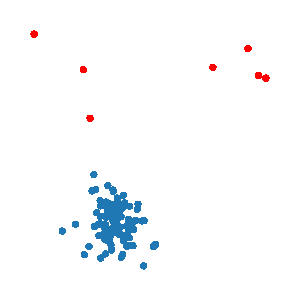
\includegraphics[width=\textwidth]{data/chapter_intro/point_anomalies.pdf}
         \caption{point anomalies}
         \label{fig:point_anomaly}
     \end{subfigure}
     \hfill
     \begin{subfigure}[b]{0.55\textwidth}
         \centering
         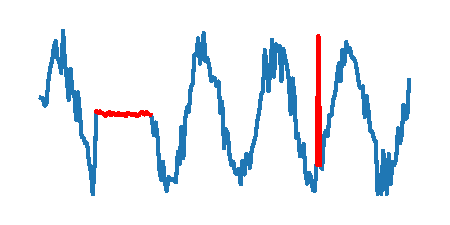
\includegraphics[width=\textwidth]{data/chapter_intro/group_anomalies.pdf}
         \caption{group (left) and contextual (right) anomaly}
         \label{fig:group_anomaly}
     \end{subfigure}

     \vspace{0.1in}

     \begin{subfigure}[b]{0.8\textwidth}
         \centering
         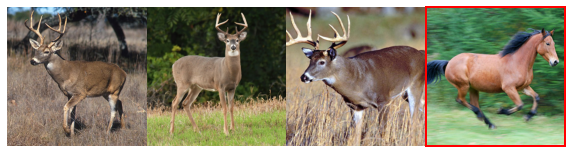
\includegraphics[width=\textwidth]{data/chapter_intro/semantic_anomalies.png}
         \caption{semantic anomaly}
         \label{fig:semantic_anomaly}
     \end{subfigure}

\caption{Examples of different types of anomalies.}
\label{fig:anomaly_examples}
\end{figure}

Different types of anomalies which require different approaches have been identified in literature~\cite{chandola2009anomaly,ruff2020unifying}. Examples are presented in Fig.~\ref{fig:anomaly_examples}.
\begin{itemize}
	\item \textbf{Point anomaly} is a single datapoint of $\mathcal{A}$, for example, an outlying measurement or a photograph of a cat among other images of dogs. This is the most often studied type of anomaly in the research literature. Note that a point anomaly can become an anomaly of the two following types if the datapoints in a dataset are somehow dependent (e.g. through time) or if some additional context about the data can be extracted.

	\item \textbf{Group anomalies} are a collection of correlated datapoints that are only anomalous together. Only a large number of malicious requests is enough to shut down a server in a DDoS atack~\cite{ahmed2018collective}. Other research~\cite{quellec2016multiple,wan2020weakly} focuses on finding anomalies under the multiple-instance learning (MIL)~\cite{carbonneau2018multiple} paradigm, where individual datapoints (called bags) are comprised of a variable number of observations or measurements (called instances). This calls for an aggregation method, on top of which an anomaly detector can operate.

	\item \textbf{Contextual} anomaly is a kind of anomaly that is only anomalous in a certain context. A person measuring over 195~cm is an outlier in almost any place except a locker room of a basketball team. If a target dataset consists of pictures of birds photographed mid-flight -- is a bird sitting on grass an anomaly? Or a different flying object, such as an airplane? The answers to those questions depend on what problem is actually being solved. Contextual anomalies often arise in time series~\cite{tsay2000outliers} or in spatial data~\cite{chawla2006slom}.

	\item \textbf{Semantic} anomalies arise in image data and are opposed to \textbf{sensory} anomalies. While sensory anomalies appear in low-level image features such as edges or textures (e.g. breaks or defects), semantic anomalies can be detected in the high-level information of an image (e.g. an object of a different category than what appears in the  training dataset). Semantic anomalies can be hard to detect, as they can be very similar to normal data~\cite{ahmed2020detecting}. We will cover their detection in chapters~\ref{sec:chapter_comparison} and~\ref{sec:chapter_sgvaegan}.
\end{itemize}

We define the \textbf{contamination rate} of a dataset $X = \lbrace \vc{x}_1, \vc{x}_2, \ldots, \vc{x}_n \rbrace \subset \mathcal{X}$, which is a finite collection of samples from data space $\mathcal{X}$ as
\begin{equation} \label{eq:contamination_rate}
C(\mathcal{X})=\frac{|\{\vc{x}_{i}|\vc{x}_{i}\in \mathcal{A} \wedge \vc{x}_i \in X \}_{i=1}^n|}{|X|},
\end{equation}
i.e. the ratio of the number of anomalies to the total size of the dataset. We can think of any anomaly detection model as providing a function that produces a ranking of the individual data points with respect to their anomalousness. This is called an \textbf{anomaly score} $s:\mathcal{X}\rightarrow\mathbb{R}$ of a model. In certain contexts~\cite{pedregosa2011scikit}, anomaly score might be called \textit{decision }or \textit{scoring function}. In this text, we will assume that a higher anomaly score is attributed to a point more likely to be anomalous. To be able to use an anomaly score for decision-making, one must choose the threshold $\tau\in\mathbb{R}$. From~\eqref{eq:anomaly_set}, a sample $\vc{x}$ is considered to be an anomaly if $s(\vc{x})>=\tau$ and normal otherwise. The selection of $\tau$ can sometimes be a process more complicated than the fitting of the actual model~\cite{ali2013automated}.  Its value is typically determined on the basis of the tolerated false positive rate and an estimate of the true contamination rate of a dataset~\eqref{eq:contamination_rate}.


\section{Comparing anomaly detectors}
Comparing different models on the same set of data is a basic requirement in practical and research problems. As already mentioned at the beginning of this chapter, anomaly detection has some common ground with binary classification tasks. Therefore, we can readily apply the evaluation metrics that are used to evaluate these tasks in comparisons of anomaly detectors. However, there are specifics of anomaly detection problems, mainly the often encountered large imbalance of labeled normal and anomalous samples, that we have to keep in mind. Also, with one exception, all the metrics that will be described here require at least some labeled anomalous samples, no matter how difficult it might be to obtain them. A more complete overview can be found in~\cite{sokolova2006beyond}.

\begin{table}
\centering
	\begin{tabular}{c | c c}
		true label/estimated label & normal & anomalous \\
		\hline
		normal & tn & fp  \\
		anomalous & fn & tp 
	\end{tabular}
	\caption{A confusion matrix of a model which captures the perfromance of a model by showing the total number of correctly (tp = true positives and tn = true negative) and incorrectly (fp = false positives and fn = false negatives) identified samples. In context of anomaly detection, positive samples are anomalies, while normal samples are considered negative.}
	\label{tab:conf_ex}
\end{table}
Table~\ref{tab:conf_ex} displays a confusion table that introduces the basic concepts and notation needed below. It summarizes the performance of an algorithm with a particular threshold.

\subsubsection{AUC}
The most widely used measure in the field of anomaly detection is the area under the ROC (receiver operating characteristic) curve. The acronym AUC will be used in this text for the sake of brevity). The ROC curve is a parametric curve describing the trade-off between \textbf{true positive rate} (sometimes also called \textbf{recall}) $\text{TPR}(\tau) = \frac{\text{tp}}{\text{tp+fn}}(\tau)$ and \textbf{false positive rate} $\text{FPR}(\tau) = \frac{\text{fp}}{\text{fp+tn}}(\tau)$ for different values of the decision threshold $\tau$. 

Then, the area under the curve is calculated as the following integral
\begin{equation} \label{eq:auc}
\text{AUC}=\int_{\mathbb{R}}\text{TPR}(\tau)d\text{FPR}^{\prime}(\tau)d\tau = \int_0^1\text{TPR}(\text{FPR})d\text{FPR}.
\end{equation}
The last integral that uses $\text{TPR}(\cdot)$ as a function of the corresponding FPR shows the simple concept behind the AUC that can be easily discerned from an ROC curve drawn in a graph. An AUC value of 1.0 is equal to perfect classification, while a value of 0.5 is equal to classifying by random guessing. An example of an ROC curve and the corresponding AUC is in Figure~\ref{fig:ROC}. In practice, the corresponding AUC is estimated from an empirical ROC curve using some numerical integration scheme, e.g. the trapezoidal rule.

As mentioned above, the main advantage of AUC is that it does not depend on the choice of a particular decision threshold. Also, the measure has a straightforward interpretation -- it is an estimate of the probability that a randomly chosen positive sample is ranked higher than a randomly chosen negative sample \cite{hand2001simple}. However, a lot of information is lost when the whole ROC curve is summarized into a single number. This is especially concerning for the case of anomaly detection, where usually the region of low false positive rates is of interest since anomalies are sparse with respect to normal data and we strive to achieve a low false positive rate. It is frequent in security applications to draw an ROC curve in logarithmic scale on the x-axis.

\begin{figure}
\centering
\begin{subfigure}[b]{0.45\textwidth} 
	\centering
	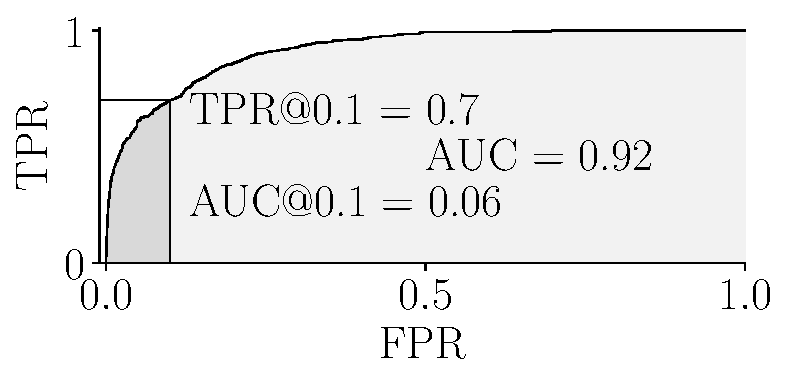
\includegraphics[width=\textwidth]{data/chapter_intro/roc_example.pdf}
	\caption{ROC curve}
	\label{fig:roc_example}
\end{subfigure}
\hfill
\begin{subfigure}[b]{0.45\textwidth}
	\centering
	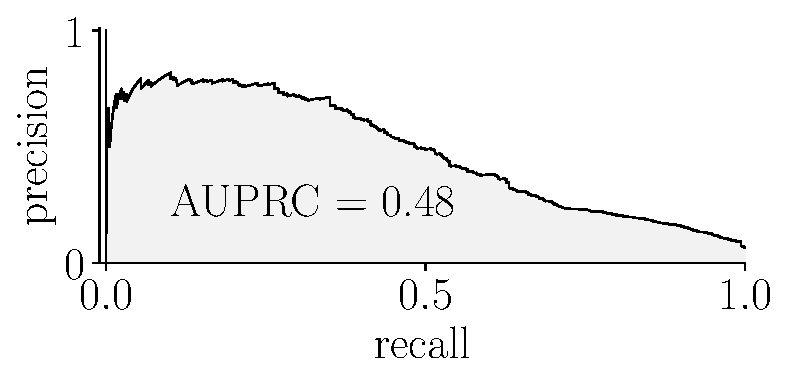
\includegraphics[width=\textwidth]{data/chapter_intro/prc_example.pdf}
	\caption{PR curve}
	 \label{fig:prc_example}
\end{subfigure}
\caption{An example of an ROC curve and the derived measures based on FPR=0.1. AUC is the whole shaded area under the ROC curve. The darker shading corresponds to AUC@0.1. On the left, the PR curve of the same detector is shown.}
\label{fig:ROC}
\end{figure}

\subsubsection{AUPRC}
The Area Under the Precision--Recall Curve is very similar to AUC, as it is given by computing the \textbf{precision} $\text{PREC}(\tau)=\frac{\text{tp}}{\text{tp + fp}}(\tau)$ and recall for different values of classification threshold $\tau$ and then integrating the area under the resulting curve. A PR curve has at most as many unique recall values as positive samples in the dataset. This is problematic for anomaly detection, where the number of anomalies is low, which leads to a very sparse estimate of the true PR curve. In fact, using the same trained anomaly detector and changing the contamination rate of a testing dataset produces different AUPRC results, which then makes any analysis based on AUPRC useless when the true contamination rate is unknown. Furthermore, a correct PR curve lacks a universal starting point, unlike an ROC curve, because precision is undefined for zero recall, making the computation and normalization of the area under the PR curve and the comparison between datasets even more complicated. It is still a metric that is reported very often besides the AUC.

\subsubsection{Areas of low TPR}
The two already mentioned metrics put the same weight on all areas on the x-axis. This might not be always ideal for the purposes of anomaly detection, as low FPR areas might be more interesting -- after all, when reporting detected anomalies for a manual check, there is always a limit on how many samples can be realistically processed. A performance measure popular among practitioners is \textbf{\tpra}, which is simply the true positive rate evaluated at a given false positive rate $\alpha \in [0,1]$. This measure can be easily read from an ROC curve. In practice, it is necessary to interpolate the ROC curve since FPR has discrete values, especially for datasets with a small number of samples. 

Another alternative to AUC is \textbf{\auca}, which is the area under the ROC curve calculated only up to some value of false positive rate $\alpha$. Numerically, it is again important to interpolate the ROC curve for a given $\alpha$ before computing the integral. In Fig.~\ref{fig:ROC}, AUC@0.1 corresponds to the darker gray region. \auca\ can be easily normalized by dividing by the chosen $\alpha$, in which case the best detector has $\auca = 1$ similarly to AUC.

\subsubsection{Volume of decision region}
\begin{figure}
\centering
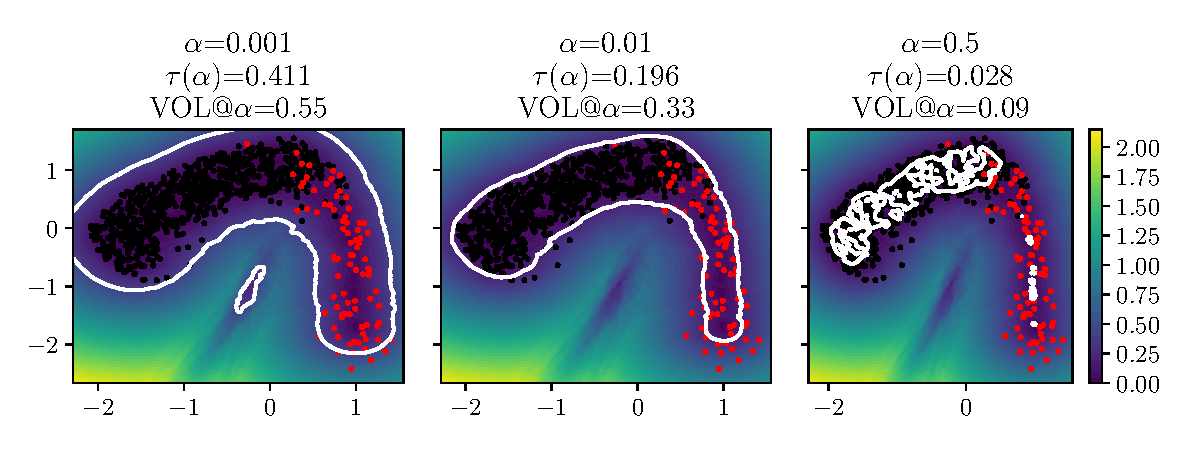
\includegraphics[scale=0.8]{data/chapter_intro/fig_vol_example.pdf}
\caption{An example of a detector and the decision region for differing values of FPR $\alpha$. The decision boundary is drawn as a white isoline at level $\tau(\alpha)$ with the estimated enclosed volume $\text{VOL@}\alpha$, black and red dots represent normal and anomalous samples in the training set. Clearly, smaller tolerance of false positives forces us to set a higher threshold which results in higher decision region volume.}
\label{fig:vol_example}
\end{figure}
All of the previous measures originate from the evaluation of the performance of binary classifiers. Since labeled anomalies are often difficult to obtain, a measure that does not require labels for its evaluation might be more useful and better describe behaviour on unknown samples. If the goal is to compare two models supposed to characterize the normal class, and with no other assumptions about the distribution of the anomalous class, it makes sense to choose the model enclosing the training data more tightly. This corresponds to calculating the volume inside the model's decision boundary in a similar fashion to \cite{clemenccon2013scoring}, where a theoretical justification is given. This decision boundary can be chosen to correspond to a certain level of false positive rate. We define the \textbf{volume of decision region} as
\begin{equation}
  \text{VOL}(\alpha) = \int_{\mathcal{X}} \mathds{1}_{\lbrace \vc{x} \in\mathcal{X}|s(\vc{x}) <= \tau\rbrace} \left( \vc{x} \right) d\vc{x}  \text{ s.t. } \text{FPR}(\tau)=\alpha,
\end{equation}
where $\mathcal{X}$ is the input space, $s(\vc{x})$ is an anomaly score, and $\alpha$ is a given false positive rate. In other words, $\text{VOL}(\alpha)$ is the volume of the subspace where the classifier returns "normal" answer with a false positive rate $\alpha$. An example of a model and its decision region for different values of $\alpha$ is shown in Fig.~\ref{fig:vol_example}. It should be noted that the idea of minizing the enclosed volume is native to some models, e.g. the SVDD model described in Sec.~\ref{sec:domain_methods}.

Computing the empirical $\text{VOL}(\alpha)$ in data space $\mathcal{X}$ requires first finding the threshold $\tau$ corresponding to the chosen FPR $\alpha$ and then integrating the volume which corresponds to the space enclosed by the isosurface where the anomaly score is equal to $\tau$. It is numerically estimated by Monte Carlo sampling~\cite{robert1999monte}. This comes with its downsides. Mainly, the number of samples required to cover $d$--dimensional sample space grows exponentially with $d$. This issue has been addressed in \cite{goix2016evaluate}, where the volume is computed multiple times for different subsampling of input features, however this does not seem to be optimal as it requires training a new model for each subset of features.


\section{Anomaly detectors taxonomy} \label{sec:taxonomy}
Anomaly detection methods are based on a wide range of paradigms. In this section we will follow the taxonomy outlined in publications~\cite{pimentel2014review, ruff2020unifying}, which divide shallow (not based on neural networks) and deep (based on neural networks) detectors into groups based on their common traits. Examples of methods will be given since their knowledge will be useful in the later chapters of this text, but the list is far from complete. For a complete overview of the landscape of anomaly detection methods, see the surveys~\cite{pimentel2014review, campos2016evaluation, goldstein2016comparative, moustafa2019holistic, kwon2019survey, fernandes2019comprehensive, wang2019progress, chalapathy2019deep,ruff2020unifying}.

\subsection{Probabilistic  methods} \label{sec:probabilistic_models}
Since we have defined anomaly detection as detecting samples that deviate from the normal distribution $P^+$, it is straightforward to try to model the distribution by modeling its probability distribution function (pdf). One of the simplest such methods is the Grubbs' test~\cite{grubbs1969procedures}, which assumes a Gaussian distribution of normal one-dimensional data and declares a sample to be anomalous if its distance from the mean is larger than some threshold (e.g. three standard deviations). Many such methods based on statistical tests have been proposed~\cite{barnett1994outliers}, but we will focus on advanced modeling probabilistic techniques.

\subsubsection{Shallow methods}
A \textbf{Mahalabonis distance} anomaly detector~\cite{laurikkala2000informal} builds a parametric estimate of a multivariate normal distribution by computing the mean $\vc{\mu} \in \mathbb{R}^d$ and covariance matrix $\Sigma \in \mathbb{R}^{d,d}$ of the training data. The anomaly score of a test point $\vc{x} \in \mathbb{R}^d$ is then
\begin{equation} \label{eq:mahalabonis_score}
	s(\vc{x}) =  (\vc{x} - \vc{\mu}) ^T \Sigma ^{-1} (\vc{x}-\vc{\mu}),
\end{equation}
which is equivalent to the evaluation of the negative log-likelihood under the Gaussian distribution. Even though this is one of the simplest and most non-robust methods, terms similar to~\eqref{eq:mahalabonis_score} will be encountered a lot in the remainder of this text.

Instead of limiting the model to a single-mode distribution, a mixture of $K$ distributions 
\begin{equation} \label{eq:mixture}
	p(\vc{x}) = \sum_{k=1}^K p(k) p(\vc{x}|k), p(k) \in [0,1], \sum_{k=1}^K p(k) = 1,
\end{equation}
can be estimated instead, where $p(k)$ is the prior probability of the $k$-th component. \textbf{Gaussian Mixture Models} (GMMs) have been used for anomaly detection in~\cite{roberts1994probabilistic,mahadevan2010anomaly}. There, we assume that $p(\vc{x}|k)$ are Gaussian distribution densities and their parameters are estimated using the EM algorithm~\cite{dempster1977maximum} or via Variational Bayes~\cite{bishop2006pattern}. The term $-\log p(\vc{x})$ is usually used as the anomaly score, although sometimes the maximum of the Mahalabonis distance~\eqref{eq:mahalabonis_score} over the $K$ components is used instead. However, the viable usecases for a GMM anomaly detector are limited, mainly due to the need to compute and invert the covariance matrix, which is $O(d^3)$ in the size of the input space $d$ (when the full covariance matrix is estimated). See Fig.~\ref{fig:gmm_examples}, where the same anomaly detection problem is solved by GMMs with different number of components. Even though the AUC score is already perfect for 2 components, the difficult shape of the normal data needs more components than that to be fully covered.

Time series data anomaly detection was approached with the use of \textbf{Autoregressive Integrated Moving Average} (ARIMA) models in~\cite{roberts1994probabilistic,hoare2002line}, or using a \textbf{Hidden Markov Model} (HMM) in~\cite{yeung2003host,zhang2003new}. Both approaches offer predictions for future states of an observed system, and the anomaly score is the difference between the prediction and the actual state of the system. The problems to which these methods can be applied are encountered in medicine or computer network intrusion detection.

All the previous were examples of parametric models, where a set of parameters $\vc{\theta}$ is directly estimated. Opposed to these are non-parametric models, which are less restricting  -- e.g. they do not assume any (normal, Poisson, ...) distribution -- instead, they build a parameter-free model of the normal data. \textbf{Kernel density estimation} (KDE) method~\cite{parzen1962estimation}, which estimates an unknown univariate probability density function by an empirical estimate
\begin{equation} \label{eq:kde}
	\hat{p}(x) = \frac{1}{hn} \sum_{i=1}^n k_f \left( \frac{x-x_i}{h} \right), x_i \in X
\end{equation}
where $X = \lbrace x_1, x_2, \ldots, x_n \rbrace$ is the training dataset of $n$ samples, $h \in \mathbb{R}^+$ is a bandwidth parameter, and $k_f:\mathbb{R} \rightarrow \mathbb{R}^+$ is a kernel function (uniform, triangular, normal, etc.). KDE has been used under the name Parzen window estimate e.g. in~\cite{tarassenko1995novelty,yeung2002parzen}, where $-\ln \hat{p}(x)$ is used to score anomalies. \textbf{Histogram-based Outlier Score} (HBOS) is a method~\cite{goldstein2012histogram} for anomaly detection on multivariate data $\vc{x} \in \mathbb{R}^d$. It computes normalized histograms for each feature $x_j$ independently. Then the anomaly score for an unlabeled sample $\vc{x}$ is
\begin{equation} \label{eq:hbos}
	s(\vc{x}) =  -\sum_{j=1}^d \ln \tilde{p}_j(\vc{x})
\end{equation}
where $\tilde{p}_j(\vc{x})$ is the height of the bin in which $x_j$ is located. The main advantage of this method in comparison with e.g. distance-based is the relative computational simplicity. In the \textbf{Lightweight Online Detector of Anomalies} (LODA)~\cite{pevny2016loda}, an ensemble of one-dimensional histograms is used in a space of diversified projection vectors. The anomaly score is then an average of the logarithm of probabilities estimated from the histograms on individual projection vectors. Due to its simplicity and computational efficiency, it is popular in settings with high volumes of data and potentially missing input values.

\begin{figure}
\begin{centering}
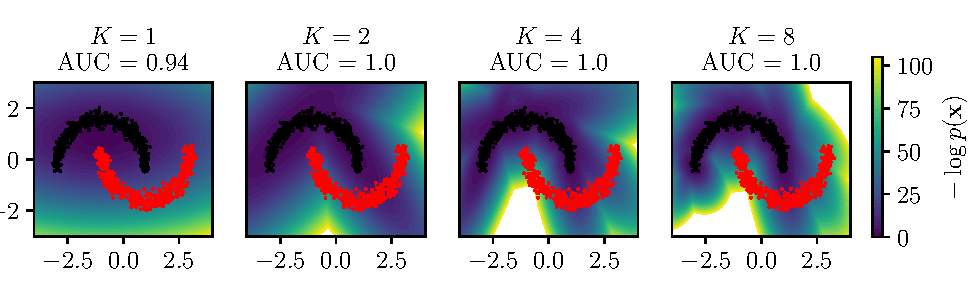
\includegraphics[scale=0.98]{data/chapter_intro/gmm_examples.pdf}
\end{centering}
\caption{The \textit{two bananas} dataset consists of two clusters of points. The black points are considered to be normal and the red are considered to be anomalies. The dataset is useful for introducing behaviour of anomaly detectors, because as an anomaly detection problem, it cannot be solved by a linear separation of the two groups of points. Here, GMM models with a varying number of components $K$ are fitted to the normal datapoints. The contours of the anomaly score based on~\eqref{eq:mixture} are shown together with the AUC computed with respect to the anomalous datapoints.}
\label{fig:gmm_examples}
\end{figure}

\subsubsection{Deep methods}
The recent advent of neural networks has given rise to many novel methods that are more capable of handling high-dimensional datasets that would be otherwise extremely difficult to handle. A mixture model was used in the \textbf{DAGMM} method~\cite{zong2018deep}, where a neural network creates a low-dimensional latent representation $\vc{z}$ from an input $\vc{x}$. The GMM and its parameters are then estimated in the latent space, again via a neural network, which enables online learning of the whole model together.

\textbf{Energy based models} (EBMs) use the energy function $E_{\vc{\theta}}(\vc{x})$ to approximate the density as
\begin{equation} \label{eq:ebm}
	p_{\vc{\theta}}(\vc{x}) =  \frac{1}{Z(\vc{\theta})} \exp (- E_{\vc{\theta}}(\vc{x})),
\end{equation}
where $Z(\vc{\theta})$ is the partition function parametrized by $\vc{\theta}$ to ensure proper normalization of $p_{\vc{\theta}}(\vc{x})$. Although the partition function usually cannot be directly computed, an EBM can still be trained via gradient descent coupled with Markov Chain Monte Carlo estimation~\cite{hinton2002training}, which is however also the reason for its ineffectiveness relative to more novel approaches, as the MCMC is computationally costly. The anomaly score is then the energy function $E_{\vc{\theta}}(\vc{x})$. Although the direct use of the early examples of EBMs such as \textbf{Deep Belief Networks}~\cite{hinton2006fast} and \textbf{Deep Boltzmann Machines}~\cite{salakhutdinov2010efficient} was impractical for anomaly detection, they were eventually refined and successfully used on anomaly detection benchmarks in~\cite{zhai2016deep}. 

Finally, the most recent advancements in anomaly detection were achieved with the use of deep generative models that model the distribution of the data via a generative process, where it is assumed that the data is generated from a hidden latent variable. \textbf{Flow models}~\cite{dinh2014nice}, \textbf{Variational autoencoders}~\cite{kingma2013vae} and \textbf{Generative Adversarial Networks}~\cite{goodfellow2014gan}  will be described in greater detail in Chapter~\ref{sec:chapter_survey}.

\subsection{Distance-based methods} \label{sec:distance_methods}
Instead of modeling the probability distribution of the normal data, distance-based anomaly detectors use heuristics that compute a well-defined similarity measure between two data points. One of the simplest such models is the \textbf{k-Nearest Neighbor} (kNN)~\cite{ramaswamy2000efficient} model where the anomaly score of a sample is based on its proximity to its $k$--nearest neighbours from the training dataset. Different proximity measures are described in~\cite{harmeling2006outliers}, where 
the Euclidean distance is used as the similarity measure and the set $X_{k}(\vc{x})$ is defined as the set of $k$-nearest neighbors of $\vc{x}$ from a training dataset $X = \lbrace \vc{x}_1, \vc{x}_2, \ldots, \vc{x}_n \rbrace \subset \mathbb{R}^d$.
\begin{itemize}
	\item $\kappa(\vc{x})$: the anomaly score is the distance between $\vc{x}$ and its $k$th-nearest neighbor,
	\begin{equation} \label{eq:knn_kappa}
		s_{\kappa}(\vc{x}) =  \max_{\vc{x}_i \in X_k(\vc{x})} \vert \vert \vc{x} - \vc{x}_i \vert \vert_2,
	\end{equation}
	\item $\gamma(\vc{x})$: the anomaly score is the average distance of $\vc{x}$ to its $k$-nearest neighbors, 
	\begin{equation} \label{eq:knn_gamma}
		s_{\gamma}(\vc{x}) =  \frac{1}{k} \sum_{\vc{x}_i \in X_k(x)} \vert \vert \vc{x} - \vc{x}_i \vert \vert_2,
	\end{equation}
	\item $\delta(\vc{x})$: the anomaly score is the length of the mean of the vectors pointing from $\vc{x}$ to its $k$-nearest neighbours,
	\begin{equation} \label{eq:knn_delta}
		s_{\delta}(\vc{x}) =  \left| \left| \frac{1}{k} \sum_{\vc{x}_i \in X_k(x)} (\vc{x}_i - \vc{x}) \right| \right|_2.
	\end{equation}
\end{itemize}
All these definitions presume that normal data lie in concentrated regions of the data space $\mathcal{X}$, according to~\eqref{eq:normal_concentration}, while anomalies lie outside of them. The kNN anomaly detector is very popular thanks to its simplicity and good performance~\cite{campos2016evaluation}. See Fig.~\ref{fig:knn_examples}, where low values of $k$ result in a very local behaviour of the model, which is suitable for this problem. The biggest disadvantage of the model is the computational cost. Even though there is no actual training procedure, the prediction complexity is $O(ndk)$. This can be ameliorated by the construction of a $k$-d tree~\cite{bentley1975multidimensional}, which partitions the space of the training data to speed-up prediction, or using GPU-based similarity search techniques such as~\cite{johnson2019billion}. Other methods, such as \textbf{REPEN}~\cite{pangLearningRepresentationsUltrahighdimensional2018}, use the kNN detector trained on low-dimensional representations of otherwise high-dimensional data produced by a deep neural network.

The \textbf{Local Outlier Factor} (LOF) algorithm~\cite{breunig2000lof} is based on comparing the local density of a sample $\vc{x}$ with the local density of its $k$--nearest neighbours. To correctly describe the way in which the density is defined and the anomaly score is computed, we use the formula~\eqref{eq:knn_kappa}. Then we define the \textit{local reachability density} as 
\begin{equation}
  \text{LRD}_k(\vc{x})=\frac{|X_k(\vc{x})|}{\sum_{\vc{x}_i\in X_k(x)} \max \lbrace s_{\kappa}(\vc{x}), \vert \vert \vc{x} - \vc{x}_i \vert \vert_2 \rbrace }.
\end{equation}
Since this is basically the inverse of an average distance between $\vc{x}$ and its neighbours, the closer the neighbours are to $\vc{x}$, the higher this approximation of local density is. Finally, anomaly score of $\vc{x}$ is given by comparing the $\text{LRD}_k$ of $\vc{x}$ and its neighbours 
\begin{equation}
  s_{\text{LOF}}(\vc{x})=\frac{\sum_{\vc{x}_i\in X_k(\vc{x})} \text{LRD}_k(\vc{x}_i)}{\text{LRD}_k(\vc{x}) |X_k(\vc{x})|}.
\end{equation}
The rationale behind the formula is that if the local density of the neighbours is higher or the local density of $\vc{x}$ is lower then it is more likely for $\vc{x}$ to be an anomaly. This method however does not scale well in number of training samples, as its complexity is even greater than that of a simple kNN detector. Similar methods to LOF are the \textbf{connectivity--based outlier factor} (COF)\,\cite{tang2002enhancing} or \textbf{clustering--based local outlier factor} (CBLOF)\,\cite{he2003discovering}.

\begin{figure}
\begin{centering}
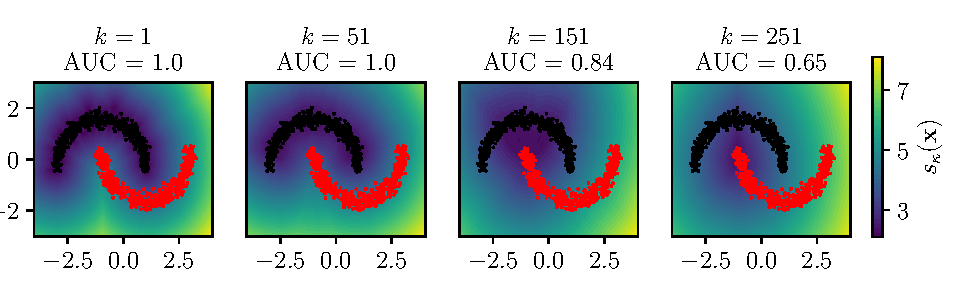
\includegraphics[scale=0.98]{data/chapter_intro/knn_examples.pdf}
\end{centering}
\caption{K-nearest neighbor detectors on the \textit{two bananas dataset}. The contours of the score~\eqref{eq:knn_kappa} are shown for different values of $k$ together with the resulting AUC.}
\label{fig:knn_examples}
\end{figure}

A different approach is taken by the \textbf{isolation forest }(IF) model~\cite{liu2008isolation} where an ensemble of $N_t$ isolation trees is constructed for the whole dataset. Isolation trees are constructed in such a way as to isolate each individual datapoint from the rest of the dataset using consecutive splits on different features. It is presumed that an anomaly can be isolated using a smaller number of splits and therefore it lies on a branch closer to the root of the tree. The anomaly score is then based on the number of splits of a sample averaged over multiple randomly initialized trees in the ensemble. A method similar to IF is the \textbf{Partial Identification Forest} (PIDForest)~\cite{gopalanPIDForestAnomalyDetection2019}, which uses a more informed way of choosing the data features for split, favouring the more informative features.

In \textbf{Angle-Based Outlier Detection} (ABOD)~\cite{kriegel2008angle} presumes that outliers lie far from clusters of normal data, therefore the viewing angle that covers a cluster of normal datapoints when "looking" at it from a sample $x$ is smaller when $x$ is anomalous. More concretely, the method computes the angles between $x$ and all pairs of points in the training dataset, and the anomaly score is inversely proportional to the variance of these angles -- the more varied the angles are, the more likely $x$ is close to some cluster of normal data and the anomaly score is thus lower. In the original paper, the method is lauded for the lack of hyperparameters that need to be tuned and the ability to operate in high-dimensional data spaces. However, in the experiments in Chapter~\ref{sec:chapter_comparison}, it proves to be the method with one of the slowest prediction times.

\subsection{Domain-based  methods} \label{sec:domain_methods}
\subsubsection{Shallow methods}
In domain-based models, the data space is partitioned into subspaces by a decision boundary. Instead of estimating the density of the whole training dataset, they only consider a few samples from it, which are called \textit{support vectors}, and which are used to define the decision boundary. A very simple example is an anomaly detector which, for a training set $X = \lbrace \vc{x}_1, \vc{x}_2, \ldots, \vc{x}_n \rbrace \subset \mathbb{R}^d$, constructs a hypersphere with center $\vc{c} \in \mathbb{R}^d$ and radius $R>0$ that encloses the training data. It is found by solving the objective
\begin{alignat}{1}
\mathclap{
	\begin{aligned}
	\min_{R,\vc{c},\vc{\xi}} R^2 & + \frac{1}{\nu n}\sum_{i=1}^n \xi_i \\
	\text{s.t.} \vert \vert \vc{x}_i - \vc{c} \vert \vert_2^2 & \leq R^2 + \xi_i, \xi_i \geq 0, \forall i
\end{aligned}
} \label{eq:hypersphere}
\end{alignat}
where $\xi_i$ are slack variables that allow some data points to lie outside of the hypersphere. The ratio of the maximum number of outliers is controlled by the variable $\nu \in (0,1]$, which is at the same time a lower bound on the number of support vectors, which are samples $\vc{x}_i$ that lie exactly on the boundary of the hypersphere. The solution to~\eqref{eq:hypersphere} is given by solving the dual problem. Notice that a simple criterion $\vert \vert \vc{x} - \vc{c} \vert \vert_2^2  \leq R^2$ already gives a decision whether the point $\vc{x}$ is already inside the sphere. To convert this to a continuous anomaly score, we can compute the distance of $\vc{x}$ from the boundary
\begin{equation} \label{eq:hypersphere_score}
	s(\vc{x}) = \vert \vert \vc{x} - \vc{c} \vert \vert_2^2 - R^2
\end{equation}
which is negative for points inside and positive for points outside the hypersphere.

Abstracting the above, one can use \textit{kernel functions}~\cite{shawe2004kernel} to move the problem~\eqref{eq:hypersphere} from the original input space to a transformed kernel space. The kernel is a function $k_f:\mathbb{R}^d \times \mathbb{R}^d \rightarrow \mathbb{R}$, with which we associate a \textit{feature map} $\Phi: \mathbb{R}^d \rightarrow \mathcal{F}_k$ such that the relation defined by the inner product $k_f(\vc{x},\vc{y})=\langle \Phi(\vc{x}), \Phi(\vc{y}) \rangle$ is true for all $\vc{x},\vc{y}$. The space $\mathcal{F}_k$ is a reproducing kernel Hilbert space and we choose the kernel in such a way that its dimensionality is higher than $d$. This is the basis for the \textbf{Support Vector Data Descriptor} (SVDD) anomaly detector, where the inequality condition in~\eqref{eq:hypersphere_score} is replaced by $\vert \vert \Phi(\vc{x}_i) - \vc{c} \vert \vert_2^2 \leq R^2 + \xi_i$. By solving the problem in a space of higher dimensionality, it is possible to find a decision boundary (hypersphere) for datapoints that would otherwise not be separable in the original space. In comparison, the \textbf{One-Class Support Vector Machine} (OCSVM)~\cite{scholkopf2001estimating} does not construct a hypersphere, but instead aims to find a separating hyperplane in the kernel space. See Fig.~\ref{fig:ocsvm_examples} for a demonstration of the OCSVM model on our toy dataset.  Unlike in traditional SVM~\cite{cortes1995support}, which is used to separate two classes in a binary classification problem, OCSVM instead aims to find a hyperplane that maximizes the separation of the majority of the training data from the origin in the kernel space. The anomaly score of an OCSVM detector is, similarly to~\eqref{eq:hypersphere_score}, the distance from the separating hyperplane. Apart from $\nu$, a very important hyperparameter of the model is the kernel scale parameter $\gamma_{\text{OCSVM}}$. Many variants of both of the presented approaches were introduced over the years, such as \textbf{Minimum Volume Ellipsoid}~\cite{van2009minimum}, \textbf{Multi-sphere SVDD}~\cite{gornitz2017support} or \textbf{Bayesian Data Description}~\cite{ghasemi2012bayesian}.

\begin{figure}
\begin{centering}
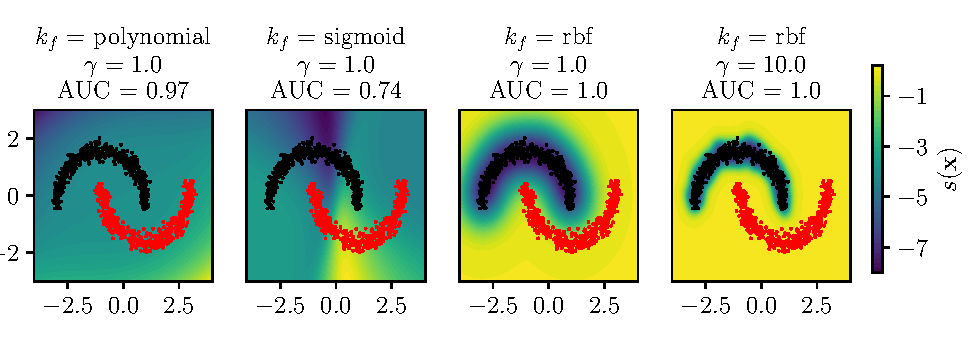
\includegraphics[scale=0.98]{data/chapter_intro/ocsvm_examples.pdf}
\end{centering}
\caption{OCSVM detectors with different kernel functions and kernel width parameter $\gamma$ values on the \textit{two bananas dataset}. The contours of the score~\eqref{eq:hypersphere_score} together with the resulting AUC. Although the use of both the polynomial and sigmoid kernels results in a relatively good AUC value, the anomaly score contours reveal that the model would fail if the anomalies would be placed slightly differently. On the other hand, the tight fit of the training data with the \textit{radial basis function} (rbf) is proportional to the kernel width.}
\label{fig:ocsvm_examples}
\end{figure}

\subsubsection{Deep methods}
Instead of choosing a kernel and its parameters manually, one can instead parametrize the feature maps $\Phi$ using neural networks and train them using standard gradient descent techniques, or use pretrained networks from related tasks. This is the basis for deep OCSVM methods such as \textbf{One-class Neural Network} (OCNN)~\cite{chalapathy2018anomaly} or~\cite{erfani2016high}, or methods based on the SVDD formulation~\cite{ghafoori2020deep}. In \textbf{Deep SVDD} (DSVDD)~\cite{ruff2018deep}, the objective~\eqref{eq:hypersphere} is reformulated without the slack variables $\xi_i$, which means that the hypersphere is expected to enclose all datapoints in the training dataset. This simplification leads to faster convergence and yet still proves to be an effective anomaly detector. However, all the deep methods have a basic flaw. Without any further restrictions, the solution $\Phi(\vc{x}) = \vc{c}$ is valid but does not provide a useful detector. This behaviour is called the \textit{feature map collapse}. In order to prevent this, many techniques such as freezing the neural networks that provide the feature map, architectural choices or using adversarial learning are used (for an extensive list of possibilities, see~\cite{ruff2020unifying}).

\subsubsection{Training with negative examples}
Although we have stated in Sec.~\ref{sec:ad_definition} that anomaly detection methods do not usually consider the distribution of anomalies $P^-$, there are some approaches that do. These still fall under the domain-based category of anomaly detectors, as they are mostly constructed as binary classifiers that divide the input space into subspaces where either the anomalous or normal class is expected. In the simplest case~\cite{steinwart2005classification}, $P^-$ is assumed to be uniform and a supervised classifier is trained using anomalies sampled from a hypercube centered around the normal data. This approach however suffers from the curse of dimensionality and saturating the hypercube in high-dimensional spaces is computationally infeasible, especially for image data. Some attempts for a more efficient sampling have been proposed, such as sampling based on local density esimation~\cite{fan2004using}. In \textbf{outlier exposure}~\cite{hendrycksDeepAnomalyDetection2019} techniques, a large auxiliary dataset, that is somehow related to normal data, is used to improve the generalization properties of a deep anomaly detector. For example, if the normal class consists of images of birds, it might be useful to train the detector to recognize normal data from images containing other animals, even though this auxiliary dataset may contain animal classes that will not be encountered as anomalies in test/production environment. It has been shown to be an effective technique in~\cite{hendrycks2019using}.  

Outlier exposure is a form of \textbf{weak supervision}~\cite{zhou2018brief}, which is a more general term covering the approach to learning with imperfectly labeled anomaly samples. In~\cite{ruff2019deep,liznerski2020explainable} it is shown that using even a few labeled examples of anomalies can dramatically improve the detection performance. It is however important to robustify the model in order to be able to generalize to the types of anomalies not present in the labeled training dataset. These techniques can help in \textbf{active learning} in anomaly detection~\cite{abe2006outlier}, where the anomaly detector sends queries to its operator, asking for the most informative/relevant samples to be manually labeled. It is stated in~\cite{ruff2020unifying} that weak supervision is essential for potential breakthroughs in anomaly detection, which is the motivation for the method proposed in Chapter~\ref{sec:chapter_sgvaegan}.

Another paradigm where the model is trained in the presence of additional data is \textbf{self-supervision}~\cite{kolesnikov2019revisiting}, where the model solves an auxiliary task, such as prediction of transformations applied to the image~\cite{chen2020simple}. The important distinction between this approach and outlier exposure is that the transformed data is obtained from the normal training dataset by applying random translations, scalings, rotations, etc. Transforming the data in a controlled manner, the anomaly detector is then a multiclass classifier that predicts the correct transformation applied to the data. The anomaly score of such a model is then based on the softmax activations in the output layer -- if the prediction uncertainty is high, the scored sample is more likely to be an anomaly. This was very successfully used in the \textbf{Geometric Transformations} (GT)~\cite{golan2018deep} anomaly detector. Furthermore, the \textbf{GOAD} method~\cite{bergman2020classification} extends this approach to non-image data.

\subsection{Reconstruction-based methods} \label{sec:reconstruction_models}
One of the most popular approaches to anomaly detection is to build a model that learns to reconstruct input samples. When this model is trained on normal data and learns to reconstruct them well, it is expected that it will be able to identify anomalies by failing to reconstruct them properly, since they have properties unseen by the model at training time. To formalize this, a reconstruction-based anomaly detector consists of an \textit{encoder}, which is a mapping $e_{\vc{\phi}}:\mathcal{X} \rightarrow \mathcal{Z}$, and a \textit{decoder} $g_{\vc{\theta}}: \mathcal{Z} \rightarrow \mathcal{X}$. Here, $\mathcal{X} \subset \mathbb{R}^d$ is the input space, $\mathcal{Z} \subset \mathbb{R}^h$ is a so called \textit{latent} space and $\vc{\phi},\vc{\theta}$ are parameters. A \textit{latent representation} or \textit{encoding} of a sample $\vc{x}$ is $z = e_{\vc{\phi}}(\vc{x})$. Reconstruction-based methods then try to match the original sample $\vc{x}$ with its reconstruction $\vc{x}' = g_{\vc{\theta}}(\vc{z})=g_{\vc{\theta}}(e_{\vc{\phi}}(\vc{x}))$. This is done by finding such parameters $\vc{\phi}, \vc{\theta}$ as to minimize the reconstruction objective
\begin{equation} \label{eq:reconstruction_objective}
	\min_{\vc{\phi}, \vc{\theta}} \vert \vert \vc{x} - g_{\vc{\theta}}(e_{\vc{\phi}}(\vc{x})) \vert \vert_2^2 + \mathcal{R},
\end{equation}
where $\mathcal{R}$ is a regularization term. Some sort of regularization is needed in order to prevent the decoding function $(g_{\vc{\theta}} \circ e_{\vc{\phi}})(\vc{x})$ to become an identity function, in which case the detector would be useless. The anomaly score of reconstruction-based methods is the \textit{reconstruction error}
\begin{equation} \label{eq:reconstruction_error}
	s(\vc{x}) = \vert \vert x - g_{\vc{\theta}}(e_{\vc{\phi}}(\vc{x})) \vert \vert_2^2.
\end{equation}


The \textbf{Principal Component Analysis} (PCA)~\cite{shyu2003novel,aggarwal2015outlier}, although not originally developed for this purpose, is an example of a reconstruction anomaly detection method. It is assumed that the normal data lie on a lower-dimensional manifold in the data space, which is an assumption also used in other methods. This means that theoretically, they can be represented by a transformation into a lower dimensional latent space, and the eventual differences between the reconstructions from the latent back to the data space and the original samples are only due to noise that is present in the data, and therefore the latent representation contains all the relevant information of a sample. PCA seeks to represent the data by finding an orthonormal basis $W \in \mathbb{R}^{h,d}$ that maximizes the empirical variance of the data $X= \lbrace \vc{x}_1, \vc{x}_2, \ldots, \vc{x}_n \rbrace \subset \mathbb{R}^d$. The original objective of PCA can be reformulated with~\eqref{eq:reconstruction_objective} in mind, which yields 
\begin{equation} \label{eq:pca}
	\max_W \sum_{i=1}^n \vert \vert \vc{x}_i -  W^TW \vc{x}_i \vert \vert_2^2, \text{s.t.} WW^T = I.
\end{equation}
Thus, this means $\vc{z} = e_{\vc{\phi}}(\vc{x}) = W \vc{x} \in \mathbb{R}^h$ is the encoding represented by the first $h$ \textit{principal components}, while the decoder is $g_{\vc{\theta}}(\vc{z}) = W^T\vc{z}$. The solution to~\eqref{eq:pca} is obtained by collecting the first $h$ eigenvectors of the covariance matrix of the training data, e.g. through its eigendecomposition, or by computing the \textit{singular value decomposition} of the data matrix. Like in the domain-based methods in Sec.~\ref{sec:domain_methods}, some of the restrictions imposed by the linear formulation of classical PCA are circumvented by using a \textbf{kernel PCA} (kPCA)~\cite{scholkopf1998nonlinear}, where $x$ is replaced by its nonlinear transformation $\Phi(\vc{x})$. This was used for anomaly detection e.g. in~\cite{xiao2013l1}.

\begin{figure}
\begin{centering}
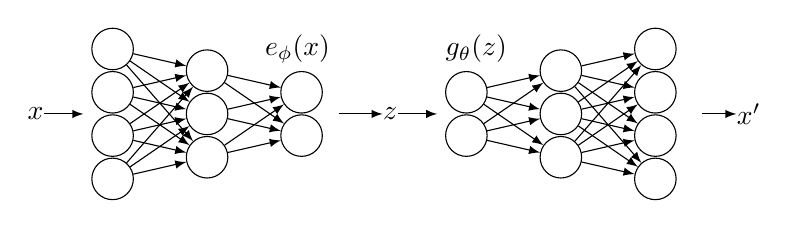
\begin{tikzpicture}
  \node[const]                               (x) {$\vc{x}$};
  \node[const, right = 0.5cm of x]           (xin) {};
  % encoder in
  \node[latent, right = 0.6cm of x, yshift = 0.825cm] (E11) {};
  \node[latent, right = 0.6cm of x, yshift = 0.275cm] (E12) {};
  \node[latent, right = 0.6cm of x, yshift = -0.275cm] (E13) {};
  \node[latent, right = 0.6cm of x, yshift = -0.825cm] (E14) {};
  % encoder hidden
  \node[latent, right = 1.8cm of x, yshift = 0.55cm] (E21) {};
  \node[latent, right = 1.8cm of x, yshift = 0cm] (E22) {};
  \node[latent, right = 1.8cm of x, yshift = -0.55cm] (E23) {};
  % encoder out
  \node[latent, right = 3cm of x, yshift = 0.275cm] (E31) {};
  \node[latent, right = 3cm of x, yshift = -0.275cm] (E32) {};
  % encoder tag
  \node[const, right = 2.8cm of x, yshift = 0.825cm] (E) {$e_{\vc{\phi}}(\vc{x})$};
  % code
  \node[const, right = 4.3cm of x]           (z) {$\vc{z}$};
  \node[const, right = -0.8cm of z]           (zout) {};       
  \node[const, right = 0.5cm of z]           (zin) {};
  % decoder in
  \node[latent, right = 0.6cm of z, yshift = 0.275cm] (D11) {};
  \node[latent, right = 0.6cm of z, yshift = -0.275cm] (D12) {};
  % decoder hidden
  \node[latent, right = 1.8cm of z, yshift = 0.55cm] (D21) {};
  \node[latent, right = 1.8cm of z, yshift = 0cm] (D22) {};
  \node[latent, right = 1.8cm of z, yshift = -0.55cm] (D23) {};
  % decoder out
  \node[latent, right = 3cm of z, yshift = 0.825cm] (D31) {};
  \node[latent, right = 3cm of z, yshift = 0.275cm] (D32) {};
  \node[latent, right = 3cm of z, yshift = -0.275cm] (D33) {};
  \node[latent, right = 3cm of z, yshift = -0.825cm] (D34) {};
  % xhat
  \node[const, right = 4.3cm of z]           (xhat) {$\vc{x}'$};
  \node[const, right = -0.8cm of xhat]       (xhatout) {};       
  % decoder tag
  \node[const, right = 0.6cm of z, yshift = 0.825cm] (D) {$g_{\vc{\theta}}(\vc{z})$};
  

  % edges
  \nedge {x} {xin}
  % encoder 
  \nedge {E11, E12, E13, E14} {E21, E22, E23}
  \nedge {E21, E22, E23} {E31, E32}
  % latent
  \nedge {zout} {z}
  \nedge {z} {zin}
  % decoder
  \nedge {D11, D12} {D21, D22, D23}
  \nedge {D21, D22, D23} {D31, D32, D33, D34} 
  %xhat
  \nedge {xhatout} {xhat}

  % encoder plate
%  \plate {E} {(E11)(E14)(E32)} {};
\end{tikzpicture}

\par\end{centering}
\centering{}\caption{An example of an autoencoder consisting of fully connected layers. The latent code $\vc{z}\in\mathbb{R}^{2}$ is computed by propagating the input $\vc{x} \in\mathbb{R}^{4}$ through the encoder $e_{\vc{\phi}}(\vc{x})$ and then used to produce the reconstruction $\vc{x}'\in\mathbb{R}^{4}$ via the decoder $g_{\vc{\theta}}(\vc{z})$.}
\label{fig:ae}
\end{figure}

\begin{figure}
\begin{centering}
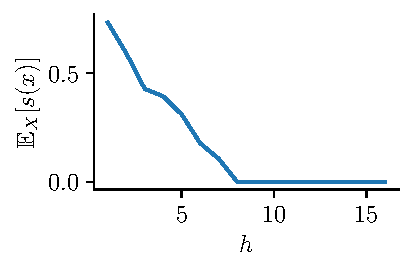
\includegraphics[scale=1.0]{data/chapter_intro/ae_reconstruction}\caption{The figure demonstrates the ability of an autoencoder to reconstruct data. The dimension $h$ of the latent space $\mathcal{Z}$ is on the x--axis, while the average reconstruction error~\eqref{eq:reconstruction_error} over the whole dataset is on the y--axis. Note that although the artificial dataset is 16--dimensional, it only contains 8 non--correlated dimensions while the remaining are a linear combination of them, which makes the data lie on an 8-dimensional manifold. This results in the error dropping to zero for $h>=8$ where the model is able to disentangle the correlations and learn the identity function.}
\label{fig:ae_reconstruction}
\par\end{centering}
\end{figure}

An \textbf{autoencoder} (AE)~\cite{kramer1991nonlinear} is in its basic principle a nonlinear PCA, where the encoder $e_{\vc{\phi}}$ and decoder $g_{\vc{\theta}}$ are neural networks and the parameters $\vc{\phi},\vc{\theta}$ are the trainable weights of these networks. The nonlinearity comes from the use of nonlinear activation functions between the individual layers of the neural networks. An example of an AE network is in Fig.~\ref{fig:ae}.  To find the weights of the neural networks, the reconstruction error ~\eqref{eq:reconstruction_error} is minimized 
\begin{equation} \label{eq:ae_objective}
\mathcal{L}_{\text{AE}}(\vc{x},\vc{\phi},\vc{\theta}) = \vert \vert \vc{x} - g_{\vc{\theta}}(e_{\vc{\phi}}(\vc{x})) \vert \vert_2^2
\end{equation}
with respect to $\vc{\phi},\vc{\theta}$ using a gradient descent technique, such as ADAM~\cite{kingma2014adam} or AMSGrad~\cite{reddi2019convergence}, which use backpropagation~\cite{werbos1982applications}. Note that the explicit regularization term $\mathcal{R}$ from~\eqref{eq:reconstruction_objective} here is omitted and instead, the regularization is enforced by creating a \textit{bottleneck} $h < d$, which again forces the model to find the optimal representation of data on a manifold of the data space, as is demonstrated in Fig.~\ref{fig:ae}. Other types of regularizations include sparse autoencoders~\cite{deng2013sparse}, where sparsity of encodings is enforced, or denoising autoencoders~\cite{lu2013speech}, which reconstruct samples with added artificial noise. The process of training an autoencoder is described in Alg.~\ref{alg:ae_train}. Note that the space if inputs $\mathcal{X}$ might be an euclidean space $\mathbb{R}^d$ for tabular data, while RGB images are usually represented by three-dimensional tensors of width $W$ and height $H$, therefore $\mathcal{X} = \mathbb{R}^{H \times W\times3}$. Autoencoders were used for anomaly detection e.g. in~\cite{sakurada2014anomaly,thompson2002implicit}, where the reconstruction error~\eqref{eq:reconstruction_error} is used as the anomaly score, and also as a powerful nonlinear dimensionality reduction technique coupled with traditional method in a two-stage approach, as in~\cite{erfani2016high, amarbayasgalan2018unsupervised}. They are also the basis for the Variational autoencoder, which will be discussed in depth in the next chapter.

\begin{algorithm}
\begin{algorithmic}[1]
\Require{A training set $X=\lbrace x_j \rbrace \in \mathbb{R}^d$, maximum number of iterations $I\in\mathbb{N}$, batchsize $L \in \mathbb{N}$}
\State $\phi,\theta \gets $ Initialize parameters
\State{$i \gets $ Iteration counter}
\While{$i<I$ or $\phi,\theta$ are not converged}
	\State{$X_L \gets$ A random batch of $L$ samples from $X$}
	\State$l \gets \frac{1}{L}\sum_{j=1}^L \mathcal{L}_{r}(x_j,\phi,\theta), x_j \in X_L$
	\State$\phi,\theta \gets $ Update parameters with gradients $\nabla_{\theta,\phi} l$ to minimize $l$
	\State{$i \gets i+1$}
\EndWhile
\State{\textbf{return} encoder $e_{\phi}(x)$, decoder $d_{\theta}(z)$}
\end{algorithmic}\caption{Autoencoder training procedure.}
\label{alg:ae_train}
\end{algorithm}



\chapter{State-of-the-art overview} \label{sec:chapter_shallow}
In this chapter, we first introduce basic measures that are used for comparison of anomaly detectors. Then, we describe the current stat-of-the-art of anomaly detectors that are not based on generative models, since those are described in Chapter~\ref{sec:chapter_comparison}.

\section{Comparing anomaly detectors}
Comparing different models on the same set of data is a basic requirement in practical and research problems. As already mentioned at the beginning of this chapter, anomaly detection has some common ground with binary classification tasks. Therefore, we can readily apply the evaluation metrics that are used to evaluate these tasks in comparisons of anomaly detectors. However, there are specifics of anomaly detection problems, mainly the often encountered large imbalance of labeled normal and anomalous samples, that we have to keep in mind. Also, with one exception, all the metrics that will be described here require at least some labeled anomalous samples, no matter how difficult it might be to obtain them. A more complete overview can be found in~\cite{sokolova2006beyond}.

\begin{table}
\centering
	\begin{tabular}{c | c c}
		true label/estimated label & normal & anomalous \\
		\hline
		normal & tn & fp  \\
		anomalous & fn & tp 
	\end{tabular}
	\caption{A confusion matrix of a model which captures the perfromance of a model by showing the total number of correctly (tp = true positives and tn = true negative) and incorrectly (fp = false positives and fn = false negatives) identified samples. In context of anomaly detection, positive samples are anomalies, while normal samples are considered negative.}
	\label{tab:conf_ex}
\end{table}
Table~\ref{tab:conf_ex} displays a confusion table that introduces the basic concepts and notation needed below. It summarizes the performance of an algorithm with a particular threshold.

\subsubsection{AUC}
The most widely used measure in the field of anomaly detection is the area under the ROC (receiver operating characteristic) curve. The acronym AUC will be used in this text for the sake of brevity). The ROC curve is a parametric curve describing the trade-off between \textbf{true positive rate} (sometimes also called \textbf{recall}) $\text{TPR}(\tau) = \frac{\text{tp}}{\text{tp+fn}}(\tau)$ and \textbf{false positive rate} $\text{FPR}(\tau) = \frac{\text{fp}}{\text{fp+tn}}(\tau)$ for different values of the decision threshold $\tau$. 

Then, the area under the curve is calculated as the following integral
\begin{equation} \label{eq:auc}
\text{AUC}=\int_{\mathbb{R}}\text{TPR}(\tau)d\text{FPR}^{\prime}(\tau)d\tau = \int_0^1\text{TPR}(\text{FPR})d\text{FPR}.
\end{equation}
The last integral that uses $\text{TPR}(\cdot)$ as a function of the corresponding FPR shows the simple concept behind the AUC that can be easily discerned from an ROC curve drawn in a graph. An AUC value of 1.0 is equal to perfect classification, while a value of 0.5 is equal to classifying by random guessing. An example of an ROC curve and the corresponding AUC is in Figure~\ref{fig:ROC}. In practice, the corresponding AUC is estimated from an empirical ROC curve using some numerical integration scheme, e.g. the trapezoidal rule.

As mentioned above, the main advantage of AUC is that it does not depend on the choice of a particular decision threshold. Also, the measure has a straightforward interpretation -- it is an estimate of the probability that a randomly chosen positive sample is ranked higher than a randomly chosen negative sample \cite{hand2001simple}. However, a lot of information is lost when the whole ROC curve is summarized into a single number. This is especially concerning for the case of anomaly detection, where usually the region of low false positive rates is of interest since anomalies are sparse with respect to normal data and we strive to achieve a low false positive rate. It is frequent in security applications to draw an ROC curve in logarithmic scale on the x-axis.

\begin{figure}
\centering
\begin{subfigure}[b]{0.45\textwidth} 
	\centering
	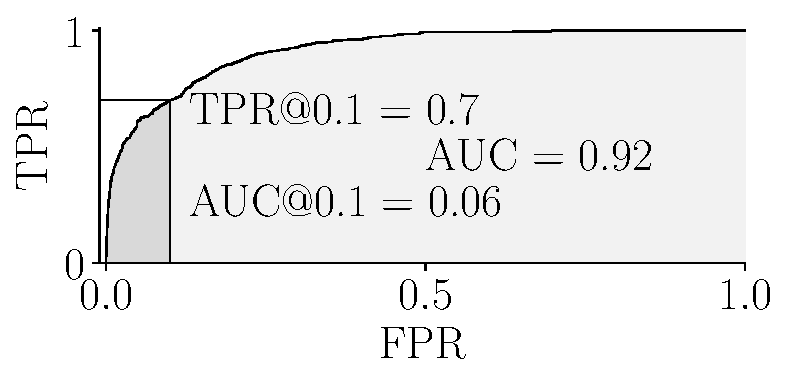
\includegraphics[width=\textwidth]{data/chapter_intro/roc_example.pdf}
	\caption{ROC curve}
	\label{fig:roc_example}
\end{subfigure}
\hfill
\begin{subfigure}[b]{0.45\textwidth}
	\centering
	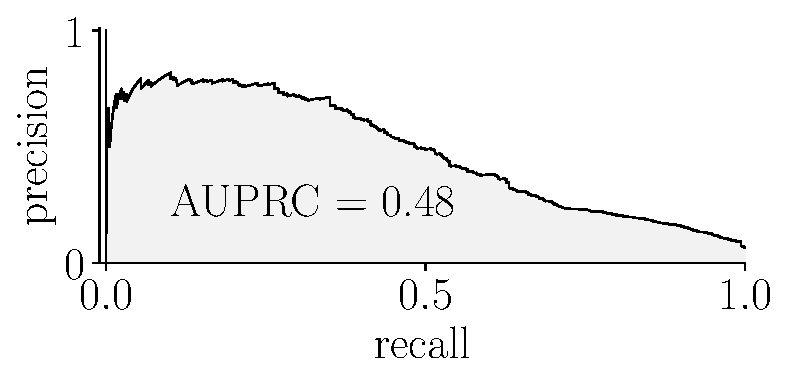
\includegraphics[width=\textwidth]{data/chapter_intro/prc_example.pdf}
	\caption{PR curve}
	 \label{fig:prc_example}
\end{subfigure}
\caption{An example of an ROC curve and the derived measures based on FPR=0.1. AUC is the whole shaded area under the ROC curve. The darker shading corresponds to AUC@0.1. On the left, the PR curve of the same detector is shown.}
\label{fig:ROC}
\end{figure}

\subsubsection{AUPRC}
The Area Under the Precision--Recall Curve is very similar to AUC, as it is given by computing the \textbf{precision} $\text{PREC}(\tau)=\frac{\text{tp}}{\text{tp + fp}}(\tau)$ and recall for different values of classification threshold $\tau$ and then integrating the area under the resulting curve. A PR curve has at most as many unique recall values as positive samples in the dataset. This is problematic for anomaly detection, where the number of anomalies is low, which leads to a very sparse estimate of the true PR curve. In fact, using the same trained anomaly detector and changing the contamination rate of a testing dataset produces different AUPRC results, which then makes any analysis based on AUPRC useless when the true contamination rate is unknown. Furthermore, a correct PR curve lacks a universal starting point, unlike an ROC curve, because precision is undefined for zero recall, making the computation and normalization of the area under the PR curve and the comparison between datasets even more complicated. It is still a metric that is reported very often besides the AUC.

\subsubsection{Areas of low TPR}
The two already mentioned metrics put the same weight on all areas on the x-axis. This might not be always ideal for the purposes of anomaly detection, as low FPR areas might be more interesting -- after all, when reporting detected anomalies for a manual check, there is always a limit on how many samples can be realistically processed. A performance measure popular among practitioners is \textbf{\tpra}, which is simply the true positive rate evaluated at a given false positive rate $\alpha \in [0,1]$. This measure can be easily read from an ROC curve. In practice, it is necessary to interpolate the ROC curve since FPR has discrete values, especially for datasets with a small number of samples. 

Another alternative to AUC is the partial AUC, or \textbf{\auca}, which is the area under the ROC curve calculated only up to some value of false positive rate $\alpha \in [0,1]$
\begin{equation} \label{eq:auc_alpha}
    \text{AUC@}\alpha = \int_0^{\alpha}\text{TPR}(\text{FPR})d\text{FPR}.
    \end{equation}    
Numerically, it is again important to interpolate the ROC curve for a given $\alpha$ before computing the integral. In Fig.~\ref{fig:ROC}, AUC@0.1 corresponds to the darker gray region. \auca\ can be easily normalized by dividing by the chosen $\alpha$, in which case the best detector has $\auca = 1$ similarly to AUC.

\subsubsection{Volume of decision region}
\begin{figure}
\centering
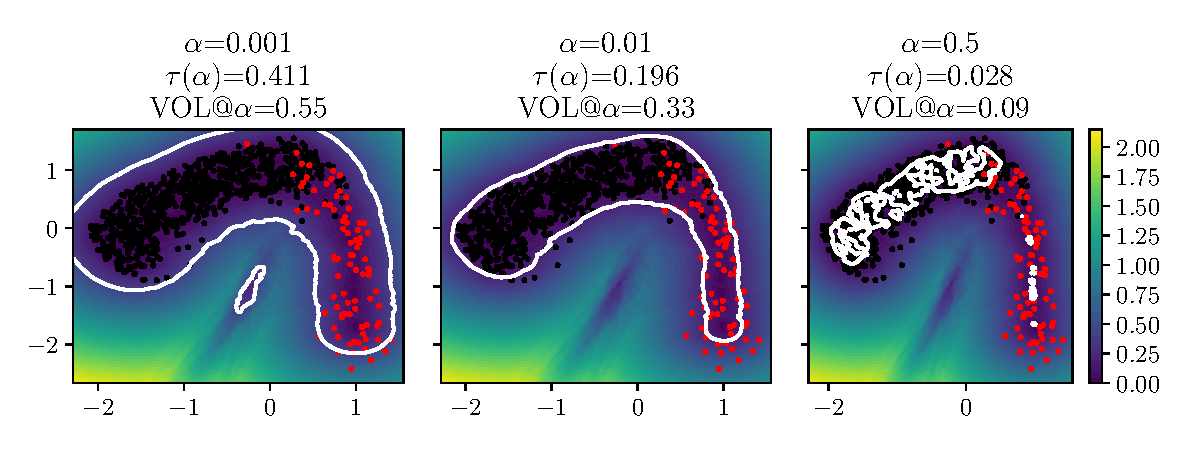
\includegraphics[scale=0.8]{data/chapter_intro/fig_vol_example.pdf}
\caption{An example of a detector and the decision region for differing values of FPR $\alpha$. The decision boundary is drawn as a white isoline at level $\tau(\alpha)$ with the estimated enclosed volume $\text{VOL@}\alpha$, black and red dots represent normal and anomalous samples in the training set. Clearly, smaller tolerance of false positives forces us to set a higher threshold which results in higher decision region volume.}
\label{fig:vol_example}
\end{figure}
All of the previous measures originate from the evaluation of the performance of binary classifiers. Since labeled anomalies are often difficult to obtain, a measure that does not require labels for its evaluation might be more useful and better describe behaviour on unknown samples. If the goal is to compare two models supposed to characterize the normal class, and with no other assumptions about the distribution of the anomalous class, it makes sense to choose the model enclosing the training data more tightly. This corresponds to calculating the volume inside the model's decision boundary in a similar fashion to \cite{clemenccon2013scoring}, where a theoretical justification is given. This decision boundary can be chosen to correspond to a certain level of false positive rate. We define the \textbf{volume of decision region} as
\begin{equation}
  \text{VOL}(\alpha) = \int_{\mathcal{X}} \mathds{1}_{\lbrace \vc{x} \in\mathcal{X}|s(\vc{x}) <= \tau\rbrace} \left( \vc{x} \right) d\vc{x}  \text{ s.t. } \text{FPR}(\tau)=\alpha,
\end{equation}
where $\mathcal{X}$ is the input space, $s(\vc{x})$ is an anomaly score, and $\alpha$ is a given false positive rate. In other words, $\text{VOL}(\alpha)$ is the volume of the subspace where the classifier returns "normal" answer with a false positive rate $\alpha$. An example of a model and its decision region for different values of $\alpha$ is shown in Fig.~\ref{fig:vol_example}. It should be noted that the idea of minizing the enclosed volume is native to some models, e.g. the SVDD model described in Sec.~\ref{sec:domain_methods}.

Computing the empirical $\text{VOL}(\alpha)$ in data space $\mathcal{X}$ requires first finding the threshold $\tau$ corresponding to the chosen FPR $\alpha$ and then integrating the volume which corresponds to the space enclosed by the isosurface where the anomaly score is equal to $\tau$. It is numerically estimated by Monte Carlo sampling~\cite{robert1999monte}. This comes with its downsides. Mainly, the number of samples required to cover $d$--dimensional sample space grows exponentially with $d$. This issue has been addressed in \cite{goix2016evaluate}, where the volume is computed multiple times for different subsampling of input features, however this does not seem to be optimal as it requires training a new model for each subset of features.


\section{Anomaly detectors taxonomy} \label{sec:taxonomy}
Anomaly detection methods are based on a wide range of paradigms. In this section we will follow the taxonomy outlined in publications~\cite{pimentel2014review, ruff2020unifying}, which divide shallow (not based on neural networks) and deep (based on neural networks) detectors into groups based on their common traits. Note that this taxonomy is tentative, and in fact some methods have traits common to multiple groups. Examples of methods will be given since their knowledge will be useful in the later chapters of this text, but the list is far from complete. For a complete overview of the landscape of anomaly detection methods, see the surveys~\cite{pimentel2014review, campos2016evaluation, goldstein2016comparative, moustafa2019holistic, kwon2019survey, fernandes2019comprehensive, wang2019progress, chalapathy2019deep,ruff2020unifying}.

\subsection{Probabilistic  methods} \label{sec:probabilistic_models}
Since we have defined anomaly detection as detecting samples that deviate from the normal distribution $P^+$, it is straightforward to try to model the distribution by modeling its probability distribution function (pdf). One of the simplest such methods is the Grubbs' test~\cite{grubbs1969procedures}, which assumes a Gaussian distribution of normal one-dimensional data and declares a sample to be anomalous if its distance from the mean is larger than some threshold (e.g. three standard deviations). Many such methods based on statistical tests have been proposed~\cite{barnett1994outliers}, but we will focus on advanced modeling probabilistic techniques.

\subsubsection{Shallow methods}
A \textbf{Mahalabonis distance} anomaly detector~\cite{laurikkala2000informal} builds a parametric estimate of a multivariate normal distribution by computing the mean $\vc{\mu} \in \mathbb{R}^d$ and covariance matrix $\Sigma \in \mathbb{R}^{d,d}$ of the training data. The anomaly score of a test point $\vc{x} \in \mathbb{R}^d$ is then
\begin{equation} \label{eq:mahalabonis_score}
	s(\vc{x}) =  (\vc{x} - \vc{\mu}) ^T \Sigma ^{-1} (\vc{x}-\vc{\mu}),
\end{equation}
which is equivalent to the evaluation of the negative log-likelihood under the Gaussian distribution. Even though this is one of the simplest and most non-robust methods, terms similar to~\eqref{eq:mahalabonis_score} will be encountered a lot in the remainder of this text.

Instead of limiting the model to a single-mode distribution, a mixture of $K$ distributions 
\begin{equation} \label{eq:mixture}
	p(\vc{x}) = \sum_{k=1}^K p(k) p(\vc{x}|k), p(k) \in [0,1], \sum_{k=1}^K p(k) = 1,
\end{equation}
can be estimated instead, where $p(k)$ is the prior probability of the $k$-th component. \textbf{Gaussian Mixture Models} (GMMs) have been used for anomaly detection in~\cite{roberts1994probabilistic,mahadevan2010anomaly}. There, we assume that $p(\vc{x}|k)$ are Gaussian distribution densities and their parameters are estimated using the EM algorithm~\cite{dempster1977maximum} or via Variational Bayes~\cite{bishop2006pattern}. The term $-\log p(\vc{x})$ is usually used as the anomaly score, although sometimes the maximum of the Mahalabonis distance~\eqref{eq:mahalabonis_score} over the $K$ components is used instead. However, the viable usecases for a GMM anomaly detector are limited, mainly due to the need to compute and invert the covariance matrix, which is $O(d^3)$ in the size of the input space $d$ (when the full covariance matrix is estimated). See Fig.~\ref{fig:gmm_examples}, where the same anomaly detection problem is solved by GMMs with different number of components. Even though the AUC score is already perfect for 2 components, the difficult shape of the normal data needs more components than that to be fully covered.

Time series data anomaly detection was approached with the use of \textbf{Autoregressive Integrated Moving Average} (ARIMA) models in~\cite{roberts1994probabilistic,hoare2002line}, or using a \textbf{Hidden Markov Model} (HMM) in~\cite{yeung2003host,zhang2003new}. Both approaches offer predictions for future states of an observed system, and the anomaly score is the difference between the prediction and the actual state of the system. The problems to which these methods can be applied are encountered in medicine or computer network intrusion detection.

All the previous were examples of parametric models, where a set of parameters $\vc{\theta}$ is directly estimated. Opposed to these are non-parametric models, which are less restricting  -- e.g. they do not assume any (normal, Poisson, ...) distribution -- instead, they build a parameter-free model of the normal data. \textbf{Kernel density estimation} (KDE) method~\cite{parzen1962estimation}, which estimates an unknown univariate probability density function by an empirical estimate
\begin{equation} \label{eq:kde}
	\hat{p}(x) = \frac{1}{hn} \sum_{i=1}^n k_f \left( \frac{x-x_i}{h} \right), x_i \in X
\end{equation}
where $X = \lbrace x_1, x_2, \ldots, x_n \rbrace$ is the training dataset of $n$ samples, $h \in \mathbb{R}^+$ is a bandwidth parameter, and $k_f:\mathbb{R} \rightarrow \mathbb{R}^+$ is a kernel function (uniform, triangular, normal, etc.). KDE has been used under the name Parzen window estimate e.g. in~\cite{tarassenko1995novelty,yeung2002parzen}, where $-\ln \hat{p}(x)$ is used to score anomalies. \textbf{Histogram-based Outlier Score} (HBOS) is a method~\cite{goldstein2012histogram} for anomaly detection on multivariate data $\vc{x} \in \mathbb{R}^d$. It computes normalized histograms for each feature $x_j$ independently. Then the anomaly score for an unlabeled sample $\vc{x}$ is
\begin{equation} \label{eq:hbos}
	s(\vc{x}) =  -\sum_{j=1}^d \ln \tilde{p}_j(\vc{x})
\end{equation}
where $\tilde{p}_j(\vc{x})$ is the height of the bin in which $x_j$ is located. The main advantage of this method in comparison with e.g. distance-based is the relative computational simplicity. In the \textbf{Lightweight Online Detector of Anomalies} (LODA)~\cite{pevny2016loda}, an ensemble of one-dimensional histograms is used in a space of diversified projection vectors. The anomaly score is then an average of the logarithm of probabilities estimated from the histograms on individual projection vectors. Due to its simplicity and computational efficiency, it is popular in settings with high volumes of data and potentially missing input values.

\begin{figure}
\begin{centering}
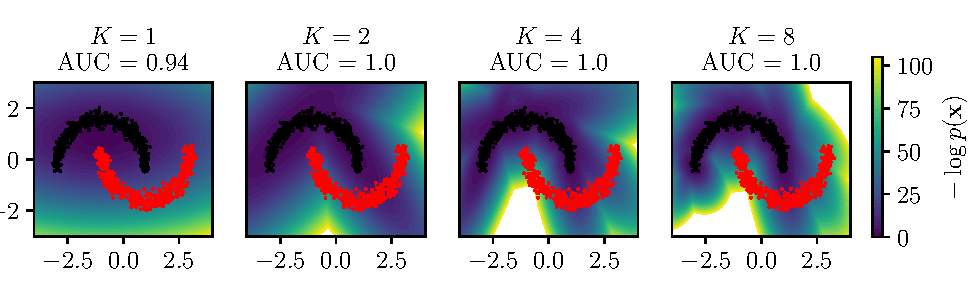
\includegraphics[scale=0.98]{data/chapter_intro/gmm_examples.pdf}
\end{centering}
\caption{The \textit{two bananas} dataset consists of two clusters of points. The black points are considered to be normal and the red are considered to be anomalies. The dataset is useful for introducing behaviour of anomaly detectors, because as an anomaly detection problem, it cannot be solved by a linear separation of the two groups of points. Here, GMM models with a varying number of components $K$ are fitted to the normal datapoints. The contours of the anomaly score based on~\eqref{eq:mixture} are shown together with the AUC computed with respect to the anomalous datapoints.}
\label{fig:gmm_examples}
\end{figure}

\subsubsection{Deep methods}
The recent advent of neural networks has given rise to many novel methods that are more capable of handling high-dimensional datasets that would be otherwise extremely difficult to handle. A mixture model was used in the \textbf{DAGMM} method~\cite{zong2018deep}, where a neural network creates a low-dimensional latent representation $\vc{z}$ from an input $\vc{x}$. The GMM and its parameters are then estimated in the latent space, again via a neural network, which enables online learning of the whole model together.

\textbf{Energy based models} (EBMs) use the energy function $E_{\vc{\theta}}(\vc{x})$ to approximate the density as
\begin{equation} \label{eq:ebm}
	p_{\vc{\theta}}(\vc{x}) =  \frac{1}{Z(\vc{\theta})} \exp (- E_{\vc{\theta}}(\vc{x})),
\end{equation}
where $Z(\vc{\theta})$ is the partition function parametrized by $\vc{\theta}$ to ensure proper normalization of $p_{\vc{\theta}}(\vc{x})$. Although the partition function usually cannot be directly computed, an EBM can still be trained via gradient descent coupled with Markov Chain Monte Carlo estimation~\cite{hinton2002training}, which is however also the reason for its ineffectiveness relative to more novel approaches, as the MCMC is computationally costly. The anomaly score is then the energy function $E_{\vc{\theta}}(\vc{x})$. Although the direct use of the early examples of EBMs such as \textbf{Deep Belief Networks}~\cite{hinton2006fast} and \textbf{Deep Boltzmann Machines}~\cite{salakhutdinov2010efficient} was impractical for anomaly detection, they were eventually refined and successfully used on anomaly detection benchmarks in~\cite{zhai2016deep}. 

Finally, the most recent advancements in anomaly detection were achieved with the use of deep generative models that model the distribution of the data via a generative process, where it is assumed that the data is generated from a hidden latent variable. \textbf{Flow models}~\cite{dinh2014nice}, \textbf{Variational autoencoders}~\cite{kingma2013vae} and \textbf{Generative Adversarial Networks}~\cite{goodfellow2014gan}  will be described in greater detail in Chapter~\ref{sec:chapter_survey}.

\subsection{Distance-based methods} \label{sec:distance_methods}
Instead of modeling the probability distribution of the normal data, distance-based anomaly detectors use heuristics that compute a well-defined similarity measure between two data points. One of the simplest such models is the \textbf{k-Nearest Neighbor} (kNN)~\cite{ramaswamy2000efficient} model where the anomaly score of a sample is based on its proximity to its $k$--nearest neighbours from the training dataset. Different proximity measures are described in~\cite{harmeling2006outliers}, where 
the Euclidean distance is used as the similarity measure and the set $X_{k}(\vc{x})$ is defined as the set of $k$-nearest neighbors of $\vc{x}$ from a training dataset $X = \lbrace \vc{x}_1, \vc{x}_2, \ldots, \vc{x}_n \rbrace \subset \mathbb{R}^d$.
\begin{itemize}
	\item $\kappa(\vc{x})$: the anomaly score is the distance between $\vc{x}$ and its $k$th-nearest neighbor,
	\begin{equation} \label{eq:knn_kappa}
		s_{\kappa}(\vc{x}) =  \max_{\vc{x}_i \in X_k(\vc{x})} \vert \vert \vc{x} - \vc{x}_i \vert \vert_2,
	\end{equation}
	\item $\gamma(\vc{x})$: the anomaly score is the average distance of $\vc{x}$ to its $k$-nearest neighbors, 
	\begin{equation} \label{eq:knn_gamma}
		s_{\gamma}(\vc{x}) =  \frac{1}{k} \sum_{\vc{x}_i \in X_k(x)} \vert \vert \vc{x} - \vc{x}_i \vert \vert_2,
	\end{equation}
	\item $\delta(\vc{x})$: the anomaly score is the length of the mean of the vectors pointing from $\vc{x}$ to its $k$-nearest neighbours,
	\begin{equation} \label{eq:knn_delta}
		s_{\delta}(\vc{x}) =  \left| \left| \frac{1}{k} \sum_{\vc{x}_i \in X_k(x)} (\vc{x}_i - \vc{x}) \right| \right|_2.
	\end{equation}
\end{itemize}
All these definitions presume that normal data lie in concentrated regions of the data space $\mathcal{X}$, according to~\eqref{eq:normal_concentration}, while anomalies lie outside of them. The kNN anomaly detector is very popular thanks to its simplicity and good performance~\cite{campos2016evaluation}. See Fig.~\ref{fig:knn_examples}, where low values of $k$ result in a very local behaviour of the model, which is suitable for this problem. The biggest disadvantage of the model is the computational cost. Even though there is no actual training procedure, the prediction complexity is $O(ndk)$. This can be ameliorated by the construction of a $k$-d tree~\cite{bentley1975multidimensional}, which partitions the space of the training data to speed-up prediction, or using GPU-based similarity search techniques such as~\cite{johnson2019billion}. Other methods, such as \textbf{REPEN}~\cite{pangLearningRepresentationsUltrahighdimensional2018}, use the kNN detector trained on low-dimensional representations of otherwise high-dimensional data produced by a deep neural network.

The \textbf{Local Outlier Factor} (LOF) algorithm~\cite{breunig2000lof} is based on comparing the local density of a sample $\vc{x}$ with the local density of its $k$--nearest neighbours. To correctly describe the way in which the density is defined and the anomaly score is computed, we use the formula~\eqref{eq:knn_kappa}. Then we define the \textit{local reachability density} as 
\begin{equation}
  \text{LRD}_k(\vc{x})=\frac{|X_k(\vc{x})|}{\sum_{\vc{x}_i\in X_k(x)} \max \lbrace s_{\kappa}(\vc{x}), \vert \vert \vc{x} - \vc{x}_i \vert \vert_2 \rbrace }.
\end{equation}
Since this is basically the inverse of an average distance between $\vc{x}$ and its neighbours, the closer the neighbours are to $\vc{x}$, the higher this approximation of local density is. Finally, anomaly score of $\vc{x}$ is given by comparing the $\text{LRD}_k$ of $\vc{x}$ and its neighbours 
\begin{equation}
  s_{\text{LOF}}(\vc{x})=\frac{\sum_{\vc{x}_i\in X_k(\vc{x})} \text{LRD}_k(\vc{x}_i)}{\text{LRD}_k(\vc{x}) |X_k(\vc{x})|}.
\end{equation}
The rationale behind the formula is that if the local density of the neighbours is higher or the local density of $\vc{x}$ is lower then it is more likely for $\vc{x}$ to be an anomaly. This method however does not scale well in number of training samples, as its complexity is even greater than that of a simple kNN detector. Similar methods to LOF are the \textbf{connectivity--based outlier factor} (COF)\,\cite{tang2002enhancing} or \textbf{clustering--based local outlier factor} (CBLOF)\,\cite{he2003discovering}.

\begin{figure}
\begin{centering}
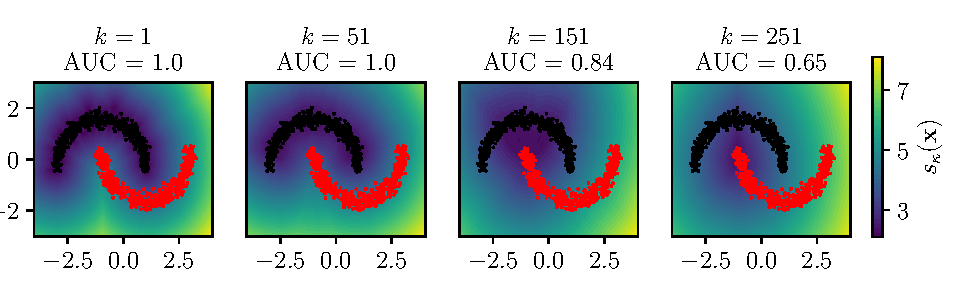
\includegraphics[scale=0.98]{data/chapter_intro/knn_examples.pdf}
\end{centering}
\caption{K-nearest neighbor detectors on the \textit{two bananas dataset}. The contours of the score~\eqref{eq:knn_kappa} are shown for different values of $k$ together with the resulting AUC.}
\label{fig:knn_examples}
\end{figure}

A different approach is taken by the \textbf{isolation forest }(IF) model~\cite{liu2008isolation} where an ensemble of $N_t$ isolation trees is constructed for the whole dataset. Isolation trees are constructed in such a way as to isolate each individual datapoint from the rest of the dataset using consecutive splits on different features. It is presumed that an anomaly can be isolated using a smaller number of splits and therefore it lies on a branch closer to the root of the tree. The anomaly score is then based on the number of splits of a sample averaged over multiple randomly initialized trees in the ensemble. A method similar to IF is the \textbf{Partial Identification Forest} (PIDForest)~\cite{gopalanPIDForestAnomalyDetection2019}, which uses a more informed way of choosing the data features for split, favouring the more informative features.

In \textbf{Angle-Based Outlier Detection} (ABOD)~\cite{kriegel2008angle} presumes that outliers lie far from clusters of normal data, therefore the viewing angle that covers a cluster of normal datapoints when "looking" at it from a sample $x$ is smaller when $x$ is anomalous. More concretely, the method computes the angles between $x$ and all pairs of points in the training dataset, and the anomaly score is inversely proportional to the variance of these angles -- the more varied the angles are, the more likely $x$ is close to some cluster of normal data and the anomaly score is thus lower. In the original paper, the method is lauded for the lack of hyperparameters that need to be tuned and the ability to operate in high-dimensional data spaces. However, in the experiments in Chapter~\ref{sec:chapter_comparison}, it proves to be the method with one of the slowest prediction times.

\subsection{Domain-based  methods} \label{sec:domain_methods}
Some anomaly detectors divide the data space into a normal and anomalous subspace (domain). In~\cite{ruff2020unifying}, these are labeled as domain-based, and we will follow that distinction here.

\subsubsection{Shallow methods}
In domain-based models, the data space is partitioned into subspaces by a decision boundary. Instead of estimating the density of the whole training dataset, they only consider a few samples from it, which are called \textit{support vectors}, and which are used to define the decision boundary. A very simple example is an anomaly detector which, for a training set $X = \lbrace \vc{x}_1, \vc{x}_2, \ldots, \vc{x}_n \rbrace \subset \mathbb{R}^d$, constructs a hypersphere with center $\vc{c} \in \mathbb{R}^d$ and radius $R>0$ that encloses the training data. It is found by solving the objective
\begin{alignat}{1}
\mathclap{
	\begin{aligned}
	\min_{R,\vc{c},\vc{\xi}} R^2 & + \frac{1}{\nu n}\sum_{i=1}^n \xi_i \\
	\text{s.t.} \vert \vert \vc{x}_i - \vc{c} \vert \vert_2^2 & \leq R^2 + \xi_i, \xi_i \geq 0, \forall i
\end{aligned}
} \label{eq:hypersphere}
\end{alignat}
where $\xi_i$ are slack variables that allow some data points to lie outside of the hypersphere. The ratio of the maximum number of outliers is controlled by the variable $\nu \in (0,1]$, which is at the same time a lower bound on the number of support vectors, which are samples $\vc{x}_i$ that lie exactly on the boundary of the hypersphere. The solution to~\eqref{eq:hypersphere} is given by solving the dual problem. Notice that a simple criterion $\vert \vert \vc{x} - \vc{c} \vert \vert_2^2  \leq R^2$ already gives a decision whether the point $\vc{x}$ is already inside the sphere. To convert this to a continuous anomaly score, we can compute the distance of $\vc{x}$ from the boundary
\begin{equation} \label{eq:hypersphere_score}
	s(\vc{x}) = \vert \vert \vc{x} - \vc{c} \vert \vert_2^2 - R^2
\end{equation}
which is negative for points inside and positive for points outside the hypersphere.

Abstracting the above, one can use \textit{kernel functions}~\cite{shawe2004kernel} to move the problem~\eqref{eq:hypersphere} from the original input space to a transformed kernel space. The kernel is a function $k_f:\mathbb{R}^d \times \mathbb{R}^d \rightarrow \mathbb{R}$, with which we associate a \textit{feature map} $\Phi: \mathbb{R}^d \rightarrow \mathcal{F}_k$ such that the relation defined by the inner product $k_f(\vc{x},\vc{y})=\langle \Phi(\vc{x}), \Phi(\vc{y}) \rangle$ is true for all $\vc{x},\vc{y}$. The space $\mathcal{F}_k$ is a reproducing kernel Hilbert space and we choose the kernel in such a way that its dimensionality is higher than $d$. This is the basis for the \textbf{Support Vector Data Descriptor} (SVDD) anomaly detector, where the inequality condition in~\eqref{eq:hypersphere_score} is replaced by $\vert \vert \Phi(\vc{x}_i) - \vc{c} \vert \vert_2^2 \leq R^2 + \xi_i$. By solving the problem in a space of higher dimensionality, it is possible to find a decision boundary (hypersphere) for datapoints that would otherwise not be separable in the original space. In comparison, the \textbf{One-Class Support Vector Machine} (OCSVM)~\cite{scholkopf2001estimating} does not construct a hypersphere, but instead aims to find a separating hyperplane in the kernel space. See Fig.~\ref{fig:ocsvm_examples} for a demonstration of the OCSVM model on our toy dataset.  Unlike in traditional SVM~\cite{cortes1995support}, which is used to separate two classes in a binary classification problem, OCSVM instead aims to find a hyperplane that maximizes the separation of the majority of the training data from the origin in the kernel space. The anomaly score of an OCSVM detector is, similarly to~\eqref{eq:hypersphere_score}, the distance from the separating hyperplane. Apart from $\nu$, a very important hyperparameter of the model is the kernel scale parameter $\gamma_{\text{OCSVM}}$. Many variants of both of the presented approaches were introduced over the years, such as \textbf{Minimum Volume Ellipsoid}~\cite{van2009minimum}, \textbf{Multi-sphere SVDD}~\cite{gornitz2017support} or \textbf{Bayesian Data Description}~\cite{ghasemi2012bayesian}.

\begin{figure}
\begin{centering}
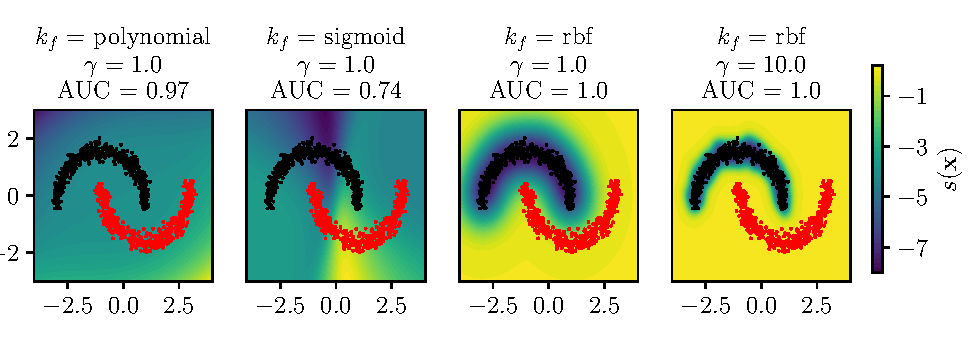
\includegraphics[scale=0.98]{data/chapter_intro/ocsvm_examples.pdf}
\end{centering}
\caption{OCSVM detectors with different kernel functions and kernel width parameter $\gamma$ values on the \textit{two bananas dataset}. The contours of the score~\eqref{eq:hypersphere_score} together with the resulting AUC. Although the use of both the polynomial and sigmoid kernels results in a relatively good AUC value, the anomaly score contours reveal that the model would fail if the anomalies would be placed slightly differently. On the other hand, the tight fit of the training data with the \textit{radial basis function} (rbf) is proportional to the kernel width.}
\label{fig:ocsvm_examples}
\end{figure}

\subsubsection{Deep methods}
Instead of choosing a kernel and its parameters manually, one can instead parametrize the feature maps $\Phi$ using neural networks and train them using standard gradient descent techniques, or use pretrained networks from related tasks. This is the basis for deep OCSVM methods such as \textbf{One-class Neural Network} (OCNN)~\cite{chalapathy2018anomaly} or~\cite{erfani2016high}, or methods based on the SVDD formulation~\cite{ghafoori2020deep}. In \textbf{Deep SVDD} (DSVDD)~\cite{ruff2018deep}, the objective~\eqref{eq:hypersphere} is reformulated without the slack variables $\xi_i$, which means that the hypersphere is expected to enclose all datapoints in the training dataset. This simplification leads to faster convergence and yet still proves to be an effective anomaly detector. However, all the deep methods have a basic flaw. Without any further restrictions, the solution $\Phi(\vc{x}) = \vc{c}$ is valid but does not provide a useful detector. This behaviour is called the \textit{feature map collapse}. In order to prevent this, many techniques such as freezing the neural networks that provide the feature map, architectural choices or using adversarial learning are used (for an extensive list of possibilities, see~\cite{ruff2020unifying}).

\subsubsection{Training with negative examples}
Although we have stated in Sec.~\ref{sec:ad_definition} that anomaly detection methods do not usually consider the distribution of anomalies $P^-$, there are some approaches that do. These still fall under the domain-based category of anomaly detectors, as they are mostly constructed as binary classifiers that divide the input space into subspaces where either the anomalous or normal class is expected. In the simplest case~\cite{steinwart2005classification}, $P^-$ is assumed to be uniform and a supervised classifier is trained using anomalies sampled from a hypercube centered around the normal data. This approach however suffers from the curse of dimensionality and saturating the hypercube in high-dimensional spaces is computationally infeasible, especially for image data. Some attempts for a more efficient sampling have been proposed, such as sampling based on local density esimation~\cite{fan2004using}. In \textbf{outlier exposure}~\cite{hendrycksDeepAnomalyDetection2019} techniques, a large auxiliary dataset, that is somehow related to normal data, is used to improve the generalization properties of a deep anomaly detector. For example, if the normal class consists of images of birds, it might be useful to train the detector to recognize normal data from images containing other animals, even though this auxiliary dataset may contain animal classes that will not be encountered as anomalies in test/production environment. It has been shown to be an effective technique in~\cite{hendrycks2019using}.  

Outlier exposure is a form of \textbf{weak supervision}~\cite{zhou2018brief}, which is a more general term covering the approach to learning with imperfectly labeled anomaly samples. In~\cite{ruff2019deep,liznerski2020explainable} it is shown that using even a few labeled examples of anomalies can dramatically improve the detection performance. It is however important to robustify the model in order to be able to generalize to the types of anomalies not present in the labeled training dataset. These techniques can help in \textbf{active learning} in anomaly detection~\cite{abe2006outlier}, where the anomaly detector sends queries to its operator, asking for the most informative/relevant samples to be manually labeled. It is stated in~\cite{ruff2020unifying} that weak supervision is essential for potential breakthroughs in anomaly detection, which is the motivation for the method proposed in Chapter~\ref{sec:chapter_sgvaegan}.

Another paradigm where the model is trained in the presence of additional data is \textbf{self-supervision}~\cite{kolesnikov2019revisiting}, where the model solves an auxiliary task, such as prediction of transformations applied to the image~\cite{chen2020simple}. The important distinction between this approach and outlier exposure is that the transformed data is obtained from the normal training dataset by applying random translations, scalings, rotations, etc. Transforming the data in a controlled manner, the anomaly detector is then a multiclass classifier that predicts the correct transformation applied to the data. The anomaly score of such a model is then based on the softmax activations in the output layer -- if the prediction uncertainty is high, the scored sample is more likely to be an anomaly. This was very successfully used in the \textbf{Geometric Transformations} (GT)~\cite{golan2018deep} anomaly detector. Furthermore, the \textbf{GOAD} method~\cite{bergman2020classification} extends this approach to non-image data.

\subsection{Reconstruction-based methods} \label{sec:reconstruction_models}
One of the most popular approaches to anomaly detection is to build a model that learns to reconstruct input samples. When this model is trained on normal data and learns to reconstruct them well, it is expected that it will be able to identify anomalies by failing to reconstruct them properly, since they have properties unseen by the model at training time. To formalize this, a reconstruction-based anomaly detector consists of an \textit{encoder}, which is a mapping $e_{\vc{\phi}}:\mathcal{X} \rightarrow \mathcal{Z}$, and a \textit{decoder} $g_{\vc{\theta}}: \mathcal{Z} \rightarrow \mathcal{X}$. Here, $\mathcal{X} \subset \mathbb{R}^d$ is the input space, $\mathcal{Z} \subset \mathbb{R}^h$ is a so called \textit{latent} space and $\vc{\phi},\vc{\theta}$ are parameters. A \textit{latent representation} or \textit{encoding} of a sample $\vc{x}$ is $z = e_{\vc{\phi}}(\vc{x})$. Reconstruction-based methods then try to match the original sample $\vc{x}$ with its reconstruction $\vc{x}' = g_{\vc{\theta}}(\vc{z})=g_{\vc{\theta}}(e_{\vc{\phi}}(\vc{x}))$. This is done by finding such parameters $\vc{\phi}, \vc{\theta}$ as to minimize the reconstruction objective
\begin{equation} \label{eq:reconstruction_objective}
	\min_{\vc{\phi}, \vc{\theta}} \vert \vert \vc{x} - g_{\vc{\theta}}(e_{\vc{\phi}}(\vc{x})) \vert \vert_2^2 + \mathcal{R},
\end{equation}
where $\mathcal{R}$ is a regularization term. Some sort of regularization is needed in order to prevent the decoding function $(g_{\vc{\theta}} \circ e_{\vc{\phi}})(\vc{x})$ to become an identity function, in which case the detector would be useless. The anomaly score of reconstruction-based methods is the \textit{reconstruction error}
\begin{equation} \label{eq:reconstruction_error}
	s(\vc{x}) = \vert \vert x - g_{\vc{\theta}}(e_{\vc{\phi}}(\vc{x})) \vert \vert_2^2.
\end{equation}


The \textbf{Principal Component Analysis} (PCA)~\cite{shyu2003novel,aggarwal2015outlier}, although not originally developed for this purpose, is an example of a reconstruction anomaly detection method. It is assumed that the normal data lie on a lower-dimensional manifold in the data space, which is an assumption also used in other methods. This means that theoretically, they can be represented by a transformation into a lower dimensional latent space, and the eventual differences between the reconstructions from the latent back to the data space and the original samples are only due to noise that is present in the data, and therefore the latent representation contains all the relevant information of a sample. PCA seeks to represent the data by finding an orthonormal basis $W \in \mathbb{R}^{h,d}$ that maximizes the empirical variance of the data $X= \lbrace \vc{x}_1, \vc{x}_2, \ldots, \vc{x}_n \rbrace \subset \mathbb{R}^d$. The original objective of PCA can be reformulated with~\eqref{eq:reconstruction_objective} in mind, which yields 
\begin{equation} \label{eq:pca}
	\max_W \sum_{i=1}^n \vert \vert \vc{x}_i -  W^TW \vc{x}_i \vert \vert_2^2, \text{s.t.} WW^T = I.
\end{equation}
Thus, this means $\vc{z} = e_{\vc{\phi}}(\vc{x}) = W \vc{x} \in \mathbb{R}^h$ is the encoding represented by the first $h$ \textit{principal components}, while the decoder is $g_{\vc{\theta}}(\vc{z}) = W^T\vc{z}$. The solution to~\eqref{eq:pca} is obtained by collecting the first $h$ eigenvectors of the covariance matrix of the training data, e.g. through its eigendecomposition, or by computing the \textit{singular value decomposition} of the data matrix. Like in the domain-based methods in Sec.~\ref{sec:domain_methods}, some of the restrictions imposed by the linear formulation of classical PCA are circumvented by using a \textbf{kernel PCA} (kPCA)~\cite{scholkopf1998nonlinear}, where $x$ is replaced by its nonlinear transformation $\Phi(\vc{x})$. This was used for anomaly detection e.g. in~\cite{xiao2013l1}.

\begin{figure}
\begin{centering}
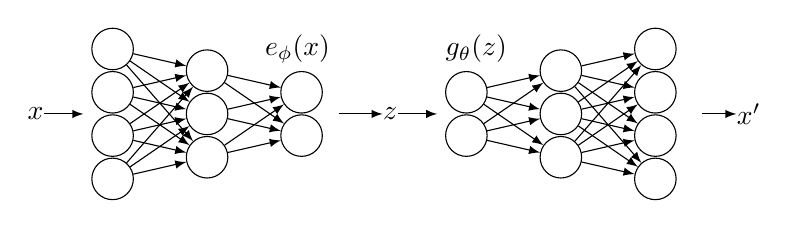
\begin{tikzpicture}
  \node[const]                               (x) {$\vc{x}$};
  \node[const, right = 0.5cm of x]           (xin) {};
  % encoder in
  \node[latent, right = 0.6cm of x, yshift = 0.825cm] (E11) {};
  \node[latent, right = 0.6cm of x, yshift = 0.275cm] (E12) {};
  \node[latent, right = 0.6cm of x, yshift = -0.275cm] (E13) {};
  \node[latent, right = 0.6cm of x, yshift = -0.825cm] (E14) {};
  % encoder hidden
  \node[latent, right = 1.8cm of x, yshift = 0.55cm] (E21) {};
  \node[latent, right = 1.8cm of x, yshift = 0cm] (E22) {};
  \node[latent, right = 1.8cm of x, yshift = -0.55cm] (E23) {};
  % encoder out
  \node[latent, right = 3cm of x, yshift = 0.275cm] (E31) {};
  \node[latent, right = 3cm of x, yshift = -0.275cm] (E32) {};
  % encoder tag
  \node[const, right = 2.8cm of x, yshift = 0.825cm] (E) {$e_{\vc{\phi}}(\vc{x})$};
  % code
  \node[const, right = 4.3cm of x]           (z) {$\vc{z}$};
  \node[const, right = -0.8cm of z]           (zout) {};       
  \node[const, right = 0.5cm of z]           (zin) {};
  % decoder in
  \node[latent, right = 0.6cm of z, yshift = 0.275cm] (D11) {};
  \node[latent, right = 0.6cm of z, yshift = -0.275cm] (D12) {};
  % decoder hidden
  \node[latent, right = 1.8cm of z, yshift = 0.55cm] (D21) {};
  \node[latent, right = 1.8cm of z, yshift = 0cm] (D22) {};
  \node[latent, right = 1.8cm of z, yshift = -0.55cm] (D23) {};
  % decoder out
  \node[latent, right = 3cm of z, yshift = 0.825cm] (D31) {};
  \node[latent, right = 3cm of z, yshift = 0.275cm] (D32) {};
  \node[latent, right = 3cm of z, yshift = -0.275cm] (D33) {};
  \node[latent, right = 3cm of z, yshift = -0.825cm] (D34) {};
  % xhat
  \node[const, right = 4.3cm of z]           (xhat) {$\vc{x}'$};
  \node[const, right = -0.8cm of xhat]       (xhatout) {};       
  % decoder tag
  \node[const, right = 0.6cm of z, yshift = 0.825cm] (D) {$g_{\vc{\theta}}(\vc{z})$};
  

  % edges
  \nedge {x} {xin}
  % encoder 
  \nedge {E11, E12, E13, E14} {E21, E22, E23}
  \nedge {E21, E22, E23} {E31, E32}
  % latent
  \nedge {zout} {z}
  \nedge {z} {zin}
  % decoder
  \nedge {D11, D12} {D21, D22, D23}
  \nedge {D21, D22, D23} {D31, D32, D33, D34} 
  %xhat
  \nedge {xhatout} {xhat}

  % encoder plate
%  \plate {E} {(E11)(E14)(E32)} {};
\end{tikzpicture}

\par\end{centering}
\centering{}\caption{An example of an autoencoder consisting of fully connected layers. The latent code $\vc{z}\in\mathbb{R}^{2}$ is computed by propagating the input $\vc{x} \in\mathbb{R}^{4}$ through the encoder $e_{\vc{\phi}}(\vc{x})$ and then used to produce the reconstruction $\vc{x}'\in\mathbb{R}^{4}$ via the decoder $g_{\vc{\theta}}(\vc{z})$.}
\label{fig:ae}
\end{figure}

\begin{figure}
\begin{centering}
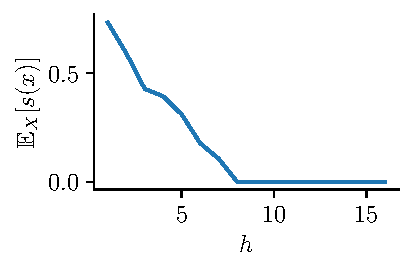
\includegraphics[scale=1.0]{data/chapter_intro/ae_reconstruction}\caption{The figure demonstrates the ability of an autoencoder to reconstruct data. The dimension $h$ of the latent space $\mathcal{Z}$ is on the x--axis, while the average reconstruction error~\eqref{eq:reconstruction_error} over the whole dataset is on the y--axis. Note that although the artificial dataset is 16--dimensional, it only contains 8 non--correlated dimensions while the remaining are a linear combination of them, which makes the data lie on an 8-dimensional manifold. This results in the error dropping to zero for $h>=8$ where the model is able to disentangle the correlations and learn the identity function.}
\label{fig:ae_reconstruction}
\par\end{centering}
\end{figure}

An \textbf{autoencoder} (AE)~\cite{kramer1991nonlinear} is in its basic principle a nonlinear PCA, where the encoder $e_{\vc{\phi}}$ and decoder $g_{\vc{\theta}}$ are neural networks and the parameters $\vc{\phi},\vc{\theta}$ are the trainable weights of these networks. The nonlinearity comes from the use of nonlinear activation functions between the individual layers of the neural networks. An example of an AE network is in Fig.~\ref{fig:ae}.  To find the weights of the neural networks, the reconstruction error ~\eqref{eq:reconstruction_error} is minimized 
\begin{equation} \label{eq:ae_objective}
\mathcal{L}_{\text{AE}}(\vc{x},\vc{\phi},\vc{\theta}) = \vert \vert \vc{x} - g_{\vc{\theta}}(e_{\vc{\phi}}(\vc{x})) \vert \vert_2^2
\end{equation}
with respect to $\vc{\phi},\vc{\theta}$ using a gradient descent technique, such as ADAM~\cite{kingma2014adam} or AMSGrad~\cite{reddi2019convergence}, which use backpropagation~\cite{werbos1982applications}. Note that the explicit regularization term $\mathcal{R}$ from~\eqref{eq:reconstruction_objective} here is omitted and instead, the regularization is enforced by creating a \textit{bottleneck} $h < d$, which again forces the model to find the optimal representation of data on a manifold of the data space, as is demonstrated in Fig.~\ref{fig:ae}. Other types of regularizations include sparse autoencoders~\cite{deng2013sparse}, where sparsity of encodings is enforced, or denoising autoencoders~\cite{lu2013speech}, which reconstruct samples with added artificial noise. The process of training an autoencoder is described in Alg.~\ref{alg:ae_train}. Note that the space if inputs $\mathcal{X}$ might be an euclidean space $\mathbb{R}^d$ for tabular data, while RGB images are usually represented by three-dimensional tensors of width $W$ and height $H$, therefore $\mathcal{X} = \mathbb{R}^{H \times W\times3}$. In that case, the computation of loss~\eqref{eq:ae_objective} on samples remains the same as if the inputs were vectorized because the operation is element-wise. The main difference when working with image data is the architecture of a neural network, where convolutional layers are usually used instead of dense layers, as they have some favourable properties, such as translational invariance~\cite{kauderer2017quantifying}.

Autoencoders were used for anomaly detection e.g. in~\cite{sakurada2014anomaly,thompson2002implicit}, where the reconstruction error~\eqref{eq:reconstruction_error} is used as the anomaly score, and also as a powerful nonlinear dimensionality reduction technique coupled with traditional method in a two-stage approach, as in~\cite{erfani2016high, amarbayasgalan2018unsupervised}. They are also the basis for the Variational autoencoder, which will be discussed in depth in the next chapter.

\begin{algorithm}
\begin{algorithmic}[1]
\Require{A training set $X=\lbrace x_j \rbrace \in \mathbb{R}^d$, maximum number of iterations $I\in\mathbb{N}$, batchsize $L \in \mathbb{N}$}
\State $\phi,\theta \gets $ Initialize parameters
\State{$i \gets $ Iteration counter}
\While{$i<I$ or $\phi,\theta$ are not converged}
	\State{$X_L \gets$ A random batch of $L$ samples from $X$}
	\State$l \gets \frac{1}{L}\sum_{j=1}^L \mathcal{L}_{r}(x_j,\phi,\theta), x_j \in X_L$
	\State$\phi,\theta \gets $ Update parameters with gradients $\nabla_{\theta,\phi} l$ to minimize $l$
	\State{$i \gets i+1$}
\EndWhile
\State{\textbf{return} encoder $e_{\phi}(x)$, decoder $d_{\theta}(z)$}
\end{algorithmic}\caption{Autoencoder training procedure.}
\label{alg:ae_train}
\end{algorithm}



\chapter{Generative models in anomaly detection} \label{sec:chapter_survey}
Suppose that a given problem (e.g. classification) is requires us to model some directly observable data, denoted by $\vc{x}$, which is somehow connected with a second variable $\vc{z}$, which might not be directly observable, or we only have a finite set of observed pairs $(\vc{x},\vc{z})$. When $\vc{z}$ is discrete, it has the interpretation of a \textbf{label} which denotes an affiliation with one of a finite number of classes (in that case, it is often denoted by $\vc{y}$ instead). When it is continuous, we use the term \textbf{hidden} or \textbf{latent} variable, see Sec.~\ref{sec:probabilistic_models}, where it was already discussed. In that case, we assume that there is some mechanism that connects $\vc{x}$ and $\vc{z}$ that can be modeled e.g. by a decoder $g_{\vc{\theta}}(z)$ from Sec.~\ref{sec:reconstruction_models}. The term \textbf{generative model} denotes an approach when the joint probability distribution of $p(\vc{x},\vc{z})$ is modeled, as opposed to a \textbf{discriminative model}, which tries to estimate $p(\vc{z} \vert \vc{x})$. An example of a discriminative model is a logistic classifier, which in fact estimates $p(\vc{z} \vert \vc{x})$ as a function $f:\mathcal{X} \rightarrow \mathcal{Z}$ where $\mathcal{Z} = [0,1]$, i.e. it produces a guess for binary label based on input data. While it seems that a generative model is more flexible, as it can provide  $p(\vc{z} \vert \vc{x}) = p(\vc{x},\vc{z})/p(\vc{x})$, it is usually subpar in classification tasks~\cite{ng2001discriminative,bishop2007generative}. The advantage of using a generative model is that it can generate artificial samples $\vc{x}$, and most importantly, it can be trained in an unsupervised manner (without observed labels/latent variables) and provide an estimate of the data distribution $p(x)$. This is the reason generative models are interesting for anomaly detection, together with the advent of deep generative models that can model large quantities of high-dimensional data.

Some generative models were actually already introduced in the previous chapter in Sec.~\ref{sec:probabilistic_models}, such as the Gaussian Mixture Model, autoregressive models or various energy based models. Recently, very large deep generative models with billions of parameters were introduced. They are pushing the boundaries in many domains and produce human-like outputs, such as the BigGAN~\cite{brock2018large} for images, GPT-3~\cite{brown2020language} for text, the Jukebox model~\cite{dhariwal2020jukebox} for music generation, or diffusion models~\cite{sohl2015deep} for text-to-image translation~\cite{saharia2022photorealistic}. In the previous chapter, we have already mentioned the three main types of deep generative models that will be discussed in greater depth in this chapter -- the \textbf{Generative Adversarial Network} (GAN)~\cite{goodfellow2014gan}, the \textbf{Variational Autoencoder} (VAE)~\cite{kingma2013vae} and various \textbf{flow models}~\cite{dinh2014nice}. They present the basic paradigms on which most of novel anomaly detectors are built~\cite{an2015variational,xu2018unsupervised,wang2018generative,perera2019ocgan,yamaguchi2019adaflow,schmidtNormalizingFlowsNovelty2019}. 

\section{GAN--based models} \label{sec:gan_models}
The \textbf{Generative Adversarial Network} (GAN) was introduced in~\cite{goodfellow2014gan} where it was successfully used to generate MNIST digits, faces and CIFAR-10 images. Since then, GAN-based models were used in a multitude of different areas, such as next frame prediction in videos~\cite{lotter2015unsupervised}, semi--supervised learning~\cite{salimans2016fmgan}, image--to--image translation~\cite{zhu2016generative}, semantic manipulation of high resolution images~\cite{wang2018high} or for generating realistic artificial image~\cite{karras2019style} and audio data~\cite{lee2022bigvgan}. In comparison with VAE-based generative models, it is believed that GAN-based models produce pictures that are more realistic (less blurry), at the cost of difficult and highly unstable training~\cite{salimans2016fmgan}. In the following text, the basics of GANs will be introduced together with their applications to anomaly detection. 

\subsection{Basic GAN model}
\begin{figure}
\centering{}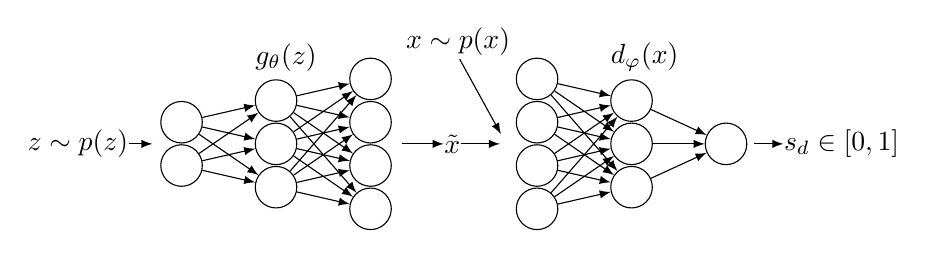
\begin{tikzpicture}
  % code
  \node[const]           (z) {$\vc{z} \sim p(\vc{z})$};
  \node[const, right = 0.3cm of z]           (zin) {};
  % decoder in
  \node[latent, right = 0.4cm of z, yshift = 0.275cm] (G11) {};
  \node[latent, right = 0.4cm of z, yshift = -0.275cm] (G12) {};
  % decoder hidden
  \node[latent, right = 1.6cm of z, yshift = 0.55cm] (G21) {};
  \node[latent, right = 1.6cm of z, yshift = 0cm] (G22) {};
  \node[latent, right = 1.6cm of z, yshift = -0.55cm] (G23) {};
  % decoder out
  \node[latent, right = 2.8cm of z, yshift = 0.825cm] (G31) {};
  \node[latent, right = 2.8cm of z, yshift = 0.275cm] (G32) {};
  \node[latent, right = 2.8cm of z, yshift = -0.275cm] (G33) {};
  \node[latent, right = 2.8cm of z, yshift = -0.825cm] (G34) {};
  % generator tag
  \node[const, right = 1.6cm of z, yshift = 1.1cm] (G) {$g_{\vc{\theta}}(\vc{z})$};
  % x
  \node[const, right = 4.0cm of z]           (xg) {$\tilde{\vc{x}}$};
  \node[const, right = -0.8cm of xg]          (xout) {};
  \node[const, right = 0.5cm of xg]           (xin) {};
  \node[const, right = -0.7cm of xg, yshift=1.3cm]      (x) {$\vc{x} \sim p(\vc{x})$};
  \node[const, right = -0.05cm of xg, yshift=1.1cm]      (xpout) {};
  \node[const, right = 0.5cm of xg, yshift=0.1cm]      (xpin) {};
  % encoder in
  \node[latent, right = 0.7cm of xg, yshift = 0.825cm] (D11) {};
  \node[latent, right = 0.7cm of xg, yshift = 0.275cm] (D12) {};
  \node[latent, right = 0.7cm of xg, yshift = -0.275cm] (D13) {};
  \node[latent, right = 0.7cm of xg, yshift = -0.825cm] (D14) {};
  % encoder hidden
  \node[latent, right = 1.9cm of xg, yshift = 0.55cm] (D21) {};
  \node[latent, right = 1.9cm of xg, yshift = 0cm] (D22) {};
  \node[latent, right = 1.9cm of xg, yshift = -0.55cm] (D23) {};
  % encoder out
  \node[latent, right = 3.1cm of xg, yshift = 0cm] (D31) {};
  % xhat
  \node[const, right = 4.1cm of xg]           (dx) {$s_d \in [0,1]$};
  \node[const, right = -1.9cm of dx]       (dxout) {};       
  % discriminator tag
  \node[const, right = 1.9cm of xg, yshift = 1.1cm] (D) {$d_{\vc{\varphi}}(\vc{x})$};
  
  % edges
  % latent
  \nedge {z} {zin}
  % generator
  \nedge {G11, G12} {G21, G22, G23}
  \nedge {G21, G22, G23} {G31, G32, G33, G34} 
  
  % x 
  \nedge {xout} {xg}
  \nedge {xg} {xin}
  \nedge {xpout} {xpin}
  % discriminator
  \nedge {D11, D12, D13, D14} {D21, D22, D23}
  \nedge {D21, D22, D23} {D31}
  %xhat
  \nedge {dxout} {dx}
\end{tikzpicture}
\caption{A schematic of a GAN consisting of fully connected layers. A latent
noise sample $\vc{z}\sim p(\vc{z})$ is fed to the generator $g_{\vc{\theta}}(\vc{z})$
which then produces an artificial sample $\tilde{\vc{x}}$. Alternatively,
a sample $\vc{x}$ is sampled from the data distribution $p(\vc{x})$. Both
are passed to the discriminator $d_{\vc{\varphi}}(\vc{x})$ that produces a score
$s_d$ -- the probability that $\tilde{\vc{x}}$ or $\vc{x}$ come from the
true data distribution.}
\label{fig:gan}
\end{figure}

Suppose that we have samples from the true data distribution $p(\vc{x}),\vc{x}\in\mathcal{X}$, which we are trying to imitate. We don't know the true form of $p(\vc{x})$, since it is usually high-dimensional and not representable directly by a function, but instead it is available to us through a finite set of samples that comprise the training dataset $X = \lbrace \vc{x}_1, \vc{x}_2, \ldots, \vc{x}_n \rbrace \subset \mathcal{X}$. The goal is to build a proxy for $p(\vc{x})$ so that we can draw new, yet unseen samples from it. The GAN tackles this problem by a model with two principal parts. First is the \textbf{generator}, which is a neural network that represents a mapping $g_{\vc{\theta}}(\vc{z}):\mathcal{Z}\rightarrow\mathcal{X}$, where $\vc{\theta}$ are its weights, and $\mathcal{Z}$ is the latent space. Note that we use the same notation for the generator that was already used for a decoder in the AE model -- this is because they fulfill the same role in both models. We will denote a generated sample by $\tilde{\vc{x}} = g_{\vc{\theta}}(\vc{z})$. Since the generator as we have defined it so far is deterministic and we need to cover a random distribution, the inputs to the generator come from a \textbf{prior} noise distribution $p(\vc{z})$. The prior is usually chosen such that it it easy to generate samples from it, e.g. $p(\vc{z}) = \mathcal{N}(0,\vc{I})$, in which case $\mathcal{Z} = \mathbb{R}^h$ with $h$ being the dimension of the latent space. Then, the task is to train the generator in such a fashion that it learns the potentially highly non--linear mapping from $p(\vc{z})$ to $p(\vc{x})$. This is stimulated by the adversary of the generator -- the \textbf{discriminator}. We define it as a neural network with weights $\vc{\theta}$, i.e. a mapping $d_{\vc{\varphi}}(\vc{x}):\mathcal{X}\rightarrow\left[0,1\right]$. The output of the discriminator has the interpretation of the probability that its input comes from $p(\vc{x})$ rather than being generated by the generator, in other words, true samples $\vc{x}$ should be given higher value than the generated samples $\tilde{\vc{x}}$.

Both parts of a GAN are trained (their weights are updated) in tandem, so each of them iteratively improves in its task. The discriminator is trained both with true and generated samples to maximize the probability of assigning the correct label to them, while the generator is minimizing the probability of the discriminator recognizing the generated sample. This can be written down as a two player minimax~\cite{maschler2020game} game 
\begin{equation} \label{eq:gan_obj}
\min_{\vc{\theta}}\max_{\vc{\varphi}}\mathbb{E}_{ \vc{x} \sim p(\vc{x})}\left[\ln d_{\vc{\varphi}}(\vc{x})\right]+\mathbb{E}_{\vc{z}\sim p(\vc{z})}\left[\ln\left(1-d_{\vc{\varphi}}(g_{\vc{\theta}}(\vc{z}))\right)\right].
\end{equation}
It can be shown~\cite{goodfellow2014gan} that this objective has a saddle point at at $-\ln4$. In practice, \eqref{eq:gan_obj} is not used directly. That is because the term $\ln\left(1-d_{\vc{\varphi}}(g_{\vc{\theta}}(\vc{z}))\right)$ suffers from vanishing gradients -- when the generated samples do not resemble the real data in the beginning of the training, than this terms is almost zero and the generator is not trained. Therefore, instead of minimizing this, we can maximize $\ln d_{\vc{\varphi}}(g_{\vc{\theta}}(\vc{z}))$ to train the generator, which has much stronger gradients~\cite{goodfellow2014gan}. During training, we sample $\vc{x}$ from the training dataset and $\vc{z}$ from the prior distribution and update the generator and discriminator weights by minimizing
\begin{equation}\label{eq:gen_loss}
\mathcal{L}_{g}(\vc{z},\vc{\theta})= - \ln d_{\vc{\varphi}}(g_{\vc{\theta}}(\vc{z})),
\end{equation}
\begin{equation}\label{eq:disc_loss}
\mathcal{L}_{d}(\vc{x},\vc{z},\vc{\varphi})= - \ln d_{\vc{\varphi}}(\vc{x}) - \ln\left(1-d_{\vc{\varphi}}(g_{\vc{\theta}}(\vc{z}))\right).
\end{equation}
Note that we explicitly remove the dependency of the loss functions on the weights that are not being optimized through them. A detailed training procedure of a GAN is described in Alg.~\ref{alg:gan_train}. Interestingly, during training, the generator never encounters any sample coming from $p(x)$ but is still able to eventually learn the shape of $p(\vc{x})$. The choice of $p(\vc{z})$ can be rather arbitrary as far as sampling from it is possible and the generator and discriminator have sufficient capacity to process it. In practice, uniform or normal distribution is usually used, as already mentioned. 

\begin{algorithm}
\begin{algorithmic}[1]
\Require{Generator $g_{\vc{\theta}}$, discriminator $e_{\vc{\phi}}$, a training set $X=\lbrace \vc{x}_1, \vc{x}_2, \ldots, \vc{x}_n \rbrace \subset \mathcal{X}$, maximum number of iterations $I\in\mathbb{N}$, batchsize $L \in \mathbb{N}$.}
\State $\vc{\theta}, \vc{\varphi} \gets $ Initialize weights
\State{$i \gets $ Iteration counter}
\While{$i<I$ or $\vc{\theta}, \vc{\varphi}$ are not converged}
	\State{$X_L \gets$ A random batch of $L$ samples from $X$}
	\State{$Z_L \gets$ A random batch of $L$ samples from $p(\vc{z})$}
	\State$l_d \gets \frac{1}{L}\sum_{j=1}^L \mathcal{L}_d(\vc{x}_j,\vc{z}_j,\vc{\varphi}), \vc{x}_j \in X_L, \vc{z}_j \in Z_L$
	\State$\vc{\varphi} \stackrel{+}\gets - \nabla_{\vc{\varphi}} l_d$ update of discriminator weights 
	\State$l_g \gets \frac{1}{L}\sum_{j=1}^L \mathcal{L}_g (\vc{z}_j,\vc{\theta}), \vc{z}_j \in Z_L$
	\State$\vc{\theta} \stackrel{+}\gets - \nabla_{\vc{\theta}} l_g$ update of generator weights
	\State{$i \gets i+1$}
\EndWhile
\State{\textbf{return} generator $g_{\vc{\theta}}(\vc{z})$, discriminator $d_{\vc{\varphi}}(\vc{x})$}
\end{algorithmic}
\caption{GAN training procedure.}
\label{alg:gan_train}
\end{algorithm}

Achieving convergence such that the generated samples $\tilde{\vc{x}}$ resemble the training data might be difficult and require multiple random initializations of the model weights. Details on stable training of GANs can be found e.g. in~\cite{gui2021review}. A phenomenon called \textbf{mode collapse} has been described~\cite{goodfellow2016nips}, which happens when $p(\vc{x})$ is multimodal, but the generator distribution collapses to a single mode. A generator that has collapsed to a single mode of a MNIST dataset will produce only a single digit, e.g. "1", no matter where the code is sampled from. To mitigate this issue, several practices have been proposed~\cite{salimans2016fmgan,hong2019generative}. One of them is the use of an enhanced generator loss
\begin{equation} \label{eq:fmgan}
\mathcal{L}_{\text{gfm}}(\vc{z},\vc{x},\vc{\theta})=\alpha\mathcal{L}_{g}(\vc{z},\vc{\theta})+\mathcal{L}_{h}(\vc{z},\vc{x},\vc{\theta}),
\end{equation}
where the second term is the so-called \textbf{feature-matching} loss
\begin{equation} \label{eq:fm_loss}
\mathcal{L}_{fm}(\vc{z},\vc{x},\vc{\theta}) = ||d_{l,\vc{\varphi}}(\vc{x})-d_{l,\vc{\varphi}}(g_{\vc{\theta}}(\vc{z}))||_{2}^{2}
\end{equation}
where $\alpha > 0$ is a tunable weight and $d_{l,\vc{\varphi}}(\vc{x})$ is the intermediate representation of $\vc{x}$ after propagation through $l \in \mathbb{N}$ layers of the discriminator. This loss is supposed to provide improved gradients for the generator to stabilize the training. In the following text, a GAN model with the loss~(\ref{eq:fmgan}) will be referred to as the \textbf{feature-matching GAN} (fmGAN).

\subsection{GANs in anomaly detection}
The idea of using a GAN for anomaly detection comes from the the ability of the generator to learn the true data distribution $p(\vc{x})$ and especially the ability of the discriminator to recognize samples coming from $p(\vc{x})$. When the training dataset consists of normal samples, the discriminator output can be converted into an anomaly score
\begin{equation} \label{eq:disc_score}
     s_{\text{GAN}}(\vc{x}) = 1 - d_{\vc{\varphi}}(\vc{x}),
\end{equation}
which is higher for suspected anomalies and lower for normal data. The common critique is that the discriminator was not trained to recognize an arbitrary distribution of the anomalies but only that of the latent transformed by the generator. Thus it may fail to recognize anomalous samples of interest. 

The authors of the \textbf{AnoGAN} model~\cite{schlegl2017unsupervised} recognize this flaw. Their convolutional GAN model is trained with the feature-matching loss~\eqref{eq:fmgan}. For identification of anomalies in medical images, instead of using~\eqref{eq:disc_score}, they propose an iterative procedure that searches for the latent code $\vc{z}$ most likely to generate the tested sample to identify anomalous images. However, this procedure is computationally expensive. Therefore, an update to this model was published, the \textbf{f(ast)AnoGAN}~\cite{schleglFAnoGANFastUnsupervised2019}. It uses a Wasserstein GAN~\cite{gulrajani2017improved,haloui2018anomaly} (more on Wasserstein optimization objective in the next section) with gradient penalization~\cite{gulrajani2017improved} to improve training stability and adds an encoder distribution $q_{\phi}(\vc{z}|\vc{x})$ to find $\vc{z}$ closest to given $\vc{x}$ faster. The anomaly score of fAnoGAN is a combination of the discriminator score~\eqref{eq:disc_score} and the feature-matching loss~\eqref{eq:fm_loss}. 

The fmGAN model is used the publication~\cite{kliger2018novelty}, where it is tested on benchmark datasets such as MNIST and CIFAR-10. In~\cite{wang2018generative}, a GAN model was used to detect anomalies in time series data coming from industrial processes, whereas in~\cite{zenatiEfficientGANBasedAnomaly2018}, network intrusions were detected. In the \textbf{Multiple-Objective Generative Adversarial Active Learning} (MOGAAL)~\cite{liu2019generative}, $k \in \mathbb{N}$ generators are trained against a single discriminator on input data divided into $k$ subsets. The discriminator score Eq.~\eqref{eq:disc_score} is used to test new samples. The authors of~\cite{perera2019ocgan} claim to have achieved state-of-the-art results in one-class classification through severely restricting the latent space of the
GAN combined with an autoencoder and employing an adversarial data augmentation strategy. 

The use of GAN with an encoder~\cite{donahue2016adversarial} or an autoencoder with a discriminator~\cite{leveau2017adversarial} for anomaly detection is often and somehow blurs the line between GAN and VAE-based models, but we believe that presenting both concepts separately is useful. True GAN-like models for anomaly detection are however far less prevalent than models that use some autoencoding structure, which will be the focus of the next section. Experimental comparison of both approaches is presented in Chapter~\ref{sec:chapter_comparison}.

\section{VAE-based models} \label{sec:vae_models}
The \textbf{Variational Autoencoder} (VAE) is a generative model that has enjoyed a great success in a number of fields since its introduction in~\cite{kingma2013vae}. Its basic architecture~\cite{kingma2019introduction} is very similar to that of an AE model described in Sec.~\ref{sec:reconstruction_models}, but that is where the similarities end, as VAE is more of a probabilistic anomaly detector, since it models the probability distribution of the normal data. Unlike in AE, where the encoding to latent space $\mathcal{Z}$ is not constrained from taking any shape or form as far as the learning objective is minimized, in VAE a desired distribution of the encodings is explicitly prescribed in the form of a prior distribution $p(\vc{z})$. If the network is trained properly and the encodings follow the prior, we can feed samples from $p(\vc{z})$ to the decoder and expect to obtain random samples in the $\mathcal{X}$ space that will resemble those from the training dataset. This is the simple principle of how VAE works --- more details will be given in the following text.

The VAE has been mainly used for generation of artificial images such as faces~\cite{rezende2014stochastic} or sentences~\cite{bowman2015generating}, but also for other tasks such as semi--supervised learning~\cite{kingma2014semi}, segmentation~\cite{sohn2015learning}, static image forecasting~\cite{walker2016uncertain} and of course for anomaly detection~\cite{an2015variational,xu2018unsupervised,solch2016variational}. Since its popularity, a multitude of approaches enhancing the original VAE has been published, approaching the paradigm from different angles, with some of the more prominent examples published in~\cite{higgins2017beta,zhao2017infovae,tolstikhin2017wasserstein,makhzani2015adversarial,pu2017adversarial}. In the following text, we will go through the basic theory, its implications for the basic VAE, and through some of the extensions. 

\subsection{Basic VAE} \label{sec:vanilla_vae}
We will begin by defining the VAE from a probabilistic perspective. Let us assume that there is a dataset $X$ consisting of i.i.d samples. We want to obtain a tractable estimate of the true data distribution $p(\vc{x})$ in order to be able to sample from it. For that purpose, suppose that there is a hidden random process that generates the data and which involves a latent variable $\vc{z}$. Then, like in the case of the GAN model, we can redirect the sampling from the data space $\mathcal{X}$ to the latent space
$\mathcal{Z}$, in which it might be easier. Specifically, we want to sample from the latent prior distribution specified by a density $p(\vc{z})$, then pass this sample to the generative distribution with density $p_{\vc{\theta}}(\vc{x}|\vc{z})$, where $\vc{\theta}$ are its parameters, and obtain a sample $\vc{x}$ that will be very similar to the samples coming from the true data distribution $p(\vc{x})$. In other words, we want to maximize the probability of each sample obtained through the generative process
\begin{equation}
p_{\vc{\theta}}(\vc{x})=\int_{\mathcal{Z}}p_{\vc{\theta}}(\vc{x}|\vc{z})p(\vc{z})d\vc{z}.\label{eq:x_likelihood}
\end{equation}
Unfortunately, there are several issues with this. Firstly, we do not know the optimal value of parameters $\vc{\theta}$. Secondly, the integral~(\ref{eq:x_likelihood}) is usually intractable, e.g. in the case where $p_{\vc{\theta}}(\vc{x}|\vc{z})$ is represented by a neural network. Finally, we want to avoid expensive sampling methods such as Monte Carlo Expectation Maximization~\cite{levine2001implementations}. A sampling procedure is eventually used, but we only want to pass such samples $\vc{z}$ to the generative model that will already be very likely under $p_{\vc{\theta}}(\vc{x}|\vc{z})$. To this end, we introduce a discriminative distribution $q_{\vc{\phi}}(\vc{z}|\vc{x})$ which is an approximation of the true intractable posterior $p(\vc{z}|\vc{x})$, with parameters $\vc{\phi}$.

\subsubsection{The ELBO objective}
Now, we would like to relate the generative and discriminative distributions together in way that would enable us to optimize the model with respect to $\vc{\phi},\vc{\theta}$. Continuing from~(\ref{eq:x_likelihood}),
\begin{equation}
\ln p_{\vc{\theta}}(\vc{x})=\mathbb{E}_{q_{\vc{\phi}}(\vc{z}|\vc{x})}\left[\ln p_{\vc{\theta}}(\vc{x})\right]=\mathbb{E}_{q_{\vc{\phi}}(\vc{z}|\vc{x})}\left[\ln p_{\vc{\theta}}(\vc{x}|\vc{z})+\ln p(\vc{z})-\ln p(\vc{z}|\vc{x})\right],
\end{equation}
where we have used the Bayes' rule and the fact that $p_{\vc{\theta}}(\vc{x})$ does not depend on $\vc{z}$. Now we use the KL divergence~\eqref{eq:kld}
\begin{eqnarray}
\ln p_{\vc{\vc{\theta}}}(\vc{x})-D_{\text{KL}}\left(q_{\vc{\phi}}(\vc{z}|\vc{x})||p(\vc{z}|\vc{x})\right) & = & \mathbb{E}_{q_{\vc{\phi}}(\vc{z}|\vc{x})}\left[\ln p_{\vc{\theta}}(\vc{x}|\vc{z})+\ln p(\vc{z})-\ln q_{\vc{\phi}}(\vc{z}|\vc{x})\right]\label{eq:elbo1}\\
 & = & \mathbb{E}_{q_{\vc{\phi}}(\vc{z}|\vc{x})}\left[\ln p_{\vc{\theta}}(\vc{x}|\vc{z})\right]-D_{\text{KL}}\left(q_{\vc{\phi}}(\vc{z}|\vc{x})||p(\vc{z})\right)\label{eq:elbo2}\\
 & = & - \mathcal{L}_{\text{VAE}}(\vc{x},\vc{\phi},\vc{\theta})\label{eq:elbo3}
\end{eqnarray}
This is the variational lower bound of the VAE model, sometimes called \textbf{ELBO} (evidence lower boundary) through which we can optimize the marginal likelihood $p_{\vc{\theta}}(\vc{x})$. This is due to the fact that the analytically unsolvable term $D_{\text{KL}}\left(q_{\vc{\phi}}(\vc{z}|\vc{x})||p(\vc{z}|x)\right)$ is always nonnegative, thus by maximization of ELBO (minimization of $\mathcal{L}_{\text{VAE}}(\vc{x},\vc{\phi},\vc{\theta})$) we also maximize $p_{\vc{\theta}}(\vc{x})$.

By looking at the individual parts of Eq.~(\ref{eq:elbo2}), we can see that by maximizing the ELBO, we simultaneously maximize the likelihood $p_{\vc{\theta}}(\vc{x}|\vc{z})$ and minimize the distance between $q_{\vc{\phi}}(\vc{z}|\vc{x})$ and $p(\vc{z})$. While looking at the left--hand side of \eqref{eq:elbo1} we can see that at the same time, the marginal likelihood $p_{\vc{\theta}}(\vc{x})$ is maximized and the error term $D_{\text{KL}}\left(q_{\vc{\phi}}(\vc{z}|\vc{x})||p(\vc{z}|\vc{x})\right)$ is minimized, forcing the shape of $q_{\vc{\phi}}(\vc{z}|\vc{x})$ to the true posterior. Also, \eqref{eq:elbo2} captures the autoencoding nature of the VAE model. We pass $\vc{x}$ to the discriminative distribution, which acts as an encoder, sample latent encoding $\vc{z} \sim q_{\vc{\phi}}(\vc{z}|\vc{x})$ and pass this back to generative distribution, which acts as a decoder, to obtain a reconstructed sample $\vc{x}' \sim p_{\vc{\theta}}(\vc{x}|\vc{z})$. From this point on, we will use the term encoder and decoder to describe the discriminative and generative distributions.

\begin{figure}
\centering{}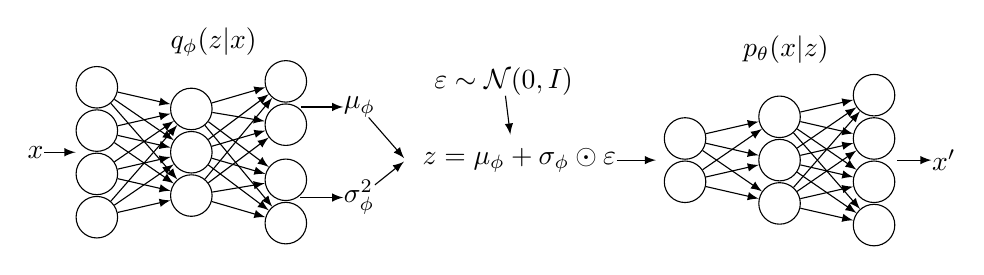
\begin{tikzpicture}
  \node[const]                               (x) {$\vc{x}$};
  \node[const, right = 0.4cm of x]           (xin) {};
  % encoder in
  \node[latent, right = 0.4cm of x, yshift = 0.825cm] (E11) {};
  \node[latent, right = 0.4cm of x, yshift = 0.275cm] (E12) {};
  \node[latent, right = 0.4cm of x, yshift = -0.275cm] (E13) {};
  \node[latent, right = 0.4cm of x, yshift = -0.825cm] (E14) {};
  % encoder hidden
  \node[latent, right = 1.6cm of x, yshift = 0.55cm] (E21) {};
  \node[latent, right = 1.6cm of x, yshift = 0cm] (E22) {};
  \node[latent, right = 1.6cm of x, yshift = -0.55cm] (E23) {};
  % encoder out
  \node[latent, right = 2.8cm of x, yshift = 0.9cm] (E31) {};
  \node[latent, right = 2.8cm of x, yshift = 0.35cm] (E32) {};
  \node[latent, right = 2.8cm of x, yshift = -0.35cm] (E33) {};
  \node[latent, right = 2.8cm of x, yshift = -0.9cm] (E34) {};
  % encoder tag
  \node[const, right = 1.6cm of x, yshift = 1.4cm] (ED) {$q_{\vc{\phi}}(\vc{z}|\vc{x})$};
  % code
  \node[const, right = 3.8cm of x, yshift = 0.575cm]           (mu) {$\vc{\mu}_{\vc{\phi}}$};
  \node[const, right = 3.8cm of x, yshift = -0.575cm]           (sigma) {$\vc{\sigma}^2_{\vc{\phi}}$};
  \node[const, right = -1.0cm of mu]           (muout) {};       
  \node[const, right = -1.0cm of sigma]           (sigmaout) {};       
  \node[const, right = 4.8cm of x, yshift=-0.1cm]           (z) {$z=\mu_{\vc{\phi}}+\sigma_{\vc{\phi}} \odot \varepsilon$};
  \node[const, right = -2.7cm of z]           (zout) {};
  \node[const, right = 4.95cm of x, yshift = 0.9cm]         (epsilon) {$\varepsilon \sim \mathcal{N}(0,\vc{I})$};
  \node[const, right = 5.9cm of x, yshift = 0.2cm]         (epsilonin) {};
  \node[const, right = 0.5cm of z]           (zin) {};
  % decoder in
  \node[latent, right = 0.6cm of z, yshift = 0.275cm] (D11) {};
  \node[latent, right = 0.6cm of z, yshift = -0.275cm] (D12) {};
  % decoder hidden
  \node[latent, right = 1.8cm of z, yshift = 0.55cm] (D21) {};
  \node[latent, right = 1.8cm of z, yshift = 0cm] (D22) {};
  \node[latent, right = 1.8cm of z, yshift = -0.55cm] (D23) {};
  % decoder out
  \node[latent, right = 3cm of z, yshift = 0.825cm] (D31) {};
  \node[latent, right = 3cm of z, yshift = 0.275cm] (D32) {};
  \node[latent, right = 3cm of z, yshift = -0.275cm] (D33) {};
  \node[latent, right = 3cm of z, yshift = -0.825cm] (D34) {};
  % xhat
  \node[const, right = 4cm of z]           (xhat) {$\vc{x}'$};
  \node[const, right = -0.8cm of xhat]       (xhatout) {};    
  % decoder tag
  \node[const, right = 1.6cm of z, yshift = 1.4cm] (DD) {$p_{\vc{\theta}}(\vc{x}|\vc{z})$};   
  
  % edges
  \nedge {x} {xin}
  % encoder 
  \nedge {E11, E12, E13, E14} {E21, E22, E23}
  \nedge {E21, E22, E23} {E31, E32, E33, E34}
  % latent
  \nedge {muout} {mu}
  \nedge {sigmaout} {sigma}
  \nedge {mu,sigma} {zout}
  \nedge {z} {zin}
  \nedge {epsilon} {epsilonin}
  % decoder
  \nedge {D11, D12} {D21, D22, D23}
  \nedge {D21, D22, D23} {D31, D32, D33, D34} 
  %xhat
  \nedge {xhatout} {xhat}
\end{tikzpicture}

\caption{A schematic of a Variational Autoencoder consisting of fully connected layers with a Gaussian encoder $q_{\vc{\phi}}(\vc{z}|\vc{x})$ with mean $\vc{\mu}_{\vc{\phi}}$ and variance $\vc{\sigma}^2_{\vc{\phi}}$, which are extracted from the last layer of the encoder. They are used to sample an encoding $\vc{z}$ through the reparametrization trick with a noise variable $\varepsilon$. The encoding is then passed forward and the reconstruction $\vc{x}'$ is sampled from the decoder $p_{\vc{\theta}}(\vc{x}|\vc{z})$.}
\label{fig:vae}
\end{figure}

\subsubsection{Vanilla VAE}
To be able to optimize~\eqref{eq:elbo3}, we must make some additional assumptions about the model. Here, we will describe those that were made by the authors of the original "vanilla" VAE model, but note that different choices are also possible. First, the \textbf{prior} $p(\vc{z})$ is chosen to be an $h$-dimensional unit normal distribution $p(\vc{z})=\mathcal{N}(\vc{z}|0,\textbf{I})$. The encoded training data are expected to follow this distribution after optimization and it is used for generation of new samples. In tandem with this, the encoder is assumed to model a normal distribution with diagonal covariance matrix $q_{\vc{\phi}}(\vc{z}|\vc{x})=\mathcal{N}\left(\vc{z}|\mu_{\vc{\phi}}(x), \text{diag}(\vc{\sigma}^2_{\vc{\phi}}(x))\right), \vc{\mu}_{\vc{\phi}}, \vc{\sigma}^2_{\vc{\phi}}:\mathbb{R}^d \rightarrow \mathbb{R}^h$, where the mean and variance estimates are computed by neural networks with shared weights $\vc{\phi}$. These choices lead to an analytically solvable expression for the KL divergence in~\eqref{eq:elbo2}, see~\eqref{eq:kl_standard} in the Appendix
\begin{equation} \label{eq:vae_kld}
D_{\text{KL}}\left(q_{\vc{\phi}}(\vc{z}|\vc{x})||p(\vc{z}) \right) = \frac{1}{2}\sum_{i=1}^{d} 1-\sigma_{\vc{\phi},i}^{2}(\vc{x})+\ln \sigma_{\vc{\phi},i}^{2}(\vc{x}) -\mu_{\vc{\phi},i}^{2}(\vc{x}).
\end{equation}

Second, the optimization of the ELBO~\eqref{eq:elbo3} requires sampling from the encoder $q_{\vc{\phi}}(\vc{z}|\vc{x})$. This is however problematic for optimization by backpropagation, because sampling is not a differentiable operation. Therefore, a \textbf{reparametrization trick} was introduced in~\cite{kingma2013vae}. Instead of directly drawing samples $z \sim q_{\vc{\phi}}(\vc{z}|\vc{x})$, we first take a sample from an $h$-dimensional noise distribution $\varepsilon\sim p(\varepsilon)=\mathcal{N}(0,\mathbf{I})$ and then compute the encoding as $\vc{z}=\vc{\mu}_{\vc{\phi}}(\vc{x})+\vc{\sigma}^2_{\vc{\phi}}(\vc{x}) \odot \varepsilon$, where $\odot$ denotes element-wise multiplication. This changes the first term of the ELBO, which is called the \textbf{log-likelihood} to
\begin{equation} \label{eq:vae_reparam}
\mathbb{E}_{q_{\vc{\phi}}(\vc{z}|\vc{x})}\left[\ln p_{\vc{\theta}}(\vc{x}|\vc{z})\right] = \mathbb{E}_{\varepsilon\sim\mathcal{N}(0,\textbf{I})}\left[\ln p_{\vc{\theta}}(\vc{x}| \vc{\mu}_{\vc{\phi}}(\vc{x})+\vc{\sigma}^2_{\vc{\phi}}(\vc{x}) \odot \varepsilon )\right].
\end{equation}

Finally, the decoder $p_{\vc{\theta}}(\vc{x}|\vc{z})$ is also assumed to model a normal distribution\\ $\mathcal{N}(\vc{x}|\vc{\mu}_{\vc{\theta}}(\vc{z}),\sigma I), \vc{\mu}_{\vc{\theta}} :\mathbb{R}^h \rightarrow \mathbb{R}^d, \sigma\in\mathbb{R}$, although a Bernoulli distribution is sometimes used for data scaled to the interval [0,1]. The mean of the decoder distribution is again represented by a neural network with weights $\vc{\theta}$. The scalar parameter $\sigma$ is either fixed, or it can be estimated from data during training. Therefore, the log-likelihood takes on the form 
\begin{equation} \label{eq:vae_logpx}
\ln p_{\vc{\theta}}(\vc{x}|\vc{z}) = - \frac{\sigma}{2} \vert \vert \vc{x} - \vc{\mu}_{\vc{\theta}}(\vc{z}) \vert \vert_2^2 - \frac{d}{2} \ln 2\pi - \frac{d}{2} \ln \sigma. 
\end{equation}
Note that the last two terms can be left out of the optimization, since they are not dependent on any inputs or weights. Again, we see the connection with an autoencoding model, where the log-likelihood~\eqref{eq:vae_logpx} has very similar form to the objective~\eqref{eq:ae_objective}. Here, the reconstruction takes the form of $\vc{x}' = \vc{\mu}_{\vc{\theta}}(\vc{z})$. A notable property of the VAE model is that the reconstruction is stochastic, which is due to the sampling used in the reparametrization trick~\eqref{eq:vae_reparam}. 

Now, we combine the assumptions and equations~\eqref{eq:vae_kld}--\eqref{eq:vae_logpx} to derive the final analytic form of the ELBO objective. The expectation in~\eqref{eq:vae_reparam} is replaced by a mean of $L$ sample of $z$ through the reparametrization trick. The VAE loss function, that is minimized with respect to $\vc{\phi}, \vc{\theta}$, and which is in fact equal to negative ELBO~\eqref{eq:elbo3}, has the form
\begin{equation} \label{eq:vae_loss}
\mathcal{L_{\text{VAE}}}(\vc{x},\vc{\phi},\vc{\theta})=\frac{1}{\sigma L}\sum_{l=1}^{L}||\vc{x}-\vc{\mu}_{\vc{\theta}}(\vc{z}^{l})||_{2}^{2} - \frac{1}{2}\sum_{i=1}^{d} 1-\sigma_{\vc{\phi},i}^{2}(x)+\ln\sigma_{\vc{\phi},i}^{2}(x)-\mu_{\vc{\phi},i}^{2}(x),
\end{equation}
\begin{equation} 
\vc{z}^l=\vc{\mu}_{\vc{\phi}}(\vc{x})+\vc{\sigma}^2_{\vc{\phi}}(\vc{x}) \odot \varepsilon^l, \varepsilon^l \sim  \mathcal{N}(0,\mathbf{I}). \nonumber
\end{equation}
This can be directly optimized via gradient descent techniques. We set $L=1$ in accordance with~\cite{kingma2013vae}. See Fig.~\ref{fig:vae} for a schematic example of a VAE model. The training procedure of a VAE is described in Alg.~\ref{alg:vae_train}. An example of the outputs of a VAE model trained on the MNIST hand--written digits dataset~\cite{lecun-mnisthandwrittendigit-2010} is in Fig.~\ref{fig:mnist_reconstruction}.

\begin{algorithm}
\begin{algorithmic}[1]
\Require{A VAE model with encoder $q_{\vc{\phi}}(\vc{z}|\vc{x})$ and decoder $p_{\vc{\theta}}(\vc{x}|\vc{z})$, training set $X=\lbrace \vc{x}_1, \vc{x}_2, \ldots, \vc{x}_n \rbrace \subset \mathcal{X}$, maximum number of iterations $I\in\mathbb{N}$, batchsize $B \in \mathbb{N}$.}
\State $\vc{\phi},\vc{\theta} \gets $ Initialize parameters
\State{$i \gets $ Iteration counter}
\While{$i<I$ or $\vc{\phi},\vc{\theta}$ are not converged}
	\State{$X_B \gets$ A random batch of $B$ samples from $X$}
	\State$l \gets \frac{1}{B}\sum_{j=1}^L \mathcal{L}_\text{VAE}(\vc{x}_j,\vc{\phi},\vc{\theta}), \vc{x}_j \in X_B$
	\State$\vc{\phi} \stackrel{+}\gets - \nabla_{\vc{\phi}}l $ update of encoder weights
	\State$\vc{\theta} \stackrel{+}\gets - \nabla_{\vc{\theta}}l $ update of decoder weights
	\State{$i \gets i+1$}
\EndWhile
\State{\textbf{return} encoder $q_{\vc{\phi}}(\vc{z}|\vc{x})$, decoder $p_{\vc{\theta}}(\vc{x}|\vc{z})$}
\end{algorithmic}\caption{Variational Autoencoder training procedure.}
\label{alg:vae_train}
\end{algorithm}

\begin{figure}
\centering{}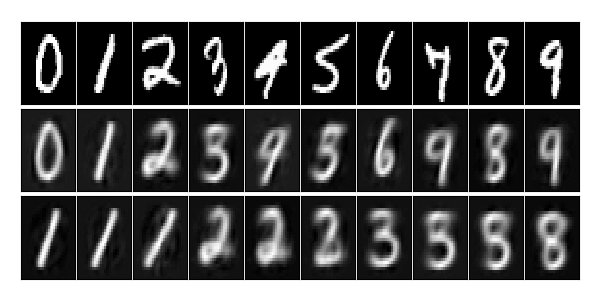
\includegraphics[scale=0.8]{data/chapter_survey/mnist_reconstruction_generation}\caption{Example of a simple VAE trained on the MNIST dataset. Here, the neural networks modelling the encoder and decoder parameters contained two levels of convolutional blocks. Ground truth examples are in the top row, reconstructed samples are in the middle row, artificially generated digits are in the bottom row. The reconstructions are blurry, which is a typical VAE behaviour. Also, the reconstruction is imperfect for digits which resemble each other, such as "9", "4" and "7", or "3" and "8". The artificial digits were created by linearly interpolating between two coordinates in the latent space and using this as an input to the decoder. The VAE then produces a smooth interpolation between digits "1" and "8" that contains the related digits "2" and "3".}
\label{fig:mnist_reconstruction}
\end{figure}
 
\subsubsection{Some VAE properties}
\begin{figure}
\begin{centering}
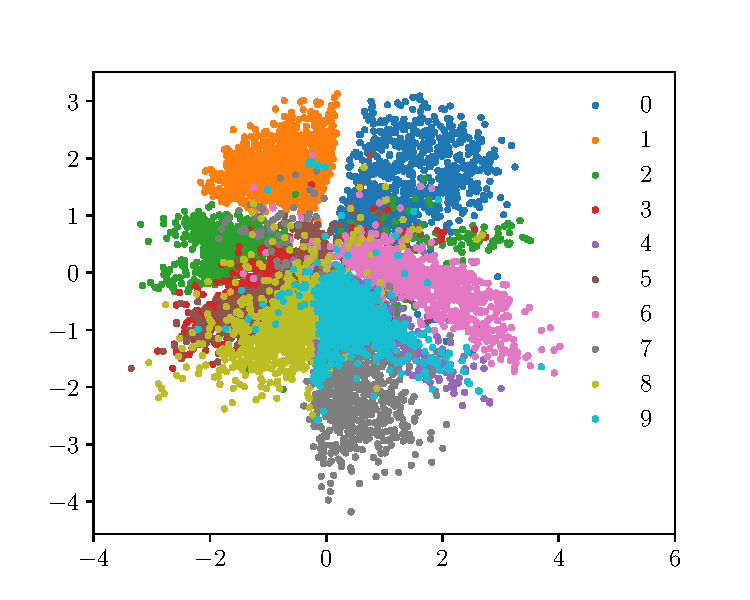
\includegraphics[scale=0.8]{data/chapter_survey/mnist_latent}
\par\end{centering}
\caption{The latent space of the MNIST dataset produced by a VAE with a two-dimensional latent space. Note the overlapping of some digit encodings, e.g. "7" and "9".}
\label{fig:mnist_latent}
\end{figure}

If a VAE model is correctly trained, we can assume that the encoder $q_{\vc{\phi}}(\vc{z}|\vc{x})$ and prior $p(\vc{z})=\mathcal{N}(\vc{z}|0,\textbf{I})$ are close to each other. Then, samples from the prior can be fed to the decoder and one can expect artificial samples that resemble the training data. A \textbf{generated sample} can therefore be described as
\begin{equation} \label{eq:generated_sample}
    \tilde{\vc{x}} = \vc{\mu}_{\vc{\theta}}(\vc{z}), \vc{z} \sim p(\vc{z}).
\end{equation}
Note that a \textbf{reconstructed sample} is instead obtained by sampling the encoding $\vc{z}$ from the encoder through the reparametrization trick~\eqref{eq:vae_reparam}. This is also a place to note why we are using neural network representation of the encoder and decoder. Since neural networks have be proven to be universal function approximators, we know that given enough capacity, data and training time, the decoder can learn a mapping from the prior to an arbitrary function.

\begin{figure}
\centering
    \begin{subfigure}[b]{0.45\textwidth}
        \centering
        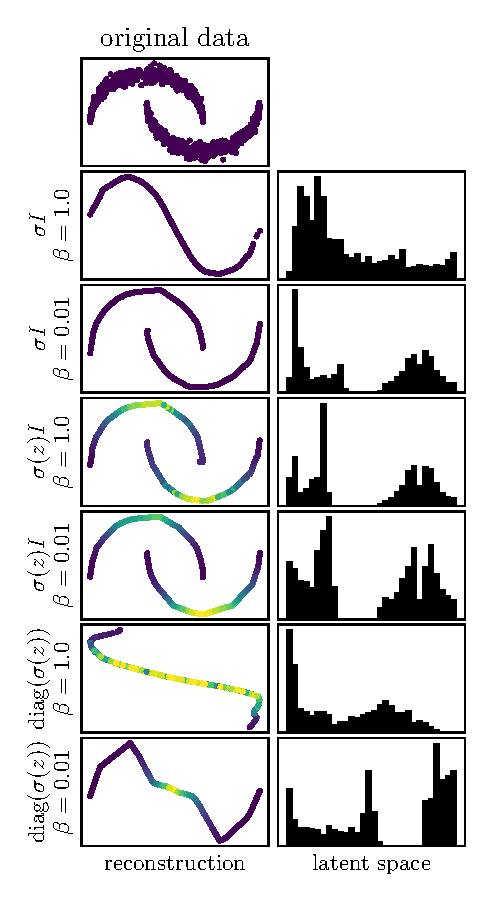
\includegraphics[scale=0.9]{data/chapter_survey/vae_two_moons_z1_colored}
        \caption{$h=1$}
    \end{subfigure}
    \begin{subfigure}[b]{0.45\textwidth}
        \centering
        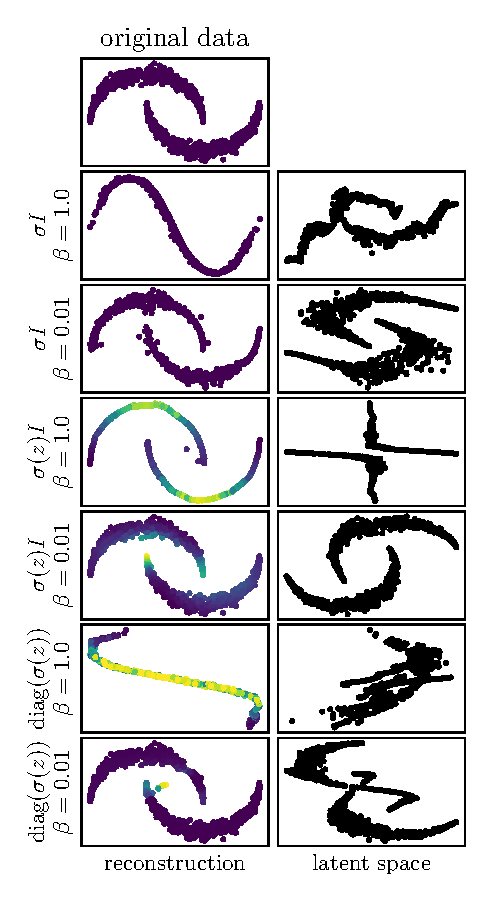
\includegraphics[scale=0.9]{data/chapter_survey/vae_two_moons_z2_colored}
        \caption{$h=2$}
    \end{subfigure}
\caption{An overview of VAE behaviour with respect to the scaling parameter $\beta$ of the objective~\eqref{eq:betavae} and to the way the covariance of the decoder $p_{\vc{\theta}}(\vc{x}|\vc{z})$ is estimated. The VAE model was trained on the two--moons data, plotted in the plots at the very top. Variants with 1D (a) and 2D (b) latent spaces are compared, means of the decoder $\vc{\mu}_{\vc{\theta}}(\vc{z})$ are plotted on the left and the latent representations on the right. Clearly, smaller values of $\beta$ lead to better sample reconstruction, especially in the case of a two-dimensional latent space, as well as leading to a better separation of the encodings. This is understandable, since the prior $p(\vc{z})=\mathcal{N}(0,\textbf{I})$ is unimodal. From the top: the covariance of the decoder is given either by a fixed scalar ($\sigma I,\sigma=1$), by a scalar estimated from the data ($\sigma(\vc{z})I$), or by an estimate of its diagonal terms ($\text{diag}(\sigma(\vc{z}))$). The magnitude of the estimated variance in the two latter cases is denoted by color, where a brighter color corresponds to a higher value of variance. It is interesting that the second case ($\sigma(\vc{z})I$) seems to alleviate the reconstruction difficulties with higher $\beta$, while the estimation of the full covariance diagonal does not exhibit such property. Also, the third case seems to "exploit" the estimation of variance. Instead of pushing and optimizing the mean, it can instead simply put higher variance in the direction in which the reconstruction is worse and still incur only a small loss. Due to this behaviour, the second case seems to be the most robust and stable way of estimation of the reconstruction variance. Not surprisingly, the 2D case provides better reconstructions since it was provided with one more dimension to encode data to.}
\label{fig:betavae}
\end{figure}

Fig.~\ref{fig:mnist_latent} shows the latent space of an example VAE model. Note that although the overall distribution of the encodings resembles the normal prior, in order to be able to reconstruct the samples from the encodings, the model has to learn to encode the samples from different digit classes to different parts of the latent space. It was shown~\cite{higgins2017beta} that the reconstruction and regularization parts of the VAE loss~\eqref{eq:elbo3} actually work against each other. A model with encoder perfectly copying the randomness of the prior would not be able to reconstruct the inputs. On the other hand, a model without the latent regularization would not be able to generate new samples, as it would be practically identical with an AE model from Sec.~\ref{sec:reconstruction_models}, which is free to encode the different classes to arbitrary parts of the latent space. The basic loss~\eqref{eq:vae_loss} leads to a model that is usually in an equilibrium between both of these states. It is however possible to push the model in one of these directions by using a scaling parameter
\begin{equation} \label{eq:betavae}
\mathcal{L}_{\beta\text{VAE}}(\vc{x},\vc{\phi},\vc{\theta},\beta)= - \mathbb{E}_{q_{\vc{\phi}}(\vc{z}|\vc{x})}\left[\ln p_{\vc{\theta}}(\vc{x}|\vc{z})\right] + \beta D_{\text{KL}}\left(q_{\vc{\phi}}(\vc{z}|\vc{x})||p(\vc{z})\right),\beta>0.
\end{equation}
A VAE model trained with this loss is known as \textbf{BetaVAE}~\cite{higgins2017beta} and is one of the first VAE-based models that attempt some sort of \textbf{unsupervised disentanglement}. A disentangled model captures the possible factors of variation of a dataset in orthogonal dimensions of the latent space. Imagine a colored MNIST dataset, on which a disentangled model with a two dimensional latent space is trained. If properly disentangled, one latent dimension would capture the identity of the digit, while the other one would capture its color. This concept will be again revisited in Chapter~\ref{sec:chapter_sgvaegan}. The influence of the $\beta$ parameter is discussed in Fig.~\ref{fig:betavae}.

Instead of setting a fixed variance parameter $\sigma$ in the decoder, one can optimize and extract it instead from the last layer of the decoder, either as a scalar $\sigma_{\vc{\theta}}(\vc{z}) \in \mathbb{R}$
or even a full diagonal of the covariance $\text{diag}\left(\vc{\sigma}_{\vc{\theta}}(\vc{z})\right),\vc{\sigma}(\vc{z})\in\mathbb{R}^{d}$. From the experiment in Fig.~\ref{fig:betavae}, it seems (at least for tabular data) that the best results were surprisingly obtained not by the most complex variant, but the one with a scalar value $\sigma_{\vc{\theta}}$ optimized during training.

\subsection{Wasserstein and adversarial autoencoders}
The asymmetry of the KL divergence motivated search for a more accurate metric measuring the distance between the prior and the encoder. An alternative approach to VAE has been published in~\cite{mescheder2017adversarial} and improved in~\cite{tolstikhin2017wasserstein}, which proposes a general form of a generative autoencoder that uses a Wasserstein metric~\cite{givens1984class}. Unlike the KL divergence term in the VAE loss, which forces all the input data samples to zero (the mean of the standard prior), in \textbf{Wasserstein autoencoders} (WAE) the encoding is loosened, which reportedly leads to improved reconstruction~\cite{tolstikhin2017wasserstein}. A general form of the loss function of a WAE model is
\begin{equation} \label{eq:general_wae_loss}
    \mathcal{L}_{\text{WAE}} (\vc{x}, \vc{\theta}, \vc{\phi}) = - \mathbb{E}_{q_{\vc{\phi}}(\vc{z}|\vc{x})} \left[ \log p_{\vc{\theta}}(\vc{x}|\vc{z}) \right] + \lambda D_{\text{W}} \left( q_{\vc{\phi}}(\vc{z}|\vc{x}) || p(\vc{z}) \right),
\end{equation}
where $\lambda >0$  is a scalar hyperparameter, and $D_{\text{W}}$ is a Wasserstein metric. The most commonly used form of the Wasserstein metric is the kernelized \textbf{maximum-mean-discrepancy} (MMD) with a kernel function $k_f:\mathbb{R}^d \times \mathbb{R}^d \rightarrow \mathbb{R}$, which was reported to perform well in matching high dimensional distributions~\cite{zhao2017infovae}. From the theoretical point of view, KLD only matches the first and the second moment of the two distributions, while MMD can potentially match an infinite amount of moments with the right kernel. Some authors~\cite{tolstikhin2017wasserstein} argue that by minimizing KLD, the latent representation might become uninformative for the decoder to reconstruct the code. On the other hand, MMD maximizes the mutual information between $\vc{x}$  and $\vc{z}$~\cite{zhao2017infovae}.

Under some mild assumptions about the kernel function $k_f$ (see details in~\cite{tolstikhin2017wasserstein}) the MMD can be expressed in such a way that enables optimization of the model by backpropagation. Then, the MMD of the prior and the encoder can be approximated solely by comparing sets of samples from these  distributions $Z_q=\{\vc{z}_{q,1}, \vc{z}_{q,2}, \ldots, \vc{z}_{q,n}\}, Z_p=\{\vc{z}_{p,1}, \vc{y}_{p,2}, \ldots, \vc{y}_{p,n}\},\vc{z}_{q,i}\sim q_{\vc{\phi}}(\vc{z}|\vc{x}),\vc{z}_{p,i} \sim p(\vc{z}),\forall i \in \hat{n}$ in a closed expression
\begin{equation} \label{eq:mmd}
\text{MMD}_{k}(Z_p,Z_q)=\frac{1}{n(n-1)}\sum_{i\neq j}k_f(\vc{z}_{q,i},\vc{z}_{q,j})+\frac{1}{n(n-1)}\sum_{i\neq j}k_f(\vc{z}_{p,i},\vc{z}_{p,j})-\frac{2}{n^{2}}\sum_{i,j}k_f(\vc{z}_{q,i}, \vc{z}_{p,j}).
\end{equation}
The most notable characteristic of the MMD is that in practice, it only require samples from the distributions in question, and it is therefore less restricting than the KLD, which required normal prior and encoder in order to obtain the analytic expression~\eqref{eq:vae_kld}. This offers the potential for the use of a variety of prior and encoder distributions. The two most common choices of $k_f$ are the RBF $k_f(x,y) = \exp(- \gamma \vert \vert x - y \vert \vert_2^2), \gamma > 0$ and inverse multiquadratics (IMQ) $k_f(x,y) = (c^2 +  \vert \vert x - y \vert \vert_2^2)^\beta, c>0, \beta < 0$ kernels. The training algorithm for a Wasserstein autoencoder with the MMD loss is in Alg.~\ref{alg:infovae}. Note that although the parameters $\vc{\phi}$ do not appear directly in the loss on line 7 of the algorithm, they are present through the samples $\tilde{Z_{L}}$. 

\begin{algorithm}
\begin{algorithmic}[1]
\Require{A WAE model with encoder $q_{\vc{\phi}}(\vc{z}|\vc{x})$, decoder $p_{\vc{\theta}}(\vc{x}|\vc{z})$ and a prior $p(\vc{z})$, training set $X=\lbrace \vc{x}_1, \vc{x}_2, \ldots, \vc{x}_n \rbrace \subset \mathcal{X}$, maximum number of iterations $I\in\mathbb{N}$, batchsize $B \in \mathbb{N}$, regularization coefficient $\lambda > 0$, characteristic positive definite kernel $k_f$, standard deviation parameter $\sigma$ > 0.}
\State $\vc{\phi},\vc{\theta} \gets $ Initialize parameters
\State{$i \gets $ Iteration counter}
\While{$i<I$ or $\vc{\phi},\vc{\theta}$ are not converged}
	\State{$X_B \gets$ A random batch of $B$ samples from $X$}
	\State{$Z \gets \lbrace \vc{z}_j \sim q_{\phi}(\vc{z}|\vc{x}_j), \vc{x}_j \in X_B \rbrace$ samples from the encoder}
	\State{$\tilde{Z} \gets$ A random batch of $B$ samples from prior $p(\vc{z})$}
	\State$l \gets \frac{1}{B}\sum_{j=1}^B  ||\vc{x}_j-\vc{\mu}_{\vc{\theta}}(\vc{z}_j)||_{2}^{2} +\lambda \text{MMD}_k(Z,\tilde{Z}), \vc{x}_j \in X_B, \vc{z}_j \in Z$
	\State$\vc{\phi} \stackrel{+}\gets - \nabla_{\vc{\phi}}l $ update of encoder weights
	\State$\vc{\theta} \stackrel{+}\gets - \nabla_{\vc{\theta}}l $ update of decoder weights
	\State{$i \gets i+1$}
\EndWhile
\State{\textbf{return} encoder $q_{\vc{\phi}}(\vc{z}|\vc{x})$, decoder $p_{\vc{\theta}}(\vc{x}|\vc{z})$}
\end{algorithmic}

\caption{InfoVAE training procedure.}
\label{alg:infovae}
\end{algorithm}



\subsection{Adversarial Autoencoder}

A different architecture arises when the Jensen--Shannon divergence
$D_{\text{JS}}$ is used in place of $D_{Z}$. The JS divergence is
a symmetrical (unlike KL divergence) measure of distance between two
probability distributions. The use of $D_{\text{JS}}$ leads to a
model that is called adversarial autoencoder (AAE) and was originally
proposed in~\cite{makhzani2015adversarial}. It was shown in~\cite{tolstikhin2017wasserstein}
how the use of $D_{\text{JS}}$ leads to the use of GAN loss that
was described in the previous part. To regularize the encoder, we
add a discriminator $d_{\eta}(\vc{z}):\mathcal{Z}\rightarrow\left[0,1\right]$
represented by a neural network with parameters $\eta$. The discriminator
has the same function as the one in the GAN model -- it tries to
recognize latent space samples produced by the encoder and those sampled
from the prior $p(\vc{z})$. The difference is that the discriminator now
operates on the latent space $\mathcal{Z}$ instead of the data space
$\mathcal{X}$. 

\begin{figure}
\centering{}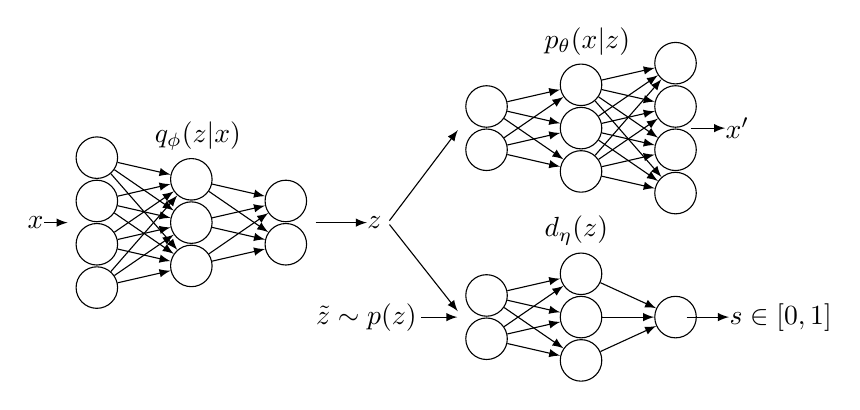
\begin{tikzpicture}
  \node[const]                               (x) {$\vc{x}$};
  \node[const, right = 0.3cm of x]           (xin) {};
  % encoder in
  \node[latent, right = 0.4cm of x, yshift = 0.825cm] (E11) {};
  \node[latent, right = 0.4cm of x, yshift = 0.275cm] (E12) {};
  \node[latent, right = 0.4cm of x, yshift = -0.275cm] (E13) {};
  \node[latent, right = 0.4cm of x, yshift = -0.825cm] (E14) {};
  % encoder hidden
  \node[latent, right = 1.6cm of x, yshift = 0.55cm] (E21) {};
  \node[latent, right = 1.6cm of x, yshift = 0cm] (E22) {};
  \node[latent, right = 1.6cm of x, yshift = -0.55cm] (E23) {};
  % encoder out
  \node[latent, right = 2.8cm of x, yshift = 0.275cm] (E31) {};
  \node[latent, right = 2.8cm of x, yshift = -0.275cm] (E32) {};
  % encoder tag
  \node[const, right = 1.4cm of x, yshift = 1.1cm] (E) {$q_{\vc{\phi}}(\vc{z}|\vc{x})$};
  % placement
  \node[const, right = 5.2cm of x, yshift=1.2cm]           (encoderin) {}; 
  \node[const, right = 5.2cm of x, yshift=-1.2cm]           (discriminatorin) {}; 
  % code
  \node[const, right = 4.1cm of x, yshift = 0cm]           (zg) {$\vc{z}$};
  \node[const, right = 3.4cm of x]           (zgout) {}; 
  \node[const, right = 0cm of encoderin]           (zgin) {};
  \node[const, right = 0.05cm of zg]           (zgout2) {};
  \node[const, right = 0cm of discriminatorin,yshift=0.05cm]           (zgin2) {};
  % prior
  \node[const, right = -1.8cm of discriminatorin, yshift = 0cm]         (z) {$\tilde{\vc{z}} \sim p(\vc{z})$};
  \node[const, right = 0cm of z, yshift = 0cm]         (zout) {};
  \node[const, right = 0cm of discriminatorin]           (zin) {};

  % decoder in
  \node[latent, right = 0.1cm of encoderin, yshift = 0.275cm] (D11) {};
  \node[latent, right = 0.1cm of encoderin, yshift = -0.275cm] (D12) {};
  % decoder hidden
  \node[latent, right = 1.3cm of encoderin, yshift = 0.55cm] (D21) {};
  \node[latent, right = 1.3cm of encoderin, yshift = 0cm] (D22) {};
  \node[latent, right = 1.3cm of encoderin, yshift = -0.55cm] (D23) {};
  % decoder out
  \node[latent, right = 2.5cm of encoderin, yshift = 0.825cm] (D31) {};
  \node[latent, right = 2.5cm of encoderin, yshift = 0.275cm] (D32) {};
  \node[latent, right = 2.5cm of encoderin, yshift = -0.275cm] (D33) {};
  \node[latent, right = 2.5cm of encoderin, yshift = -0.825cm] (D34) {};
  % xhat
  \node[const, right = 3.4cm of encoderin]           (xhat) {$\vc{x}'$};
  \node[const, right = -0.8cm of xhat]       (xhatout) {};    
  % decoder tag
  \node[const, right = 1.1cm of encoderin, yshift = 1.1cm] (D) {$p_{\vc{\theta}}(\vc{x}|\vc{z})$};   
  
  % discriminator
  \node[latent, right = 0.1cm of discriminatorin, yshift = 0.275cm] (DI11) {};
  \node[latent, right = 0.1cm of discriminatorin, yshift = -0.275cm] (DI12) {};
  % discriminator hidden
  \node[latent, right = 1.3cm of discriminatorin, yshift = 0.55cm] (DI21) {};
  \node[latent, right = 1.3cm of discriminatorin, yshift = 0cm] (DI22) {};
  \node[latent, right = 1.3cm of discriminatorin, yshift = -0.55cm] (DI23) {};
  % discriminator out
  \node[latent, right = 2.5cm of discriminatorin, yshift = 0cm] (DI31) {};
  % xhat
  \node[const, right = 3.45cm of discriminatorin]           (dx) {$s \in [0,1]$};
  \node[const, right = -1.9cm of dx]       (dxout) {};       
  % discriminator tag
  \node[const, right = 1.1cm of discriminatorin, yshift = 1.1cm] (D) {$d_{\vc{\eta}}(\vc{z})$};

  % edges
  \nedge {x} {xin}
  % encoder 
  \nedge {E11, E12, E13, E14} {E21, E22, E23}
  \nedge {E21, E22, E23} {E31, E32}
  % latent
  \nedge {zgout} {zg}
  \nedge {zgout2} {zgin}
  \nedge {zgout2} {zgin2}
  \nedge {zout} {zin}

  % decoder
  \nedge {D11, D12} {D21, D22, D23}
  \nedge {D21, D22, D23} {D31, D32, D33, D34} 
  % discriminator
  \nedge {DI11, DI12} {DI21, DI22, DI23}
  \nedge {DI21, DI22, DI23} {DI31}
  %xhat
  \nedge {xhatout} {xhat}
  %xhat
  \nedge {dxout} {dx}

\end{tikzpicture}
\caption{A schematic of a AAE model consisting of fully connected layers. A
data sample $x$ is mapped to latent space representation $\tilde{z}$
via the encoder $q_{\vc{\phi}}(\vc{z}|x)$. Also, a sample $z$ is sampled from
the latent prior $p(\vc{z})$. Both $z$ and $\tilde{z}$ are passed to
the discriminator $d_{\eta}(\vc{z})$ that produces a score $s$ -- the
probability that the input sample comes from the latent prior. At
the same time, the latent representation is passed to the decoder
$p_{\vc{\theta}}(x|z)$ which maps it to a reconstruction $\tilde{x}$.}
\label{fig:aae}
\end{figure}

The GAN loss function~(\ref{eq:disc_loss}) is used to train the
discriminator, while the loss function~(\ref{eq:gen_loss}) is added
to the reconstruction term for training of the encoder and decoder.
The AAE training losses to be maximized are then
\begin{equation}
\mathcal{L}_{d}(\vc{z},\tilde{z},\eta)=\ln d_{\eta}(\vc{z})+\ln(1-d_{\eta}(\tilde{z})),\label{eq:aae_loss_disc}
\end{equation}
\begin{equation}
\mathcal{L}_{ae}(x,\tilde{x},\tilde{z},\vc{\theta},\vc{\phi})=c(x,\tilde{x})-\lambda\ln d_{\eta}(\tilde{z}),\label{eq:aae_loss_autoencoder}
\end{equation}
where $\lambda>0$, $z\sim p(\vc{z})$, $x\sim p(x)$, $\tilde{z}\sim q_{\vc{\phi}}(\vc{z}|x)$
and $\tilde{x}\sim p_{\vc{\theta}}(x|\tilde{z})$.

\begin{algorithm}
\begin{algorithmic}[1]
\Require{An AAE model with encoder $q_{\vc{\phi}}(\vc{z}|\vc{x})$, decoder $p_{\vc{\theta}}(\vc{x}|\vc{z})$,  a prior $p(\vc{z})$ and a discriminator $d_{\vc{\eta}}(\vc{z})$, training set $X=\lbrace \vc{x}_1, \vc{x}_2, \ldots, \vc{x}_n \rbrace \subset \mathcal{X}$, maximum number of iterations $I\in\mathbb{N}$, batchsize $B \in \mathbb{N}$, regularization coefficient $\lambda > 0$, standard deviation parameter $\sigma$ > 0.}
\State $\vc{\phi},\vc{\theta}, \vc{\eta} \gets $ Initialize parameters
\State{$i \gets $ Iteration counter}
\While{$i<I$ or $\vc{\phi},\vc{\theta},\vc{\eta}$ are not converged}
	\State{$X_B \gets$ A random batch of $B$ samples from $X$}
	\State{$Z \gets \lbrace \vc{z}_j \sim q_{\vc{\phi}}(\vc{z}|\vc{x}_j), \vc{x}_j \in X_B \rbrace$ samples from the encoder}
	\State{$\tilde{Z} \gets$ A random batch of $B$ samples from prior $p(\vc{z})$}
	\State{$\tilde{X} \gets \lbrace\tilde{\vc{x}}_j \sim p_{\vc{\theta}}(\vc{x}|\tilde{\vc{z}}_j), \tilde{\vc{z}}_j \in \tilde{Z}_B \rbrace$ generated samples}
	\State$l_{ae} \gets \frac{1}{B}\sum_{j=1}^B \mathcal{L}_{\text{AAE}}( \vc{x}_j,\vc{z}_j,\tilde{\vc{z}}_j, , \vc{\theta}, \vc{\phi} ) , x_j \in X_B, \vc{z}_j \in Z, \tilde{\vc{z}}_j \in \tilde{Z}$
	\State{$l_d \gets \frac{1}{B}\sum_{j=1}^B \mathcal{L}_{\text{AAE}_d}(\vc{z}_j,\tilde{\vc{z}}_j, \vc{\eta}), \vc{z}_j \in Z, \tilde{\vc{z}}_j \in \tilde{Z}$}
	\State$\vc{\phi} \stackrel{+}\gets - \nabla_{\vc{\phi}}l_{ae} $ update of encoder weights
	\State$\vc{\theta} \stackrel{+}\gets - \nabla_{\vc{\theta}}l_{ae} $ update of decoder weights
	\State$\vc{\eta} \stackrel{+}\gets - \nabla_{\vc{\eta}}l_{d} $ update of discriminator weights
	\State{$i \gets i+1$}
\EndWhile
\State{\textbf{return} encoder $q_{\vc{\phi}}(\vc{z}|\vc{x})$, decoder $p_{\vc{\theta}}(\vc{x}|\vc{z})$, discriminator $d_{\vc{\eta}}(\vc{z})$}
\end{algorithmic}

\caption{AAE training procedure.}
\label{alg:aae}
\end{algorithm}

The AAE training procedure is described in Alg.~\ref{alg:aae}.
Again, any prior $p(\vc{z})$ that we can sample from is suitable for the
regularization of AAE, even a multimodal one. A schematic of the AAE
model is in Fig.~\ref{fig:aae}. In practice, an AAE model compared
to InfoVAE behaves similarly as GAN compared to VAE. The adversarial
loss leads to less blurry reconstructions and generated samples at
the cost of higher training instability~\cite{tolstikhin2017wasserstein}.
One way to gain advantages of both is to use an AAE model as depicted
in Fig.~\ref{fig:aae} and add the MMD regularization term~(\ref{eq:mmd})
to the loss~(\ref{eq:aae_loss_autoencoder}).













As was already demonstrated, a common criticism of the VAE model is its use of the unit normal prior $p(\vc{z})$ which stimulates the distribution $q_{\vc{\phi}}(\vc{z}|\vc{x})$ to have a single mode, and therefore it is hard to fit data with a multi-modal latent distribution. The publication~\cite{tomczak2018vae} proposes a learnable multimodal \textbf{Vamp} prior realized as a mixture of $K \in \mathbb{N}$ independent Gaussian components. However, the Vamp prior is not compatible with the basic VAE model since its use does not lead to an analytical expression of KLD~\eqref{eq:vae_kld}. In the following text, we will describe alternatives to KLD regularization that are viable with this kind of prior. Then, the parameters of the components of the mixture are learned together with the parameters of the model.

\subsection{VAE in anomaly detection}
From the anomaly detection perspective, the basic criterion that test whether an input $\vc{x}$ is from the training (normal) data distribution is based on an estimate of the log-likelihood $- \ln p_{\vc{\theta}}(\vc{x}|\vc{z})$ is computed. However, using only the generating model with a prior
\begin{equation}
- \mathbb{E}_{p(\vc{z})}\left[\ln p_{\vc{\theta}}(x|z)\right]
\end{equation}
is theoretically well--justified, but it has been shown that this does not work well enough in practice~\cite{xu2018unsupervised}. Instead, the generative and discriminative distributions are used together to compute an estiamte of the \textbf{sampled reconstruction probability}
\begin{equation} \label{eq:rec_prob}
s_{\text{VAE}}(\vc{x})=-\frac{1}{L}\sum_{l=1}^{L}\ln p_{\vc{\theta}}(\vc{x}|\vc{z}^{l}) \approx-\mathbb{E}_{q_{\vc{\phi}}(\vc{z}|\vc{x})}\left[\ln p_{\vc{\theta}}(\vc{x}|\vc{z})\right].
\end{equation}
\begin{equation}
\vc{z}^l \sim q_{\vc{\phi}}(\vc{z}|\vc{x}) \nonumber 
\end{equation}
which was done in one of the first application of VAE in anomaly detection in~\cite{an2015variational}, where the authors successfully compare the VAE with AE and PCA on several anomaly datasets while claiming that the generative property of VAE can be used for causal analysis on the detected anomalies. Note that for a normal decoder, equation~(\ref{eq:vae_score}) is very similar to the reconstruction error of an  AE model~\eqref{eq:ae_objective}, with the difference that the reconstruction probability is computed from several samples of the encoder.

The reason for using the reconstruction probability of a VAE instead
of a reconstruction error of AE is the improved generalization that
was described in the previous section. It is discussed in~\cite{dai2017hidden}
that a VAE model is equivalent to a non--linear robust PCA model
and is proficient at dismissing sparse outliers. The authors also
make note of the fact that VAE is very efficient in pruning of unnecessary
latent dimensions in case when the real latent structure has lower
dimension than the chosen VAE latent space. However, sometimes~\cite{pereira2018unsupervised}
the reconstruction error of the VAE is used, which is defined as
\begin{equation}
f_{\text{VAEr}}(x)=-\frac{1}{M}\sum_{m=1}^{M}||x-\mathbb{E}\left[p_{\vc{\theta}}(x|z^{m}(\varepsilon)\right]||_{2}^{2},
\end{equation}
where only the mean of the generative distribution is compared to
the original sample $x$.

Another way of using VAE and other autoencoding models for anomaly
detection is to employ their ability to produce a low--dimensional
representation of high--dimensional data that preserves the important
relations between individual datapoints. Then, an anomaly detection
model (be it a generative or a classical one) can be trained on the
data encoded in the latent space. This two stage approach is especially
useful when the problem is in the image domain and some kind of vectorization
has to be used anyway. Also it enables the combination of countless
different approaches. Usage of this technique will be demonstrated
in one of the next chapters. It is also used in~\cite{dai2019diagnosing},
where both stages are a VAE and the second stage has the same input
and latent space dimensionality (therefore it does not compress data
at all). Although this paper does not present an application in anomaly
detection, it shows an improvement in learning of the latent space
prior. 

In~\cite{xu2018unsupervised} the authors present a so-called DonutVAE
with an enhanced loss function to detect anomalies in times series
data. The architecture is similar to that of a vanilla VAE, but the
loss becomes
\begin{equation}
\mathcal{L}_{\text{DVAE}}(x,\vc{\phi},\vc{\theta})=\mathbb{E}_{q_{\vc{\phi}}(\vc{z}|x)}\left[\beta\ln p(\vc{z})-\ln q_{\vc{\phi}}(\vc{z}|x)+\sum_{t=i}^{T}\alpha_{t}\ln p_{\vc{\theta}}(x|z)\right],\label{eq:donutvae}
\end{equation}
where $x=\{x_{t}\}_{t=1}^{T}$ is a sliding window of the last $T$
observations. Also, $\alpha_{t}=0$ if $x_{t}$ is anomalous or missing
and $\alpha_{t}=1$ otherwise and $\beta=\sum_{t=1}^{T}\alpha_{t}/T$.
The authors then show that usage of this loss function improves overall
results. This however has a caveat -- known anomalous samples must
be available, otherwise the loss~(\ref{eq:donutvae}) is the same
as~(\ref{eq:elbo2}). Furthermore, the authors claim that using
reconstruction probability~(\ref{eq:vae_score}) can be seen as
a weighted kernel density estimate.

The authors of~\cite{zong2018deep} couple an ordinary autoencoder
with a Gaussian mixture model (GMM) represented by a neural network.
The AE reduces the problem dimension to help overcome the curse of
dimensionality, while the GMM model serves as a density estimate in
the latent space. The novelty of the method is in two facts. Firstly,
instead of training parameters of both models separately, they are
learnt jointly which improves the performance of the model. Secondly,
the input of the GMM model is not only the latent representation,
but also the reconstruction error of the sample. The loss is 
\begin{eqnarray}
\mathcal{L}_{\text{DAGMM}}(x,\vc{\phi},\vc{\theta},\omega) & = & ||x-d_{\vc{\theta}}(e_{\vc{\phi}}(x))||_{2}^{2}+\lambda_{1}E_{\omega}(\vc{z})+\lambda_{2}P(\hat{\Sigma)}\\
z & = & \left[e_{\vc{\phi}}(x),||x-d_{\vc{\theta}}(\vc{z})||_{2}^{2}\right]^{T}\\
E_{\omega}(\vc{z}) & = & -\ln\left(\sum_{i=1}^{d}\pi_{\omega,i}\frac{\exp\left(-\frac{1}{2}(\vc{z}-\mu_{\omega,i})^{T}\Sigma_{i}^{-1}(\vc{z}-\mu_{\omega,i})\right)}{\sqrt{|2\pi\Sigma_{\omega,i}|}}\right)
\end{eqnarray}
where we recognize the reconstruction error of the AE, the energy
term $E_{\omega}(\vc{z})$ of the GMM model and a penalization $P(\Sigma)$
that prevents the covariance matrices in the GMM model to become singular,
$\lambda_{1},\lambda_{2}>0$ are scaling parameters. Parameters $\left\{ \pi_{\omega,i},\mu_{\omega,i},\Sigma_{\omega,i}\right\} _{i=1}^{d}$
are the parameters of the GMM model estimated by a neural network
with weights $\omega$. The sample energy is used as anomaly score.
Although this model is not based on VAE, we can view the energy term
as being similar to the KL divergence term in the VAE loss as it also
imposes some kind of structure in the latent space.

A VAE model couple with an LSTM recurrent neural network with attention
mechanism is used in~\cite{pereira2018unsupervised} for detecting
anomalies in time series. They operate in the semisupervised setting,
where only labeled normal samples are used for training. Although
the authors share some interesting insights, e.g. that the VAE is
able to capture the temporal structure in the data, they do not offer
a thorough comparison with other methods.




\subsection{Wasserstein autoencoders in anomaly detection}

For InfoVAE, the anomaly score can be either the reconstruction error~(\ref{eq:ae_score})
or the reconstruction probability~(\ref{eq:vae_score}) depending
on whether a deterministic or a stochastic decoder is used. In the
AAE model, we can use the loss of a trained model which combines the
reconstruction error term with the discriminator score 
\begin{equation}
f_{\text{AAE}}(x)=\mathcal{L}_{ae}(x,\tilde{x},\tilde{z},\bar{\vc{\theta}},\bar{\vc{\phi}}),\tilde{z}\sim q_{\bar{\vc{\phi}}}(\vc{z}|x),\tilde{x}\sim p_{\bar{\vc{\theta}}}(x|\tilde{z}),\label{eq:aae_score}
\end{equation}
where $\bar{\vc{\theta}},\bar{\vc{\phi}}$ are fixed parameters of the trained
neural network. This anomaly score has one tuning hyperparameter $\lambda$
which governs how much the information from the discriminator weighs
in to the decision. As said before, the reconstruction term $c(x,\tilde{x})$
is either a reconstruction error or probability based on the type
of decoder.

The AAE model is used in~\cite{leveau2017adversarial} where it
is benchmarked on the MNIST problem. Standard distribution is compared
to a Gaussian mixture model (GMM) when used as priors $p(\vc{z})$ and
a special rejection component is introduced for representation of
anomalies. 

In~\cite{chen2018unsupervised} an AAE model is compared to the
VAE model on the task of detection of brain abnormalities in MRI images.
The loss function of the autoencoding part is enhanced by a term $\alpha||z-z^{\prime}||$,
where $z$ is a the latent representation of a sample $x$ and $z'$
is the latent representation of the reconstructed sample $\tilde{x}$.
This is supposed to improve consistency of the representation. The
thesis~\cite{dimokranitou2017adversarial} also uses AAEs for detection
of abnormalities in videos. The model presented in~\cite{pidhorskyi2018generative}
uses an additional discriminator on top of the decoder in AAE to improve
reconstruction and generative property. The model is then tested for
anomaly detection on standard benchmark datasets.

Clearly, some work has already been done in the area of AAE and anomaly
detection, but not a lot of authors use the InfoVAE model for this
specific task.


\subsection{Normalizing flows}
The name normalizing flows refers to methods relying on the change of variables formula
\begin{equation}
    p\left(\vec{x}\right) = p\left(\vec{z}\right)\!\left\vert \text{det} J_f\!\left(\vec{z}\right) \right\vert^{-1}, ~ \vec{z} = f^{-1}\!\left(\vec{x}\right),
\label{eq:rv_transformation}
\end{equation}
where $J_f\!\left(\vec{z}\right)$ is Jacobi matrix of function $f$ evaluated at $\vec{z}$. $p(\vec{z})$ is a known distribution of the latent variable $\vec{z}$ from space $\mathcal{Z}$ of the same dimension as $\mathcal{X}$.

Theoretical reviews~\cite{papamakariosNormalizingFlowsProbabilistic2019, kobyzevNormalizingFlowsIntroduction2020} require $f$ to be invertible and both $f$ and $f^{-1}$ to be differentiable. Therefore, flow models primarily differ in how they define the class of functions $f$, which ranges from simple affine transformations to solutions of ordinary differential equations. The expressive power comes from their composition, as is usual in neural networks. In the comparison, we consider flows on tabular data only, for which we have implemented the well-known RealNVP~\cite{dinh2016density} and MAF~\cite{papamakariosMaskedAutoregressiveFlow2018} flows alongside a promising class of Sum-Product-Transform networks --- SPTN~\cite{pevny2020sum} combining normalizing flows with a graphical model. The likelihood is used as a natural anomaly score.

Flow models have not yet enjoyed much popularity in anomaly detection~\cite{yamaguchi2019adaflow, schmidtNormalizingFlowsNovelty2019, diasAnomalyDetectionTrajectory2020a, pevny2020sum} in comparison to the autoencoder-based models reviewed below. To us, this is surprising since these methods can exactly calculate likelihood functions, which under a good fit are the ideal anomaly score. Meanwhile, the focus of the surrounding community is on the topic of \textit{out of distribution detection} (OOD)\footnote{Out of distribution detection means identifying samples coming from a different dataset. For example, a model trained on MNIST / CIFAR10 should assign a low likelihood to samples from Fashion MNIST / SVHN respectively.}~\cite{nalisnickDeepGenerativeModels2019}, which is very related to anomaly detection if not being equal. Ref.~\cite{choiWAICWhyGenerative2019} suggests to use ensembles, while~\cite{renLikelihoodRatiosOutofDistribution2019} recommends to convert the single-class problem to classification problems in the spirit of \cite{steinwart2005a}. A deep investigation of OOD in~\cite{kirichenkoWhyNormalizingFlows2020} shows that with low-level features such as pixel intensities, flows tend to learn local models, i.e. according to taxonomy in~\cite{ruff2020unifying} they fail to detect semantic anomalies.


TODO:

\begin{itemize}
    \item read through the generativead paper and see if we are missing any models here
    \item also compare the scores etc.
\end{itemize}

\chapter{Empirical comparison of anomaly detectors} \label{sec:chapter_comparison}

Deep generative models are challenging the classical methods in the field of anomaly detection nowadays. Every newly published method provides evidence of outperforming its predecessors, sometimes with contradictory results. The objective of this paper is twofold: to compare anomaly detection methods of various paradigms with a focus on deep generative models and identification of sources of variability that can yield different results. The methods were compared on popular tabular and image datasets. We identified that the main sources of variability are the experimental conditions: i) the type of dataset (tabular or image) and the nature of anomalies (statistical or semantic), and ii) strategy of selection of hyperparameters, especially the number of available anomalies in the validation set. Methods perform differently in different contexts, i.e. under a different combination of experimental conditions together with computational time. This explains the variability of the previous results and highlights the importance of careful specification of the context in the publication of a new method. All our code and results are available for download.

\section{Introduction}
Deep generative models are gaining popularity in anomaly detection since the introduction of the Variational Autoencoder (VAE)~\cite{kingma2013auto}. The number of modifications and extensions of VAE or generative adversarial networks (GAN)~\cite{goodfellow2014generative} is sharply increasing, each claiming superiority over the prior art. This raises a suspicion that some of the methods are overspecialized or poorly tested. This paper, inspired by the paper "Do we need hundreds of classifiers to solve real-world classification problems?"~\cite{fernandez2014we}, strives to compare anomaly detectors under fair conditions to observe how the field has evolved in the last twenty years (the oldest compared detector~\cite{ramaswamy2000efficient} was published in 2000). Specifically, it investigates if methods based on \textit{deep} generative models offer a benefit over methods based on alternative paradigms, either the \textit{classical} methods based on distances or deep architectures without the capability of generating samples.

Indeed, there already exist comparisons of anomaly detectors. Earlier surveys~\cite{pimentel2014review, campos2016evaluation, goldstein2016comparative, pevny2016loda} do not compare to deep generative methods because they were not developed or sufficiently popular at that time. Contrary to that, the study in~\cite{kiran2018overview} contains a detailed description of deep models but provides experiments only with the basic VAE and only on specialized video datasets. Ref.~\cite{chalapathy2019deep} introduces a taxonomy of deep anomaly detection models but does not compare them experimentally. Other recent surveys~\cite{moustafa2019holistic, kwon2019survey, fernandes2019comprehensive, wang2019progress, pang2020deep} either ignore deep generative models altogether or describe them only theoretically, without making any experimental comparison. The most relevant prior art is~\cite{ruff2020unifying}, which tries to theoretically link deep and shallow techniques\footnote{The \textit{shallow} techniques corresponds to those we call \textit{classical}. We prefer the later terminology, as models based on random forests are in their essence deep, although they cannot capture semantic structure --- a touted feature of deep models}. But again, an extensive experimental comparison of different generative models is missing. One would also expect papers introducing new methods to contain such a comparison. Some of them do~\cite{pevny2016loda}, but generally, we have found comparisons limited (e.g. using a small number of datasets or methods) or flawed, which is elaborated below.

How does this paper avoid the aforementioned deficiencies? First, eight classical methods in comparison serve as a baseline, over which we expect the state-of-the-art deep methods should improve upon (latest compared method~\cite{wang2020advae} was published in 2020). Second, the comparison uses a large number of tabular (40) and image (6) datasets popular in the evaluation of deep models. Third, all methods have been given the same conditions, which primarily means the budget for optimization of hyperparameters, as~\cite{vskvara2018generative} has shown this to have a significant impact.

The list of contributions contains:
\begin{enumerate}
    \item Experimental comparison of classical and deep anomaly detectors on a large number of datasets.
    \item Identification of the dataset type, the hyperparameter selection strategy, and the computational cost as major factors in the selection of the most suitable method.
    \item We publish codes of the evaluation pipeline and compared methods, including automatic download of datasets, splitting them into training, validation, and testing, and calculating the performance metrics.
\end{enumerate}

The paper is organized as follows. In Section~\ref{sec:contexts}, the anomaly detection contexts that had the greatest influence on the outcome of our experiments are defined. In Sec.~\ref{sec:comparedmethods}, there is a brief theoretical overview of the tested generative deep models and other methods. Sec.~\ref{sec:experimentalsetup} details the datasets,  different approaches to the selection of hyperparameters, and other design decisions in the experimental setup. Sec.~\ref{sec:results} discusses the experimental results and lessons we have learned. We summarize the paper with a recommendation to practitioners and our suggestions for future work.

\section{Anomaly Detection Contexts}
\label{sec:contexts}
\begin{figure}
    \centering
    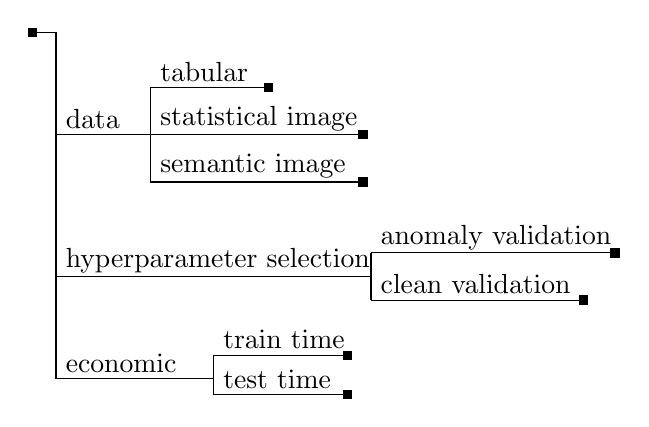
\begin{tikzpicture}
          \draw (-0.3,1.3) -- (0,1.3);
          \draw (0,1.3) -- (0,-3.1);
          
          \filldraw ([xshift=-1.5pt,yshift=-1.5pt]-0.3,1.3) rectangle ++(3pt,3pt);

          \draw (0,0) -- (1.2,0);
          \node[anchor=west] at (0,0.2) {data};
          \draw (1.2,-0.6) -- (1.2,0.6);
          \node[anchor=west] at (1.2,0.8) {tabular};
          \filldraw ([xshift=-1.5pt,yshift=-1.5pt]2.7,0.6) rectangle ++(3pt,3pt);
          \draw (1.2,0.6) -- (2.7,0.6);
          \node[anchor=west] at (1.2,0.2) {statistical image};
          \filldraw ([xshift=-1.5pt,yshift=-1.5pt]3.9,0) rectangle ++(3pt,3pt);
          \draw (1.2,0) -- (3.9,0);
          \node[anchor=west] at (1.2,-0.4) {semantic image};
          \filldraw ([xshift=-1.5pt,yshift=-1.5pt]3.9,-0.6) rectangle ++(3pt,3pt);
          \draw (1.2,-0.6) -- (3.9,-0.6);
          
          \draw (0,-1.8) -- (4,-1.8);
          \node[anchor=west] at (0,-1.6) {hyperparameter selection};
          \draw (4,-1.5) -- (4,-2.1);
          \filldraw ([xshift=-1.5pt,yshift=-1.5pt]7.1,-1.5) rectangle ++(3pt,3pt);
          \draw (4,-1.5) -- (7.1,-1.5);
          \node[anchor=west] at (4.0,-1.3) {anomaly validation};
          \filldraw ([xshift=-1.5pt,yshift=-1.5pt]6.7,-2.1) rectangle ++(3pt,3pt);
          \draw (4,-2.1) -- (6.7,-2.1);
          \node[anchor=west] at (4.0,-1.9) {clean validation};
          
          \draw (0,-3.1) -- (2,-3.1);
          \node[anchor=west] at (0,-2.9) {economic};
          \draw (2,-2.8) -- (2,-3.3);
          \filldraw ([xshift=-1.5pt,yshift=-1.5pt]3.7,-2.8) rectangle ++(3pt,3pt);
          \draw (2,-2.8) -- (3.7,-2.8);
          \node[anchor=west] at (2,-2.6) {train time};
          \filldraw ([xshift=-1.5pt,yshift=-1.5pt]3.7,-3.3) rectangle ++(3pt,3pt);
          \draw (2,-3.3) -- (3.7,-3.3);
          \node[anchor=west] at (2,-3.1) {test time};
          

    \end{tikzpicture}
    
    \caption{Various aspects of anomaly detection comparison forming the \textit{context} of the experiment.}
    \label{fig:context}
\end{figure}

While many practitioners are eager to see which method is the best for their application, the specifics of the application may differ. We have conducted a large number of experiments to identify the main sources of variability influencing the performance of anomaly detection methods. The number of combinations of these aspects is huge. Therefore, we identified the key axes of variability: datasets, hyperparameter selection strategy, and economic point of view. From these axes, we select a few discrete points, on which we will provide a comparison. The particular combination of the selected aspect will be called \emph{context}, see Fig.~\ref{fig:context} for illustration. 

The first axis is the target data domain. Our experiments used two types of datasets: \textit{tabular} and \textit{image}. This is the most obvious split, and indeed most authors of prior art test their methods on either choice of data. Another possible way to look at data is whether they contain \textit{statistical} or \textit{semantic} anomalies. Statistical anomalies should be located in areas of a low likelihood of the normal class, while semantic~\cite{ahmed2020detecting} anomalies cannot be differentiated from normal data statistically. This is because they appear in datasets with multiple sources of variations, where only some of them are considered anomalous. Such types of anomalies are most common in image datasets.  Imagine a detector that aims to learn a representation of birds from images without preprocessing. Most of the bird pictures are going to have the sky in the background. Since the background occupies most of a picture and therefore has a strong signal, a bird on grass is going to be a statistical anomaly, while an airplane with sky in the background is an example of a semantic anomaly in case the original goal was to identify pictures that do not contain a bird. The suitability of the tested methods for the dataset context axis is studied in Sec.~\ref{sec:dataset_context}.

The second axis of variability is the hyperparameter selection strategy. It should be a gold standard that the experiments are repeated on different splits of data to training, validation, and testing subsets, especially if the datasets are small. However, in most of the reviewed recent papers~\cite{liu2019generative,wang2020advae,schlegl2017unsupervised, akcay2018ganomaly, perera2019ocgan}, this procedure was not mentioned with the exception of~\cite{ruff2018deep}. Therefore, our comparison fills this gap. Also, it is important to define the nature of information available for the selection of the hyperparameters: it is indeed a very different task if there is some (often small) number of known anomalies in the validation dataset that can be used to choose hyperparameters by cross-validation or if the validation dataset is clean. In our experience, the former case is more common. Our observations are summarised in Sec.~\ref{sec:hyperparameter_context}.

The third axis is the economic aspect of a problem. There might be serious computational restrictions present in solving real-life problems. One might then not opt for a method that promises state-of-the-art performance, but for another that reaches slightly worse performance but can be trained economically, and its performance is robust with regards to hyperparameter optimization. More details on this can be found in Sec.~\ref{sec:economic_context}.

Finally, Sec.~\ref{sec:other_context} contains other influences that we have originally considered to be important but eventually did not prove to make a significant difference in comparison of multiple methods. These include the use of performance measures other than traditional AUC, the use of Bayesian optimization, and others. 

\section{Compared methods}
\label{sec:comparedmethods}
This section briefly reviews deep generative models in the order of exactness of calculation of likelihood. Therefore, it starts with flow models, continues with probabilistic (variational) autoencoders, where the prior art on the application in anomaly detection is rich, and finishes with generative adversarial networks where the calculation of any score related to likelihood is dubious at best. We specifically focus on issues that affect the performance of the method for anomaly detection, most often the anomaly score, if it is not rigorously defined. We also briefly review other examples of deep methods that are relevant for the comparison, such as two-stage models and distance-based models that are not generative but can be used in anomaly detection. We do not review classical methods here, as this has been done many times elsewhere, but we list them in the relevant experimental section.

Before the description, we introduce a notation. Training samples, $\vec{x},$ are assumed to be i.i.d from the underlying probability distribution $p({\vec{x}})$ defined on the input space $\mathcal{X}$. Following the conventional definition of an anomaly~\cite{barnett1974outliers}, each anomaly detection method is expected to provide a quantity (called score and denoted $s(\vec{x}')$) related to the probability of a sample $\vec{x}'$ being generated from $p(\vec{x}).$ The score does not need to be a normalized distribution, as the threshold is typically determined as an empirical estimate of the quantile. Most functions in this section are assumed to have parameters optimized during training. 

\subsection{Autoencoder-based models}

\paragraph{Other models and techniques}
 A plethora of models based on probabilistic autoencoders and specialized for anomaly detection was introduced in recent years, such as~\cite{zong2018deep, pereira2018unsupervised, xu2018unsupervised, principi2017acoustic, chen2018unsupervised, chalapathyGroupAnomalyDetection2018}. Below, we list models included in the comparison and not described above.

The self-adversarial Variational Autoencoder (adVAE)~\cite{wang2020advae} was included because it claims superiority over the state-of-the-art methods, such as VAE, DAGMM~\cite{zong2018deep}, WGAN-GP~\cite{gulrajani2017improved} or MO-GAAL~\cite{liu2019generative} on tabular datasets. It augments the usual encoder-decoder pair with a transformer, whose goal is to simulate anomalies during training. The seeming flaw of the model is that it is trained only on normal data, and there is no link between the real and the simulated anomalies. The sampled reconstruction is used as an anomaly score.

Despite its name, GANomaly~\cite{akcay2018ganomaly, ahnDeepGenerativeModelsBased2020} is more related to adversarial autoencoders than to GANs. It consists of encoder-decoder-encoder architecture with a discriminator, similar to an AAE. The anomaly score is the difference between latent representations of a sample after the first and second encoding. An upgrade to this model, skip-GANomaly~\cite{akcay2019skip}, uses skip connections in a U-Net type architecture. Here, the anomaly score is a combination of reconstruction error and feature-matching loss (see the next section on fmGAN). Although originally proposed only for use in images, we have implemented a variant for tabular data as well.  


\subsection{Two-stage models}
A recurring idea~\cite{ergen2017unsupervised, yaoUnsupervisedAnomalyDetection2019, ruff2018deep, vskvara2020detection} is to combine autoencoders with a secondary model acting on the latent space defined by the encoder. The motivation behind it is that the encoder should preserve the semantic information of the sample and remove noise (e.g. background in images). Additionally, reducing the size mitigates the curse of dimensionality, as high dimensions can be problematic for some models.

We are not aware of a general term for this approach. We use the term \textit{two-stage models}, following~\cite{dai2019diagnosing}, although~\cite{chalapathy2019deep} uses the term \textit{deep hybrid models}. In~\cite{ruff2018deep}, the model optimizes the projection of data (by virtue of NNs) to a new space, where they can be easily enclosed in a sphere of minimum radius. The approach presented in~\cite{vskvara2020detection, yaoUnsupervisedAnomalyDetection2019} explicitly splits the creation of the detector into two parts. It first trains a VAE (and its variants), and then it fixes the encoder. The anomaly score is calculated by a kNN \cite{vskvara2020detection} or by OC-SVM \cite{yaoUnsupervisedAnomalyDetection2019} detectors in the latent space, obtained by projecting the sample by the fixed encoder. The two-stage models can also be viewed as a kNN with a trained metric or OC-SVM with a trained kernel. The embedding can be optimized differently, for example, by enforcing the margin between anomaly candidates and normal data as done in the REPEN~\cite{pangLearningRepresentationsUltrahighdimensional2018} method, which uses an ensemble of 1NN detectors as the second stage.

\section{Experimental setup}
\label{sec:experimentalsetup}
\subsection{Datasets}

\subsection{Data splits and experiment repetitions}
\label{sec:repetitions}
The experiments on tabular data and MNIST-C/MVTec-AD image datasets were repeated five times with different random cross-validation splits. Specifically, in each repetition (five in total) of an experiment with the same model hyperparameters, the \textit{normal data} in each dataset was randomly split in 60\%/20\%/20\% ratios to train/validation/test subsets, respectively. \textit{Anomalous data} were split such that 50\% were in the validation part and 50\% in the testing part, which means the training subset has not contained anomalous samples. \footnote{A training set without any anomalies is in practice very optimistic, but this decision removes another degree of freedom from the evaluation for the sake of clarity of results.} The proportion of anomalies that were used in the validation phase varied from zero to the selected 50\%. 

Due to the already substantial computational requirements on the rest of the image datasets, we have not trained models with the same hyperparameters on repeated random cross-validation splits. In our experience, the results on different splits of these datasets are almost the same since the number of samples is large and our trial experiments (see Supplementary Tab.~\ref{tab:images_seed_consistency}) have not exhibited a significant variation between the different random cross-validation experiment repetitions. 


\subsection{Notes on implementation of models}
As mentioned in the introduction, we have compared various types of \textit{deep} methods to \emph{classical} ones serving as an etalon. Classical methods included ABOD~\cite{kriegel2008angle}, HBOS~\cite{goldstein2012histogram}, LODA~\cite{pevny2016loda}, LOF~\cite{breunig2000lof}, IsolationForest~\cite{liu2008isolation}, OC-SVM~\cite{scholkopf2001estimating}, PIDForest~\cite{gopalanPIDForestAnomalyDetection2019}, and kNN~\cite{ramaswamy2000efficient}. For ABOD, HBOS, and LODA, we have used pyOD library~\cite{zhao2019pyod} implementation, for LOF, IsolationForest, and OC-SVM we used scikit-learn~\cite{scikit-learn} implementation, and last but not least we have used our own implementation of kNN. The acronyms used in the result section are summarized in Tab.~\ref{tab:model_acronyms_2col} together with the classification of the deep methods as described in Sec.~\ref{sec:comparedmethods}.

Since image datasets are typically much larger than tabular, the OC-SVM was implemented as an ensemble of 10 OC-SVM models trained disjoint subsets of data, see Sec.~\ref{sec:appendix_implementation}, because it has at best $O(n^2)$ scaling in the number of samples. 

To ensure consistency among deep models, we implemented all methods except the MOGAAL\footnote{The pyOD implementation was used.} ourselves using the Flux~\cite{innes:2018} framework in Julia~\cite{Julia-2017} language. Apart from the models mentioned in Sec.~\ref{sec:comparedmethods}, we have also implemented DeepSVDD~\cite{ruff2018deep}, DAGMM~\cite{zong2018deep} and REPEN~\cite{pangLearningRepresentationsUltrahighdimensional2018}, which have been included in multiple comparisons~\cite{ruff2020unifying, wang2020advae, chalapathy2018anomaly}.

\begin{table}
    \centering
    \tabcolsep=0.1cm
    
    \begin{tabular}{cll|cll}
    \toprule
    \textbf{class} & \textbf{model} & \textbf{acronym} & \textbf{class} & \textbf{model} & \textbf{acronym}  \\\midrule
    
    \parbox[t]{2mm}{\multirow{3}{*}{\rotatebox[origin=c]{90}{flows}}} & MAF & maf & \parbox[t]{2mm}{\multirow{5}{*}{\rotatebox[origin=c]{90}{two-stage}}} & DAGMM & dgmm \\
        & RealNVP & rnvp & & DeepSVDD & dsvd \\
        & SPTN & sptn & & REPEN & rpn  \\
        & & & & VAE-kNN & vaek \\

    \parbox[t]{2mm}{\multirow{5}{*}{\rotatebox[origin=c]{90}{autoencoders}}} 
        & AAE & aae & & VAE-OC-SVM & vaeo \\
        & adVAE & avae & & & \\

        & GANomaly & gano & \parbox[t]{2mm}{\multirow{8}{*}{\rotatebox[origin=c]{90}{classical}}} & ABOD & abod \\

        & skipGANomaly & skip & & HBOS & hbos \\
        & VAE & vae & & IsolationForest & if \\
        & WAE & wae & & kNN & knn \\
        & & & & LODA & loda \\
    \parbox[t]{2mm}{\multirow{3}{*}{\rotatebox[origin=c]{90}{gans}}}
        & fAnoGAN & fano & & LOF & lof \\ 
        & fmGAN & fmgn & & OC-SVM & osvm \\
        & GAN & gan & & PidForest & pidf \\
        & MOGAAL & mgal & \\
    
    \bottomrule
    \end{tabular}

    \vspace*{0.15cm}
    \caption{Overview of the main classes of compared methods and the acronyms used in the text.}
    \label{tab:model_acronyms_2col}
\end{table}

We emphasize that while implementing models, we have carefully compared our implementations to the reference where possible and (or) verified that our experimental results are similar to those provided in the corresponding publication.

Neural networks were trained with the ADAM~\cite{kingma2014adam} optimizer with early stopping measuring the continued decrease of loss on the validation dataset. All deep models trained on all image datasets used convolutional layers. More implementation details are in the Supplementary materials Sec.~\ref{sec:appendix_implementation}. The implementation code in the form of a Julia package can be found at \textbf{https://github.com/aicenter/GenerativeAD.jl}.

\subsection{Hyperparameters and their optimization}
\label{sub:hyperparameteroptimization}
Properly exploring the space of hyperparameters of all models is paramount to achieving fair and comparable experimental comparison, yet this is often superficially treated. Researchers often use \textit{default} or \textit{recommended} values ignoring that they are sub-optimal on datasets they use in their comparison. The conflicting results of the MOGAAL method in the original publication~\cite{liu2019generative} and in~\cite{wang2020advae} are a nice demonstration of this.  A prototypical example in the classical methods is OC-SVM, which is typically used with Gaussian kernel and with $\nu$ set to some default value, e.g. 0.05~\cite{pevny2016loda}, but can achieve better results with different kernels. The choice of hyperparameters in anomaly detection is everything but easy. But this means that the experimental settings should be set up such that all methods have been optimized equally. We conjecture that recommended and default values of hyperparameters are strongly correlated with the choice of evaluation datasets in the publications that recommend them.

\textit{Random grid search:} In order to explore the hyperparameter space of each method properly, we have employed a random search over a predefined grid for each method. This allows the construction of sections through the space for sensitivity studies. Moreover, it is frequently more efficient than grid search~\cite{bergstra2012random} and more flexible. For each model, dataset, and repetition, we have sampled 100 configurations from corresponding sets (see Tab.~\ref{tab:classical_hyperparameters}--\ref{tab:flow_hyperparameters}) and trained the models with them. In order to keep the neural-network-based models fixed across the repetitions on a single dataset, for each hyperparameter configuration we have also sampled a random seed that was used to initialize the network weights. To prevent running the training of expensive methods forever, there was a hard deadline of 24 hours in which the training of a single configuration for a given number of repetitions/classes should be finished. This automatically penalizes complicated models. 

Encoders for the two-stage models were selected from models performing best in terms of validation AUC or reconstruction error on the validation set. The second-stage models (kNN and OC-SVM) used hyperparameters sampled from Tab.~\ref{tab:classical_hyperparameters}. 

\textit{Bayesian optimization:} To overcome the limitation of random sampling in larger configuration spaces, we have also trained models whose hyperparameter choice was guided by Bayesian optimization of an evaluation metric on validation data. We followed the 50/50 strategy, where the underlying Gaussian process has been fitted with 50 randomly sampled configurations, and another 50 have been sampled based on the acquisition function. We have relied on the off-the-shelf implementation from the scikit-optimize framework~\cite{skopt} with default parameters.

\textit{Number of anomalies in the validation set:} A thorough exploration of the hyperparameter selection context also requires changing the criteria of model selection. When anomalies are available for validation, we select hyperparameters maximizing the AUC on the validation set. For experiments with no available anomalies, we have decided on the following hyperparameter selection mechanism. For \textit{classical} methods, we have used default hyperparameter values from literature - either authors of the method recommended them, they were used in a survey, or are default in a given implementation. Their overview is in Tab.~\ref{tab:default_hyperparameters}. For \textit{deep} methods, this is unfortunately impossible since their hyperparameter space is much larger, and the values are usually tuned to a specific dataset. Therefore, to have a universal solution, we have selected the already trained and evaluated models based on the lowest anomaly score on the normal validation data. This approach is theoretically justified for models with proper likelihood. 

\textit{Ensembles:} Some results on ensembles of anomaly detectors were already reported in~\cite{choiWAICWhyGenerative2019, nalisnickDeepGenerativeModels2019}. Since the other experiments required training a large number of models, it was decided to test whether even a naive approach to this problem brings some improvements. In order to mitigate some uncertainty given by different hyperparameter values, ensembles of detectors were constructed by averaging scores of some number of best-performing detectors. We have experimented with different fixed sizes of ensembles --- either top 10 or top 5. In such a case, the anomaly score is the average of the anomaly scores of ensemble members.

\textit{Performance criteria:} While the area under the ROC curve (AUC) is the most common criteria in anomaly detection, some authors use different metrics, such as partial AUC~\cite{dodd2003partial} or the true positive rate at a chosen false negative rate (TPR@). We have re-evaluated all results obtained for the random grid search on the TPR@5\%.

We have kept track of the time spent on the training of individual models and also on the time needed to evaluate them on validation and test sets. In total, we have trained 1,364,989 model instances in 9619 CPU days, evaluated 4,256,470 different scoring functions in 2704 CPU days, and created 10.2TB of experimental data.

\section{Experimental results}
\label{sec:results}
Before starting with the description of the experimental results, here we summarize conventions that are used unless said otherwise. The performance results are estimates of the AUC on the testing set and are averaged over five random cross-validation repetitions in the case of tabular and MvTec-AD/MNISTC image datasets. When ranks are reported, they are calculated by ordering methods on each dataset and calculating the average across them (as recommended in~\cite{demvsar2006statistical}). Hyperparameters are selected using the best average performance over 5 seeds or individually over 10 anomaly classes because the individual class splits constitute different anomaly detection problems. 

\begin{figure*}[h]
    \begin{tabular}{c c}
    \resizebox{\columnwidth}{!}{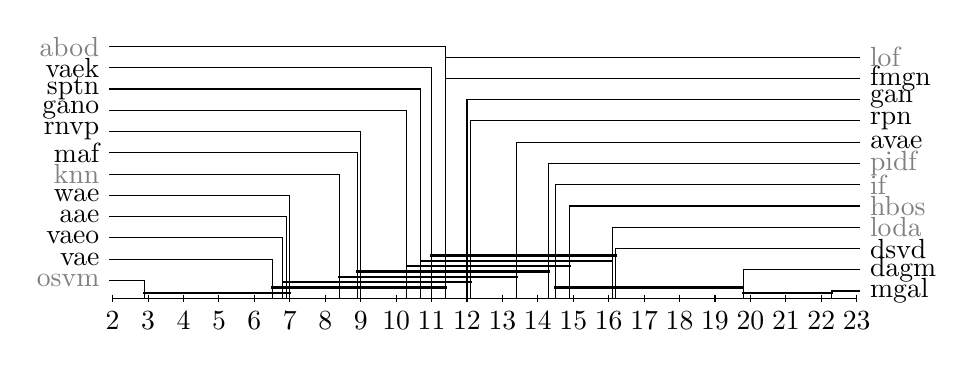
\begin{tikzpicture}[scale=0.45] 
  \draw (2.0,0) -- (23.0,0); 
  \foreach \x in {2,...,23} \draw (\x,0.10) -- (\x,-0.10) node[anchor=north]{$\x$}; 
  \draw (2.9,0) -- (2.9,0.5) -- (1.9, 0.5) node[anchor=east] {\textcolor{gray}{osvm}}; 
  \draw (6.5,0) -- (6.5,1.0999999999999999) -- (1.9, 1.0999999999999999) node[anchor=east] {vae}; 
  \draw (6.8,0) -- (6.8,1.6999999999999997) -- (1.9, 1.6999999999999997) node[anchor=east] {vaeo}; 
  \draw (6.9,0) -- (6.9,2.3) -- (1.9, 2.3) node[anchor=east] {aae}; 
  \draw (7.0,0) -- (7.0,2.9) -- (1.9, 2.9) node[anchor=east] {wae}; 
  \draw (8.4,0) -- (8.4,3.4999999999999996) -- (1.9, 3.4999999999999996) node[anchor=east] {\textcolor{gray}{knn}}; 
  \draw (8.9,0) -- (8.9,4.1000000000000005) -- (1.9, 4.1000000000000005) node[anchor=east] {maf}; 
  \draw (9.0,0) -- (9.0,4.7) -- (1.9, 4.7) node[anchor=east] {rnvp}; 
  \draw (10.3,0) -- (10.3,5.3) -- (1.9, 5.3) node[anchor=east] {gano}; 
  \draw (10.7,0) -- (10.7,5.9) -- (1.9, 5.9) node[anchor=east] {sptn}; 
  \draw (11.0,0) -- (11.0,6.5) -- (1.9, 6.5) node[anchor=east] {vaek}; 
  \draw (11.4,0) -- (11.4,7.1) -- (1.9, 7.1) node[anchor=east] {\textcolor{gray}{abod}}; 
  \draw (11.4,0) -- (11.4,6.8) -- (23.1, 6.8) node[anchor=west] {\textcolor{gray}{lof}}; 
  \draw (11.4,0) -- (11.4,6.2) -- (23.1, 6.2) node[anchor=west] {fmgn}; 
  \draw (12.0,0) -- (12.0,5.6) -- (23.1, 5.6) node[anchor=west] {gan}; 
  \draw (12.1,0) -- (12.1,5.0) -- (23.1, 5.0) node[anchor=west] {rpn}; 
  \draw (13.4,0) -- (13.4,4.4) -- (23.1, 4.4) node[anchor=west] {avae}; 
  \draw (14.3,0) -- (14.3,3.8) -- (23.1, 3.8) node[anchor=west] {\textcolor{gray}{pidf}}; 
  \draw (14.5,0) -- (14.5,3.2) -- (23.1, 3.2) node[anchor=west] {\textcolor{gray}{if}}; 
  \draw (14.9,0) -- (14.9,2.6) -- (23.1, 2.6) node[anchor=west] {\textcolor{gray}{hbos}}; 
  \draw (16.1,0) -- (16.1,1.9999999999999998) -- (23.1, 1.9999999999999998) node[anchor=west] {\textcolor{gray}{loda}}; 
  \draw (16.2,0) -- (16.2,1.4) -- (23.1, 1.4) node[anchor=west] {dsvd}; 
  \draw (19.8,0) -- (19.8,0.8) -- (23.1, 0.8) node[anchor=west] {dagm}; 
  \draw (22.3,0) -- (22.3,0.2) -- (23.1, 0.2) node[anchor=west] {mgal}; 
  \draw[line width=0.03cm,color=black,draw opacity=1.0] (2.87,0.15) -- (7.03,0.15); 
  \draw[line width=0.03cm,color=black,draw opacity=1.0] (6.47,0.3) -- (11.43,0.3); 
  \draw[line width=0.03cm,color=black,draw opacity=1.0] (6.77,0.44999999999999996) -- (12.129999999999999,0.44999999999999996); 
  \draw[line width=0.03cm,color=black,draw opacity=1.0] (8.370000000000001,0.6) -- (13.43,0.6); 
  \draw[line width=0.03cm,color=black,draw opacity=1.0] (8.870000000000001,0.75) -- (14.33,0.75); 
  \draw[line width=0.03cm,color=black,draw opacity=1.0] (10.270000000000001,0.9) -- (14.93,0.9); 
  \draw[line width=0.03cm,color=black,draw opacity=1.0] (10.67,1.05) -- (16.130000000000003,1.05); 
  \draw[line width=0.03cm,color=black,draw opacity=1.0] (10.97,1.2) -- (16.23,1.2); 
  \draw[line width=0.03cm,color=black,draw opacity=1.0] (14.47,0.3) -- (19.830000000000002,0.3); 
  \draw[line width=0.03cm,color=black,draw opacity=1.0] (19.77,0.15) -- (22.330000000000002,0.15); 
 \end{tikzpicture} 
} & \resizebox{\columnwidth}{!}{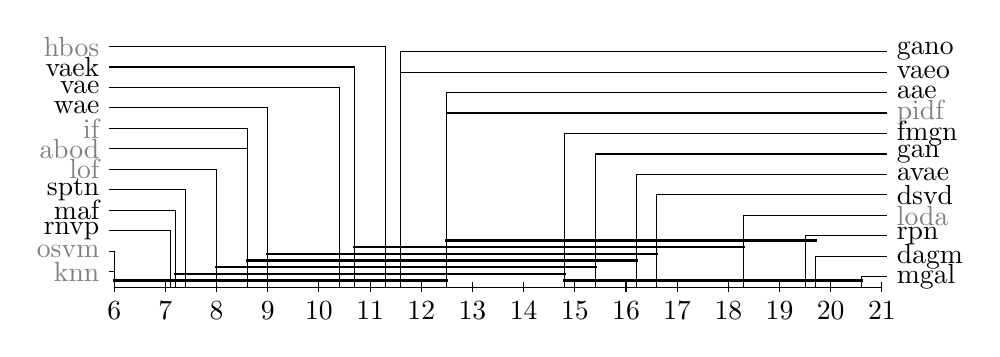
\begin{tikzpicture}[scale=0.65] 
  \draw (6.0,0) -- (21.0,0); 
  \foreach \x in {6,...,21} \draw (\x,0.10) -- (\x,-0.10) node[anchor=north]{$\x$}; 
  \draw (6.0,0) -- (6.0,0.30000000000000004) -- (5.9, 0.30000000000000004) node[anchor=east] {\textcolor{gray}{knn}}; 
  \draw (6.0,0) -- (6.0,0.7000000000000001) -- (5.9, 0.7000000000000001) node[anchor=east] {\textcolor{gray}{osvm}}; 
  \draw (7.1,0) -- (7.1,1.1) -- (5.9, 1.1) node[anchor=east] {rnvp}; 
  \draw (7.2,0) -- (7.2,1.5) -- (5.9, 1.5) node[anchor=east] {maf}; 
  \draw (7.4,0) -- (7.4,1.9) -- (5.9, 1.9) node[anchor=east] {sptn}; 
  \draw (8.0,0) -- (8.0,2.3000000000000003) -- (5.9, 2.3000000000000003) node[anchor=east] {\textcolor{gray}{lof}}; 
  \draw (8.6,0) -- (8.6,2.7) -- (5.9, 2.7) node[anchor=east] {\textcolor{gray}{abod}}; 
  \draw (8.6,0) -- (8.6,3.1) -- (5.9, 3.1) node[anchor=east] {\textcolor{gray}{if}}; 
  \draw (9.0,0) -- (9.0,3.5) -- (5.9, 3.5) node[anchor=east] {wae}; 
  \draw (10.4,0) -- (10.4,3.9) -- (5.9, 3.9) node[anchor=east] {vae}; 
  \draw (10.7,0) -- (10.7,4.300000000000001) -- (5.9, 4.300000000000001) node[anchor=east] {vaek}; 
  \draw (11.3,0) -- (11.3,4.700000000000001) -- (5.9, 4.700000000000001) node[anchor=east] {\textcolor{gray}{hbos}}; 
  \draw (11.6,0) -- (11.6,4.6000000000000005) -- (21.1, 4.6000000000000005) node[anchor=west] {gano}; 
  \draw (11.6,0) -- (11.6,4.2) -- (21.1, 4.2) node[anchor=west] {vaeo}; 
  \draw (12.5,0) -- (12.5,3.8000000000000003) -- (21.1, 3.8000000000000003) node[anchor=west] {aae}; 
  \draw (12.5,0) -- (12.5,3.4000000000000004) -- (21.1, 3.4000000000000004) node[anchor=west] {\textcolor{gray}{pidf}}; 
  \draw (14.8,0) -- (14.8,3.0000000000000004) -- (21.1, 3.0000000000000004) node[anchor=west] {fmgn}; 
  \draw (15.4,0) -- (15.4,2.6000000000000005) -- (21.1, 2.6000000000000005) node[anchor=west] {gan}; 
  \draw (16.2,0) -- (16.2,2.2) -- (21.1, 2.2) node[anchor=west] {avae}; 
  \draw (16.6,0) -- (16.6,1.8) -- (21.1, 1.8) node[anchor=west] {dsvd}; 
  \draw (18.3,0) -- (18.3,1.4000000000000001) -- (21.1, 1.4000000000000001) node[anchor=west] {\textcolor{gray}{loda}}; 
  \draw (19.5,0) -- (19.5,1.0) -- (21.1, 1.0) node[anchor=west] {rpn}; 
  \draw (19.7,0) -- (19.7,0.6000000000000001) -- (21.1, 0.6000000000000001) node[anchor=west] {dagm}; 
  \draw (20.6,0) -- (20.6,0.2) -- (21.1, 0.2) node[anchor=west] {mgal}; 
  \draw[line width=0.03cm,color=black,draw opacity=1.0] (5.97,0.13) -- (12.53,0.13); 
  \draw[line width=0.03cm,color=black,draw opacity=1.0] (7.17,0.26) -- (14.83,0.26); 
  \draw[line width=0.03cm,color=black,draw opacity=1.0] (7.97,0.39) -- (15.43,0.39); 
  \draw[line width=0.03cm,color=black,draw opacity=1.0] (8.57,0.52) -- (16.23,0.52); 
  \draw[line width=0.03cm,color=black,draw opacity=1.0] (8.97,0.65) -- (16.630000000000003,0.65); 
  \draw[line width=0.03cm,color=black,draw opacity=1.0] (10.67,0.78) -- (18.330000000000002,0.78); 
  \draw[line width=0.03cm,color=black,draw opacity=1.0] (12.47,0.91) -- (19.73,0.91); 
  \draw[line width=0.03cm,color=black,draw opacity=1.0] (14.770000000000001,0.13) -- (20.630000000000003,0.13); 
 \end{tikzpicture} 
} \\
    a) tabular datasets, anomaly validation & b) tabular datasets, clean validation \\  
    \resizebox{\columnwidth}{!}{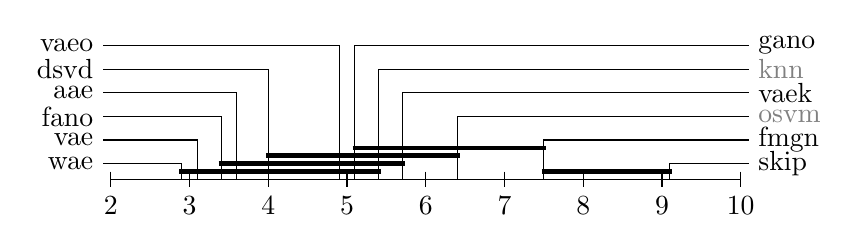
\begin{tikzpicture}[scale=1.0] 
  \draw (2.0,0) -- (10.0,0); 
  \foreach \x in {2,...,10} \draw (\x,0.10) -- (\x,-0.10) node[anchor=north]{$\x$}; 
  \draw (2.9,0) -- (2.9,0.19999999999999998) -- (1.9, 0.19999999999999998) node[anchor=east] {wae}; 
  \draw (3.1,0) -- (3.1,0.5) -- (1.9, 0.5) node[anchor=east] {vae}; 
  \draw (3.4,0) -- (3.4,0.7999999999999999) -- (1.9, 0.7999999999999999) node[anchor=east] {fano}; 
  \draw (3.6,0) -- (3.6,1.0999999999999999) -- (1.9, 1.0999999999999999) node[anchor=east] {aae}; 
  \draw (4.0,0) -- (4.0,1.4) -- (1.9, 1.4) node[anchor=east] {dsvd}; 
  \draw (4.9,0) -- (4.9,1.6999999999999997) -- (1.9, 1.6999999999999997) node[anchor=east] {vaeo}; 
  \draw (5.1,0) -- (5.1,1.7) -- (10.1, 1.7) node[anchor=west] {gano}; 
  \draw (5.4,0) -- (5.4,1.4) -- (10.1, 1.4) node[anchor=west] {\textcolor{gray}{knn}}; 
  \draw (5.7,0) -- (5.7,1.0999999999999999) -- (10.1, 1.0999999999999999) node[anchor=west] {vaek}; 
  \draw (6.4,0) -- (6.4,0.8) -- (10.1, 0.8) node[anchor=west] {\textcolor{gray}{osvm}}; 
  \draw (7.5,0) -- (7.5,0.5) -- (10.1, 0.5) node[anchor=west] {fmgn}; 
  \draw (9.1,0) -- (9.1,0.2) -- (10.1, 0.2) node[anchor=west] {skip}; 
  \draw[line width=0.06cm,color=black,draw opacity=1.0] (2.87,0.1) -- (5.430000000000001,0.1); 
  \draw[line width=0.06cm,color=black,draw opacity=1.0] (3.37,0.2) -- (5.73,0.2); 
  \draw[line width=0.06cm,color=black,draw opacity=1.0] (3.97,0.30000000000000004) -- (6.430000000000001,0.30000000000000004); 
  \draw[line width=0.06cm,color=black,draw opacity=1.0] (5.069999999999999,0.4) -- (7.53,0.4); 
  \draw[line width=0.06cm,color=black,draw opacity=1.0] (7.47,0.1) -- (9.129999999999999,0.1); 
 \end{tikzpicture} 
} & \resizebox{\columnwidth}{!}{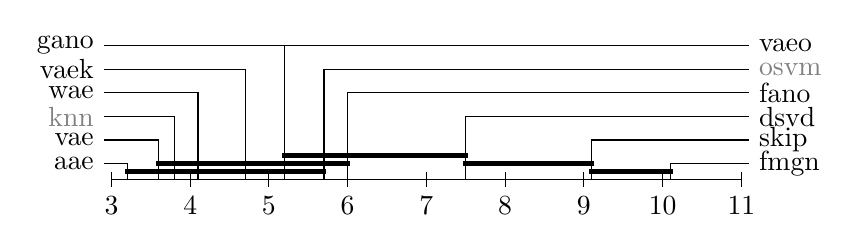
\begin{tikzpicture}[scale=1.0] 
  \draw (3.0,0) -- (11.0,0); 
  \foreach \x in {3,...,11} \draw (\x,0.10) -- (\x,-0.10) node[anchor=north]{$\x$}; 
  \draw (3.2,0) -- (3.2,0.19999999999999998) -- (2.9, 0.19999999999999998) node[anchor=east] {aae}; 
  \draw (3.6,0) -- (3.6,0.5) -- (2.9, 0.5) node[anchor=east] {vae}; 
  \draw (3.8,0) -- (3.8,0.7999999999999999) -- (2.9, 0.7999999999999999) node[anchor=east] {\textcolor{gray}{knn}}; 
  \draw (4.1,0) -- (4.1,1.0999999999999999) -- (2.9, 1.0999999999999999) node[anchor=east] {wae}; 
  \draw (4.7,0) -- (4.7,1.4) -- (2.9, 1.4) node[anchor=east] {vaek}; 
  \draw (5.2,0) -- (5.2,1.6999999999999997) -- (2.9, 1.6999999999999997) node[anchor=east] {gano}; 
  \draw (5.2,0) -- (5.2,1.7) -- (11.1, 1.7) node[anchor=west] {vaeo}; 
  \draw (5.7,0) -- (5.7,1.4) -- (11.1, 1.4) node[anchor=west] {\textcolor{gray}{osvm}}; 
  \draw (6.0,0) -- (6.0,1.0999999999999999) -- (11.1, 1.0999999999999999) node[anchor=west] {fano}; 
  \draw (7.5,0) -- (7.5,0.8) -- (11.1, 0.8) node[anchor=west] {dsvd}; 
  \draw (9.1,0) -- (9.1,0.5) -- (11.1, 0.5) node[anchor=west] {skip}; 
  \draw (10.1,0) -- (10.1,0.2) -- (11.1, 0.2) node[anchor=west] {fmgn}; 
  \draw[line width=0.06cm,color=black,draw opacity=1.0] (3.1700000000000004,0.1) -- (5.73,0.1); 
  \draw[line width=0.06cm,color=black,draw opacity=1.0] (3.5700000000000003,0.2) -- (6.03,0.2); 
  \draw[line width=0.06cm,color=black,draw opacity=1.0] (5.17,0.30000000000000004) -- (7.53,0.30000000000000004); 
  \draw[line width=0.06cm,color=black,draw opacity=1.0] (7.47,0.2) -- (9.129999999999999,0.2); 
  \draw[line width=0.06cm,color=black,draw opacity=1.0] (9.07,0.1) -- (10.129999999999999,0.1); 
 \end{tikzpicture} 
}\\
    c) statistical image datasets, anomaly validation & d) statistical image  datasets, clean validation \\ 
     \resizebox{\columnwidth}{!}{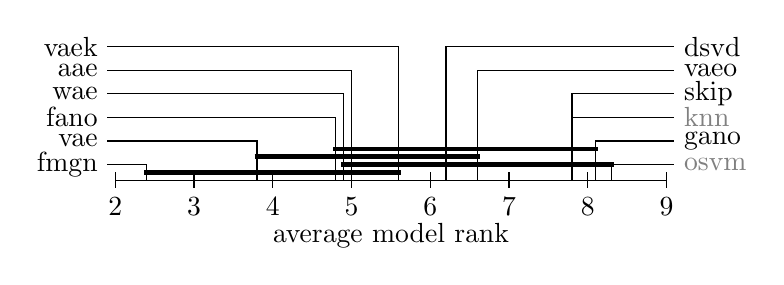
\begin{tikzpicture}[scale=1.0] 
  \draw (2.0,0) -- (9.0,0); 
  \foreach \x in {2,...,9} \draw (\x,0.10) -- (\x,-0.10) node[anchor=north]{$\x$}; 
  \draw (2.4,0) -- (2.4,0.19999999999999998) -- (1.9, 0.19999999999999998) node[anchor=east] {fmgn}; 
  \draw (3.8,0) -- (3.8,0.5) -- (1.9, 0.5) node[anchor=east] {vae}; 
  \draw (4.8,0) -- (4.8,0.7999999999999999) -- (1.9, 0.7999999999999999) node[anchor=east] {fano}; 
  \draw (4.9,0) -- (4.9,1.0999999999999999) -- (1.9, 1.0999999999999999) node[anchor=east] {wae}; 
  \draw (5.0,0) -- (5.0,1.4) -- (1.9, 1.4) node[anchor=east] {aae}; 
  \draw (5.6,0) -- (5.6,1.6999999999999997) -- (1.9, 1.6999999999999997) node[anchor=east] {vaek}; 
  \draw (6.2,0) -- (6.2,1.7) -- (9.1, 1.7) node[anchor=west] {dsvd}; 
  \draw (6.6,0) -- (6.6,1.4) -- (9.1, 1.4) node[anchor=west] {vaeo}; 
  \draw (7.8,0) -- (7.8,1.0999999999999999) -- (9.1, 1.0999999999999999) node[anchor=west] {skip}; 
  \draw (7.8,0) -- (7.8,0.8) -- (9.1, 0.8) node[anchor=west] {\textcolor{gray}{knn}}; 
  \draw (8.1,0) -- (8.1,0.5) -- (9.1, 0.5) node[anchor=west] {gano}; 
  \draw (8.3,0) -- (8.3,0.2) -- (9.1, 0.2) node[anchor=west] {\textcolor{gray}{osvm}}; 
  \draw[line width=0.06cm,color=black,draw opacity=1.0] (2.37,0.1) -- (5.63,0.1); 
  \draw[line width=0.06cm,color=black,draw opacity=1.0] (3.77,0.3) -- (6.63,0.3); 
  \draw[line width=0.06cm,color=black,draw opacity=1.0] (4.77,0.4) -- (8.129999999999999,0.4); 
  \draw[line width=0.06cm,color=black,draw opacity=1.0] (4.87,0.2) -- (8.33,0.2); 
  \node[anchor=center] at (5.5,-0.7) {average model rank};
 \end{tikzpicture} 
} & \resizebox{\columnwidth}{!}{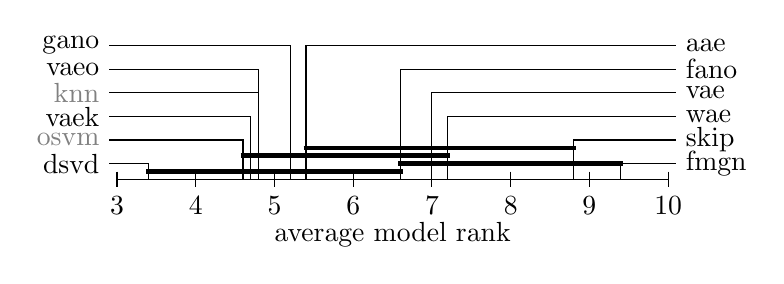
\begin{tikzpicture}[scale=1.0] 
  \draw (3.0,0) -- (10.0,0); 
  \foreach \x in {3,...,10} \draw (\x,0.10) -- (\x,-0.10) node[anchor=north]{$\x$}; 
  \draw (3.4,0) -- (3.4,0.19999999999999998) -- (2.9, 0.19999999999999998) node[anchor=east] {dsvd}; 
  \draw (4.6,0) -- (4.6,0.5) -- (2.9, 0.5) node[anchor=east] {\textcolor{gray}{osvm}}; 
  \draw (4.7,0) -- (4.7,0.7999999999999999) -- (2.9, 0.7999999999999999) node[anchor=east] {vaek}; 
  \draw (4.8,0) -- (4.8,1.0999999999999999) -- (2.9, 1.0999999999999999) node[anchor=east] {\textcolor{gray}{knn}}; 
  \draw (4.8,0) -- (4.8,1.4) -- (2.9, 1.4) node[anchor=east] {vaeo}; 
  \draw (5.2,0) -- (5.2,1.6999999999999997) -- (2.9, 1.6999999999999997) node[anchor=east] {gano}; 
  \draw (5.4,0) -- (5.4,1.7) -- (10.1, 1.7) node[anchor=west] {aae}; 
  \draw (6.6,0) -- (6.6,1.4) -- (10.1, 1.4) node[anchor=west] {fano}; 
  \draw (7.0,0) -- (7.0,1.0999999999999999) -- (10.1, 1.0999999999999999) node[anchor=west] {vae}; 
  \draw (7.2,0) -- (7.2,0.8) -- (10.1, 0.8) node[anchor=west] {wae}; 
  \draw (8.8,0) -- (8.8,0.5) -- (10.1, 0.5) node[anchor=west] {skip}; 
  \draw (9.4,0) -- (9.4,0.2) -- (10.1, 0.2) node[anchor=west] {fmgn}; 
  \draw[line width=0.06cm,color=black,draw opacity=1.0] (3.37,0.1) -- (6.63,0.1); 
  \draw[line width=0.06cm,color=black,draw opacity=1.0] (4.569999999999999,0.3) -- (7.23,0.3); 
  \draw[line width=0.06cm,color=black,draw opacity=1.0] (5.37,0.4) -- (8.83,0.4); 
  \draw[line width=0.06cm,color=black,draw opacity=1.0] (6.569999999999999,0.2) -- (9.43,0.2); 
  \node[anchor=center] at (6.5,-0.7) {average model rank};
 \end{tikzpicture} 
} \\
    e) semantic image  datasets, anomaly validation & f) semantic image datasets, clean validation \\
    \end{tabular}
 \caption{Critical difference diagram of models ranked via the test AUC. Models whose performance is statistically indistinguishable have a difference of ranks under the critical value of the Nemenyi test $CD_{0.1}$ and are joined by a horizontal band. Results are presented for different types of datasets: tabular (Top row), image datasets with statistical anomalies (Middle row), and image datasets with semantic anomalies (Bottom row); and two different hyperparameter selection cases: using anomalies in validation (left) and using clean validation (right).
 }
 % $CD_{0.05}(24, 40) = 5.75$
 \label{fig:critical_diag}
\end{figure*}

\subsection{Dataset context}
\label{sec:dataset_context}
The results of experimental comparison on all dataset types are presented in the form of critical difference diagrams (CDD) as recommended by Dem\v{s}ar~\cite{demvsar2006statistical}, are in Fig.~\ref{fig:critical_diag}. Diagrams show the average rank of detectors across the datasets together with a confidence band that indicates that a statistical test cannot reject the hypothesis that two detectors perform the same. The underlying  AUC values on the testing set for all individual datasets are given in Tab.~\ref{tab:tabular_anomalies}, \ref{tab:tabular_clean}, \ref{tab:images_stat_auc_auc_combined}, and~\ref{tab:images_semantic_auc_auc_combined}. We now comment on the influence of the datatype with respect to two types of hyperparameter selection strategies differing in the number of anomalies in the validation set as defined in Section~\ref{sec:contexts}: i) anomaly validation context, and ii) clean validation context.

\emph{Tabular data:} OC-SVM works the best and it is \emph{statistically better} than almost all detectors except autoencoder-based generative models and VAE combined with OC-SVM in the case of anomaly validation context. The first 11 places (roughly one half) belong to models that can be divided into three groups: (i) OC-SVM and its variants, which estimate a density level of a distribution; (ii) flow models and kNN, which estimate the pdf (un-normalized in case of kNN); (iii) and variants of auto-encoders, where reconstruction error is related to pdf as explained in~\cite{vsmidl2019anomaly}. The same types of methods occupy the top positions in the clean validation context, Fig.~\ref{fig:critical_diag}b), however in a different order. The best is the kNN, and all other pdf-modeling methods (flows) have improved relative to the anomaly validation context. The autoencoder-based methods moved beyond classical methods (LOF, ABOD, IF). We believe that models in the lower half of the scale in both validation contexts are not suitable for detecting statistical anomalies. We cannot explain the poor performance of MOGAAL, DAGMM, and adVAE,\footnote{We have contacted the author of pyOD from wherein we took the implementation of MOGAAL, and we were assured that his implementation is a copy of that provided by the authors. Therefore, we consider the implementation to be correct.} and we attribute it to different experimental environment. DeepSVDD was primarily implemented for image problems, where it performs relatively well.

Moreover, differences in mean ranks of many models in Fig.~\ref{fig:critical_diag} are statistically insignificant at level $p=0.1$, which is disappointing. Assuming the ranks remain the same, another 51 datasets would be needed to make the difference between OC-SVM and VAE statistically significant on tabular data with 50\% anomalies. This indicates that the results are still noisy and can be easily changed for a different choice of datasets.

\emph{Statistical image data:} WAE and VAE models have the best average rank when evaluated on statistical image data, although their lead is not statistically significant over most of the other models as is evident from Fig.~\ref{fig:critical_diag}c). The autoencoder-based methods (AAE,VAE,WAE) perform well also in the clean validation context, complemented by kNN, Fig.~\ref{fig:critical_diag}d).

\emph{Semantic image data}
A different story is told by Fig.~\ref{fig:critical_diag}e) where the ranking of methods on image datasets with semantic anomalies is dominated by fmGAN by a large margin in the anomaly validation context. However, it is also the worst method in the clean validation context. In an opposite manner, 
OC-SVM and kNN perform very poorly in the anomaly validation context, but they are among the best in the clean validation context.  The best performing method in the clean validation context is DeepSVDD~\cite{ruff2018deep}. We conjecture that the performance of the fmGAN is related to the variability of its training. With a sufficient number of anomalies in the validation set, it is possible to find one trained model that fits the problem.

The typical anomalies detected by various methods on image datasets are provided in the Supplementary \ref{sec:appendix_extending_image_results}.


\subsection{Hyperparameter selection context}
\label{sec:hyperparameter_context}
The influence of the hyperparameter selection procedure on the results in the previous section is now studied in detail for few selected methods. We choose only those that scored among the best in the previous section. First, we analyze the sensitivity of these methods to the number of anomalies in the validation set. Second, we study hyperparameter selection for two individual methods, variational autoencoder family and OC-SVM.

\subsubsection{Impact of the number of anomalies in the validation set}
\begin{figure*}[hbt!]
    \centering
    % \footnotesize
    % \resizebox {\linewidth}{!}{
    % \input{data/chapter_comparison/combined_knowledge_rank_pat_auc_repre_mvc}
    % \input{data/chapter_comparison/combined_knowledge_rank_pat_auc_repre_mvc_per_ac}
    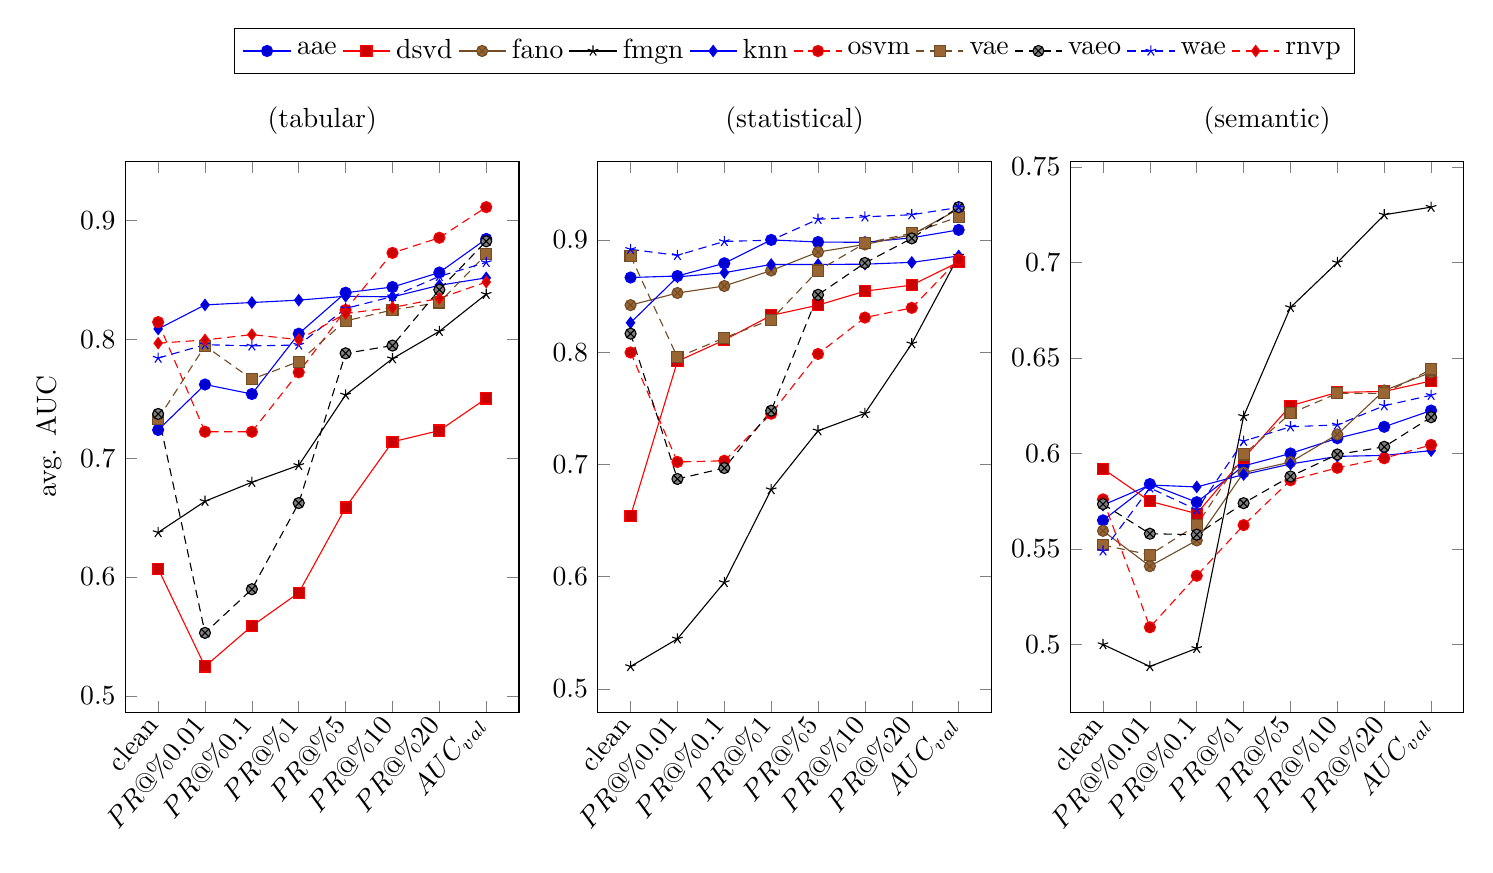
\begin{tikzpicture}[]
\begin{groupplot}[group style={vertical sep = 0.5cm, horizontal sep = 1.0cm, group size=3 by 1}]

\nextgroupplot [
  % legend style = {at={(0.3,1.30)}, anchor=west},
  ylabel = {avg. AUC},
  width=5cm, height=7cm, scale only axis=true, 
  xtick={1,2,3,4,5,6,7,8}, 
  xticklabels={clean,$PR@\%0.01$,$PR@\%0.1$,$PR@\%1$,$PR@\%5$,$PR@\%10$,$PR@\%20$,$AUC_{val}$},
  width=5cm, height=7cm, scale only axis=true,
  x tick label style={rotate=50,anchor=east},
  title = {(tabular)},
  % title style={at={(current bounding box.north)}, anchor=west},
]

\addplot+ coordinates {
  (1.0, 0.72375)
  (2.0, 0.762)
  (3.0, 0.754)
  (4.0, 0.8047500000000001)
  (5.0, 0.83925)
  (6.0, 0.844)
  (7.0, 0.8562500000000002)
  (8.0, 0.8845000000000001)
};

\addplot+ coordinates {
  (1.0, 0.607)
  (2.0, 0.52475)
  (3.0, 0.5587500000000001)
  (4.0, 0.5867500000000001)
  (5.0, 0.6585)
  (6.0, 0.71375)
  (7.0, 0.7232500000000001)
  (8.0, 0.7502500000000001)
};

\addplot+ coordinates {};

\addplot+ coordinates {
  (1.0, 0.6375)
  (2.0, 0.66375)
  (3.0, 0.6797500000000001)
  (4.0, 0.6940000000000001)
  (5.0, 0.75325)
  (6.0, 0.7837500000000001)
  (7.0, 0.8067500000000001)
  (8.0, 0.8380000000000001)
};

\addplot+ coordinates {
  (1.0, 0.8087500000000002)
  (2.0, 0.8290000000000001)
  (3.0, 0.8310000000000001)
  (4.0, 0.8329999999999999)
  (5.0, 0.8362499999999999)
  (6.0, 0.8357499999999998)
  (7.0, 0.8454999999999998)
  (8.0, 0.8517499999999998)
};

\addplot+ coordinates {
  (1.0, 0.8145)
  (2.0, 0.7222500000000001)
  (3.0, 0.7222500000000001)
  (4.0, 0.77225)
  (5.0, 0.8247500000000001)
  (6.0, 0.8727499999999999)
  (7.0, 0.8854999999999998)
  (8.0, 0.9112500000000001)
};

\addplot+ coordinates {
  (1.0, 0.7329999999999999)
  (2.0, 0.7945)
  (3.0, 0.7665)
  (4.0, 0.7812500000000001)
  (5.0, 0.8154999999999999)
  (6.0, 0.8247499999999999)
  (7.0, 0.8310000000000001)
  (8.0, 0.8714999999999999)
};

\addplot+ coordinates {
  (1.0, 0.7372500000000001)
  (2.0, 0.5530000000000002)
  (3.0, 0.5897500000000002)
  (4.0, 0.6622499999999999)
  (5.0, 0.7882499999999999)
  (6.0, 0.79475)
  (7.0, 0.84175)
  (8.0, 0.8825)
};

\addplot+ coordinates {
  (1.0, 0.7842499999999999)
  (2.0, 0.7955000000000002)
  (3.0, 0.7945)
  (4.0, 0.79525)
  (5.0, 0.826)
  (6.0, 0.836)
  (7.0, 0.853)
  (8.0, 0.8647499999999999)
};

\addplot+ coordinates {
  (1.0, 0.7967500000000001)
  (2.0, 0.7994999999999999)
  (3.0, 0.8039999999999999)
  (4.0, 0.7997500000000002)
  (5.0, 0.8217500000000001)
  (6.0, 0.82675)
  (7.0, 0.8344999999999999)
  (8.0, 0.8482500000000002)
};

% \legend{{}{aae}, {}{dsvd}, {}{fmgn}, {}{knn}, {}{osvm}, {}{vae}, {}{vaeo}, {}{wae}, {}{rnvp}}

\nextgroupplot [
  legend columns = -1,
  legend style = {at={(0.5,1.2)}, anchor=center},
  legend entries = {aae, dsvd, fano, fmgn, knn, osvm, vae, vaeo, wae, rnvp},
  width=5cm, height=7cm, scale only axis=true, 
  xtick={1,2,3,4,5,6,7,8}, 
  xticklabels={clean,$PR@\%0.01$,$PR@\%0.1$,$PR@\%1$,$PR@\%5$,$PR@\%10$,$PR@\%20$,$AUC_{val}$},
  width=5cm, height=7cm, scale only axis=true,
  x tick label style={rotate=50,anchor=east},
  title = {(statistical)},
  % title style={at={(current bounding box.north)}, anchor=west},
]

\addplot+ coordinates {
  (1.0, 0.8664864864864865)
  (2.0, 0.867837837837838)
  (3.0, 0.8791891891891892)
  (4.0, 0.8999999999999999)
  (5.0, 0.8981081081081083)
  (6.0, 0.8978378378378378)
  (7.0, 0.901891891891892)
  (8.0, 0.908918918918919)
};

\addplot+ coordinates {
  (1.0, 0.654054054054054)
  (2.0, 0.7918918918918918)
  (3.0, 0.8108108108108109)
  (4.0, 0.8327027027027026)
  (5.0, 0.841891891891892)
  (6.0, 0.8543243243243243)
  (7.0, 0.8597297297297297)
  (8.0, 0.8802702702702703)
};

\addplot+ coordinates {
  (1.0, 0.841891891891892)
  (2.0, 0.8527027027027027)
  (3.0, 0.8589189189189189)
  (4.0, 0.8727027027027027)
  (5.0, 0.8891891891891893)
  (6.0, 0.8959459459459459)
  (7.0, 0.9045945945945946)
  (8.0, 0.9275675675675675)
};

\addplot+ coordinates {
  (1.0, 0.5199999999999999)
  (2.0, 0.5445945945945946)
  (3.0, 0.5948648648648649)
  (4.0, 0.6775675675675675)
  (5.0, 0.73)
  (6.0, 0.7454054054054053)
  (7.0, 0.8075675675675675)
  (8.0, 0.8856756756756757)
};

\addplot+ coordinates {
  (1.0, 0.8262162162162162)
  (2.0, 0.8670270270270269)
  (3.0, 0.8708108108108108)
  (4.0, 0.8781081081081081)
  (5.0, 0.8781081081081081)
  (6.0, 0.8783783783783784)
  (7.0, 0.8799999999999999)
  (8.0, 0.8856756756756757)
};

\addplot+ coordinates {
  (1.0, 0.7997297297297298)
  (2.0, 0.7021621621621621)
  (3.0, 0.7032432432432432)
  (4.0, 0.7451351351351351)
  (5.0, 0.7983783783783783)
  (6.0, 0.8308108108108109)
  (7.0, 0.8394594594594594)
  (8.0, 0.8824324324324324)
};

\addplot+ coordinates {
  (1.0, 0.8856756756756757)
  (2.0, 0.7954054054054054)
  (3.0, 0.8127027027027027)
  (4.0, 0.828918918918919)
  (5.0, 0.8727027027027027)
  (6.0, 0.897027027027027)
  (7.0, 0.905945945945946)
  (8.0, 0.9205405405405408)
};

\addplot+ coordinates {
  (1.0, 0.8164864864864865)
  (2.0, 0.687027027027027)
  (3.0, 0.6967567567567567)
  (4.0, 0.7478378378378379)
  (5.0, 0.851081081081081)
  (6.0, 0.8794594594594595)
  (7.0, 0.9013513513513514)
  (8.0, 0.929189189189189)
};

\addplot+ coordinates {
  (1.0, 0.8916216216216215)
  (2.0, 0.8862162162162162)
  (3.0, 0.8986486486486487)
  (4.0, 0.8997297297297298)
  (5.0, 0.9183783783783783)
  (6.0, 0.9205405405405406)
  (7.0, 0.9224324324324323)
  (8.0, 0.9289189189189189)
};

% has to be set manually to match the marker style of the flow (9th in the entries bellow)
\addlegendimage{red,densely dashed,every mark/.append style={solid,fill=red!80!black},mark=diamond*} 
% \legend{{}{aae}, {}{dsvd}, {}{fano}, {}{fmgn}, {}{knn}, {}{osvm}, {}{vae}, {}{vaeo}, {}{wae}}

%%% the color 
% blue,every mark/.append style={fill=blue!80!black},mark=*\\
% red,every mark/.append style={fill=red!80!black},mark=square*\\
% brown!60!black,every mark/.append style={fill=brown!80!black},mark=otimes*\\
% black,mark=star\\
% blue,every mark/.append style={fill=blue!80!black},mark=diamond*\\
% red,densely dashed,every mark/.append style={solid,fill=red!80!black},mark=*\\
% brown!60!black,densely dashed,every mark/.append style={
% solid,fill=brown!80!black},mark=square*\\
% black,densely dashed,every mark/.append style={solid,fill=gray},mark=otimes*\\
% blue,densely dashed,mark=star,every mark/.append style=solid\\
% red,densely dashed,every mark/.append style={solid,fill=red!80!black},mark=diamond*\\

\nextgroupplot [
  % legend style = {at={(0.3,1.30)}, anchor=west},
  width=5cm, height=7cm, scale only axis=true, 
  xtick={1,2,3,4,5,6,7,8}, 
  xticklabels={clean,$PR@\%0.01$,$PR@\%0.1$,$PR@\%1$,$PR@\%5$,$PR@\%10$,$PR@\%20$,$AUC_{val}$},
  width=5cm, height=7cm, scale only axis=true,
  x tick label style={rotate=50,anchor=east},
  title = {(semantic)},
  % title style={at={(current bounding box.north)}, anchor=west},
]

\addplot+ coordinates {
  (1.0, 0.5649999999999998)
  (2.0, 0.584)
  (3.0, 0.5745000000000001)
  (4.0, 0.5934999999999999)
  (5.0, 0.6)
  (6.0, 0.6079999999999999)
  (7.0, 0.614)
  (8.0, 0.6224999999999999)
};

\addplot+ coordinates {
  (1.0, 0.5920000000000001)
  (2.0, 0.575)
  (3.0, 0.5685)
  (4.0, 0.5975000000000001)
  (5.0, 0.6250000000000001)
  (6.0, 0.6320000000000001)
  (7.0, 0.6325000000000001)
  (8.0, 0.638)
};

\addplot+ coordinates {
  (1.0, 0.5595000000000001)
  (2.0, 0.541)
  (3.0, 0.5544999999999999)
  (4.0, 0.5899999999999999)
  (5.0, 0.5955)
  (6.0, 0.61)
  (7.0, 0.633)
  (8.0, 0.6424999999999998)
};

\addplot+ coordinates {
  (1.0, 0.5)
  (2.0, 0.4885)
  (3.0, 0.49799999999999994)
  (4.0, 0.6194999999999999)
  (5.0, 0.6765)
  (6.0, 0.7)
  (7.0, 0.7249999999999999)
  (8.0, 0.729)
};

\addplot+ coordinates {
  (1.0, 0.5730000000000001)
  (2.0, 0.5834999999999999)
  (3.0, 0.5824999999999999)
  (4.0, 0.5890000000000001)
  (5.0, 0.5945)
  (6.0, 0.5985)
  (7.0, 0.599)
  (8.0, 0.6015)
};

\addplot+ coordinates {
  (1.0, 0.5760000000000001)
  (2.0, 0.5090000000000001)
  (3.0, 0.536)
  (4.0, 0.5625)
  (5.0, 0.5860000000000001)
  (6.0, 0.5925)
  (7.0, 0.5975000000000001)
  (8.0, 0.6045)
};

\addplot+ coordinates {
  (1.0, 0.552)
  (2.0, 0.5469999999999999)
  (3.0, 0.5625)
  (4.0, 0.5995000000000001)
  (5.0, 0.6210000000000002)
  (6.0, 0.6315000000000001)
  (7.0, 0.6315)
  (8.0, 0.6439999999999999)
};

\addplot+ coordinates {
  (1.0, 0.5735000000000001)
  (2.0, 0.558)
  (3.0, 0.5574999999999999)
  (4.0, 0.574)
  (5.0, 0.588)
  (6.0, 0.5994999999999999)
  (7.0, 0.6035000000000001)
  (8.0, 0.619)
};

\addplot+ coordinates {
  (1.0, 0.549)
  (2.0, 0.5820000000000002)
  (3.0, 0.5705)
  (4.0, 0.6065)
  (5.0, 0.614)
  (6.0, 0.615)
  (7.0, 0.625)
  (8.0, 0.6305)
};

\end{groupplot}

\end{tikzpicture}

    % }
    \caption{Sensitivity of methods to the number of anomalies available in the validation set for hyperparameter selection visualized in terms of the achieved AUC aggregated over all datasets in each category (columns). The clean validation context is the left-most point on the x-axis, and the anomaly validation context (50\% of available anomalies) is the right-most point. The points in-between were obtained by selecting models with the highest precision on the reported portion (e.g. 5\%) of validation samples with the highest anomaly scores.} 
    \label{fig:combined_knowledge_rank_patn_auc_repre}
\end{figure*}

The process of hyperparameter selection described in Sec.~\ref{sub:hyperparameteroptimization} depends on the availability of examples of anomalies in the validation set (recall that it is assumed that the validation dataset does not contain unknown anomalous samples, i.e. is not contaminated). 
Fig.~\ref{fig:combined_knowledge_rank_patn_auc_repre} displays the influence of the number of anomalous samples in the validation set on a finer grid between the two contexts reported before.  Note that for the first point on the x-axis, \textit{clean}, the mechanism of model selection was different from the rest of the graph, as noted in Sec.~\ref{sub:hyperparameteroptimization}. This is the reason for the significant difference between the clean context and the remaining points.

First, we observe that the quality of the models selected using anomalies improves with an increasing number of anomalous samples which is expected. However, for a low number of anomalies, many methods perform significantly worse than in the case of the clean validation context. This behavior is notable across dataset types, especially for OC-SVM, and to some extent VAE. We conjecture that the hyperparameter selection procedure of those methods has a tendency to overfit, and its hyperparameters are not robust. In contrast to this, the performance of kNN, WAE, and RealNVP degrades slowly with the declining number of anomalies, which suggests that they are quite robust in difficult operating conditions. We attribute it to the fact that these methods are more exact in their estimation of data likelihood than the rest. 

Second, we notice that the experimental results on the semantic image datasets are generally poor, as the AUC of the best model (fmGAN) on CIFAR10 is 0.72 and similarly on SVHN2, where the best model achieved $0.74$. On the other hand, anomaly detection methods perform well on statistical image datasets. This indicates, contrary to popular belief that the models fail to learn or identify the important semantic information, or they consider different semantic information anomalous, and they should be told \emph{which} semantic aspect of an image should be considered as an anomaly, as for example blurred images might be anomalous as well.

Results of the same study for individual image datasets are presented in the Supplementary, Fig.~\ref{fig:image_knowledge_rank_pat_auc}. We also provide an illustration of what images were identified as normal and anomalous for the tested methods, Supplementary~\ref{sec:appendix_extending_image_results}.

A practitioner might also desire a method robust with respect to a poor choice of hyperparameters.  In general, deep methods in our experiments have demonstrated higher variance, probably due to the large number of hyperparameters and stochasticity involved in their initialization and training via batched gradient optimization. In this respect, GAN-based models seem to be the least robust, which is in line with~\cite{deecke2018image} stating that GANs are not directly optimized for anomaly detection. This hints at the potential cost of hyperparameter optimization --- with higher performance variance, one is less likely to train a well-performing model in a given number of attempts. 

\subsubsection{Sensitivity Analysis of the VAE family}
\label{sec:vae_results}
Autoencoder-based methods form a whole family with multiple sources of variability, as identified in Sec.~\ref{sec:ae_theory} to be: i) approximation of the likelihood in training (loss function), ii) the richness of latent prior, and iii) the anomaly score. We will analyze the sensitivity of the results to these choices on tabular data in the anomaly validation context. We focus on this family since most of the novel deep generative models for anomaly detection are based on the autoencoder architecture. Additional degrees of freedom include the parametrization of variance of $p_{\vec{\theta}}(\vec{x}|\vec{z}),$ which could be either fixed (called VAE-constant), used in~\cite{yaoUnsupervisedAnomalyDetection2019, wang2020advae, ahnDeepGenerativeModelsBased2020}, scalar (called VAE-scalar), or full diagonal (called VAE-diagonal), used in~\cite{an2015variational,xu2018unsupervised, zenatiEfficientGANBasedAnomaly2018}. In the experiments, all three variations were tested on tabular data; however on image data, the full diagonal was skipped due to computational constraints (and in line with the prior art, where only fixed variance is used).

The overall comparison in Fig.~\ref{fig:critical_diag} revealed that WAE and vanilla VAE variants perform best. The other degrees of freedom, namely richness of prior, used anomaly score, and parametrization of variance, were treated as hyperparameters. Fig.~\ref{fig:tabular_ae_only_box_auc_meanmax} extends the study by showing the distribution of ranks over tabular datasets for different variants of VAE, including GANomaly and adVAE.

First, notice that the spread of the method's ranks over various datasets is significant, as even ranks of the best methods vary from 3 to 15. This means that the conclusions below need to be taken with a grain of salt, as the experimental results are extremely noisy.

The ELBO-based score,  -el, together with the orthogonal decomposition of the likelihood~\cite{pidhorskyi2018generative}, -jc, does not perform well. The sampled reconstruction error (an MC estimate of~\eqref{eq:score_sample}, \mbox{-rs}, almost always performs better than the usual reconstruction error, -rm, calculated according to~\eqref{eq:score_mean}. This demonstrates that the common approach of replacing the mean of the decoder with that of the encoder is inferior but computationally cheaper (see Tab.~\ref{tab:predict_times} with prediction times). The discriminator score~\eqref{eq:disc_score}, -di, of AAE (an autoencoder combined with GAN) seems to be also on par with the MC estimate~\eqref{eq:score_sample}. 

From the same figure, we also conclude that the models modelling full diagonal in $p_{\vec{\theta}}(\vec{x}|\vec{z})$, -d-, seem to be better than the scalar, -s-, or constant, -c-, variants. This result is important, as many comparisons in the prior art use the VAE-constant, despite the version with full diagonal being discussed in the original publication~\cite{kingma2013auto}.

The rich prior distribution on the latent space proposed in \cite{tomczak2018vae}, VAMP, -v-, does not seem to give an advantage in the anomaly detection except in the AAE. Similarly, recent variants adVAE and GANomaly do not seem to work well on the tabular data, but they were not evaluated on them in the original publications.

\begin{figure}
    \centering
    \small
    % \input{data/chapter_comparison/tabular_ae_only_box_auc_meanmax}
    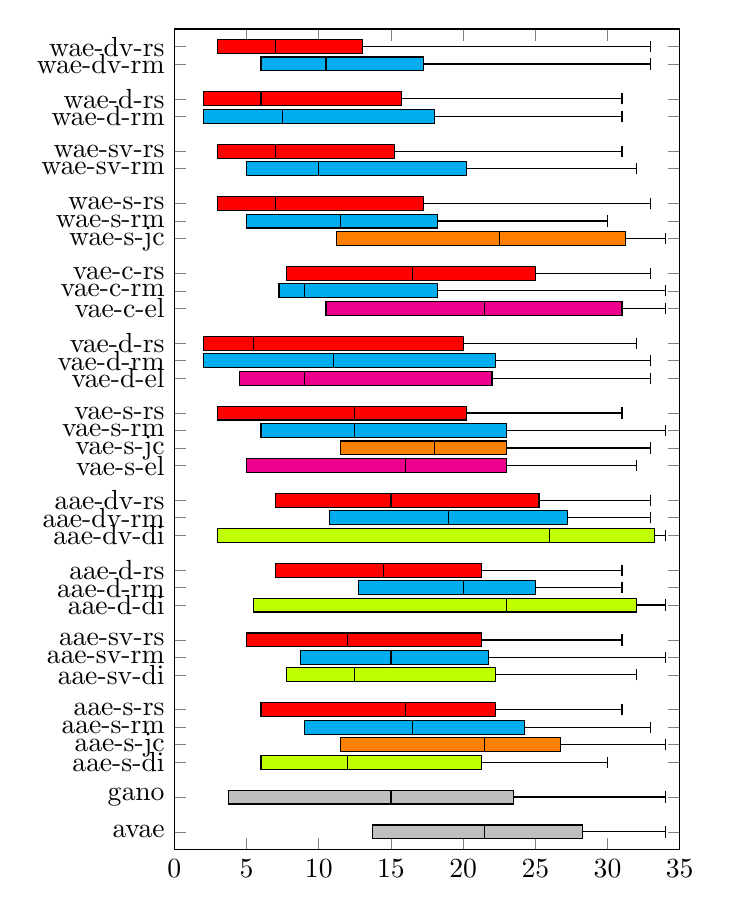
\begin{tikzpicture}
\begin{axis}[
	height=12cm,
	width=8cm,
	ymin=0, ymax=47,
	xmin=0, xmax=35,
	ytick={1,3,5,6,7,8,10,11,12,14,15,16,18,19,20,22,23,24,25,27,28,29,31,32,33,35,36,37,39,40,42,43,45,46},
	yticklabels={avae,gano,aae-s-di,aae-s-jc,aae-s-rm,aae-s-rs,aae-sv-di,aae-sv-rm,aae-sv-rs,aae-d-di,aae-d-rm,aae-d-rs,aae-dv-di,aae-dv-rm,aae-dv-rs,vae-s-el,vae-s-jc,vae-s-rm,vae-s-rs,vae-d-el,vae-d-rm,vae-d-rs,vae-c-el,vae-c-rm,vae-c-rs,wae-s-jc,wae-s-rm,wae-s-rs,wae-sv-rm,wae-sv-rs,wae-d-rm,wae-d-rs,wae-dv-rm,wae-dv-rs}
	]
\addplot [fill=lightgray, boxplot prepared={
draw position=1,
lower whisker=34, lower quartile=13.75,
median=21.5, upper quartile=28.25,
upper whisker=34},
] coordinates {};
\addplot [fill=lightgray, boxplot prepared={
draw position=3,
lower whisker=34, lower quartile=3.75,
median=15.0, upper quartile=23.5,
upper whisker=34},
] coordinates {};
\addplot [fill=lime, boxplot prepared={
draw position=5,
lower whisker=30, lower quartile=6.0,
median=12.0, upper quartile=21.25,
upper whisker=30},
] coordinates {};
\addplot [fill=orange, boxplot prepared={
draw position=6,
lower whisker=34, lower quartile=11.5,
median=21.5, upper quartile=26.75,
upper whisker=34},
] coordinates {};
\addplot [fill=cyan, boxplot prepared={
draw position=7,
lower whisker=33, lower quartile=9.0,
median=16.5, upper quartile=24.25,
upper whisker=33},
] coordinates {};
\addplot [fill=red, boxplot prepared={
draw position=8,
lower whisker=31, lower quartile=6.0,
median=16.0, upper quartile=22.25,
upper whisker=31},
] coordinates {};
\addplot [fill=lime, boxplot prepared={
draw position=10,
lower whisker=32, lower quartile=7.75,
median=12.5, upper quartile=22.25,
upper whisker=32},
] coordinates {};
\addplot [fill=cyan, boxplot prepared={
draw position=11,
lower whisker=34, lower quartile=8.75,
median=15.0, upper quartile=21.75,
upper whisker=34},
] coordinates {};
\addplot [fill=red, boxplot prepared={
draw position=12,
lower whisker=31, lower quartile=5.0,
median=12.0, upper quartile=21.25,
upper whisker=31},
] coordinates {};
\addplot [fill=lime, boxplot prepared={
draw position=14,
lower whisker=34, lower quartile=5.5,
median=23.0, upper quartile=32.0,
upper whisker=34},
] coordinates {};
\addplot [fill=cyan, boxplot prepared={
draw position=15,
lower whisker=31, lower quartile=12.75,
median=20.0, upper quartile=25.0,
upper whisker=31},
] coordinates {};
\addplot [fill=red, boxplot prepared={
draw position=16,
lower whisker=31, lower quartile=7.0,
median=14.5, upper quartile=21.25,
upper whisker=31},
] coordinates {};
\addplot [fill=lime, boxplot prepared={
draw position=18,
lower whisker=34, lower quartile=3.0,
median=26.0, upper quartile=33.25,
upper whisker=34},
] coordinates {};
\addplot [fill=cyan, boxplot prepared={
draw position=19,
lower whisker=33, lower quartile=10.75,
median=19.0, upper quartile=27.25,
upper whisker=33},
] coordinates {};
\addplot [fill=red, boxplot prepared={
draw position=20,
lower whisker=33, lower quartile=7.0,
median=15.0, upper quartile=25.25,
upper whisker=33},
] coordinates {};
\addplot [fill=magenta, boxplot prepared={
draw position=22,
lower whisker=32, lower quartile=5.0,
median=16.0, upper quartile=23.0,
upper whisker=32},
] coordinates {};
\addplot [fill=orange, boxplot prepared={
draw position=23,
lower whisker=33, lower quartile=11.5,
median=18.0, upper quartile=23.0,
upper whisker=33},
] coordinates {};
\addplot [fill=cyan, boxplot prepared={
draw position=24,
lower whisker=34, lower quartile=6.0,
median=12.5, upper quartile=23.0,
upper whisker=34},
] coordinates {};
\addplot [fill=red, boxplot prepared={
draw position=25,
lower whisker=31, lower quartile=3.0,
median=12.5, upper quartile=20.25,
upper whisker=31},
] coordinates {};
\addplot [fill=magenta, boxplot prepared={
draw position=27,
lower whisker=33, lower quartile=4.5,
median=9.0, upper quartile=22.0,
upper whisker=33},
] coordinates {};
\addplot [fill=cyan, boxplot prepared={
draw position=28,
lower whisker=33, lower quartile=2.0,
median=11.0, upper quartile=22.25,
upper whisker=33},
] coordinates {};
\addplot [fill=red, boxplot prepared={
draw position=29,
lower whisker=32, lower quartile=2.0,
median=5.5, upper quartile=20.0,
upper whisker=32},
] coordinates {};
\addplot [fill=magenta, boxplot prepared={
draw position=31,
lower whisker=34, lower quartile=10.5,
median=21.5, upper quartile=31.0,
upper whisker=34},
] coordinates {};
\addplot [fill=cyan, boxplot prepared={
draw position=32,
lower whisker=34, lower quartile=7.25,
median=9.0, upper quartile=18.25,
upper whisker=34},
] coordinates {};
\addplot [fill=red, boxplot prepared={
draw position=33,
lower whisker=33, lower quartile=7.75,
median=16.5, upper quartile=25.0,
upper whisker=33},
] coordinates {};
\addplot [fill=orange, boxplot prepared={
draw position=35,
lower whisker=34, lower quartile=11.25,
median=22.5, upper quartile=31.25,
upper whisker=34},
] coordinates {};
\addplot [fill=cyan, boxplot prepared={
draw position=36,
lower whisker=30, lower quartile=5.0,
median=11.5, upper quartile=18.25,
upper whisker=30},
] coordinates {};
\addplot [fill=red, boxplot prepared={
draw position=37,
lower whisker=33, lower quartile=3.0,
median=7.0, upper quartile=17.25,
upper whisker=33},
] coordinates {};
\addplot [fill=cyan, boxplot prepared={
draw position=39,
lower whisker=32, lower quartile=5.0,
median=10.0, upper quartile=20.25,
upper whisker=32},
] coordinates {};
\addplot [fill=red, boxplot prepared={
draw position=40,
lower whisker=31, lower quartile=3.0,
median=7.0, upper quartile=15.25,
upper whisker=31},
] coordinates {};
\addplot [fill=cyan, boxplot prepared={
draw position=42,
lower whisker=31, lower quartile=2.0,
median=7.5, upper quartile=18.0,
upper whisker=31},
] coordinates {};
\addplot [fill=red, boxplot prepared={
draw position=43,
lower whisker=31, lower quartile=2.0,
median=6.0, upper quartile=15.75,
upper whisker=31},
] coordinates {};
\addplot [fill=cyan, boxplot prepared={
draw position=45,
lower whisker=33, lower quartile=6.0,
median=10.5, upper quartile=17.25,
upper whisker=33},
] coordinates {};
\addplot [fill=red, boxplot prepared={
draw position=46,
lower whisker=33, lower quartile=3.0,
median=7.0, upper quartile=13.0,
upper whisker=33},
] coordinates {};
\end{axis}
\end{tikzpicture}

    \caption{Sensitivity study of various variants of  autoencoder-based methods displayed in the form of boxplots of their ranks in the AUC metric achieved on the tabular datasets. The first three letters of the method's name denote the training loss. Models with the -d- middle part estimate full diagonal of the decoder variance, -s- estimate only a scalar, and -c-  use a fixed scalar variance as a hyperparameter. All variants are using the standard Gaussian latent model. Models using the VampPrior are denoted by extending the decoder variance symbol by the letter v-, i.e. -dv-, -sv-, -cv-. The last part of the name denotes score, -rs stands for the sampled rec. probability~\eqref{eq:score_sample} with $L=100$, -rm for~\eqref{eq:score_mean}, -el for the ELBO~\eqref{eq:vae_loss} composed of -rs and KLD, -jc for~\eqref{eq:jacodeco}, -di for~\eqref{eq:disc_score}.}
    \label{fig:tabular_ae_only_box_auc_meanmax}
\end{figure}


\begin{table}
    \footnotesize
    \centering
    \tabcolsep=0.05cm
    \begin{tabular}{c|c c c c c}
         & vae-s-rs & vae-d-rs & vae-s-rm & vae-d-rm & vae-d-jc \\
         \midrule
        $\bar{t}_{pred}$ [s] & 12.10 & 18.51 & 0.11 & 0.15 & 57.31
    \end{tabular}
    \vspace*{0.15cm}
    \caption{Average prediction times on the  tabular datasets for different combinations of VAE scores and decoder variance estimations. The -d- part stands for model with an estimate of the full diagonal of the decoder variance, -s- is a scalar estimate. Sampled reconstruction error~\eqref{eq:score_sample} is denoted as -rs, -rm is the anomaly score~\eqref{eq:score_mean} and -jc is~\eqref{eq:jacodeco}.}
    \label{tab:predict_times}
\end{table}



\subsubsection{Sensitivity study of OC-SVM}
\label{sub:OC-SVM}
The domination of OC-SVM on tabular data in anomaly validation context contrasts to many prior experimental comparisons~\cite{goldstein2016comparative, chalapathyGroupAnomalyDetection2018, deecke2018image, gopalanPIDForestAnomalyDetection2019, iwataSupervisedAnomalyDetection2019, wang2020advae}. The search for the culprit found it to be the hyperparameter selection. This study has varied the $\nu$ parameter, kernels, and their parameters, which is much more than the most prior art does, which is fixing the kernel to RBF and tests few values of its width $\gamma$ and $\nu.$ Inclusion of other kernels into the search for hyperparameters seems to be the major source of improvement in this case. Replacing the OC-SVM with one restricted to use only the RBF kernel and $\nu=0.5$ yields an increase in average rank from $2.9$ to $8.1$ with an average decrease in performance by $0.06$, measured in AUC in the anomaly validation context. This version of OC-SVM is then easily surpassed by variational autoencoders and kNN, as demonstrated in Supplementary, Tab.~\ref{tab:tabular_auc_auc_meanmax_orbf_ranks_only}.  The importance of the choice of the kernel is furthermore illustrated by the fact that the sigmoid kernel was the optimal choice for 23 datasets, while the RBF kernel was optimal only for 13. Ref.~\cite{goldstein2016comparative} mentions that setting $\nu=0.5$ provides universally good results, which may be the reason why many authors do not tune it. In theory, it should be set to much lower values ($\nu = 0.05$) corresponding to the presumed low ratio of anomalies in data, but with Bayesian optimization, we found that the best estimate of $\nu$ was in some cases even higher, such as $\sim0.75$ on the statlog-vehicle dataset.

\subsection{Economic context}
\label{sec:economic_context}
\begin{figure*}
    \centering
    \begin{subfigure}{\columnwidth}
        \centering
        \small
        \resizebox {\linewidth}{!}{
            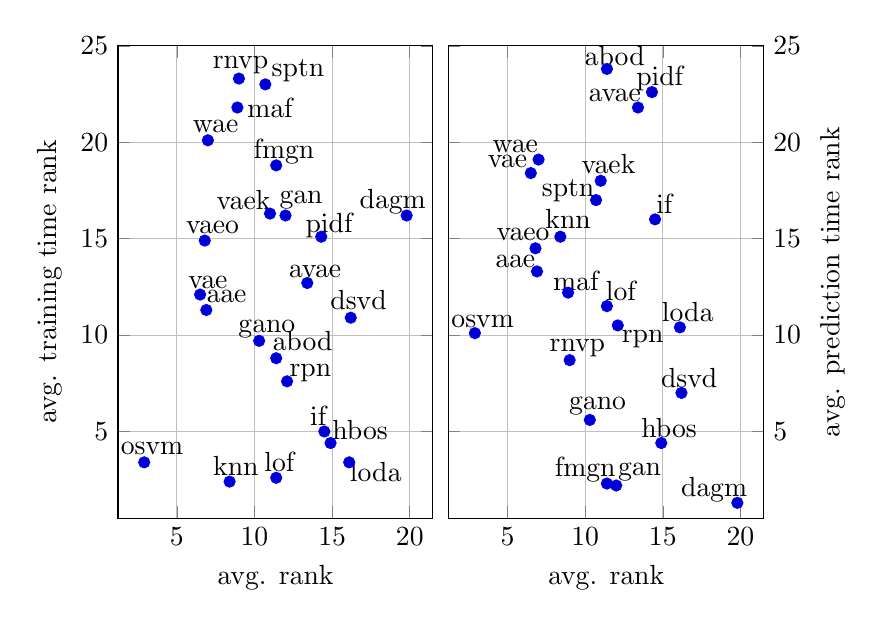
\begin{tikzpicture}[]
\begin{groupplot}[group style={vertical sep = 0.0cm, horizontal sep = 0.2cm, group size=2 by 1}]

\nextgroupplot [
  xlabel = {avg. rank},
  ylabel = {avg. training time rank},
  ylabel near ticks, yticklabel pos=left,
  ymin = 0.5, ymax=25,
  width=4cm, height=6cm, scale only axis=true,
  grid=major,
  % title = {(fit time)}
]

\addplot+[
  draw = none
] coordinates {
  (6.9, 11.3)
  (11.4, 8.8)
  (13.4, 12.7)
  (19.8, 16.2)
  (16.2, 10.9)
  (11.4, 18.8)
  (12.0, 16.2)
  (10.3, 9.7)
  (14.9, 4.4)
  (14.5, 5.0)
  (8.4, 2.4)
  (16.1, 3.4)
  (11.4, 2.6)
  (8.9, 21.8)
  % (22.3, 19.4)
  (2.9, 3.4)
  (14.3, 15.1)
  (9.0, 23.3)
  (12.1, 7.6)
  (10.7, 23.0)
  (6.5, 12.1)
  (11.0, 16.3)
  (6.8, 14.9)
  (7.0, 20.1)
};

\node at (axis cs:8.2, 12.0) {aae};

\node at (axis cs:13.1, 9.7) {abod};

\node at (axis cs:13.9, 13.3) {avae};

\node at (axis cs:18.9, 16.9) {dagm};

\node at (axis cs:16.7, 11.8) {dsvd};

\node at (axis cs:11.9, 19.5) {fmgn};

\node at (axis cs:13.0, 17.0) {gan};

\node at (axis cs:10.8, 10.3) {gano};

\node at (axis cs:16.8, 5.1) {hbos};

\node at (axis cs:14.1, 5.8) {if};

\node at (axis cs:8.8, 3.2) {knn};

\node at (axis cs:17.8, 2.9) {loda};

\node at (axis cs:11.6, 3.4) {lof};

\node at (axis cs:11.0, 21.8) {maf};

% \node at (axis cs:22.8, 20.0) {mgal};

\node at (axis cs:3.4, 4.1) {osvm};

\node at (axis cs:14.8, 15.7) {pidf};

\node at (axis cs:9.1, 24.0) {rnvp};

\node at (axis cs:13.6, 8.0) {rpn};

\node at (axis cs:12.8, 23.7) {sptn};

\node at (axis cs:7.0, 12.7) {vae};

\node at (axis cs:9.3, 17.0) {vaek};

\node at (axis cs:7.3, 15.6) {vaeo};

\node at (axis cs:7.5, 20.8) {wae};

\nextgroupplot [
  xlabel = {avg. rank},
  ylabel = {avg. prediction time rank},
  ylabel near ticks, yticklabel pos=right,
  ymin = 0.5, ymax=25,
  width=4cm, height=6cm, scale only axis=true,
  % title = {(evaluation time)},
  grid=major,
  % yticklabels={}
]

\addplot+[
  draw = none
] coordinates {
  (6.9, 13.3)    
  (11.4, 23.8)    
  (13.4, 21.8)
  (19.8, 1.3)
  (16.2, 7.0)
  (11.4, 2.3)
  (12.0, 2.2)
  (10.3, 5.6)
  (14.9, 4.4)
  (14.5, 16.0)
  (8.4, 15.1)
  (16.1, 10.4)
  (11.4, 11.5)
  (8.9, 12.2)
  % (22.3, 10.0)
  (2.9, 10.1)
  (14.3, 22.6)
  (9.0, 8.7)
  (12.1, 10.5)
  (10.7, 17.0)
  (6.5, 18.4)
  (11.0, 18.0)
  (6.8, 14.5)
  (7.0, 19.1)
};

\node at (axis cs:5.5, 13.8) {aae};

\node at (axis cs:11.9, 24.5) {abod};

\node at (axis cs:11.9, 22.4) {avae};

\node at (axis cs:18.3, 2.0) {dagm};

\node at (axis cs:16.7, 7.8) {dsvd};

\node at (axis cs:10.0, 3.0) {fmgn};

\node at (axis cs:13.5, 2.9) {gan};

\node at (axis cs:10.8, 6.3) {gano};

\node at (axis cs:15.4, 5.2) {hbos};

\node at (axis cs:15.1, 16.8) {if};

\node at (axis cs:8.9, 16.0) {knn};

\node at (axis cs:16.6, 11.2) {loda};

\node at (axis cs:12.3, 12.3) {lof};

\node at (axis cs:9.4, 12.8) {maf};

% \node at (axis cs:22.8, 10.7) {mgal};

\node at (axis cs:3.4, 10.7) {osvm};

\node at (axis cs:14.8, 23.3) {pidf};

\node at (axis cs:9.5, 9.3) {rnvp};

\node at (axis cs:13.7, 9.8) {rpn};

\node at (axis cs:8.9, 17.5) {sptn};

\node at (axis cs:5.0, 19.0) {vae};

\node at (axis cs:11.5, 18.9) {vaek};

\node at (axis cs:6.0, 15.2) {vaeo};

\node at (axis cs:5.5, 19.8) {wae};

\end{groupplot}
\end{tikzpicture}


        }
        \caption{tabular datasets}
        \label{fig:tabular_total_eval_t_fit_t_combined}
    \end{subfigure}
    \begin{subfigure}{\columnwidth}
        \centering
        \small
        \resizebox {\linewidth}{!}{
            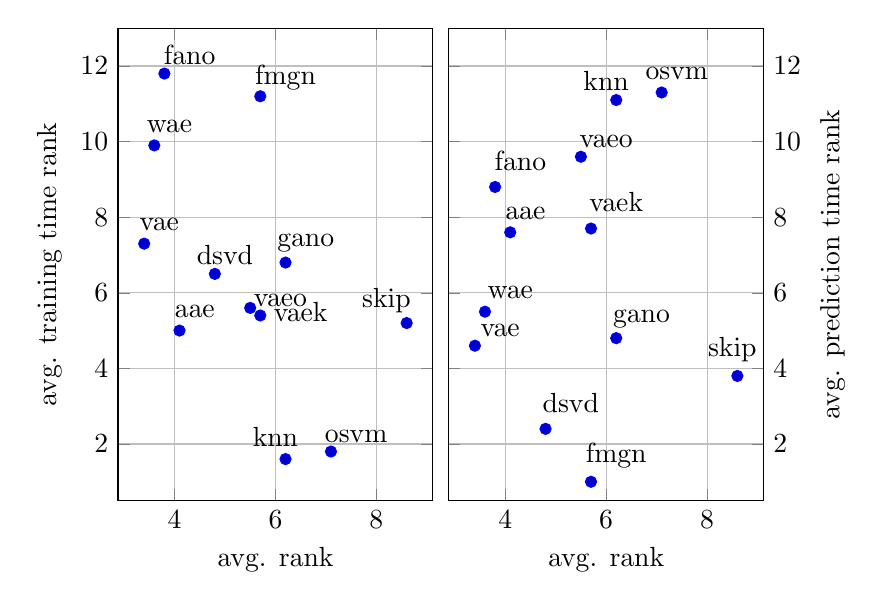
\begin{tikzpicture}[]
\begin{groupplot}[group style={vertical sep = 0.0cm, horizontal sep = 0.2cm, group size=2 by 1}]

\nextgroupplot [
  xlabel = {avg. rank},
  ylabel = {avg. training time rank},
  ylabel near ticks, yticklabel pos=left,
  ymin = 0.5, ymax=13,
  width=4cm, height=6cm, scale only axis=true,
  grid=major,
  % title = {(fit time)}
]

\addplot+[
  draw = none
] coordinates {
  (4.1, 5.0)
  (4.8, 6.5)
  (3.8, 11.8)
  (5.7, 11.2)
  (6.2, 6.8)
  (6.2, 1.6)
  (7.1, 1.8)
  (8.6, 5.2)
  (3.4, 7.3)
  (5.7, 5.4)
  (5.5, 5.6)
  (3.6, 9.9)
};

\node at (axis cs:4.4, 5.5) {aae};

\node at (axis cs:5.0, 7.0) {dsvd};

\node at (axis cs:4.3, 12.3) {fano};

\node at (axis cs:6.2, 11.7) {fmgn};

\node at (axis cs:6.6, 7.3) {gano};

\node at (axis cs:6.0, 2.2) {knn};

\node at (axis cs:7.6, 2.2) {osvm};

\node at (axis cs:8.2, 5.8) {skip};

\node at (axis cs:3.7, 7.8) {vae};

\node at (axis cs:6.5, 5.5) {vaek};

\node at (axis cs:6.1, 5.8) {vaeo};

\node at (axis cs:3.9, 10.4) {wae};

\nextgroupplot [
  xlabel = {avg. rank},
  ylabel = {avg. prediction time rank},
  ylabel near ticks, yticklabel pos=right,
  ymin = 0.5, ymax=13,
  width=4cm, height=6cm, scale only axis=true,
  % title = {(evaluation time)},
  grid=major,
  % yticklabels={}
]

\addplot+[
  draw = none
] coordinates {
  (4.1, 7.6)
  (4.8, 2.4)
  (3.8, 8.8)
  (5.7, 1.0)
  (6.2, 4.8)
  (6.2, 11.1)
  (7.1, 11.3)
  (8.6, 3.8)
  (3.4, 4.6)
  (5.7, 7.7)
  (5.5, 9.6)
  (3.6, 5.5)
};

\node at (axis cs:4.4, 8.1) {aae};

\node at (axis cs:5.3, 3.1) {dsvd};

\node at (axis cs:4.3, 9.5) {fano};

\node at (axis cs:6.2, 1.7) {fmgn};

\node at (axis cs:6.7, 5.3) {gano};

\node at (axis cs:6.0, 11.6) {knn};

\node at (axis cs:7.4, 11.8) {osvm};

\node at (axis cs:8.5, 4.5) {skip};

\node at (axis cs:3.9, 5.0) {vae};

\node at (axis cs:6.2, 8.4) {vaek};

\node at (axis cs:6.0, 10.0) {vaeo};

\node at (axis cs:4.1, 6.0) {wae};

\end{groupplot}
\end{tikzpicture}


        }
        \caption{image datasets}
        \label{fig:images_total_eval_t_fit_t_combined}
    \end{subfigure}
    \caption{Scatter-plots of the average rank in the AUC metric on the tabular  (a) and image (b) data versus average rank of the computational complexity of the displayed methods measured via training time (left) and prediction time (right). MO-GAAL has been omitted from the tabular figures, as its performance positioned it too far to the right with the training time rank of $19.4$ and the prediction time rank of $10.0$.}
    \label{fig:images_total_eval_t_fit_t_combined_joined}
\end{figure*}

Practitioners ask for fast and accurate algorithms, but these two features rarely go hand in hand, and a decision on a trade-off has to be made. Interesting methods lie on the Pareto frontier, as in the absence of an external factor, rationally behaving practitioner does not have a motivation to choose a different model.

Fig.~\ref{fig:tabular_total_eval_t_fit_t_combined}-left shows the trade-off between accuracy and training time for tabular data, where the absolute numbers were replaced by average ranks for robustness. The Pareto frontier contains two methods, which are OC-SVM and kNN. The position of OC-SVM is rather surprising, as its training time is known to scale poorly (quadratically) with respect to the number of samples, but it is caused by most of the tabular datasets being small. Different results may arise for a dataset with many data records. Fig.~\ref{fig:tabular_total_eval_t_fit_t_combined}-right shows a similar trade-off between accuracy and testing (inference) time. OC-SVM is still on the Pareto frontier, but it is expensive, as the complexity grows linearly in the number of samples. fmGAN, GAN and DAGMM methods are there as well -- these methods have fast inference but lower accuracy.

We provide results averaged over the studied contexts on image data. Due to the variability of the results in each context, the x-axis will vary. In the averaged ranks, VAE is on the Pareto front in both fit and prediction times, see Fig.~\ref{fig:images_total_eval_t_fit_t_combined}. Its prediction complexity is given mainly by choice of the number of samples taken in the computation of the sampled reconstruction score~\eqref{eq:score_sample}. The kNN detector has negligible training time, given only by the construction of the tree structure representing data, but seems to be mostly unusable on image data due to slow prediction times on datasets that are large in dimension and number of samples. The fmGAN finds itself in a completely reversed scenario.

\subsection{Other influences}
\label{sec:other_context}
In this section, we report the results of three sources of variability of performance of AD methods that were found to have minimal impact.

\emph{Ensembles/Hyperparameter averaging} The benefits of ensembles in prior art seem to be mixed. While~\cite{choiWAICWhyGenerative2019} claims that a combination of VAE or GAN ensembles using WAIC might be useful, Ref.~\cite{nalisnickDeepGenerativeModels2019} claims a negligible effect. In our experiments, we have used ensembles as a way to reduce uncertainty in hyperparameters~\cite{wilson2020case}, meaning that unlike in~\cite{choiWAICWhyGenerative2019}, models in ensembles were of a single type differing only in architecture. The effect of such an ensemble on average AUC was overall zero, sometimes even negative, see Supplementary~\ref{sec:appendix_ensembles}, Tab.~\ref{tab:ensembles_sensitivity_grouped}. Exceptions are methods based on GANs featuring improvements by $0.02$ in average AUC. These findings are on par with those in~\cite{nalisnickDeepGenerativeModels2019}.

\emph{Bayesian optimization} Bayesian optimization was introduced as an alternative to a random search of hyperparameters. It has the potential to find better hyperparameters with a low number of trials. Comparison of the random search and Bayesian optimization under the same conditions is reported in the Supplementary, Tab.~\ref{tab:tabular_bayes_comparison}. We can conclude that Bayesian optimization was able to find hyperparameters with better performance for the vast majority of the methods. However, this improvement is often quite small and insufficient to change the ranks of the methods. Notable exceptions are the GANomaly and GAN methods which improved by two ranks. 

\emph{Performance metric AUC/TPR} The hypothesis that the methods may perform differently when chosen for different optimization criteria than the usual AUC has not been proved. The results are summarized in the Supplementary, Tab.~\ref{tab:metric_comparison_grouped}. While small changes in performance have been observed, the ranks of the methods remain the same in both criteria, AUC and TPR@5\%. 

\section{Conclusion}
The presented extensive comparison of anomaly detection methods based on deep generative methods, namely variants of flows, variational autoencoders, and generative adversarial networks with methods based on alternative paradigms (Support vector machines, random forests, histogram, and distance-based methods) revealed that the performance of anomaly detection methods strongly depends on experimental conditions. We have identified the main sources of variation to be the choice of data and hyperparameter tuning. We presented detailed results under a combination of experimental conditions, called contexts, specifically the data context, hyperparameter context, and economic context. 

In the dataset context, a clear distinction in performance was found between tabular data, image data containing statistical and semantic anomalies. The main distinction in hyperparameter selection was how many anomalies were present in the validation set. Different order of performance of the tested method was observed for a different combination of dataset type and hyperparameter selection context, explaining various outcomes of comparison in the prior art. We strongly recommend that authors provide more details on the context of their experimental studies in the future.

The comparison is not only aimed at researchers but also at practitioners desiring accurate methods with low computational complexity. Therefore, we visualize these trade-offs between performance and computational cost. Also, we present a list of some of the most important practical observations and recommendations.
\begin{itemize}
    \item Methods with more exact likelihood modeling, such as kNN, flow, and autoencoder-based models, perform better in scenarios with a limited number of anomalies available for hyperparameter tuning.
    \item Majority of the methods fail to detect semantic anomalies. The exception is the fmGAN, but only if given enough computational resources and many anomalous samples for cross-validation. 
    \item OC-SVM, when properly tuned, can defeat most of the state-of-the-art on tabular data, although it suffers from overfitting when hyperparameters are selected using too few anomalies in the validation set.
    \item The method of the first choice appears to be the VAE/WAE due to its relatively cheap, precise, and consistent performance in most of the experiments. However, it possesses so many degrees of freedom that it forms a full family of methods. It was found that the best performance is obtained when estimating the full variance of samples on the output of the decoder and evaluating anomalies using sampled reconstruction score. 
\end{itemize}

Many aspects have not been covered and remain a topic of future work, such as the identification of the relevant kind of anomalies in the semantic datasets or the design of ensembles of methods of various types. Although we have shown that the number of anomalies available for validation is an important context, there was no further budget for a comparison of anomaly detection methods with active learning.  We have also completely left out the comparison of models on temporal data, such as time series or video, which is a very challenging task. Finally, an interesting area to study further is the influence of the presence of unlabeled anomalies in the training data.


\chapter{Anomaly detection in multi-factor data} \label{sec:chapter_sgvaegan}

\section{Introduction}

In the course of this text, we have been gathering information about state-of-the-art methods, available datasets, and potential unsolved problems in anomaly detection. The ultimate goal of this endeavour was to find an intriguing anomaly detection problem and propose a novel method for its solution, which will be presented in this chapter. Here is a list of the findings that have been gathered so far.

\begin{enumerate}
    \item In Section~\ref{sec:alfven}, the problem of identifying anomalies in high-resolution image data was solved and the two-stage model approach proved to be the most successful. The best models were a combination of a probabilistic autoencoder, which produced informative latent encoding, and a classical anomaly detector, which operated on the encoded data of highly reduced dimensionality. The dimensionality reduction alleviated the computational burden from the second stage model which could be more deeply fine-tuned. Eventually, a simple kNN detector was the best choice for a second-stage model. 
    \item In Chapter~\ref{sec:chapter_comparison}, a thorough comparison of existing anomaly detectors was done. We have seen what are the most important contexts of an anomaly detection problem (data type, number of labeled anomalies, and budget available for hyperparameter tuning) that one should consider when choosing a method for solving a practical problem. It was shown that deep generative models gain an edge over other methods when solving anomaly detection problems on image data, especially on problems where semantic anomalies occur. 
    \item In the same chapter, it was shown that although probabilistic autoencoders are generally well-suited for image anomaly detection problems, adversarial training might be beneficial for the detection of \textbf{semantic} anomalies~\cite{ahmed2020detecting} with enough budget for hyperparameter tuning. In fact, the majority of the methods compared in Chapter~\ref{sec:chapter_comparison} failed in the detection of semantic anomalies.
\end{enumerate}

Since the detection of semantic anomalies in images is a relatively novel field, we have decided to cover this problem in this chapter using the findings described in the list above. Semantic anomalies appear most often in visual data and their anomality is based on the high-level (semantic) information in the image. For example, an image (used in~\cite{vskvara2021comparison}) can be anomalous because it is blurred, or because it has a different object in the foreground (e.g. plane in the sky instead of a bird in the sky), or different background (e.g. the plane is on a runway, whereas it is usually on the sky). From the point of view of the above definition, they are all anomalies, but the user might be interested in anomalies of a certain type, or they might want the anomalies to be automatically classified according to their type. This difference can only be made based on the high-level, semantic information of an image. A good semantic detector should be also robust to non-semantic shifts~\cite{ahmed2021systematic}, i.e. data-generating factors that are not present in the training data but are not considered anomalous. The detection of semantic anomalies has been previously studied under the name \textbf{subspace} anomaly detection~\cite{raz2002semantic, kriegel2009outlier,rahmani2016randomized}. The idea, as the name suggests, is that the anomaly is not visible in the full input space, where it might be shadowed by noise, but only in the subspace. The subspace is most of the time "axis parallel" or defined in a linear transformation of the input space. Semantic anomalies further generalize this to non-linear transformations.

It seems unlikely in practice that the subspace in which anomalies would be detectable would be aligned with the input space, or with its linear transformation. Contrary, independent components emerge after non-linear projections as shown in~\cite{burgess2018understanding, kim2018disentangling, esmaeili2019structuredhfvae, tschannen2018recent, bai2021contrastively, kim2019bayes, deecke2021transfer}, which motivates this work. Here, we propose to disentangle the input into independent factors, each providing an anomaly score. Ideally, a semantic anomaly and its source would be then better detectable by one of these scores rather than by a score given to the original input. 

In this chapter, the proposed disentanglement into independent factors and the resulting composition of anomaly scores is first theoretically justified. This multi-factor anomaly score is a weighted combination of anomaly scores corresponding to individual factors of the disentangled latent space. In Sec.~\ref{sec:model}, the concrete details (construction, training, and evaluation) of the novel model are described. In the experimental Sec.~\ref{sec:experiments}, the proposed model is extensively compared to baselines on several image benchmarks. It is demonstrated that the model is capable of detecting the factor that is the most likely source of the anomaly in the unsupervised case, and quickly improves with very few labeled samples.

\section{Decomposing the anomaly score} 
\label{sec:theory}
In this section, we will derive a general formula for the computation of the anomaly score of a VAE model for the case when the latent space can be disentangled into independent components. This will be useful as a theoretical foundation of the proposed anomaly detector in Sec.~\ref{sec:model}.

\subsection{Orthogonal generative model} \label{sec:orthogonal_score}
Let us remind ourselves that the VAE (see Sec.~\ref{sec:vanilla_vae}) fits a generative model with data $\vc{x} \in \mathbb{R}^d$
\begin{align}
p_{\vc{\theta}}(\vc{x}) & = \int_{\mathcal{Z}} p_{\vc{\theta}}(\vc{x} \vert \vc{z})p(\vc{z})d\vc{z} & p_{\vc{\theta}}(\vc{x} \vert \vc{z}) & =\mathcal{N}(\vc{x};\vc{\mu}_{\vc{\theta}}(\vc{z}),\vc{\sigma}^{2} \mathbf{I}),\label{eq:vae}
\end{align}
where $p_{\vc{\theta}}(\vc{x}\vert \vc{z})$ is the decoder and the prior on the latent $h$-dimensional variable $z$ is either fixed $p(\vc{z})=\mathcal{N}(0,\mathbf{I})$, or further parametrized $p_{\vc{\theta}}(\vc{z})$, e.g. as in~\cite{tomczak2017vae}. The VAE also includes an encoder $q_{\vc{\phi}}(\vc{z}\vert \vc{x})$ and is optimized by minimization of the ELBO objective~\eqref{eq:elbo3}. 

The above generative model~\eqref{eq:vae} can be rewritten as $\vc{x}=\vc{\mu}_{\vc{\theta}}(\vc{z})+\vc{e}$ where $\vc{e}$ is (usually isotropic) Gaussian noise. This formulation emphasizes the need for marginalization since $\vc{\mu}_{\vc{\theta}}(\vc{z})$ is a random variable of dimension $h$ (same as that of the latent space $\mathcal{Z}$) and noise $\vc{e}$ is a random variable of dimension $d,$ which is the same as the data. Equation~\eqref{eq:vae} therefore marginalizes away random variables corresponding to latent $z.$ Due to this ambiguity, the assignment between $x$ and $z$ is not unique. In fact, for any $\vc{x}$ exists  $\vc{z}'$~\cite{pidhorskyi2018generative, vsmidl2019anomaly} such that \[
\vc{x}=\vc{x}' + +\vc{e}^{\bot} = \vc{\mu}_{\vc{\theta}}(\vc{z}')+\vc{e}^{\bot}
\]
where $\vc{e}^{\bot}$ is the observation noise that lies in the normal space perpendicular to the manifold defined by the decoder mean $\vc{\mu}_{\vc{\theta}}(\vc{z})$. This interpretation implies independence between $\vc{\mu}_{\vc{\theta}}(\vc{z}')$ and $\vc{e}^\bot$, which allows for the approximation 
\begin{equation}
p_{\vc{\theta}}(\vc{x})\approx p(\vc{\mu}_{\vc{\theta}}(\vc{z}'))p(\vc{e}^{\bot}). 
\end{equation}

However, the independence relation was found~\cite{vsmidl2019anomaly} to be sufficiently accurate even for the original noise estimate, $\vc{x}=\vc{x}'+\vc{e}$.  The  probability of the reconstruction $p_{\vc{\theta}}(\vc{x}')$ is given by the change of coordinate formula from $p_{z}(\vc{z})$ (here we use the subscript $_z$ in order to distinguish that the distribution is on the latent space $\mathcal{Z}$), yielding
\begin{align}
p_{\vc{\theta}}(\vc{x})\approx p_{\vc{\theta}}(\vc{x}')p(\vc{e})=p_{z}(\vc{\mu}_{\vc{\theta}}^{-1}(\vc{x}'))\left\vert \frac{\partial \vc{\mu}_{\vc{\theta}}^{-1}(\vc{x})}{\partial \vc{x}}\right\vert p(\vc{e}).\label{eq:pxjacodeco}
\end{align}
A gaussian noise model might be assumed, e.g. $p(\vc{e}) = \mathcal{N}(\vc{x}-\vc{x}',\vc{\sigma}^{2}\mathbf{I})$. In practice, an anomaly score for the orthogonal model $s(\vc{x}) = - \log p_{\vc{\theta}}(\vc{x})$ is computed as
\begin{align}
s(\vc{x}) & = - \log p(\vc{e}) -\log p_{z}(\vc{z})-\log\left\vert \frac{\partial \vc{\mu}_{\vc{\theta}}^{-1}(\vc{x})}{\partial \vc{x}}\right\vert ,\label{eq:jacodeco}
\end{align}
which is essentially the reconstruction error with additional terms.

\subsection{Anomaly in the latent space}
Let's observe how the above generative model changes when we assume the distribution on latent $\vc{z}$ to be multi-modal conditioned by hidden label $y$. This simplification assumes that the latent distribution for normal and anomalous data is different. Let
\begin{equation} \label{eq:pzy}
p_z(\vc{z}\vert y)=p_{n}(\vc{z})^{y}p_{a}(\vc{z})^{1-y},y\in[0,1],
\end{equation}
where $y=1$ for normal data, $y=0$ for anomalies, and $p_n(\vc{z}),p_a(\vc{z})$ are the latent distributions of normal and anomalous data, respectively. Then from~\eqref{eq:jacodeco} we have
\begin{align*}
s(\vc{x} \vert y) & = - \log p(\vc{e}) -y\log p_{n}(\vc{z})  -(1-y)\log p_{a}(\vc{z}) - \log\left\vert \frac{\partial \vc{\mu}_{\vc{\theta}}^{-1}(\vc{x})}{\partial \vc{x}}\right\vert,
\end{align*}
Since $y$ is usually unknown, we will integrate it away by expectation over $y$, 
\begin{align}
\mathbb{E}_{p(y)} \left[  s(\vc{x} \vert y) \right]  = &  - \log p(\vc{e}) - \log\left\vert \frac{\partial \vc{\mu}_{\vc{\theta}}^{-1}(\vc{x})}{\partial \vc{x}}\right\vert \nonumber \\ 
 & - \int_{\mathcal{Y}} y\log p_{n}(\vc{z}) p(y) dy - \int_{\mathcal{Y}} (1-y)\log p_{a}(\vc{z}) p(y) dy \nonumber \\
   \propto & - \log p(\vc{e}) - \log\left\vert \frac{\partial \vc{\mu}_{\vc{\theta}}^{-1}(\vc{x})}{\partial \vc{x}}\right\vert  - \alpha\log p_{n}(\vc{z}) = s(\vc{x}). \label{eq:jacodeco2}
\end{align}
where we assume $\mathbb{E}_{p(y)} \left[  y \right] =\alpha$, and $p_{a}(\vc{z}) \propto 1$, because the probability of an anomaly is assumed to be the same everywhere, which then allows us to drop this term since it is independent of $\vc{x}$.  


Now consider a \textbf{disentagled} model, where the data is generated from multiple independent latent spaces, $\vc{z}=\vc{z}_{1},\ldots,\vc{z}_{l}$, 
\begin{equation} \label{eq:multilatent}
\vc{x}=f(\vc{z}_{1},\ldots,\vc{z}_{l})+\vc{e},
\end{equation}
where each of the latents has distribution $p(\vc{z}_{i})=\mathcal{N}(0,\mathbf{I})$. Using the same derivations, each of the latent spaces $\vc{z}_i$ can be a potential source of different types of anomalies, with hidden labels  $y=(y_{1},\ldots,y_{l})   $. Therefore, instead of~\eqref{eq:pzy},  we have
\begin{equation} 
p(\vc{z}\vert y)= \prod_{i=1}^l p_{n_i}(\vc{z}_i)^{y_i}p_{a_i}(\vc{z}_i)^{1-y_i},y_i\in[0,1].
\end{equation}
Repeating derivation of (\ref{eq:jacodeco2}) for multiple latent variables, the anomaly score becomes
\begin{align} \label{eq:alphadeco}
s(\vc{x}) & = - \log p(\vc{e}) - \log\left\vert \frac{\partial \vc{\mu}_{\vc{\theta}}^{-1}(\vc{x})}{\partial \vc{x}}\right\vert  -  \sum_{i=1}^{l}\alpha_{i}\log p_{n_{i}}(\vc{z}_{i}),
\end{align}
where $\alpha_{i}$ denotes the probability that the latent variable of the $i$th factor is generated from the normal class. In this work, we assume that $\alpha_i$ is not known during training but has to be estimated in the validation stage from examples of anomalous samples.\footnote{Based on the industrial experience of authors, this assumption is safe, i.e. there are usually examples of anomalies, though their diversity might be low.}

The interpretation of the values of $\alpha_i$ will be important later, in Sec.~\ref{sec:model}, where we construct the latent spaces to give them a specific meaning, and in Sec.~\ref{sec:anomaly_detection}, where we describe their fitting. Fitting the values of all $\alpha_i$ on a set of labeled data is equal to estimating the mean of $p(y_i)$ for the given data. This can be interpreted as estimating how likely it is for an anomaly to appear in the $i$-th latent in the context of the current dataset. 

In contrast, for a single data sample, we are more interested in the actual values of $y_i$, which are binary and which determine whether the sample is anomalous in the context of the latent space $i$. Their estimation is equal to the estimation of the distributions $p(y_i \vert \vc{x})$ and will be discussed in Sec.~\ref{sec:anomaly_factor_identification}. 

\section{Shape-guided decomposition} \label{sec:model}
\begin{figure}[ht!]
    \centering
    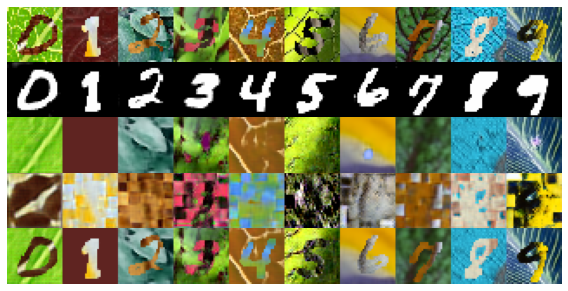
\includegraphics[width=\textwidth]{data/chapter_sgvaegan/fig1_wmnist_grid.png}
    \caption{Examples of decomposition on the Wildlife MNIST dataset by the SGVAEGAN model. The first row contains the input samples, below that are the decoded masks, backgrounds, foregrounds, and finally the whole reconstructions. The model can learn appropriate masks in an unsupervised fashion.}
    \label{fig:wmnist_grid}
\end{figure}

We demonstrate the advantage of disentanglement in detecting semantic anomalies on image data, because (i) the disentanglement has been researched mostly in this domain~\cite{kim2018disentangling, kim2019bayes, choi2020discond}, (ii) the anomaly detection community is the most active in this field, and (iii) the findings of Chapter~\ref{sec:chapter_comparison} showed that most deep generative models are not very efficient when dealing with semantic anomalies.

For the construction of the proposed model, we assume an image $\vc{x}$ to be composed of three main components: a mask (shape of the object), a background texture, and a foreground texture (the object). This of course is not true for all images, but many open datasets contain images that are structured this way. The mask together with the foreground texture defines the semantic meaning of the object, as it is what defines the class of the image in datasets. According to the above assumptions, each component (mask, background texture, and foreground texture) is generated from an independent variable. Therefore, for the latent distribution $p(\vc{z})$ it holds that
\begin{equation} \label{eq:latent_decomposition}
     p(\vc{z}) = p_{z_{m}}(\vc{z}_{m})p_{z_{f}}(\vc{z}_{f})p_{z_b}(\vc{z}_{b}),
\end{equation}
where subscripts $m,f,b$ denote the mask, foreground, and background latent variable, respectively. 
A representative example of a dataset where each image is composed of three independent components is the Wildlife MNIST dataset~\cite{sauer2021counterfactual}. It is constructed using masks from MNIST~\cite{lecun2010mnist} combined with foreground and background textures from~\cite{cimpoi2014describing} (see more details on its construction in Appendix~\ref{sec:appendix_datasets}). For examples from individual classes see the top row of Fig.~\ref{fig:wmnist_grid}. 

The independent decomposition~\eqref{eq:latent_decomposition} is akin to~\eqref{eq:multilatent}, but here we ascribe high-level semantic meaning to the individual latent spaces. This means that the model built on top of the assumption~\eqref{eq:latent_decomposition} has an inductive bias, which enables the unsupervised disentangled representation of the individual components of an image. The independency is further reinforced by the fact that the parts of the model responsible for the representation of the components do not share weights. Furthermore, since we want to apriori ascribe specific meaning to the disentangled latent spaces, we cannot use automatic disentanglement of individual dimensions as is the case in literature~\cite{burgess2018understanding, kim2019bayes, deecke2021transfer}, since there, the disentanglement is not unique and the semantic meaning of the disentangled factors has to be found manually in a post-processing phase.

In this section, the structure of the proposed generative model with independent latent spaces and its training procedure is described first. Then, in order to be able to detect and describe semantic anomalies, we combine the model with the anomaly score derived in Sec.~\ref{sec:theory}.

\subsection{Shape-guided VAEGAN model} \label{sec:sgvaegan}
 \begin{figure}[ht]
    \centering
       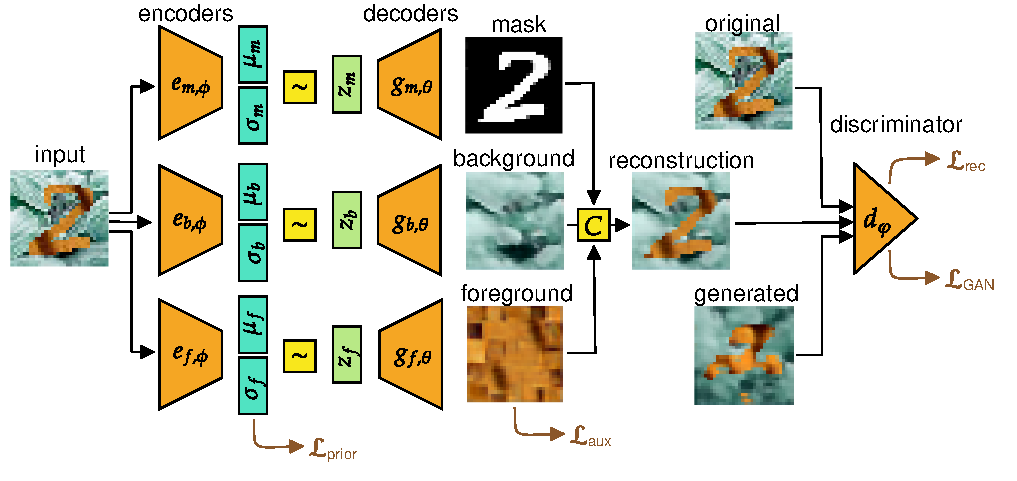
\includegraphics[width=\textwidth]{data/chapter_sgvaegan/fig2_sgvaegan_losses.pdf}
    \caption{The schema of the proposed model. Convolutional blocks are denoted in orange, fully connected in cyan, and intermediate representations in green. The yellow squares represent special operations - $c$ is the composition~\eqref{eq:composition} and the reparametrization trick is denoted by $\sim$. The generated sample is obtained by feeding samples from priors $\mathcal{N}(0,\mathbf{I})$ to the decoders.}
    \label{fig:sgvaegan_schema}
\end{figure}

The model disentangling the input image into its three components is our synthesis of a VAEGAN~\cite{larsen2016autoencoding} and Counterfactual generative networks (CGN)~\cite{sauer2021counterfactual}.\footnote{Counterfactual generative networks~\cite{sauer2021counterfactual} were selected because based on our preliminary experiments, the result offered superior disentanglement likely due to highly inductive bias.} Building blocks of this model, further denoted as SGVAEGAN, are outlined in Fig.~\ref{fig:sgvaegan_schema}. The model uses three separate independent autoencoders for three components of an image, a block combining them to the reconstructed image, and a discriminator for improved performance on semantic image data. We emphasize that it is this strict separation of autoencoders that improves the desired disentanglement.

Autoencoders responsible for individual components are vanilla VAE consisting of an encoder
\begin{equation} \label{eq:encoder}
    q_{i,\vc{\phi}}(\vc{z}_i \vert \vc{x}) = \mathcal{N} \left(\vc{z}_i; \vc{\mu}_{i,\vc{\phi}}(\vc{x}), \text{diag}(\vc{\sigma}_{i,\vc{\phi}}(\vc{x})) \right), \quad i \in \lbrace m, f, b \rbrace,
\end{equation}
 and a decoder 
\begin{equation} \label{eq:decoder}
    \vc{x}_i = g_{i,\vc{\theta}} (\vc{z}_i),\quad i \in \lbrace m, f, b \rbrace.
\end{equation}
Although Sec.~\ref{sec:theory} we assumed $\vc{x} \in \mathcal{X} = \mathbb{R}^d$, here the data are colored images, therefore $\mathcal{X} = \mathbb{R}^{H \times W \times 3}$, where $(W,H)$ stands for the width and height of an image in pixels. This is without any loss of generalization on the already derived results, as it only affects the term $\log p(\vc{e})$ in~\eqref{eq:alphadeco}, but this will be expressed by an element-wise operation which is introduced in the following text. Latent variables $\vc{z}_i$ are sampled through the usual reparametrization trick~\eqref{eq:vae_reparam} from the normal distribution~\eqref{eq:encoder} with a diagonal covariance matrix.

All three autoencoders output a tensor of the size of the input image, $\vc{x}_m,$ $\vc{x}_f,$ and $\vc{x}_b \in \mathbb{R}^{H \times W \times 3},$ which are then composed by a compositor $c(\vc{x}_m,\vc{x}_f,\vc{x}_b)$ to form a reconstructed image $\vc{x}'$
\begin{equation}
    \vc{x}' = c(\vc{x}_m,\vc{x}_f,\vc{x}_b) = \vc{x}_m \odot \vc{x}_f + (\mathbf{1} - \vc{x}_m) \odot \vc{x}_b, \label{eq:composition}
\end{equation}
where $\odot$ denotes a Hadamard (element-wise) product and $\mathbf{1}$ is a matrix of ones with the same dimension as $\vc{x}_m.$ The elements of the mask $\vc{x}_m$ lie in the interval $[0,1]$ and the training procedure ensures that they are pushed to the extremes of the closed interval, such that elements with nonzero values represent the pixels that contain the most prominent object in the image. 

The \textbf{loss function} optimized during training is an augmented version of the VAE ELBO loss~\eqref{eq:elbo3}, which accounts for the need to optimize the discriminator, and also for ensuring that the separate autoencoders that are responsible for encoding and decoding different components of an image retain their meaning. Without the additional constraints imposed during training, it could happen that the autoencoder responsible for modelling of the background learns the foreground instead, or learns to reconstruct the complete image, while the remaining autoencoders learn nothing. Therefore, the total training loss consists of a reconstruction error term, a GAN-like loss, regularization of the latent space, and an auxiliary part, 
\begin{equation}
    \mathcal{L} = \lambda_{\text{rec}}\mathcal{L}_{\text{rec}} + \mathcal{L}_{\text{GAN}} +  \mathcal{L}_{\text{prior}} + \mathcal{L}_{\text{aux}}.
    \label{eq:loss}
\end{equation}
Their contributions are controlled by a scalar weight $\lambda_{\text{rec}}$ and by weights contained in $\mathcal{L}_{\text{aux}}.$ The first three parts in Eq.~\eqref{eq:loss} are adopted from VAEGAN while the last part is adopted from the CGN model. The rest of this section describes them in detail.

\paragraph{Reconstruction loss} uses the feature-matching construction~\eqref{eq:fm_loss}, which was chosen because of its good performance on semantic anomalies in Chapter~\ref{sec:chapter_comparison}. It generalizes the standard reconstruction loss by comparing $\vc{x}$ and $\vc{x}'$ at a certain depth of the discriminator $d_{\vc{\varphi}}$ as
\begin{equation} \label{eq:recloss}
     \mathcal{L}_{\text{rec}} = \vert \vert d_{n,\vc{\varphi}}(\vc{x}) - d_{n,\vc{\varphi}}(\vc{x}{'}) \vert \vert_2^2,
\end{equation} 
where $d_{n,\vc{\varphi}}(\vc{x})$ is the intermediate representation of $\vc{x}$ at the $n$-th layer of the discriminator and $\vc{\varphi}$ are its weights. When $n=0$, the loss coincides with log-likehood~\eqref{eq:vae_reparam} for VAE with Gaussian output distribution. In the experiments in Sec.~\ref{sec:experiments}, $n$ is treated as a hyperparameter subjected to tuning.\footnote{Based on our experimental results, we cannot recommend a single good value, as values selected on the validation set ranged from 0 to 7.} The authors of the VAEGAN model claim that incorporating the discriminator for image reconstruction leads to an improvement in the overall reconstruction/generation quality as it pushes the model to be able to abstract beyond the capabilities of pixel-wise reconstruction loss such as~\eqref{eq:vae_reparam}. Note that~\eqref{eq:recloss} is used to optimize the weights of the decoders and encoders and not the discriminator. This is possible because the reconstruction $\vc{x}{'}$ undergoes the process \eqref{eq:encoder}-\eqref{eq:composition} which makes it functionally dependent on $\vc{\theta}$ and $\vc{\phi}$.

\paragraph{GAN loss} $\mathcal{L}_{\text{GAN}}$ was adopted from the VAEGAN model. It is used to optimize the discriminator $d_{\vc{\varphi}}$ and the decoders $g_{m,\vc{\theta}},$ $g_{f,\vc{\theta}},$ and $g_{b,\vc{\theta}},$ of the model via
\begin{equation} \label{eq:ganloss}
    \mathcal{L}_{\text{GAN}}  = - \log d_{\vc{\varphi}}(\vc{x}) - \log (1 - d_{\vc{\varphi}}(\vc{x}')) - \log (1-d_{\vc{\varphi}}(\tilde{\vc{x}})),
\end{equation}
where $\tilde{\vc{x}}$ is a generated sample obtained by sampling $\tilde{\vc{z}}_m,$ $\tilde{\vc{z}}_f,$ and $\tilde{\vc{z}}_b$ from $\mathcal{N}(0,\textbf{I})$, decoding these via~\eqref{eq:decoder} and composing them via~\eqref{eq:composition}. The training procedure of a VAEGAN model is slightly different from a standard GAN. Compare the expression~\eqref{eq:ganloss} with the usual GAN training objective~\eqref{eq:gan_obj}, where only the generated sample $\tilde{\vc{x}}$ is used. This makes perfect sense since there is no reconstruction  $\vc{x}'$ in a GAN. Furthermore, the output of the discriminator $d_{\vc{\varphi}}$ also has a slightly changed meaning. It outputs a scalar in the range $[0,1]$, where a higher value means a sample comes from the training dataset and a lower value means the sample is generated or reconstructed. In order for the discriminator to learn to score the samples in this fashion, the loss~\eqref{eq:ganloss} is minimized with respect to the discriminator parameters and maximized with respect to the decoders' parameters. This corresponds to discriminator/generator training in a GAN model, see Sec.~\ref{sec:gan_models}.

\textbf{Prior loss} is used to regularize the latent spaces as in~\eqref{eq:elbo2} by minimizing the KL divergence between $q_{\vc{\phi}} (\vc{z} \vert \vc{x})$ and the prior $p(\vc{z})$ as
\begin{equation} \label{eq:kldloss}
    \mathcal{L}_{\text{prior}} = D_\text{KL} (q_{\vc{\phi}} (\vc{z} \vert \vc{x}) \vert \vert p(\vc{z})) = \sum_{i \in \lbrace m, f, b \rbrace} D_\text{KL} (q_{i,\vc{\phi}} (\vc{z}_i  \vert \vc{x}) \vert\vert p(\vc{z}_i)),
\end{equation} 
because $\vc{z}_i$ are assumed to be independent. Furthermore, since it is assumed $p(\vc{z}_i) = \mathcal{N}(0,\mathbf{I})$, $\mathcal{L}_{\text{prior}}$ can be computed analytically, see~\eqref{eq:vae_kld}.

\textbf{Auxiliary loss} was adopted from~\cite{sauer2021counterfactual} and it is a weighted combination of three parts
\begin{equation} \label{eq:auxloss}
    \mathcal{L}_{\text{aux}} = \lambda_{\text{bin}}\mathcal{L}_{\text{bin}}(\vc{x}_m) + \lambda_{\text{mask}}\mathcal{L}_{\text{mask}}(\vc{x}_m) + \lambda_{\text{text}}\mathcal{L}_{\text{text}}(\vc{x}_m,\vc{x}_f,\vc{x}).
\end{equation} 
The texture loss $\mathcal{L}_{\text{text}}(\vc{x}_m,\vc{x}_f,\vc{x})$ ensures that the parts of the network assigned to reconstruct the background and foreground are not switched and that no shape information is stored in the mask. It is computed in the following way: 36 patches are sampled from the image $\vc{x}$ in regions where the mask $\vc{x}_m$ is nonzero. These are then composed together to form a tensor $\vc{x}_g$ that is as large as the image. Then, a perceptual loss~\cite{johnson2016perceptual} between $\vc{x}_g$ and $\vc{x}_f$ is computed. A perceptual loss is a measure of the similarity of two images that uses a convolutional neural network that was pre-trained on a very large database of image data. It is used because by using a pre-trained network, one can compare higher-level, semantic information of two images, which cannot be captured by a pixel-wise similarity measure such as L2 loss. In our case, the perceptual loss is computed as the L1 distance between the activation maps of $\vc{x}_f$ and $\vc{x}_g$ in the first four convolutional layers of a VGG16~\cite{simonyan2014very} convolutional network. By minimizing it, the output of the foreground autoencoder is forced to be similar to the general (because of the sampling) texture of the object captured by the mask.

The term $\mathcal{L}_{\text{bin}}$ forces elements of the mask to be close to either 0 or 1. The objective to be minimized is
\begin{equation}
    \mathcal{L}_{\text{bin}}(\vc{x}_m) = - \frac{1}{N} \sum_{i=1}^N \vc{x}_{m,i} \log_2(\vc{x}_{m,i}) + (1-\vc{x}_{m,i}) \log_2(1 - \vc{x}_{m,i}),
\end{equation}
where the index $i$ goes over all elements of the tensor $\vc{x}_m$ and $N$ is the number of its elements.

 Finally, $\mathcal{L}_{\text{mask}}$ prevents degeneration of the mask to be all zeroes or all ones, which would lead to failure in the identification of background/foreground. This is achieved by computing
  \begin{equation}
    \mathcal{L}_{\text{mask}}(\vc{x}_m) = \left[ \max \left( 0, \tau - \frac{1}{N} \sum_{i=1}^N \vc{x}_{m,i} \right) + \max \left( 0, \frac{1}{N} \sum_{i=1}^N \vc{x}_{m,i} -\tau  \right) \right]
\end{equation}
where $\tau \in [0,1]$ is a parameter that forces the mask to occupy a total area of the image that is in the interval $[\tau, 1-\tau]$. 

The complete training procedure of the SGVAEGAN model is described in detail in Alg.~\ref{alg:training}.
\begin{algorithm}
\caption{Training of the SGVAEGAN model. The budget is either a time limit or a fixed maximum number of iterations. Capital letters denote a batched variable.}\label{alg:training}
\begin{algorithmic}[1]
\Require An SGVAEGAN model with encoders and decoders $\left( q_{i,\vc{\phi}}(\vc{z}_i|\vc{x}), g_{i,\vc{\theta}} (\vc{z}_i) \right), i \in \lbrace m,f,b \rbrace$ and a discriminator $d_{\vc{\varphi}}(\vc{x})$, a composition operator $c(\vc{x}_m,\vc{x}_f,\vc{x}_b)$, a training set $X=\lbrace \vc{x}_1, \vc{x}_2, \ldots, \vc{x}_n \rbrace \subset \mathcal{X}$, maximum number of iterations $I\in\mathbb{N}$, batchsize $B \in \mathbb{N}$.
\State{$i \gets $ Iteration counter}
\State $(\vc{\phi}, \vc{\theta}, \vc{\varphi})  \leftarrow $ initialize parameters
\While{$i<I$ or $(\vc{\phi}, \vc{\theta}, \vc{\varphi})$ are not converged}
    \State $X_B \leftarrow $ batch of $B$ samples from the dataset $X$
    \State $\mathcal{L}_{\text{rec}}, \mathcal{L}_{\text{aux}}, \mathcal{L}_{\text{prior}}, \mathcal{L}_{\text{GAN}} \leftarrow 0$
    \For{$\vc{x} \in X_B$} 
        \State // Computation of prior, reconstruction, and auxiliary losses
        \State $(\vc{z}_m, \vc{z}_f, \vc{z}_b) \leftarrow $ encodings of $\vc{x}$
        \State $\mathcal{L}_{\text{prior}} \stackrel{+}\leftarrow \sum_{i \in \lbrace m, f, b \rbrace} D_\text{KL} (q_{i,\vc{\phi}} (\vc{z}_i \vert \vert \vc{x}) \vert p(\vc{z}_i))$  
        \State $(\vc{x}_m,\vc{x}_f,\vc{x}_b) \leftarrow (g_{m, \vc{\theta}}(\vc{z}_m), g_{f, \vc{\theta}}(\vc{z}_f), g_{b, \vc{\theta}}(\vc{z}_b))$ 
        \State $\vc{x}' \leftarrow c(\vc{x}_m,\vc{x}_f,\vc{x}_b)$
        \State $\mathcal{L}_{\text{rec}} \stackrel{+}\leftarrow \vert \vert d_{n,\vc{\varphi}}(\vc{x}) - d_{n,\vc{\varphi}}(\vc{x}') \vert \vert_2^2$
        \State $\mathcal{L}_{\text{aux}} \stackrel{+}\leftarrow \lambda_{\text{bin}}\mathcal{L}_{\text{bin}}(\vc{x}_m) + \lambda_{\text{mask}}\mathcal{L}_{\text{mask}}(\vc{x}_m) + \lambda_{\text{text}}\mathcal{L}_{\text{text}}(\vc{x}_m,\vc{x}_f,\vc{x}).$
        \State // Adversarial loss 
        \State $(\tilde{\vc{z}}_m, \tilde{\vc{z}}_f, \tilde{\vc{z}}_b) \leftarrow $ samples from the prior $p(\vc{z})$
        \State $(\tilde{\vc{x}}_m,\tilde{\vc{x}}_f,\tilde{\vc{x}}_b) \leftarrow (g_{m, \vc{\theta}}(\tilde{\vc{z}}_m), g_{f, \vc{\theta}}(\tilde{\vc{z}}_f), g_{b, \vc{\theta}}(\tilde{\vc{z}}_b))$ 
        \State $\tilde{\vc{x}} \leftarrow c(\tilde{\vc{x}}_m,\tilde{\vc{x}}_f,\tilde{\vc{x}}_b)$ a generated sample
        \State $\mathcal{L}_{\text{GAN}} \stackrel{+}\leftarrow - \log d_{\vc{\varphi}}(\vc{x}) - \log (1 - d_{\vc{\varphi}}(\vc{x}')) - \log (1-d_{\vc{\varphi}}(\tilde{\vc{x}}))$
    \EndFor
    \State // Update of the parameters
    \State $\vc{\phi} \stackrel{+}\leftarrow -\nabla_{\vc{\phi}} \frac{1}{B} (\lambda_{\text{rec}} \mathcal{L}_{\text{rec}} + \mathcal{L}_{\text{aux}} + \mathcal{L}_{\text{prior}})$
    \State $\vc{\theta} \stackrel{+}\leftarrow -\nabla_{\vc{\theta}} \frac{1}{B} (\lambda_{\text{rec}} \mathcal{L}_{\text{rec}} + \mathcal{L}_{\text{aux}} - \mathcal{L}_{\text{GAN}})$
    \State $\vc{\varphi} \stackrel{+}\leftarrow -\nabla_{\vc{\varphi}} \frac{1}{B} \mathcal{L}_{\text{GAN}}$
\EndWhile
\State{\textbf{return} encoders and decoders $\left( q_{i,\vc{\phi}}(\vc{z}_i|\vc{x}), g_{i,\vc{\theta}} (\vc{z}_i) \right), i \in \lbrace m,f,b \rbrace$, discriminator $d_{\vc{\varphi}}(\vc{x})$}
\end{algorithmic}
\end{algorithm}

\subsection{Detecting anomalies with SGVAEGAN} \label{sec:anomaly_detection}

\begin{figure}[ht!]
    \centering
        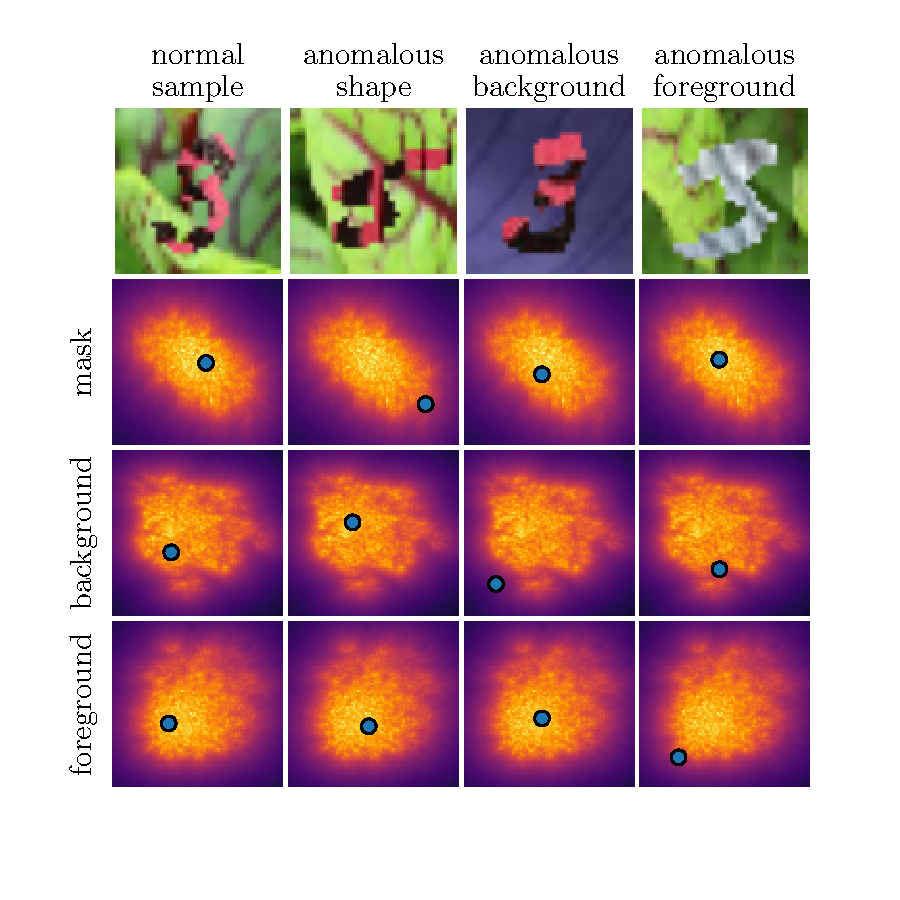
\includegraphics[width=0.95\textwidth]{data/chapter_sgvaegan/fig3_latent_decomposition_example.pdf}
    \caption{Position of different images encoded to individual latent spaces using SGVAEGAN model with two-dimensional latent spaces. The training set consisted of images with factors fixed to those of the digit in the first column. The densities of encodings of normal (training) data, estimated by a kNN detector~\eqref{eq:knnscore} are depicted as well.}
    \label{fig:latent_decomposition_example}
\end{figure}

If the SGVAEGAN is trained well, particularly if the decomposition into latent spaces is (at least approximately) right, different types of anomalies should be in low-density regions of different latent spaces. This is illustrated in Fig.~\ref{fig:latent_decomposition_example} on the Wildlife MNIST dataset, where we can see that anomalous shape, background texture, and foreground texture is anomalous in the corresponding latent space. We can use the score~\eqref{eq:alphadeco} and assign $p_{n_i}(\vc{z}_i) = p_{z_i}(\vc{z}_i), i \in \lbrace m,f,b \rbrace$, since the model is trained on normal data. Then we have
\begin{equation}
s(\vc{x}) = - \log p(\vc{e})  - \log\left\vert \frac{\partial g^{-1}(\vc{x})}{\partial \vc{x}}\right\vert -  \sum_{i\in\{m,f,b\}}\alpha_{i}\log p_{z_{i}}(\vc{z}_{i}),  
\label{eq:scorewithx}
\end{equation}
where $g(\vc{z})$ is a function that computes an image from the latent encodings via~\eqref{eq:composition}
\begin{equation}
g(\vc{z}) = g(\vc{z}_m, \vc{z}_f, \vc{z}_b) = g_{m, \vc{\theta}}(\vc{z}_m) \odot g_{f, \vc{\theta}}(\vc{z}_f) + (1 - g_{m, \vc{\theta}}(\vc{z}_m)) \odot g_{b, \vc{\theta}}(\vc{z}_b).
\end{equation}
Following the derivations in~\cite{vsmidl2019anomaly}, we use the fact that $\frac{\partial g^{-1}(\vc{x})}{\partial \vc{x}} = \left( \frac{\partial g(\vc{z})}{\partial z} \right) ^{-1}$, and assume the independency of the latent spaces of $\vc{z}_m, \vc{z}_f, \vc{z}_b$. Then Eq.~\eqref{eq:scorewithx} can be rewritten to 
\begin{align} \label{eq:scorejacodeco}  
s(\vc{x}) & = - \log p(e)  + s_j(\vc{x}) -  \sum_{i\in\{m,f,b\}} \alpha_{i}\log p_{z_{i}}(\vc{z}_{i}),
\end{align}
where $s_j(\vc{x}) = \log \left\vert  \frac{\partial g(\vc{z})}{\partial \vc{z}}  \right\vert $ denotes the Jacobian term, which is functionally dependent on the input image $\vc{x}$ through the latent encodings $\vc{z} = (\vc{z}_m, \vc{z}_f, \vc{z}_b)$, see~\eqref{eq:encoder}. A reader recognizes that $\frac{\partial g(\vc{z})}{\partial \vc{z}}$ is not square, hence its determinant is zero. Ref.~\cite{vsmidl2019anomaly} suggests estimating the determinant from a diagonal matrix after SVD decomposition, which is valid if one assumes the orthogonality of the data and noise.

The proposed score, based on~\eqref{eq:scorejacodeco}, reads as a weighted sum of the individual components
\begin{equation} \label{eq:totalscorejacobian}
    s(\vc{x}) = \alpha_{r}  s_{r}(\vc{x}) + \alpha_j s_j(\vc{x}) + \alpha_m s_{m}(\vc{x}) + \alpha_f s_{f}(\vc{x}) + \alpha_b s_{b}(\vc{x}),
\end{equation}
where $s_i, i \in \{r, j, m, f, b\}$ are individual anomaly score components which will be described in the following text. The $\alpha_r, \alpha_j$ weights were added in order to tune the total score to the modalities of anomalous data, which were not seen during the training, and therefore the base model is not fitted to them. The values of $\alpha$ can be either set manually or estimated from a small number of labeled anomalies as described in the following text.

\paragraph{Reconstruction error}
Reconstructed samples are needed for the computation of the reconstruction term $-\log p(\vc{e})$. However, since the reconstruction steps~\eqref{eq:encoder}-\eqref{eq:composition} contain sampling through the reparametrization trick, the reconstructions $\vc{x}'$ are stochastic. As we have shown already in~\eqref{eq:score_sample}, the estimate of the reconstruction error is stabilized by taking an average from multiple reconstructions $\lbrace \vc{x}'_l \rbrace_{l=1}^L$ computed as
\begin{equation} \label{eq:rsscore}
    s_{\text{r}}(\vc{x}) = - \frac{1}{\vc{\sigma}^2 L}\sum_{l=1}^L \vert \vert \vc{x}-\vc{x}'_l\vert \vert_2^2,
\end{equation}
where the scalar variance $\vc{\sigma}^2 \in \mathbb{R}$ is estimated from the data during the training of the model. The number of samples was set to $L=10$ during our experiments. 

\paragraph{Latent scores} A correct estimate of the likelihood of latent representations $p_{z_{i}}(\vc{z}_i),$ $i \in \{m, f, b\}$ is important for the score~\eqref{eq:totalscorejacobian}. Even though latent representations are regularized during the fitting of the model to have normal distribution $\mathcal{N}(0,\textbf{I})$, it was shown~\cite{dai2019diagnosing} that the fit is usually not very good. This can be also seen in Fig.~\ref{fig:latent_decomposition_example}, where the distribution of the latent representations is not perfectly normal. Therefore, we approximate $p_{z_{i}}(\vc{z}_i)$ by the k-nearest-neighbor (kNN) density estimator, see Sec.~\ref{sec:distance_methods}, which is trained on latent representations of normal data. This method was chosen for its simplicity yet powerful performance, which was demonstrated both by the results in Sec.~\ref{sec:alfven} and also in Chapter~\ref{sec:chapter_comparison}, where it scored amongst the top models on low dimensional data. This requirement will be satisfied here, as the encoders comprise the high-dimensional image data into latent space with dimensionality on the order of 10$^2$. The score of a sample in the $i$-th latent space, $i \in \lbrace m, f, b \rbrace$, has the form
\begin{equation} \label{eq:knnscore}
    s_{i}(\vc{x}) = \frac{1}{k} \sum_{\vc{z}_j \in \mathcal{Z}_{k,i}} \vert \vert \vc{z}_i - \vc{z}_j \vert \vert_2, \vc{z}_i = \vc{\mu}_{i,\vc{\phi}}(\vc{x}), 
\end{equation}
which is the average Euclidean distance between the projection $\vc{z}_i$ of the tested sample $\vc{x}$ into the latent space, and the set $\mathcal{Z}_{k,i}$ of the $k$-nearest projections of the normal data to the same latent space. The value of $k$ is a hyperparameter tuned on the validation set.

\paragraph{Optimization of $\alpha$ } The proposed score is effectively a weighted sum of individual parts. In theory, one can set the weights $\alpha$ by themselves if one knows in which latent to expect the anomaly. Since this knowledge is rarely available, we estimate them from data (that contains examples of labeled anomalies) by regularized logistic regression as
\begin{equation} \label{eq:alpha_regression}
    \alpha^* = \arg \min_{\alpha} - \sum_n y_n \log \vc{\sigma} (s(\vc{x}_n\vert\alpha)) + (1-y_n) \log(1-\vc{\sigma} (s(\vc{x}_n\vert\alpha)))) + \beta \vert \vert \alpha - \alpha_0 \vert \vert^2_2 ,
\end{equation}
\begin{equation}
    s(\vc{x}_n\vert\alpha) = \sum_i \alpha_i \hat{s}_i(\vc{x}_n), i \in \lbrace r, j, m, f, b \rbrace,
\end{equation}
where $\vc{\sigma}(.)$ is the sigmoid function, $y_n \in \lbrace 0,1 \rbrace$ are labels, $\alpha_0$ is a prior value and the index $n$ goes over the samples in the labeled dataset. Since the scores $s_i(\vc{x})$ can have very different scales (e.g. $s_r(\vc{x}) \sim 10^4$ while $s_f(\vc{x}) \sim 10^0$), we rescale them to have zero mean and unit variance. The rescaled scores are denoted as $\hat{s}_i(\vc{x})$. The regularization is set using $\beta = \frac{\beta_0}{n_1}, \beta_0 \in \mathbb{R}$, where $n_1$ is the number of positive (anomalous) samples in the dataset, and $\beta_0$ is a hyperparameter. This ensures that the prior $\alpha_0$ has a large influence over the final value of $\alpha$ when there is a small number of known anomalies, thus ensuring the robustness of the final $\alpha$ estimate. The prior is set such that $\alpha_{0,i}=1$ for such $i$ where the AUC computed from $\lbrace s_{i}(\vc{x}_n), y_n \rbrace_n$ is maximal and zero everywhere else, making $\alpha_0$ a failsafe value. The criterion~\eqref{eq:alpha_regression} is optimized by an LBFGS optimizer~\cite{liu1989limited}.

\paragraph{Removing the Jacobian from the score} 
While the score~\eqref{eq:scorejacodeco} is theoretically correct under the assumption that anomalies are located in areas of low density, the publication~\cite{vsmidl2019anomaly} shows that it does not work well when the model is trained on data without anomalies. Our experiments shown below arrived at the same conclusion. We suspect the cause to be that the decoders $g$ can be arbitrary (with arbitrary jacobian) in parts of the space not supported by the data, where anomalous samples are located. Moreover, the computation of the determinant is so expensive that the score is effectively useless for state-of-the-art image models. Therefore, we propose dropping the Jacobian term $s_j(\vc{x})$ from~\eqref{eq:totalscorejacobian} and adding the discriminator score
\begin{equation} \label{eq:discscore}
    s_d(\vc{x}) = 1 - d_{\vc{\varphi}}(\vc{x}),
\end{equation}
which works well for anomaly detection according to~\cite{larsen2016autoencoding} and also for semantic anomaly detection in images, which was shown by an exceptional performance of the fmGAN model with the score~\eqref{eq:discscore} in Chapter~\ref{sec:chapter_comparison}. The alternative score then reads
\begin{equation} \label{eq:totalscoredisc}
    s(\vc{x}) = \alpha_{r}  s_{r}(\vc{x}) + \alpha_d s_d(\vc{x}) + \alpha_m s_{m}(\vc{x}) + \alpha_f s_{f}(\vc{x}) + \alpha_b s_{b}(\vc{x}).
\end{equation}
Again, the values of $\alpha$ are optimized similarly to~\eqref{eq:alpha_regression}.

\subsection{Anomaly factor identification}
\label{sec:anomaly_factor_identification}
The model presented above can identify the source of the anomality through the information from the individual latent spaces. Under the formalism~\eqref{eq:pzy}, estimation of the probability of being generated from the normal model is simply $p(y \vert \vc{z})\propto p(\vc{z} \vert y)$, which is only possible for proper distributions. Since we used an improper distribution ($p_a(\vc{x})\propto 1$) to minimize the number of unknown parameters, we cannot use direct estimation and have to rely on approximation. This approximation relies on the fact that the source of anomaly should have a low probability in the respective latent space. We have designed two approximate methods for identifying it. The main benefit of these methods is that they are completely unsupervised and computationally cheap. Note that when using them, it is assumed that anomalies are generated from a single source, i.e. being anomalous only either in shape, foreground, or background. 

\paragraph{Ranked anomaly factor identification}
The first approximation relies on the replacement of the likelihood $p(y_i\vert \vc{z}_i(\vc{x}))$ by an empirical quantile.  Specifically, we store the values of anomaly scores $s_{i,train}=s_i(\vc{x}_{train})$ for the training set and for a new sample $\vc{x}$ compute the quantile $q_i(\vc{x})$ (relative rank) within the training scores of the corresponding latent space. The anomaly source estimate is then computed as the maximum of the relative rank $y^* = \arg\max_{i\in\{m,f,b\}}q_i(\vc{x})$.

\begin{figure}
    \centering
    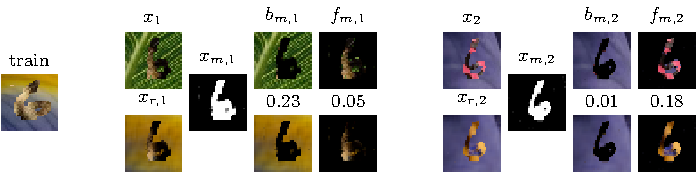
\includegraphics[width=0.95\textwidth]{data/chapter_sgvaegan/fig4_masked_examples.pdf}
    \caption{Masked detection technique for identifying the source of anomality. The model was originally trained on samples similar to the one on the very left, brown-striped sixes on a purple-yellow background. To distinguish between anomalies in the background and foreground texture, a reconstruction $\vc{x}_r$ and a mask $\vc{x}_m$ are computed for a test sample $\vc{x}_1$, which is anomalous in the background, and $\vc{x}_2$, which is anomalous in the foreground texture. The scores $S_b$ \eqref{eq:sb}, $S_f$ \eqref{eq:sf} are computed as scaled differences between the original and reconstructed masked--out backgrounds, $b_m = \vc{x} \odot (1-\vc{x}_m)$ and foregrounds $f_m = \vc{x} \odot \vc{x}_m$ and their values are displayed between the image of the original and reconstructed foregrounds and backgrounds.}
    \label{fig:masked_detection}
\end{figure}

\paragraph{Masked anomaly factor identification}
Using even a properly trained model, the ranked method is not always able to correctly identify all three types of anomaly sources. Therefore, we have simplified the problem to distinguish the source of an anomaly only in the background or foreground texture by computing the reconstruction errors for those components separately. For an input $\vc{x}$, the reconstructed image $\vc{x}'$ and a mask $\vc{x}_m$ are computed. Using these, we compute the normalized reconstruction errors as
\begin{align}
    S_b & = \frac{\sum_j \left( (\vc{x}_j-\vc{x}_{j}') (1-\vc{x}_{m,j}) \right) ^ 2}{\sum_j 1-\vc{x}_{m,j}} \label{eq:sb} \\
    S_f & = \frac{\sum_j \left( (\vc{x}_j-\vc{x}_{j}') \vc{x}_{m,j} \right) ^ 2}{\sum_j \vc{x}_{m,j}}  \label{eq:sf}
\end{align}
where index $j$ goes over elements in all dimensions of an array $\vc{x} \in \mathbb{R}^{H \times W \times 3}$ representing an RGB image. See Fig.~\ref{fig:masked_detection} for an illustration of the principle of this method. The normalization factor in (\ref{eq:sb},\ref{eq:sf}) is important since the object in the foreground usually covers fewer pixels than the background. If $S_b$ is higher, the prediction for the anomaly factor is "background" and vice versa. The comparison of the ranked and masked method is presented in Sec.~\ref{sec:anomaly_factor_identification_experiments}

%%%%%%%%%%%%%%%%%%%%%%%%%%%%%
% Experiments

\section{Experiments} \label{sec:experiments}

In the experimental evaluation of the proposed model, we follow the strict protocol that was established in Chapter~\ref{sec:chapter_comparison}. The datasets were split into training, validation, and test subsets for each of their classes (or subproblems in the case of the MVTec-AD dataset). Details on the splits for individual experiments can be found in the respective sections below. Then, for each such split and each model, 50 hyperparameter settings were randomly sampled from a set of possible values. The use of Bayesian optimization to select hyperparameters was considered but eventually dropped as it did not have an impact on the relative rank of the methods in Chapter~\ref{sec:chapter_comparison}. The validation set was used to select the best hyperparameter values for a given model on a specific subproblem. Unless mentioned otherwise, the experiments below report (ROC)AUC values of the selected models computed on the test set. The models were trained for 50 epochs each.

The datasets used in the experimental evaluation were selected in order to contain semantic anomalies (with the exception of the MVTec-AD dataset). Two artificial datasets (Wildlife MNIST and COCOPlaces) were created as baselines on which the model is supposed to perform well. Especially Wildlife MNIST contains easily segmentable objects. For details on datasets, see Appendix~\ref{sec:appendix_datasets}.

\subsection{Baseline methods}
We have selected unsupervised anomaly detectors mainly based on the review in Chapter~\ref{sec:chapter_comparison}, specifically those that were amongst the top performers on colored images. For additional These models include:

\begin{description}
    \item[\textbf{Variational Autoencoder (VAE)}] - a convolutional VAE from Sec.~\ref{sec:vae_models} that uses the sampled reconstruction error~\eqref{eq:rsscore}. The decoder variance $\vc{\sigma}^2$ is estimated from the data.
    \item[\textbf{Feature-matching GAN (fmGAN)}] - a convolutional GAN model trained using the feature-matching loss~\eqref{eq:fmgan}. The anomaly score is based on the discriminator~\eqref{eq:discscore}.
    \item[\textbf{VAEGAN}] - a  convolutional VAE where reconstruction is enforced through a discriminator~\cite{larsen2016autoencoding}. The anomaly score is~\eqref{eq:discscore}.
    \item[\textbf{Deep Support Vector Data Description (DSVDD)}] - is a model that learns a transformation of data via a neural network to a subspace where the anomalies lie outside of a hypersphere composed of transformed normal data. The anomaly score is then the distance of a point from the center of the hypersphere, see Sec.~\ref{ref:sec_deep_domain}.
    \item[\textbf{fast Anomaly GAN (fAnoGAN)}] - a GAN model trained via Wasserstein loss and gradient penalization that identifies anomalies by backward-searching the latent code $z$ that is the most likely to generate the given test samples, see Sec.~\ref{sec:gan_survey}.
    \item[\textbf{Counterfactual Generative Network (CGN)}] - this is a baseline model~\cite{sauer2021counterfactual} for the decomposition of data into three components. Although not originally intended as an anomaly detector, it can be used as one as it provides the discriminator score~\eqref{eq:discscore} and proved itself to be competitive in our experiments.
    \item[\textbf{Shape Guided VAE (SGVAE)}] - this is a modification of the proposed model introduced to study the impact of the discriminator. It is trained without a discriminator and the reconstruction loss is $ -\mathbb{E}_{q_{\vc{\phi}}(\vc{z} \vert \vc{x})}[\log p_{\vc{\theta}}(\vc{x} \vert \vc{z})]$, similar to a classical VAE. The anomaly score for this model is the sampled reconstruction error~\eqref{eq:rsscore}.
    \item[\textbf{Shape Guided VAEGAN (SGVAEGAN)}] - this is the basic proposed model that is trained in a completely unsupervised fashion and evaluated without considering the full anomaly scores~\eqref{eq:totalscorejacobian} and~\eqref{eq:totalscoredisc}. Instead, the default anomaly score is~\eqref{eq:discscore}.
    \item[\textbf{SGVAE$_{\alpha}$}] - this is the SGVAE model where the score~\eqref{eq:totalscorejacobian} is considered. To compute the anomaly scores,  SGVAE models pre-trained in an unsupervised fashion were used and only the weights $\alpha$ were computed on a validation dataset.
    \item[\textbf{SGVAEGAN$_{\alpha}$}] - this is the full proposed model. As discussed in the Sec.~\ref{sec:jacobian_contribution}, it is used with the score~\eqref{eq:totalscorejacobian} with the Jacobian, but later the Jacobian is dropped and the model is used with score~\eqref{eq:totalscoredisc}.
\end{description}
    
\subsection{The contribution of the Jacobian} \label{sec:jacobian_contribution}
\begin{table}[t] 
 \center 
 \begin{tabular}{c c c c c } 
 \toprule 
  class & AUC - no $s_j(x)$ & AUC - with $s_j(x)$ & $\alpha_r$ & $\alpha_j$  \\ 
  \midrule
  0 & 0.70 $\pm $0.04 & 0.70 $\pm $0.05 & 1.00 & 0.00  \\ 
  1 & 0.82 $\pm $0.01 & 0.82 $\pm $0.02 & 1.09 & -0.03  \\ 
  2 & 0.71 $\pm $0.02 & 0.72 $\pm $0.02 & 0.93 & -0.01  \\ 
  3 & 0.64 $\pm $0.02 & 0.64 $\pm $0.02 & 0.94 & 0.01  \\ 
  4 & 0.72 $\pm $0.03 & 0.72 $\pm $0.03 & 1.00 & 0.00  \\ 
  5 & 0.67 $\pm $0.01 & 0.66 $\pm $0.01 & 0.98 & 0.00  \\ 
  6 & 0.68 $\pm $0.02 & 0.68 $\pm $0.02 & 0.60 & 0.00  \\ 
  7 & 0.73 $\pm $0.05 & 0.73 $\pm $0.05 & 1.00 & 0.00  \\ 
  8 & 0.69 $\pm $0.04 & 0.71 $\pm $0.02 & 0.98 & -0.04  \\ 
  9 & 0.63 $\pm $0.05 & 0.63 $\pm $0.04 & 0.80 & 0.00  \\ 
  \bottomrule
 \end{tabular}
 \caption{Experiment with $s_j(x)$ on a subset of the SVHN2 dataset. The mean values of  $\alpha$ weights estimated with~\eqref{eq:alpha_regression} are also presented and show that the weight of the Jacobian term is suppressed during their computation.} 
 \label{tab:jacoceco_partial_experiment} 
\end{table}
We start by demonstrating that dropping the Jacobian term from the score~\eqref{eq:totalscorejacobian} does not have a negative effect on the detection performance of the proposed model. Tab.~\ref{tab:jacoceco_partial_experiment} shows AUCs of the model that uses the score~\eqref{eq:totalscorejacobian} with and without the Jacobian term $s_j(\vc{x})$ on a subset of the SVHN2 dataset. For each normal class, training, and testing sets containing 750 normal and 150 anomalous samples were used. To obtain the presented statistic, the subsets were sampled 5 times.  The difference in performance is almost negligible but the difference in computational costs is high. Therefore, we omit the term from all further experiments, and the score~\eqref{eq:totalscoredisc} is used for the SGVAEGAN$_{\alpha}$ instead, while for SGVAE$_\alpha$, the term is dropped from~\eqref{eq:totalscorejacobian}.

\subsection{Detection of semantic anomalies} 
\begin{figure}[ht!]
    \centering
    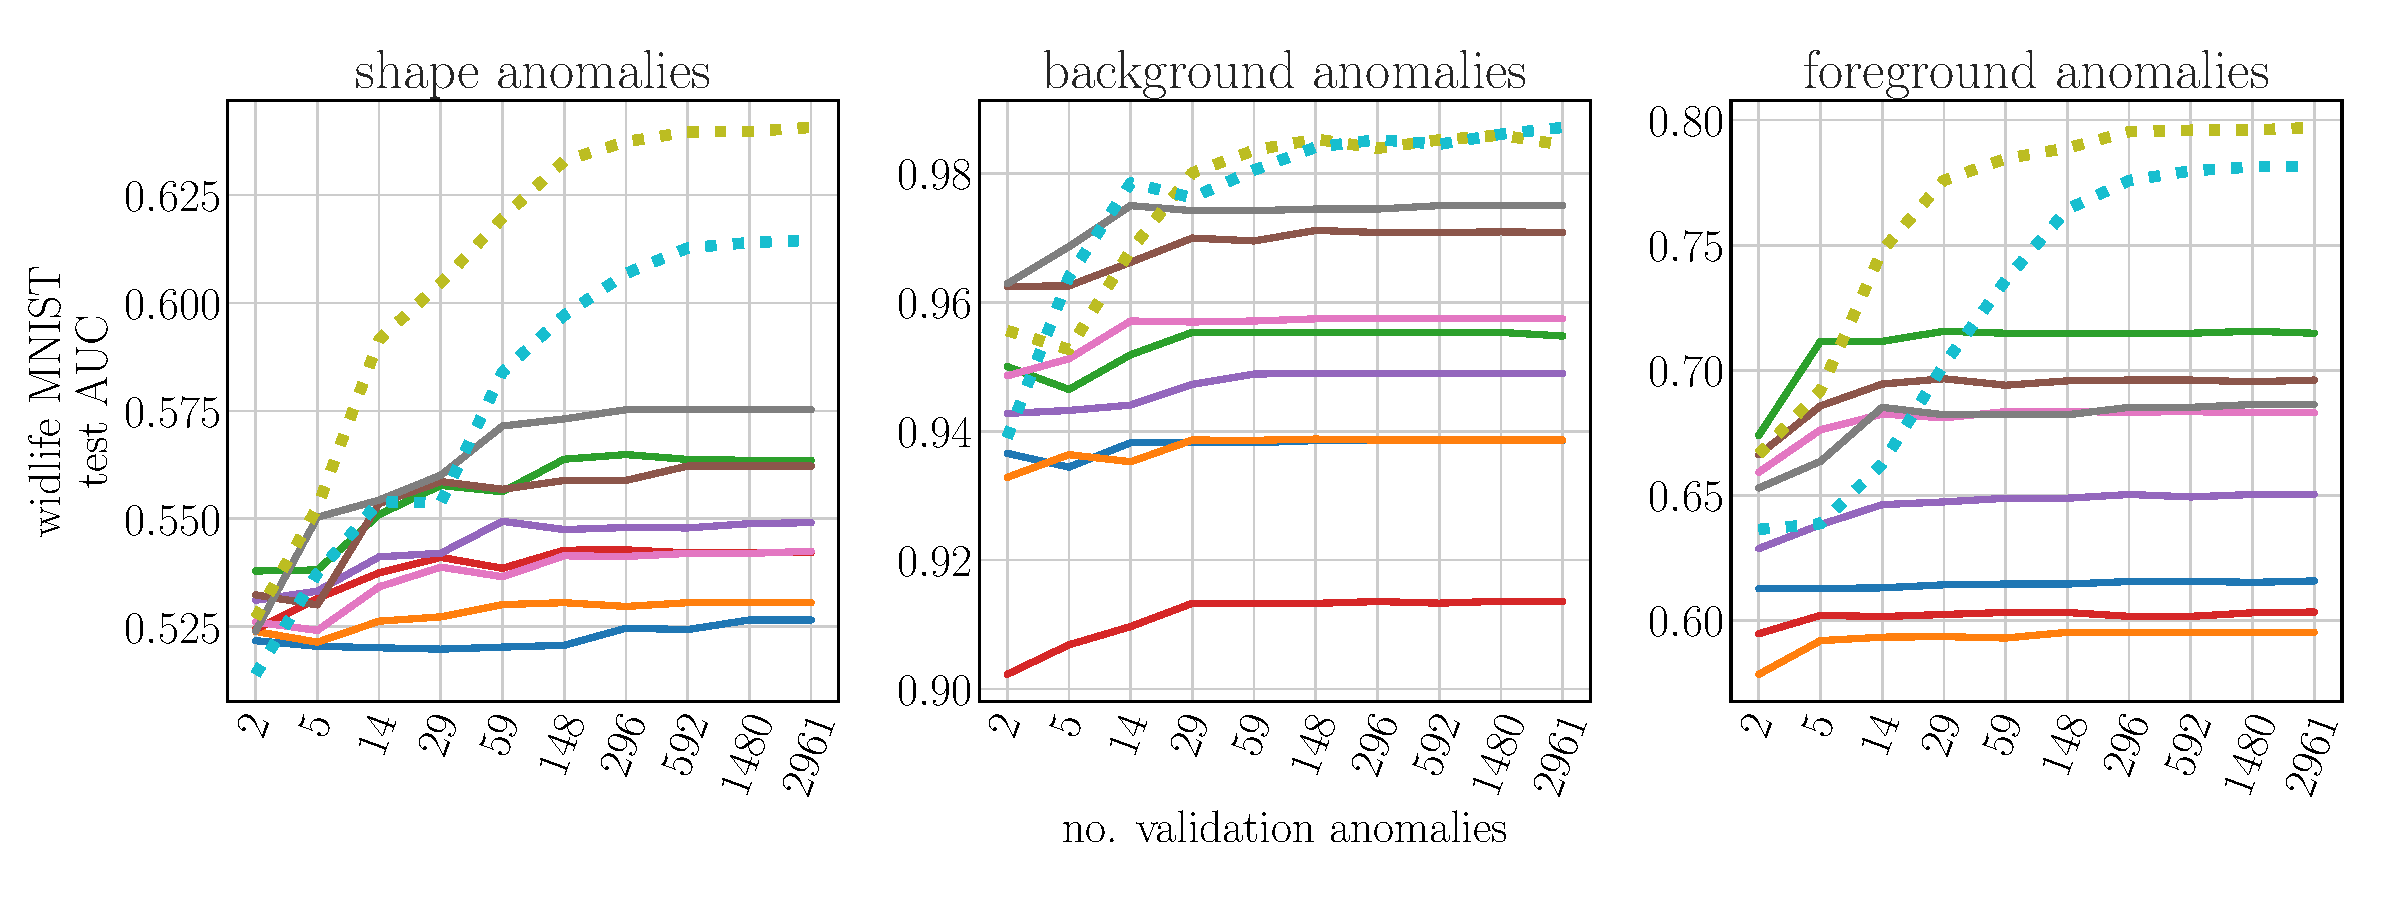
\includegraphics[width=\textwidth]{data/chapter_sgvaegan/fig6_multifactor_experiments_wmnist.pdf}
    
    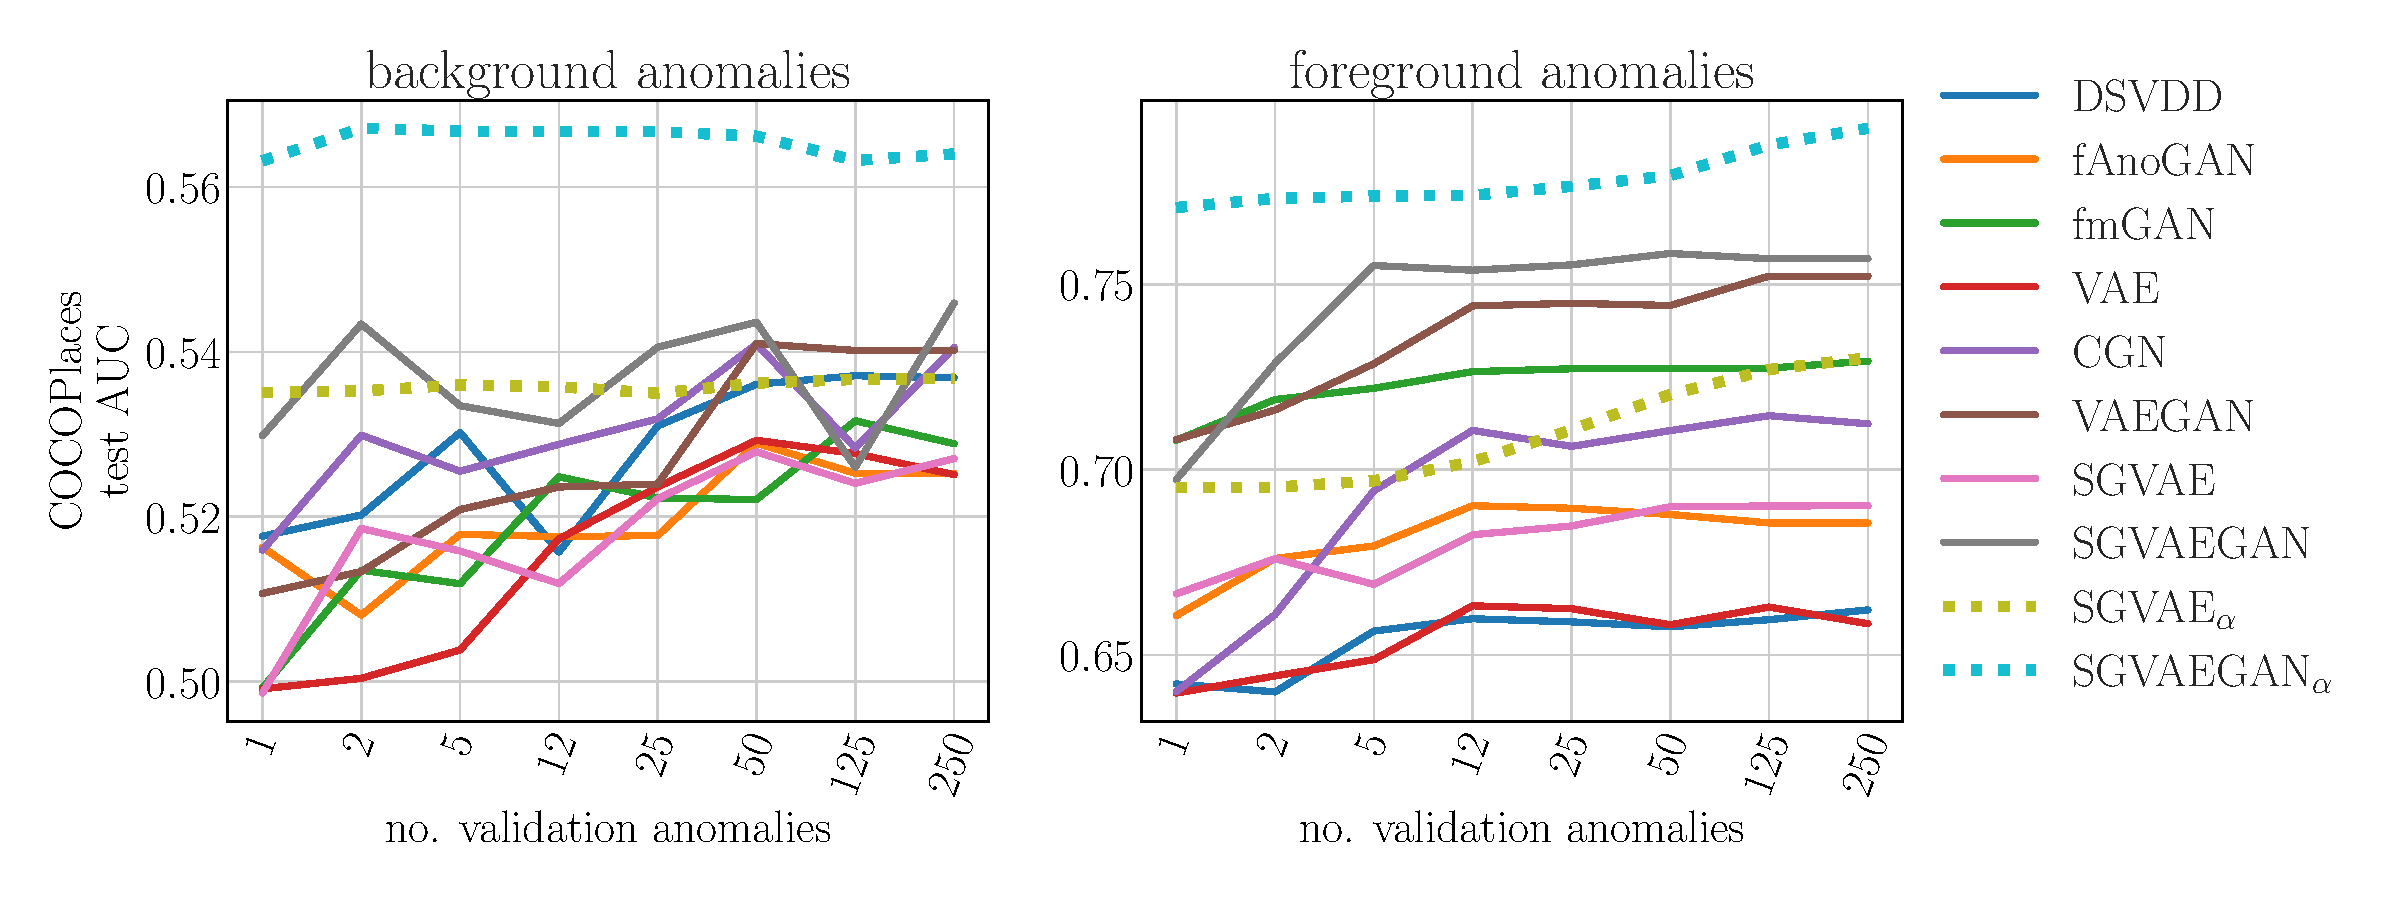
\includegraphics[width=\textwidth]{data/chapter_sgvaegan/fig7_multifactor_experiments_coco.pdf}
    \caption{Semantic anomaly detection experiment on the Wildlife MNIST (top) and COCOPlaces (bottom) datasets. The x-axis covers a changing number of anomalies present in the validation dataset. The y-axis reports the average AUC over dataset subclasses and 5-fold cross-validation.}
    \label{fig:multifactor}
\end{figure}
We now study how the proposed detector behaves as it gradually incorporates more knowledge in the form of labeled anomalies used to optimize weights $\alpha$ via~\eqref{eq:alpha_regression}. To simulate a semantic anomaly scenario, the following training and testing protocol is used with the Wildlife MNIST and COCOPlaces datasets. The training set consists of samples of one class (the whole experiment is repeated for all 10 classes) from the non-mixed version of the datasets (see Appendix.~\ref{sec:appendix_datasets} for details of how this is generated). Then, for a given factor of variation, validation, and test sets are drawn from the mixed version of the dataset, where the anomality of a sample is based on whether the target factor is the same or different as in the training dataset. This introduces a non-semantic shift, as the validation and test sets contain a variation of a factor that was not seen in the training data but is not considered anomalous. 

An example of how the individual data sets are constructed is the following: consider that the training set contains only images of MNIST class "0" with "leaf" background and brown foreground texture, like in Fig.~\ref{fig:wmnist_grid}. When the target factor of variation is \textit{background}, then in the validation and test set, all images with "leaf" background are considered normal and any other background is considered anomalous, no matter what the remaining factors of variation (digit and foreground texture) are, therefore a brown digit "0" with a blue background texture is considered anomalous, while a yellow "9" with "leaf" background is considered normal.

Fig.~\ref{fig:multifactor} shows AUCs of compared methods with respect to the number of known anomalies in the validation set, in which the ratio of anomalous to normal data ranges from 0.1\% to 100\% with the number of normal samples staying the same. The models are trained on the same training non-mixed data, their hyperparameters are selected on the validation dataset and the resulting test set AUC is averaged over 10 classes and a 5-fold random selection of the validation anomalies. While on Wildlife MNIST, both SGVAE$_\alpha$ and SGVAEGAN$_\alpha$ quickly dominate other methods once a few (five) examples of anomalies are available, the SGVAE$_\alpha$ performs worse on COCOPlaces. This is the effect of the discriminator of SGVAEGAN, which is used in the score and which contributes to the improved fit of the model. The results also show how methods benefit from a better selection of hyperparameters when more known anomalies are in the validation set.

\subsection{Anomaly factor identification} \label{sec:anomaly_factor_identification_experiments}
In this section, we compare the two approximate methods for identification of the source of an anomaly as described in Sec.~\ref{sec:anomaly_factor_identification}, i.e. the ranked and the masked method. For the comparison, we use the mixed version of the Wildlife MNIST dataset. The results in the form of prediction accuracies over different normal classes are shown in~Tab.~\ref{tab:factor_detection}. 

\begin{table}[h] 
 \center 
 \begin{tabular}{c | c c c | c c}
 \toprule
 & \multicolumn{3}{c|}{ranked} & \multicolumn{2}{c}{masked} \\
  normal class & shape & background & foreground & background & foreground  \\ 
  \midrule 
  0 & 0.82 & 0.19 & 0.62 & 0.88 & 0.95  \\ 
  1 & 0.84 & 0.92 & 0.19 & 0.85 & 1.0  \\ 
  2 & 0.92 & 0.37 & 0.7 & 0.95 & 0.6  \\  
  3 & 0.55 & 0.86 & 0.24 & 0.63 & 0.96  \\
  4 & 0.79 & 0.46 & 0.85 & 0.62 & 1.0  \\ 
  5 & 0.57 & 0.89 & 0.31 & 0.72 & 1.0  \\ 
  6 & 0.74 & 0.95 & 0.52 & 0.96 & 0.96  \\
  7 & 0.47 & 0.84 & 0.75 & 0.87 & 0.98  \\
  8 & 0.64 & 0.64 & 0.62 & 0.98 & 0.97  \\
  9 & 0.88 & 0.27 & 0.1 & 0.77 & 0.94  \\
   \bottomrule
 \end{tabular}
 \caption{Accuracy of factor detection on the wildlife MNIST dataset for \textit{ranked} and \textit{masked} methods. The columns correspond to test samples anomalous in the respective factor.} 
 \label{tab:factor_detection} 
\end{table}

The ranked method sometimes fails to identify all three factors better than random chance, which has an accuracy of 0.33. The masked method performs better than the ranked one in the identification of the background and foreground anomalies, although the background anomaly detection accuracies are not completely satisfactory on all digit classes. However, we explain this by some classes having very similar backgrounds, e.g. a very common misclassification for class "4" is that with anomalous background from classes "1" or "7", see~Fig.~\ref{fig:wmnist_grid}. In these misclassifications, the background is reconstructed rather well, while even a small imprecision in the mask leads to a high reconstruction error in the foreground. Still, this method of detection of the source of anomality might be useful in some real-world problems, given we can train the model to produce correct masks. 

\subsection{Large scale study} \label{sec:benchmarks}
\begin{figure}[ht!]
    \centering
        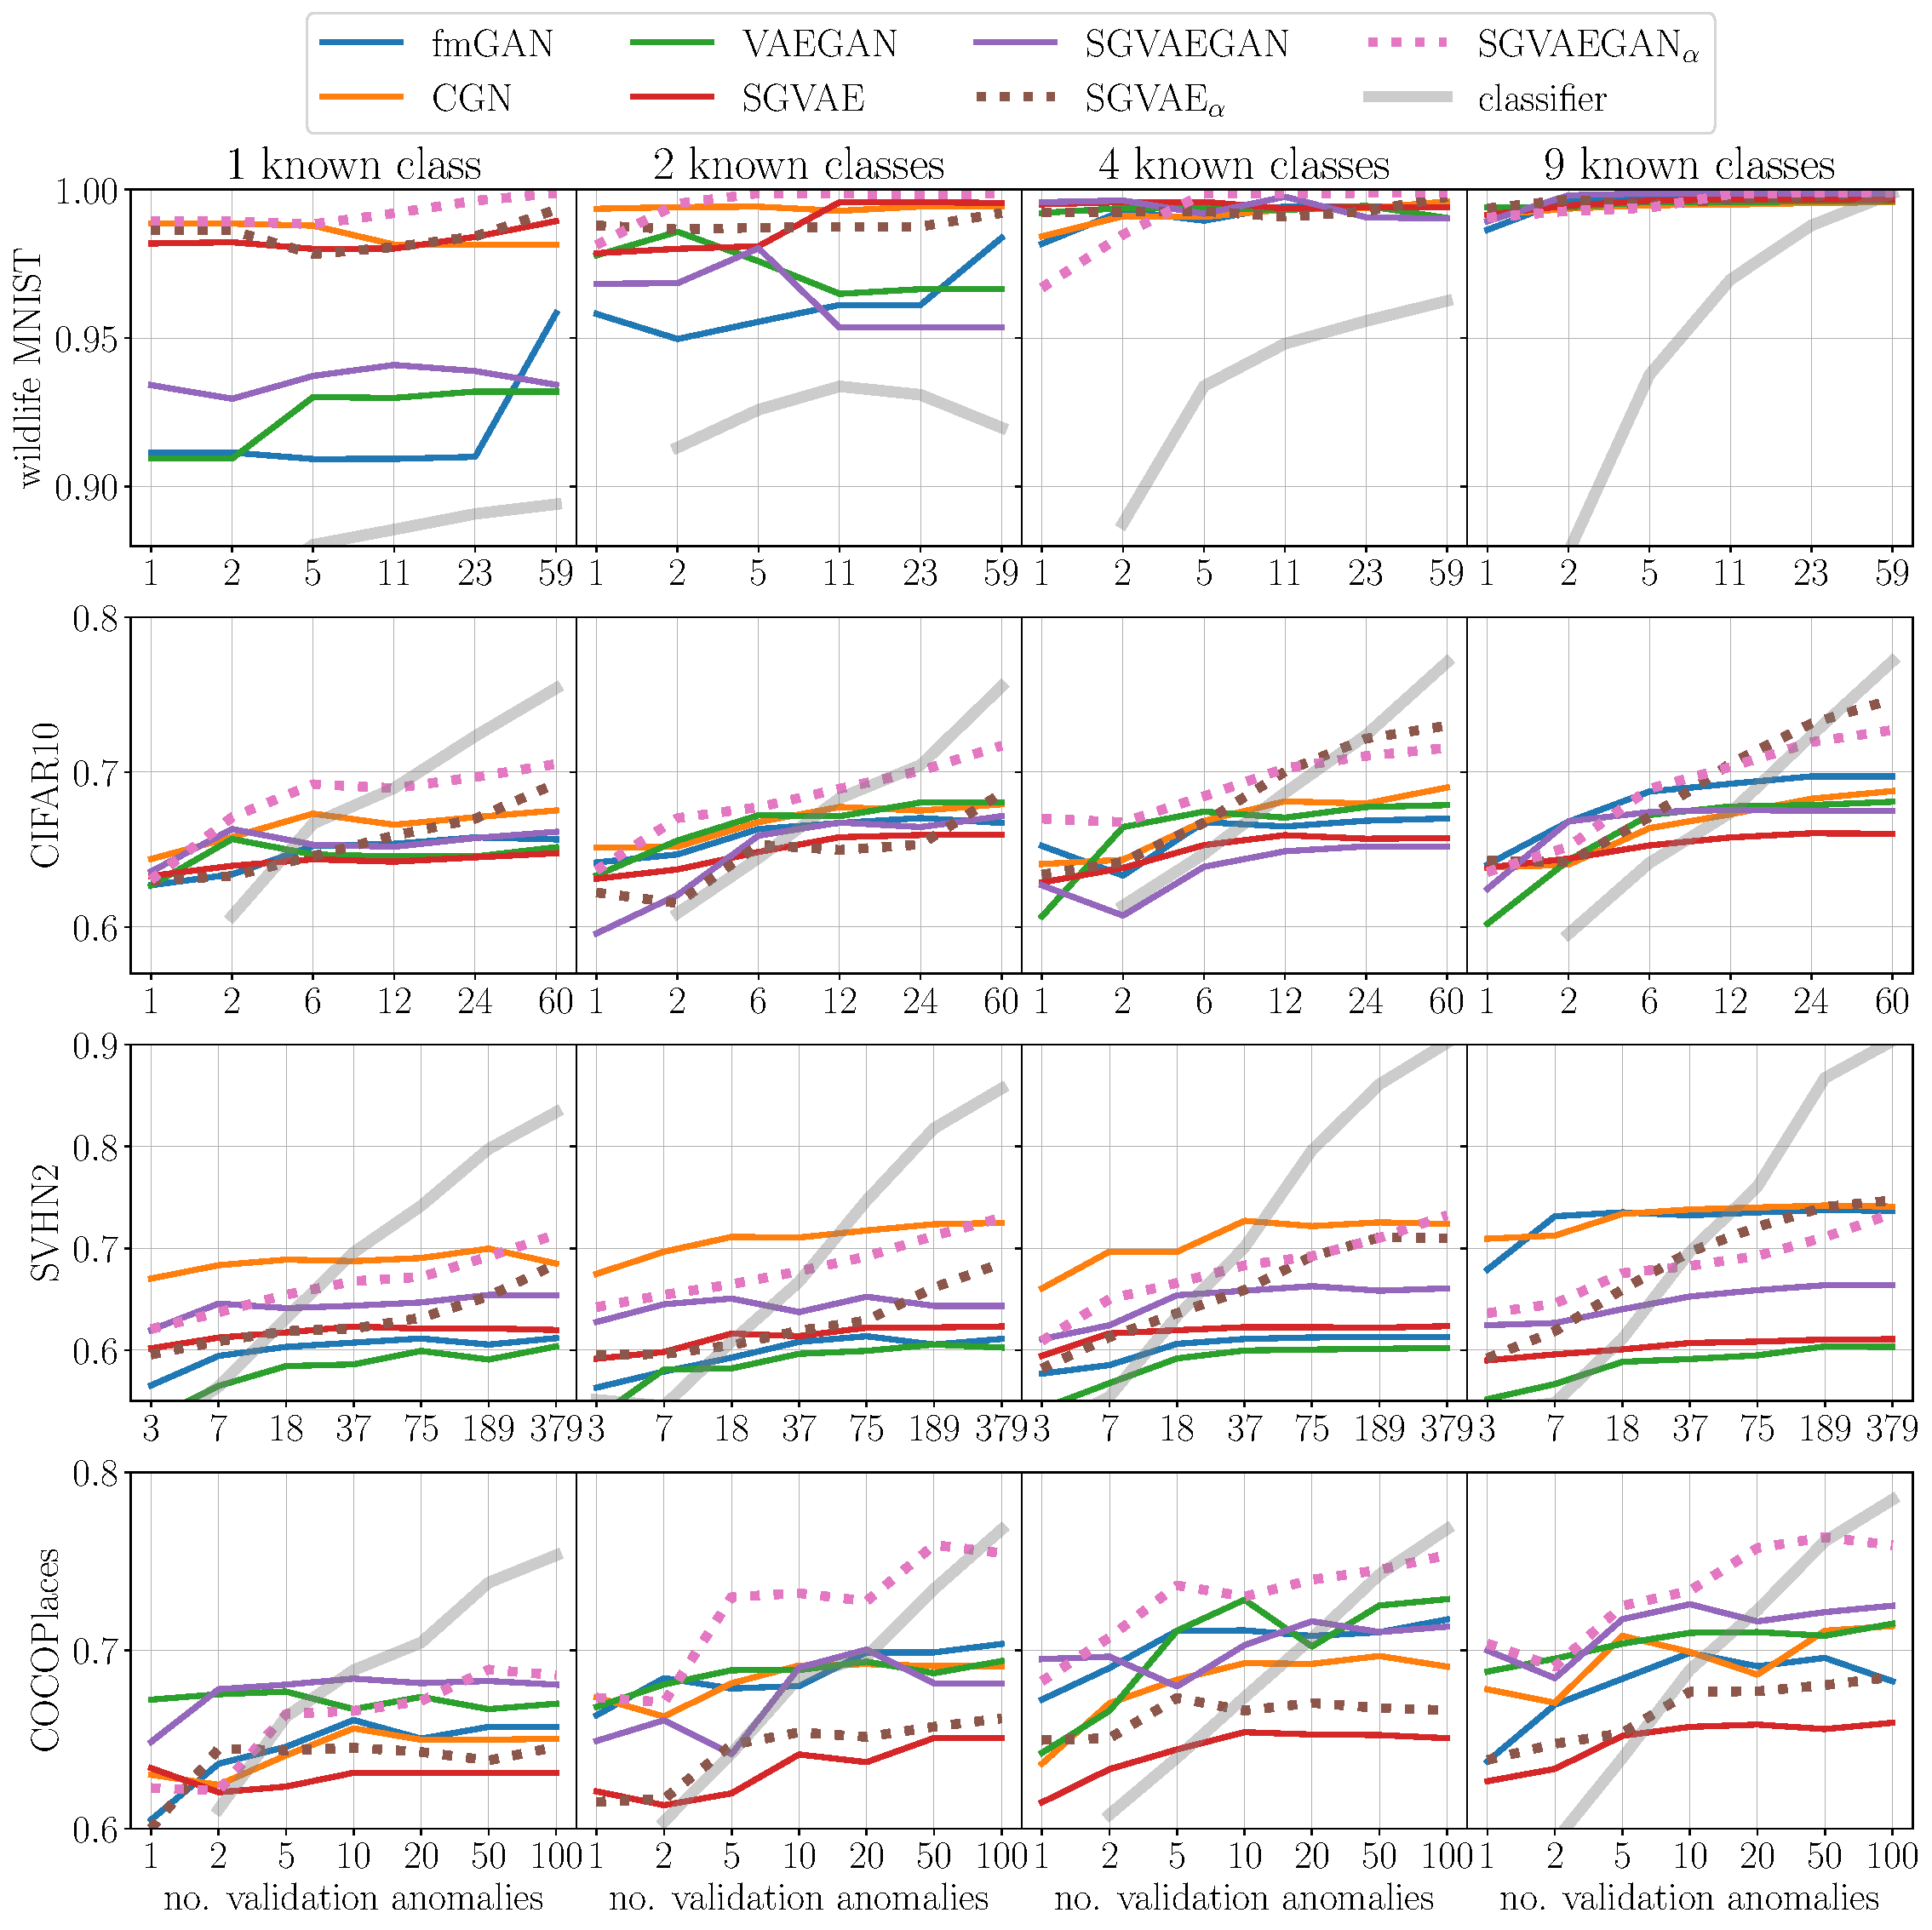
\includegraphics[width=\textwidth]{data/chapter_sgvaegan/fig8_all.pdf}
    \caption{Comparison of models on selected image datasets for the leave-one-in experiment. The x-axis covers a changing number of anomalies in the validation dataset, which is used for hyperparameter selection and $\alpha$ computation. The y-axis reports the average test AUC over 10 normal classes. The columns capture experiments with varying availability of validation samples from different anomalous classes, while anomalies of all classes are present in the test set. The number of normal samples in the validation set is the following: Wildlife MNIST: 1184, CIFAR10: 1200, SVHN2: 3792, COCOPlaces: 100.}
    \label{fig:kplots}
\end{figure}

\begin{table}[ht!] 
 \center 
 \begin{tabular}{c c c c c c c c c c c } 
  problem & \rotatebox{90}{DSVDD} & \rotatebox{90}{fAnoGAN} & \rotatebox{90}{fmGAN} & \rotatebox{90}{VAE} & \rotatebox{90}{CGN} & \rotatebox{90}{VAEGAN} & \rotatebox{90}{SGVAE} & \rotatebox{90}{SGVAEGAN} & \rotatebox{90}{SGVAE$_{\alpha}$} & \rotatebox{90}{SGVAEGAN$_{\alpha}$}  \\ 
  \midrule 
  bottle & 0.81 & \cellcolor{gray!30} 0.97 & \cellcolor{gray!15} 0.95 & \cellcolor{gray!45} 0.98 & 0.90 & 0.85 & \cellcolor{gray!45} 0.98 & 0.83 & \cellcolor{gray!30} 0.97 & 0.92  \\ 
  capsule & 0.65 & 0.69 & 0.67 & \cellcolor{gray!15} 0.74 & 0.69 & 0.58 & \cellcolor{gray!30} 0.76 & 0.66 & \cellcolor{gray!45} 0.80 & 0.67  \\ 
  nut & 0.78 & 0.72 & \cellcolor{gray!45} 0.88 & 0.71 & 0.82 & \cellcolor{gray!15} 0.84 & 0.69 & 0.78 & 0.81 & \cellcolor{gray!30} 0.86  \\ 
  pill & 0.64 & 0.71 & \cellcolor{gray!15} 0.73 & \cellcolor{gray!15} 0.73 & 0.59 & 0.70 & \cellcolor{gray!30} 0.77 & 0.72 & \cellcolor{gray!45} 0.78 & \cellcolor{gray!15} 0.73  \\ 
  transistor & 0.69 & 0.77 & \cellcolor{gray!45} 0.90 & \cellcolor{gray!15} 0.81 & \cellcolor{gray!30} 0.88 & 0.75 & 0.78 & 0.79 & \cellcolor{gray!15} 0.81 & 0.79  \\ 
  \midrule
  mean rank & 8.90 & 6.20 & \cellcolor{gray!30} 3.50 & \cellcolor{gray!15} 4.20 & 5.50 & 7.60 & 4.50 & 7.00 & \cellcolor{gray!45} 2.80 & 4.80  \\ 
  \bottomrule
 \end{tabular}
 \caption{Aggregated performance in test AUC of models on MVTec-AD problems.} 
 \label{tab:mvtec} 
\end{table}

\begin{figure}[ht!] 
    \centering
    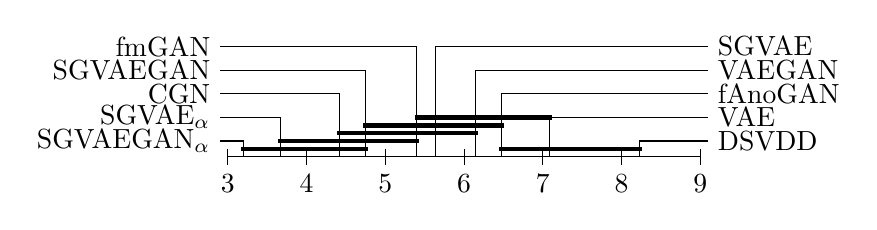
\begin{tikzpicture}[scale=1.0] 
  \draw (3.0,0) -- (9.0,0); 
  \foreach \x in {3,...,9} \draw (\x,0.10) -- (\x,-0.10) node[anchor=north]{$\x$}; 
  \draw (3.2,0) -- (3.2,0.19999999999999998) -- (2.9, 0.19999999999999998) node[anchor=east] {SGVAEGAN$_{\alpha}$}; 
  \draw (3.6625,0) -- (3.6625,0.5) -- (2.9, 0.5) node[anchor=east] {SGVAE$_{\alpha}$}; 
  \draw (4.4125,0) -- (4.4125,0.7999999999999999) -- (2.9, 0.7999999999999999) node[anchor=east] {CGN}; 
  \draw (4.75,0) -- (4.75,1.0999999999999999) -- (2.9, 1.0999999999999999) node[anchor=east] {SGVAEGAN}; 
  \draw (5.4,0) -- (5.4,1.4) -- (2.9, 1.4) node[anchor=east] {fmGAN}; 
  \draw (5.6375,0) -- (5.6375,1.4) -- (9.1, 1.4) node[anchor=west] {SGVAE}; 
  \draw (6.15,0) -- (6.15,1.0999999999999999) -- (9.1, 1.0999999999999999) node[anchor=west] {VAEGAN}; 
  \draw (6.475,0) -- (6.475,0.8) -- (9.1, 0.8) node[anchor=west] {fAnoGAN}; 
  \draw (7.0875,0) -- (7.0875,0.5) -- (9.1, 0.5) node[anchor=west] {VAE}; 
  \draw (8.225,0) -- (8.225,0.2) -- (9.1, 0.2) node[anchor=west] {DSVDD}; 
  \draw[line width=0.06cm,color=black,draw opacity=1.0] (3.170000047683716,0.1) -- (4.78,0.1); 
  \draw[line width=0.06cm,color=black,draw opacity=1.0] (3.6324999046325686,0.2) -- (5.430000095367432,0.2); 
  \draw[line width=0.06cm,color=black,draw opacity=1.0] (4.382499904632568,0.30000000000000004) -- (6.180000095367432,0.30000000000000004); 
  \draw[line width=0.06cm,color=black,draw opacity=1.0] (4.72,0.4) -- (6.504999904632569,0.4); 
  \draw[line width=0.06cm,color=black,draw opacity=1.0] (5.370000095367431,0.5) -- (7.117500095367432,0.5); 
  \draw[line width=0.06cm,color=black,draw opacity=1.0] (6.444999904632568,0.1) -- (8.255000381469726,0.1); 
 \end{tikzpicture} 

    \caption{A critical difference diagram that shows mean ranks of models from Tab.~\ref{tab:loi_ranks_per_ac}. The difference in the performance of 2 models compared on 40 datasets to be statistically significant on level 10\% must be greater than the value of the Nemenyi test $CD_{0.1}$=1.95. The thick horizontal lines connect the models with performance differences less than this.}
    \label{fig:cd}
\end{figure}

This experiment compares the proposed model in a traditional anomaly detection scenario on selected image datasets. We assume the leave-one-in scenario, when the training dataset contains samples from one class and the rest is considered to be anomalous in validation and test datasets. We believe this is a good representation of a semantic anomaly detection problem as well as being a more realistic option since in real-world problems, anomalies may come from many varying distributions.\footnote{In this regard, we disagree with the authors of~\cite{ahmed2020detecting} which propose the alternative of leave-one-out, stating that in most anomaly detection problems, we want to detect only small perturbations from the target class. However, traditional image benchmarks don't allow for this anyway as the classes are very distinct even in the latter case.} To test the models in a non-semantic anomaly detection setting, we have included the MVTec-AD dataset where the normal and anomalous data differ only in small details, and which is popular for benchmarking anomaly detection methods.

In practice, it might happen that anomalies are in a few clusters, but only samples from some of them are labeled and available for model selection. To simulate such a scenario and similar validation/test discrepancies, we performed model selection with significantly varied validation sets. First, the total number of anomalies in the validation set was varied, which constitutes the x-axis in Fig.~\ref{fig:kplots}. Second, for each normal class, samples from only a limited number of anomalous classes were sampled to the validation set, which creates the different columns in Fig.~\ref{fig:kplots}. The test set contained anomalies from all the classes left out of training. An example with 4 anomalous classes known in validation: training of models was done using class "1" of the SVHN2 dataset. The validation dataset contained normal data from class "1" and anomalies sampled from classes "2", "3", "4" and "5". The testing dataset contained normal samples from class "1" and anomalies sampled from all the other classes. The normal data split is 60/20/20\%, 50\% of available anomalies are in the test set. 

Fig.~\ref{fig:kplots} contains the overall comparison across the different variants of validation datasets used for model selection. It contains only a selection of the best-performing models to improve readability. Apart from the SVHN2 dataset, the proposed model outperforms the baselines after observing just 10 examples of anomalies, in some cases even less. A comparison of all baselines aggregated over all semantic datasets is presented in the critical difference diagram in Fig.~\ref{fig:cd}, where mean ranks of models are compared using the methodology presented in~\cite{demsar2006statistical}. Tab.~\ref{tab:loi_ranks_per_ac} contains a disaggregated comparison in the case of 2\% of labeled anomalies from 4 classes in the validation dataset. Finally, see Tab.~\ref{tab:mvtec} for the results on the MVTec-AD subproblems. Here the alternative SGVAE$_{\alpha}$ trained without a discriminator performs better. This is probably because the dataset only contains non-semantic anomalies, which cannot be well captured by the discriminator score which is used in SGVAEGAN$_{\alpha}$. Since the total number of anomalies in MVTec-AD is low, the use of the discriminator score may lead to overfitting of the $\alpha$ estimate on the validation dataset. By selecting the optimal model on the validation set and reporting on the test set, which is not standard in every publication~\cite{vskvara2021comparison}, we believe that our experiments provide a realistic comparison of baselines.

\begin{table}[ht!] 
 \center 
 \resizebox{\textwidth}{!}{ 
 \begin{tabular}{c c c c c c c c c c c c } 
  & class & \rotatebox{90}{DSVDD} & \rotatebox{90}{fAnoGAN} & \rotatebox{90}{fmGAN} & \rotatebox{90}{VAE} & \rotatebox{90}{CGN} & \rotatebox{90}{VAEGAN} & \rotatebox{90}{SGVAE} & \rotatebox{90}{SGVAEGAN} & \rotatebox{90}{SGVAE$_{\alpha}$} & \rotatebox{90}{SGVAEGAN$_{\alpha}$}  \\ 
  \toprule
  \parbox[t]{1mm}{\multirow{10}{*}{\rotatebox[origin=c]{90}{wildlife MNIST}}} & 0 & 0.82 & \cellcolor{gray!15} 0.98 & \cellcolor{gray!45} 1.00 & 0.94 & \cellcolor{gray!45} 1.00 & \cellcolor{gray!45} 1.00 & \cellcolor{gray!45} 1.00 & \cellcolor{gray!45} 1.00 & \cellcolor{gray!30} 0.99 & \cellcolor{gray!45} 1.00  \\ 
   & 1 & \cellcolor{gray!30} 0.88 & \cellcolor{gray!45} 1.00 & \cellcolor{gray!45} 1.00 & \cellcolor{gray!45} 1.00 & \cellcolor{gray!45} 1.00 & \cellcolor{gray!45} 1.00 & \cellcolor{gray!45} 1.00 & \cellcolor{gray!45} 1.00 & \cellcolor{gray!45} 1.00 & \cellcolor{gray!45} 1.00  \\ 
    & 2 & 0.63 & \cellcolor{gray!15} 0.97 & \cellcolor{gray!45} 1.00 & 0.85 & \cellcolor{gray!30} 0.99 & \cellcolor{gray!45} 1.00 & 0.96 & 0.93 & \cellcolor{gray!30} 0.99 & \cellcolor{gray!45} 1.00  \\ 
    & 3 & \cellcolor{gray!15} 0.83 & \cellcolor{gray!30} 0.99 & \cellcolor{gray!30} 0.99 & \cellcolor{gray!30} 0.99 & \cellcolor{gray!30} 0.99 & \cellcolor{gray!30} 0.99 & \cellcolor{gray!45} 1.00 & \cellcolor{gray!45} 1.00 & \cellcolor{gray!45} 1.00 & \cellcolor{gray!45} 1.00  \\ 
    & 4 & \cellcolor{gray!15} 0.91 & \cellcolor{gray!45} 1.00 & \cellcolor{gray!30} 0.99 & \cellcolor{gray!30} 0.99 & \cellcolor{gray!45} 1.00 & \cellcolor{gray!45} 1.00 & \cellcolor{gray!45} 1.00 & \cellcolor{gray!30} 0.99 & \cellcolor{gray!45} 1.00 & \cellcolor{gray!45} 1.00  \\ 
    & 5 & 0.39 & \cellcolor{gray!15} 0.93 & \cellcolor{gray!30} 0.99 & 0.85 & \cellcolor{gray!30} 0.99 & \cellcolor{gray!30} 0.99 & \cellcolor{gray!45} 1.00 & \cellcolor{gray!45} 1.00 & \cellcolor{gray!45} 1.00 & \cellcolor{gray!45} 1.00  \\ 
    & 6 & \cellcolor{gray!30} 0.69 & \cellcolor{gray!45} 1.00 & \cellcolor{gray!45} 1.00 & \cellcolor{gray!45} 1.00 & \cellcolor{gray!45} 1.00 & \cellcolor{gray!45} 1.00 & \cellcolor{gray!45} 1.00 & \cellcolor{gray!45} 1.00 & \cellcolor{gray!45} 1.00 & \cellcolor{gray!45} 1.00  \\ 
    & 7 & 0.92 & \cellcolor{gray!30} 0.99 & \cellcolor{gray!30} 0.99 & \cellcolor{gray!45} 1.00 & \cellcolor{gray!30} 0.99 & \cellcolor{gray!30} 0.99 & \cellcolor{gray!45} 1.00 & \cellcolor{gray!45} 1.00 & \cellcolor{gray!45} 1.00 & \cellcolor{gray!15} 0.97  \\ 
    & 8 & \cellcolor{gray!45} 1.00 & \cellcolor{gray!45} 1.00 & \cellcolor{gray!45} 1.00 & \cellcolor{gray!45} 1.00 & \cellcolor{gray!45} 1.00 & \cellcolor{gray!45} 1.00 & \cellcolor{gray!45} 1.00 & \cellcolor{gray!45} 1.00 & \cellcolor{gray!45} 1.00 & \cellcolor{gray!45} 1.00  \\ 
    & 9 & 0.71 & \cellcolor{gray!15} 0.94 & \cellcolor{gray!30} 0.99 & \cellcolor{gray!15} 0.94 & \cellcolor{gray!30} 0.99 & \cellcolor{gray!45} 1.00 & \cellcolor{gray!30} 0.99 & \cellcolor{gray!45} 1.00 & \cellcolor{gray!30} 0.99 & \cellcolor{gray!45} 1.00  \\ 
  \midrule
    \parbox[t]{1mm}{\multirow{10}{*}{\rotatebox[origin=c]{90}{CIFAR10}}} & airplane & 0.72 & 0.72 & 0.68 & 0.68 & 0.68 & \cellcolor{gray!15} 0.78 & \cellcolor{gray!15} 0.78 & 0.76 & \cellcolor{gray!30} 0.81 & \cellcolor{gray!45} 0.87  \\ 
    & automobile & 0.63 & 0.56 & 0.69 & 0.62 & \cellcolor{gray!45} 0.78 & \cellcolor{gray!15} 0.75 & 0.46 & \cellcolor{gray!30} 0.76 & 0.74 & \cellcolor{gray!45} 0.78  \\ 
    & bird & 0.67 & 0.67 & 0.60 & 0.66 & 0.60 & 0.56 & \cellcolor{gray!30} 0.70 & 0.47 & \cellcolor{gray!15} 0.68 & \cellcolor{gray!45} 0.72  \\ 
    & cat & 0.61 & 0.58 & 0.59 & 0.57 & \cellcolor{gray!15} 0.62 & 0.60 & 0.59 & 0.56 & \cellcolor{gray!45} 0.69 & \cellcolor{gray!30} 0.65  \\ 
    & deer & 0.71 & \cellcolor{gray!15} 0.75 & 0.65 & 0.74 & 0.66 & 0.63 & 0.74 & 0.66 & \cellcolor{gray!45} 0.78 & \cellcolor{gray!30} 0.77  \\ 
    & dog & 0.60 & 0.59 & \cellcolor{gray!15} 0.65 & 0.58 & 0.64 & 0.64 & 0.59 & 0.63 & \cellcolor{gray!30} 0.67 & \cellcolor{gray!45} 0.69  \\ 
    & frog & 0.71 & \cellcolor{gray!15} 0.76 & 0.71 & 0.75 & 0.67 & 0.69 & 0.73 & 0.60 & \cellcolor{gray!30} 0.78 & \cellcolor{gray!45} 0.82  \\ 
    & horse & 0.61 & 0.56 & 0.60 & 0.54 & \cellcolor{gray!45} 0.75 & \cellcolor{gray!30} 0.72 & 0.67 & 0.65 & \cellcolor{gray!15} 0.70 & 0.68  \\ 
    & ship & 0.74 & \cellcolor{gray!15} 0.80 & 0.77 & 0.71 & 0.74 & 0.71 & \cellcolor{gray!30} 0.82 & 0.72 & \cellcolor{gray!45} 0.84 & 0.79  \\ 
    & truck & 0.67 & 0.65 & \cellcolor{gray!45} 0.79 & 0.63 & \cellcolor{gray!15} 0.76 & 0.67 & 0.54 & 0.70 & 0.73 & \cellcolor{gray!30} 0.78  \\ 
    \midrule
    \parbox[t]{1mm}{\multirow{10}{*}{\rotatebox[origin=c]{90}{SVHN2}}} & 0 & 0.64 & 0.64 & 0.68 & 0.64 & \cellcolor{gray!45} 0.78 & 0.64 & 0.67 & 0.65 & \cellcolor{gray!15} 0.71 & \cellcolor{gray!30} 0.77  \\ 
    & 1 & 0.63 & 0.60 & 0.61 & 0.67 & \cellcolor{gray!15} 0.76 & 0.61 & 0.69 & 0.70 & \cellcolor{gray!30} 0.82 & \cellcolor{gray!45} 0.84  \\ 
    & 2 & 0.61 & 0.58 & 0.58 & 0.62 & \cellcolor{gray!45} 0.76 & 0.62 & 0.62 & 0.63 & \cellcolor{gray!30} 0.75 & \cellcolor{gray!15} 0.74  \\ 
    & 3 & 0.55 & 0.55 & 0.59 & 0.58 & \cellcolor{gray!45} 0.71 & 0.54 & 0.59 & \cellcolor{gray!15} 0.64 & \cellcolor{gray!15} 0.64 & \cellcolor{gray!30} 0.68  \\ 
    & 4 & 0.58 & 0.58 & 0.63 & 0.63 & \cellcolor{gray!45} 0.80 & 0.66 & 0.62 & 0.69 & \cellcolor{gray!15} 0.74 & \cellcolor{gray!30} 0.77  \\ 
    & 5 & 0.56 & 0.57 & 0.61 & 0.58 & \cellcolor{gray!45} 0.72 & 0.57 & 0.60 & 0.65 & \cellcolor{gray!15} 0.67 & \cellcolor{gray!30} 0.69  \\ 
    & 6 & 0.57 & 0.60 & 0.58 & 0.59 & \cellcolor{gray!45} 0.75 & 0.62 & 0.61 & 0.66 & \cellcolor{gray!30} 0.73 & \cellcolor{gray!15} 0.72  \\ 
    & 7 & 0.59 & 0.58 & 0.66 & 0.64 & \cellcolor{gray!45} 0.82 & 0.61 & 0.65 & 0.69 & \cellcolor{gray!15} 0.77 & \cellcolor{gray!30} 0.78  \\ 
    & 8 & 0.58 & 0.60 & 0.57 & 0.58 & \cellcolor{gray!30} 0.70 & 0.57 & 0.59 & \cellcolor{gray!15} 0.65 & \cellcolor{gray!15} 0.65 & \cellcolor{gray!45} 0.71  \\ 
    & 9 & 0.56 & 0.59 & 0.62 & 0.59 & \cellcolor{gray!45} 0.74 & 0.56 & 0.60 & 0.65 & \cellcolor{gray!15} 0.68 & \cellcolor{gray!30} 0.71  \\ 
    \midrule
    \parbox[t]{1mm}{\multirow{10}{*}{\rotatebox[origin=c]{90}{COCOPlaces}}} & airplane & 0.72 & 0.74 & \cellcolor{gray!15} 0.77 & 0.74 & 0.68 & \cellcolor{gray!30} 0.79 & 0.64 & \cellcolor{gray!45} 0.81 & \cellcolor{gray!15} 0.77 & \cellcolor{gray!45} 0.81  \\ 
    & bird & 0.48 & 0.48 & 0.64 & 0.53 & 0.64 & 0.61 & 0.47 & \cellcolor{gray!45} 0.69 & \cellcolor{gray!15} 0.66 & \cellcolor{gray!30} 0.68  \\ 
    & boat & 0.65 & 0.70 & \cellcolor{gray!45} 0.81 & \cellcolor{gray!15} 0.76 & \cellcolor{gray!15} 0.76 & \cellcolor{gray!30} 0.77 & \cellcolor{gray!30} 0.77 & 0.71 & \cellcolor{gray!30} 0.77 & \cellcolor{gray!45} 0.81  \\ 
    & bus & 0.58 & 0.82 & \cellcolor{gray!15} 0.85 & 0.67 & 0.83 & \cellcolor{gray!30} 0.87 & 0.74 & 0.70 & 0.78 & \cellcolor{gray!45} 0.89  \\ 
    & dog & \cellcolor{gray!30} 0.72 & \cellcolor{gray!15} 0.71 & \cellcolor{gray!15} 0.71 & \cellcolor{gray!30} 0.72 & 0.63 & 0.64 & \cellcolor{gray!15} 0.71 & 0.66 & \cellcolor{gray!15} 0.71 & \cellcolor{gray!45} 0.75  \\ 
    & horse & 0.58 & 0.57 & \cellcolor{gray!15} 0.69 & 0.65 & 0.59 & \cellcolor{gray!30} 0.71 & 0.65 & \cellcolor{gray!15} 0.69 & 0.64 & \cellcolor{gray!45} 0.74  \\ 
    & motorcycle & 0.63 & 0.65 & \cellcolor{gray!15} 0.75 & 0.60 & \cellcolor{gray!30} 0.77 & \cellcolor{gray!30} 0.77 & 0.69 & 0.73 & 0.66 & \cellcolor{gray!45} 0.78  \\ 
    & train & 0.64 & 0.71 & 0.68 & 0.65 & 0.55 & 0.62 & 0.69 & \cellcolor{gray!15} 0.74 & \cellcolor{gray!30} 0.75 & \cellcolor{gray!45} 0.77  \\ 
    & truck & 0.48 & 0.65 & 0.61 & 0.63 & 0.63 & \cellcolor{gray!30} 0.69 & 0.63 & \cellcolor{gray!45} 0.70 & \cellcolor{gray!15} 0.68 & 0.64  \\ 
    & zebra & 0.68 & 0.63 & 0.59 & 0.66 & \cellcolor{gray!30} 0.84 & \cellcolor{gray!15} 0.82 & 0.52 & 0.79 & \cellcolor{gray!45} 0.86 & \cellcolor{gray!30} 0.84  \\ 
  \midrule
  & mean rank & 8.23 & 6.48 & 5.40 & 7.09 & \cellcolor{gray!15} 4.41 & 6.15 & 5.64 & 4.75 & \cellcolor{gray!30} 3.66 & \cellcolor{gray!45} 3.20  \\ 
  \bottomrule
 \end{tabular}
 }
 \caption{Test AUC of models trained on the normal class marked in the first column of the table. The shading highlights the top 3 models. In this experiment, the validation dataset contained anomalies from 4 known classes, which is the same as the third column in Fig.~\ref{fig:kplots}. The ratio of normal data and anomalies in the validation dataset was 100:2. In absolute numbers, this means the following numbers of validation anomalies: wildlife MNIST: 23, CIFAR10: 24, SVHN2: 75, COCOPlaces: 2.} 
 \label{tab:loi_ranks_per_ac} 
\end{table}

A fully supervised classifier trained on the validation dataset is included in the comparison in Fig.~\ref{fig:kplots}. By its inclusion, we try to answer a question that is very pertinent for practitioners -- if you need at least some labeled anomalies to tune your unsupervised models anyway, what amount of labeled anomalies means that you can train a fully supervised classifier instead? Our comparison shows that this amount is surprisingly low, apart from the (relatively easy) Wildlife MNIST dataset. This result is, of course, closely tied to the specific setting of our experiment and should not be extrapolated to other problems without further research.

\section{Conclusion}
In this chapter, the SGVAEGAN was proposed - a deep generative model for anomaly detection that uses several independent latent spaces to generate a data sample. The generative model is assumed to generate the normal class, and the flexibility of the latent spaces allows us (i) to detect anomalies of a certain type, and (ii) to question which component of the test sample is anomalous. This concept has been applied to semantic anomaly detection of images where the anomaly may be present in the shape, foreground, and background textures. The proposed anomaly detector was tested on synthetic as well as real-world image datasets. 

The detector was fine-tuned to the type of anomalies that are of interest. This has been achieved by learning the weights of the scores from the independent latent spaces for known anomalies. Naturally, the performance of the proposed method improves with a growing number of available anomalies in the validation. However, as shown in the experimental section, as few as ten labeled anomalies were already enough to improve over the tested baselines, and this was shown to be true even if samples from only certain anomalous classes were labeled. A comparison with a supervised classifier was done, which demonstrated that a relatively low number of labeled anomalies is enough for the supervised classifier to outperform any anomaly detector. This sets an upper bound on the meaningful range of problems suitable for anomaly detection methods. We recommend performing such an experiment for every anomaly detection method. 

A possible improvement of the proposed model might come from the use of a more flexible latent model, such as Vamp, that was introduced in Sec.~\ref{sec:wae} and succesfuly used on the Alfvén mode detection problem in Sec.~\ref{sec:alfven}. This was not initially considered, since the large scale study in the previous chapter did not show it brought any performance benefits on other data (see the discussion on the VAE family of models in Sec.~\ref{sec:hyperparameter_context}). It might be possible though that real-world problems with complicated latent distributions might be a more suitable environment, where a multi-modal prior is suitable.

The proposed SGVAEGAN model is a demonstration of the general approach, which can be used with any type of decomposition/disentanglement of the latent space. The requirement for the application of another generative model is that it has to be capable of learning the disentanglement in an unsupervised manner. We wish these results motivate the research in the learning of disentangled models.

\chapter{Conclusion} \label{sec:conclusion}
In this chapter, we summarize the individual chapters of the dissertation and their contribution. Also, we relate them to original peer-reviewed papers or other publications which are available in the form of preprints. Furthermore, we try to evaluate the goals that were set in the introduction in Sec.~\ref{sec:objectives}. And finally, we offer an outlook on possible extensions of the presented work.

\section{Contributions}
\paragraph{Chapter~\ref{sec:chapter_intro}} This chapter sets the playing field for the rest of the text with definitions of basic terms and ideas that are important for anomaly detection. It also introduces basic types of anomalies and sets a list of objectives that we are going to evaluate here.

\paragraph{Chapter~\ref{sec:chapter_shallow}} This chapter contains an introduction to measures available for comparison of anomaly detectors. The main contribution over state-of-the-art is the analysis of the suitability of the ROC-AUC as a default quality measure for anomaly detector comparison. These findings were published in ~\cite{vskvara2023auc}. Another contribution is an extensive description of the current state-of-the-art shallow anomaly detectors, which partly covers the first objective from Sec.~\ref{sec:objectives}.

\paragraph{Chapter~\ref{sec:chapter_survey}} The rest of the first objective is covered in this chapter with an extensive description of deep anomaly detectors. Special attention is given to detectors based on deep generative models. The main contribution of this chapter is that it offers a comprehensive overview of the topic which is based on both theoretical and practical experience of the author. We believe it is useful both for novices and experienced researchers in the field of generative models and/or anomaly detection.

In Sec.~\ref{sec:alfven}, the practical use of generative autoencoders for anomaly detection is presented in the context of plasma fusion physics. This work was published as a journal paper~\cite{vskvara2020detection}. It shows the feasibility of a two-stage approach, where a deep model is coupled with a shallow one operating on the latter model's low-dimensional representations of otherwise high-dimensional inputs. There is also an empirical comparison with more traditional approaches. The following chapters, especially the original model proposed in Chapter~\ref{sec:chapter_sgvaegan}, take inspiration in this approach.

\paragraph{Chapter~\ref{sec:chapter_comparison}} Here, a large-scale theoretical and experimental survey of deep generative models in anomaly detection is presented. Its goals were to find a research direction in which generative anomaly detectors gain an advantage over other approaches, and it was successful in doing so, as it inspired the model proposed in Chapter~\ref{sec:chapter_sgvaegan}. The contribution of this chapter is that it shows the results of a large-scale experimental comparison of state-of-the-art models, which are compared under different operating conditions, which was not previously done for generative models in anomaly detection when the original publication \cite{vskvara2021comparison} was published.

This chapter fully covers the second objective that was set in Sec.~\ref{sec:objectives} by providing insights into: i) the effect of building blocks of anomaly detection on their performance, and ii) the generally poor performance of the existing methods on semantic image anomalies, which is the focus of the following chapter.

\paragraph{Chapter~\ref{sec:chapter_sgvaegan}} This is the product of the previous chapters and the main contribution of the thesis, which also covers the last objective set in Sec.~\ref{sec:objectives}. In this chapter, we present a novel multi-factor anomaly detection scheme. The scheme is demonstrated on a novel SGVAEGAN model which performs successfully on the problem of semantic anomaly detection on image data. It also provides a novel manner of informed but unsupervised image disentanglement and most importantly a procedure for anomaly origin detection and explanation, which is something that is missing in the current state-of-art of image anomaly detection. At the time of the writing of this thesis, it is currently considered for publication.

Finally, one of the contributions of this work is that it contains links to all the related software developed during our research process. The list of publicly available repositories is in Appendix~\ref{sec:appendix_links}.

\section{Future work}
As the field of anomaly detection progresses, novel methods appear constantly. In the vein of Chapter~\ref{sec:chapter_comparison}, we should strive to add novel methods into a fair comparison that evaluates them from different perspectives. Although this is clearly not feasible to do continuously, an updated version of such a survey, created after a few years, would be helpful in assessing how the field of anomaly detection has evolved in the meantime. In fact, when publishing the original article~\cite{vskvara2021comparison}, we knew that there were novel methods that appeared during the publication process and which we would have liked to cover as well. Furthermore, the conclusion of Chapter~\ref{sec:chapter_comparison} covers some missing topics, such as anomaly detection with active learning or temporal anomaly detection, which is a research area that has been gaining a lot of momentum recently.

Possible technical improvements of the model proposed in Chapter~\ref{sec:chapter_sgvaegan}, such as the use of a more flexible latent prior, are mentioned at the end of that chapter. Although the SGVAEGAN model was specifically designed for anomaly detection on images where a prominent object is positioned on a distinct background, the general approach to anomaly detection via disentanglement based on Eq.~\eqref{eq:alphadeco} is possibly applicable to a different kind of data where there there is a possibility of anomalies coming from different independent sources. Finally, we believe that in order to improve the understanding of the proposed model behaviour, its capabilities would be best demonstrated in new experiments on some real-world application data.

% ------------------------------------------------------------------------------
% Appendix
% ------------------------------------------------------------------------------
\part*{Apendices}
\appendix

% what is in the appendices will be decided later
\chapter{Mathematical formulations}

\section{Multivariate normal distribution}

A random vector $\vc{x} \in \mathbb{R}^d$ follows the multivariate normal (Gaussian) distribution with mean $\vc{\mu}\in\mathbb{R}^{d}$, symmetric and positive--definite covariance matrix $\Sigma\in\mathbb{R}^{d\times d}$, if its probability density is 
\begin{equation}
p(\vc{x}|\vc{\mu},\Sigma)=\mathcal{N}(\vc{x}|\vc{\mu},\Sigma)=(2\pi)^{-\frac{d}{2}}|\Sigma|^{-\frac{1}{2}}\exp\left(-\frac{1}{2}(\vc{x}-\vc{\mu})^{T}\Sigma^{-1}(\vc{x}-\vc{\mu})\right),\label{eq:gaussprob}
\end{equation}
where $|\Sigma|$ is the determinant of the covariance matrix. Sometimes, instead of covariance the precision matrix is used $\Lambda=\Sigma^{-1}$ which makes some manipulations easier. Some moments of interest are
\begin{equation}
\mathbb{E}\left[\vc{x}\right]=\vc{\mu},
\end{equation}
\begin{equation}
\mathbb{E}\left[\vc{x}\vc{x}^{T}\right]=\Sigma+\vc{\mu}\vc{\mu}^{T},
\end{equation}
\begin{equation}
\mathbb{E}\left[\vc{x}^{T}\vc{x}\right]=\vc{\mu}^{T}\vc{\mu}+\text{Tr}(\Sigma),
\end{equation}
where $\text{Tr}(.)$ is the trace operator.


\section{The Kullback-Leibler divergence}

The Kullback-Leibler (KL) divergence is a measure of distance of two probability distributions. For two continuous probability distributions with probability densities $p(\vc{x})$ and $q(\vc{x})$ defined on the same probability space we define it as
\begin{equation}
D_{\text{KL}}\left(p(\vc{x})||q(\vc{x})\right)=\int_{\mathcal{X}}p(\vc{x})\ln\frac{p(\vc{x})}{q(\vc{x})}d\vc{x}.\label{eq:kld}
\end{equation}
It is an asymmetric measure, therefore it is not a proper metric. These relations holds
\begin{equation}
p(\vc{x})=q(\vc{x})\text{ almost everywhere }\Longleftrightarrow D_{\text{KL}}\left(p(\vc{x})||q(\vc{x})\right)=0,
\end{equation}
\begin{equation}
D_{\text{KL}}\left(p(\vc{x})||q(\vc{x})\right)\geq0,
\end{equation}
\begin{equation}
\text{\text{generally} \ensuremath{D_{\text{KL}}\left(p(\vc{x})||q(\vc{x})\right)}\ensuremath{\ensuremath{\neq D_{\text{KL}}\left(q(\vc{x})||p(\vc{x})\right)}}.}
\end{equation}


\section{Kullback--Leibler divergence of two normal distributions}
For the case of two multivariate normal distributions $p_{0}(\vc{x})=\mathcal{N}(\vc{x}|\vc{\mu}_{0},\Sigma_{0})$ and $p_{1}(\vc{x})=\mathcal{N}(\vc{x}|\vc{\mu}_{1},\Sigma_{1})$ where $\vc{x} \in \mathbb{R}^d$ the KL divergence is
\begin{eqnarray}
D_{\text{KL}}(p_{0}(\vc{x})||p_{1}(\vc{x})) & = & \mathbb{E}_{p_{0}}\left[\ln p_{0}(\vc{x})-\ln p_{1}(\vc{x})\right]\nonumber \\
 & = & \frac{1}{2}\mathbb{E}_{p_{0}}\left[-\ln|\Sigma_{0}|-(\vc{x}-\vc{\mu}_{0})^{T}\Sigma_{0}^{-1}(\vc{x}-\vc{\mu}_{0})+\ln|\Sigma_{1}|\right]+\nonumber \\
 & & \frac{1}{2}\mathbb{E}_{p_{0}}\left[ (\vc{x}-\vc{\mu}_{1})^{T}\Sigma_{1}^{-1}(\vc{x}-\vc{\mu}_{1}) \right] \nonumber\\
 & = & \frac{1}{2}\ln\frac{|\Sigma_{1}|}{|\Sigma_{0}|}+\frac{1}{2}\mathbb{E}_{p_{0}}\left[-\text{Tr}\left(\Sigma_{0}^{-1}(\vc{x}-\vc{\mu}_{0})(\vc{x}-\vc{\mu_{0}})^{T}\right)\right]+\nonumber \\
 &  & \frac{1}{2}\mathbb{E}_{p_{0}}\left[\text{Tr}\left(\Sigma_{1}^{-1}(\vc{x}-\vc{\mu}_{1})(\vc{x}-\vc{\mu}_{1})^{T}\right)\right]\nonumber \\
 & = & \frac{1}{2}\ln\frac{|\Sigma_{1}|}{|\Sigma_{0}|}-\frac{1}{2}\text{Tr}\left(\Sigma_{0}^{-1}\mathbb{E}_{p_{0}}\left[(\vc{x}-\vc{\mu}_{0})(\vc{x}-\vc{\mu}_{0})^{T}\right]\right)+\nonumber \\
 &  & \frac{1}{2}\text{Tr}\left(\mathbb{E}_{p_{0}}\left[\Sigma_{1}^{-1}(\vc{x}\vc{x}^{T}-2\vc{x}\vc{\mu}_{1}^{T}+\vc{\mu}_{1}\vc{\mu}_{1}^{T})\right]\right)\nonumber \\
 & = & \frac{1}{2}\ln\frac{|\Sigma_{1}|}{|\Sigma_{0}|}-\frac{1}{2}\text{Tr}\left(\Sigma_{0}^{-1}\Sigma_{0}\right)+\frac{1}{2}\text{Tr}\left(\Sigma_{1}^{-1}(\Sigma_{0}+\vc{\mu}_{0}\vc{\mu}_{0}^{T}-2\vc{\mu}_{0}\vc{\mu}_{1}^{T}-\vc{\mu}_{1}\vc{\mu}_{1}^{T})\right)\nonumber \\
 & = & \frac{1}{2}\ln\frac{|\Sigma_{1}|}{|\Sigma_{0}|}-\frac{1}{2}d+\frac{1}{2}\text{Tr}\left(\Sigma_{1}^{-1}\Sigma_{0}\right)+\frac{1}{2}\text{Tr}\left(\Sigma_{1}^{-1}(\vc{\mu}_{0}-\vc{\mu}_{1})^{T}(\vc{\mu}_{0}-\vc{\mu}_{1})\right)\nonumber \\
 & = & \frac{1}{2}\left(\ln\frac{|\Sigma_{1}|}{|\Sigma_{0}|}-d+\text{Tr}\left(\Sigma_{1}^{-1}\Sigma_{0}\right)+(\vc{\mu}_{0}-\vc{\mu}_{1})^{T}\Sigma_{1}^{-1}(\vc{\mu}_{0}-\vc{\mu}_{1})\right).
\end{eqnarray}
where we have used the common trick using the trace of a scalar, the relation $\text{Tr}(ABC)=\text{Tr}(BCA)=\text{Tr}(CAB)$ and~the linearity of the trace operator. For us, a special case is of high interest -- one where we have a normal distribution with diagonal covariance and a standard normal distribution, that is $p_{0}(\vc{x})=\mathcal{N}(\vc{x}|\vc{\mu}),\text{diag}(\ensuremath{\vc{\sigma}}^{2}),\vc{\sigma}^{2}\in\mathbb{R}^{d}$
and $p_{1}(\vc{x})=\mathcal{N}(\vc{x}|0,\vc{I})$. In that case
\begin{equation}
D_{\text{KL}}(p_{0}(\vc{x})||\mathcal{N}(\vc{x}|0,1))=\frac{1}{2}\left(\ln\frac{1}{\prod_{i=1}^{d}\vc{\sigma}_{i}^{2}}-d+\sum_{i=1}^{d}\vc{\sigma}_{i}^{2}+\vc{\mu}^{T}\vc{\mu})\right)=\frac{1}{2}\sum_{i=1}^{d}\vc{\sigma}_{i}^{2}-1-\ln\vc{\sigma}_{i}^{2}+\vc{\mu}_{i}^{2}.\label{eq:kl_standard}
\end{equation}


\chapter{Datasets} \label{sec:appendix_datasets}

\begin{table}
\centering
\tabcolsep=0.1cm
\begin{tabular}{llrrr}
\toprule
\textbf{dataset} & \textbf{alias} & \textbf{dim} & \textbf{anom} & \textbf{normal}   \\\midrule
ANNthyroid & ann  & 21 & 534 & 6665 \\
Arrhythmia & arr  & 275 & 206 & 245 \\
HAR & har & 561 & 1944 & 8355  \\
HTRU2 & htr & 8 & 1638 & 16257  \\
KDD99 (10\%) & kdd & 118 & 396742 & 97276  \\
Mammography & mam & 6 & 260 & 10921  \\
Seismic & sei  & 24 & 170 & 2412  \\
Spambase & spm & 57 & 1812 & 2786  \\
\midrule
Abalone & aba & 10 & 50 & 2151  \\
Blood Transfusion & blt & 4 & 16 & 382  \\
Breast Cancer Wisconsin & bcw  & 30 & 206 & 356 \\
Breast Tissue & bts & 9 & 22 & 65 \\
Cardiotocography & crd & 27 & 228 & 1830  \\
Ecoli & eco & 7 & 108 & 205  \\
Glass & gls & 10 & 94 & 112  \\
Haberman & hab & 3 & 14 & 225  \\
Ionosphere & ion & 33 & 122 & 225  \\
Iris & irs & 4 & 46 & 100  \\
Isolet & iso & 617 & 3300 & 4496  \\
Letter Recognition & ltr & 617 & 3600 & 4196  \\
Libras & lbr & 90 & 142 & 215  \\
Magic Telescope & mgc & 10 & 3882 & 12331  \\
Miniboone & mnb & 50 & 23922 & 93565  \\
Multiple Features & mlt & 649 & 800 & 1200  \\
PageBlocks & pgb & 10 & 384 & 4911  \\
Parkinsons & prk & 22 & 44 & 146  \\
Pendigits & pen & 16 & 5384 & 5537  \\
Pima Indians & pim & 8 & 176 & 500  \\
Sonar & snr & 60 & 96 & 110  \\
Spect Heart & sph & 44 & 52 & 211  \\
Statlog Satimage & sat & 36 & 2630 & 3592  \\
Statlog Segment & seg & 18 & 938 & 1320  \\
Statlog Shuttle & sht & 8 & 28 & 57767  \\
Statlog Vehicle & vhc & 18 & 132 & 627  \\
Synthetic Control Chart & scc & 60 & 200 & 400  \\
Wall Following Robot & wrb & 24 & 2220 & 2921  \\
Waveform-1 & wf1 & 21 & 1482 & 3302  \\
Waveform-2 & wf2 & 21 & 1472 & 3302  \\
Wine & wne & 13 & 70 & 106  \\
Yeast & yst & 8 & 390 & 751   \\\bottomrule
\end{tabular}
\vspace*{0.15cm}
\caption{Basic statistics of the tabular dataset designed for anomaly detection  (above split) and multi-class datasets  (bellow split).}
\label{tab:tabular_datasets}
\end{table}

\begin{table}
    \centering
    \tabcolsep=0.1cm
    \begin{tabular}{lllrr}
    \toprule
    \textbf{dataset} & \textbf{alias} & \textbf{dim} & \textbf{anom} & \textbf{normal} \\
    \midrule
    MNIST-C & mnistc & 28x28x1 & 70000 & 70000 \\
    MVTec-AD - wood & wood & 1024x1024x3 & 60 & 266 \\
    MVTec-AD - grid & grid & 1024x1024x3 & 57 & 285 \\
    MVTec-AD - transistor & transistor & 1024x1024x3 & 40 & 273 \\
    \midrule
    CIFAR10 & cifar10 & 32x32x3 & 54000 & 6000  \\
    FashionMNIST & fmnist & 28x28x1 & 63000 & 7000   \\
    MNIST & mnist & 28x28x1 & 63686 & 6312  \\
    SVHN2 & svhn2 & 32x32x3 & 80327 & 18960  \\\bottomrule
    \end{tabular}
    \vspace*{0.15cm}
    \caption{Basic statistics of image datasets designed for anomaly detection (above split) and multi-class datasets (below split).}
    \label{tab:image_datasets}
\end{table}


\begin{figure}
    \centering
    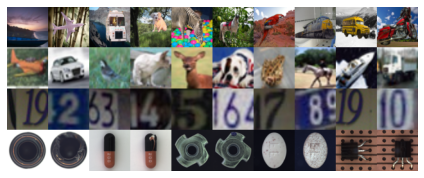
\includegraphics[width=\textwidth]{data/chapter_sgvaegan/fig5_all_grid.png}
    \caption{Examples of the datasets used in the experiments. Datasets from the top row to bottom: COCOPlaces, CIFAR10, SVHN2, and MVTec-AD. MVTec-AD examples of normal and anomalous samples from the \textit{bottle, capsule, metal nut, pill}, and \textit{transistor} classes are shown.}
    \label{fig:all_grid}
\end{figure}

\begin{description}
    \item[\textbf{Wildlife MNIST}]~\cite{sauer2021counterfactual} is an artificial dataset based on standard MNIST~\cite{lecun2010mnist}. For each MNIST digit, a background and foreground texture is sampled from a texture dataset described in~\cite{cimpoi2014describing} to create a colored version. Two versions of this dataset were created - \textit{mixed} and \textit{non-mixed}. In the mixed version, the background and foreground for each digit are sampled randomly from 10 background and foreground texture classes to create a very diverse set of images. In the non-mixed version, the background and foreground class is kept the same for all basic MNIST digits from the same class, resulting in a less diverse dataset. For examples of the non-mixed version, see the top row of Fig.~\ref{fig:wmnist_grid}. Each version contains 60000 samples of 32x32 pixel RGB images with three factors of variation.
    
    \item[\textbf{COCOPlaces}] is a dataset created similarly to Wildlife MNIST. 10 classes of objects from the COCO dataset~\cite{lin2014microsoft} were combined with 10 background classes from the Places dataset~\cite{zhou2017places}. Again, mixed and non-mixed variants were created. Because the object shape and texture cannot be separated in this case, it represents a problem with two factors of variation that is slightly more realistic than the previous one. Furthermore, it is much harder, as the object shapes are very distinct, sometimes the foreground object is only partially visible and the background itself may sometimes contain some other objects as well. A total of 5000 64x64 pixel RGB images were generated for each variant. For sample images of all classes, see~Fig.~\ref{fig:all_grid}.
    % the object classes are 'boat', 'airplane', 'truck','dog','zebra','horse','bird','train','bus','motorcycle'
    % the background classes are 'beach', 'bamboo_forest','canyon','broadleaf forest','ball_pit','orchard','rock_arch','shower','ski_slope','wheat_field'

    \item[\textbf{SVHN2}] is a well-known benchmark dataset~\cite{netzer2011reading} containing images of house numbers. In this cropped version of the dataset, the target digit is centered in the middle of the picture. However, there may be partial digits adjacent to it, which makes the problem harder. Furthermore, there are no available annotations for the background/foreground factor and in this paper, it is included mainly as a benchmark for comparison to other baseline methods. There are 10 classes for a total of 99288 32x32 pixel RGB images. The distribution of classes is uneven and ranges from 6 to 19 thousand samples. 
    
    \item[\textbf{CIFAR10}] is another classical dataset of images of 10 classes of different objects or animals often used for validation of anomaly detectors~\cite{ruff2018deep, ruff2019deep, chalapathy2018anomaly}. For an overview of the dataset see~\cite{krizhevsky2009learning}. There is a total of 60000 32x32 pixel RGB images.

    \item[\textbf{MVTec-AD}] is an industrial dataset~\cite{bergmann2019mvtec} that captures several different problems of identifying faulty or damaged objects. We have considered only the problems where there is a distinct object in the foreground, such as \textit{bottle} or \textit{metal nut}. The individual problems are smaller --- on average about 200 normal and 100 anomalous samples. The images used in our experiments are downscaled to 128x128 pixels.
    
\end{description}


The CIFAR10~\cite{krizhevsky2009learning}, SVHN22~\cite{netzer2011reading} and MVTec-AD~\cite{bergmann2019mvtec} are publicly available datasets. 

\chapter{Additional resources} \label{sec:appendix_links}

Most of the datasents from Appendix~\ref{sec:appendix_datasets} are publicly available. The Wildlife MNIST and COCOPlaces datasets were created and published by the authors of this paper and are available at \url{https://zenodo.org/record/7602025} and \url{https://zenodo.org/record/7612053}. The data that were produced during the extensive experimental comparison are not publicly available, since they exceed 10TB in size, but the model performance metrics from experiments in Chapters~\ref{sec:chapter_comparison} and~\ref{sec:chapter_sgvaegan} are available upon request from the authors.

Most of the models which wre experimented with experiments were implemented either mostly in the Julia~\cite{Julia-2017} language, with the exception of the SGVAEGAN model, which was implemented in PyTorch~\cite{NEURIPS2019_9015}. Now we list the publicly available repositories used in the creation of this thesis.

\begin{enumerate}
    \item Repository \url{https://github.com/vitskvara/UCI.jl} provides easy access to anomaly benchmark datasets that were created from classification problems in the UCI dataset database. This was used for the experiments with tabular data in Chapter~\ref{sec:chapter_comparison}.
    \item Repository \url{https://github.com/vitskvara/AlfvenDetectors.jl} is a collection of model code and utilities for experiments on Alfvén detection that was described in Sec.~\ref{sec:alfven}.
    \item Repository \url{https://github.com/aicenter/GenerativeModels.jl} contains a very general interface for training and evaluation of basic generative models.
    \item Repository \url{github.com/vitskvara/GenerativeAD.jl} compiles the experimental framework used for the large scale experimental comparisons in Chapters~\ref{sec:chapter_comparison} and~\ref{sec:chapter_sgvaegan}.
    \item Finally, the repository \url{github.com/vitskvara/sgad} contains the PyTorch implementation of the SGVAEGAN model.
\end{enumerate}



% ------------------------------------------------------------------------------
% Bibliography
% ------------------------------------------------------------------------------
\cleardoublepage
\phantomsection

\addcontentsline{toc}{chapter}{Bibliography}
\bibliography{references.bib}
\bibliographystyle{unsrt}

\end{document}